% =============================================================
%  dissertation.tex
%  Top-level container for the full dissertation.
%  Title: "From Surface to Core, Opening New Windows into the
%          Chemistry of Planets through Novel Methods in
%          Mass Spectrometry and Machine Learning"
%  Author: Ben Thyer
%
%  Compile with: pdflatex > biber > pdflatex > pdflatex
%  (or latexmk -pdf -biber dissertation.tex)
% =============================================================

\documentclass{caltech_thesis}

% Shared preamble (packages, commands, settings)
% =============================================================
%  dissertation_preamble.tex
%  Shared package imports and custom commands.
%  \input this file at the top of dissertation.tex ONLY.
% =============================================================

% --- Page geometry -----------------------------------------------------------
% NOTE: caltech_thesis.cls already loads `geometry` itself (1.5in side
% margins, 1in top/bottom, per Caltech's binding/margin requirements), so
% this preamble must NOT load it again with different options -- LaTeX
% would apply whichever load wins and silently ignore the other, which is
% exactly the kind of margin mismatch that gets a thesis bounced at
% submission. If dissertation.tex is ever compiled under a different
% (non-Caltech) document class that does NOT already set geometry, restore
% a line like `\usepackage[margin=1in, letterpaper]{geometry}` here.

% --- Typography --------------------------------------------------------------
\usepackage{lmodern}          % scalable Latin Modern fonts
\usepackage[T1]{fontenc}
\usepackage[utf8]{inputenc}
\usepackage{microtype}        % improved justification
\usepackage{textcomp}         % \textperthousand (per mille, U+2030) below --
                               % most other common unicode punctuation (curly
                               % quotes, en/em dash, degree, plus-minus,
                               % ellipsis) is already handled by inputenc's
                               % utf8 definitions and needs nothing extra.

% A few characters straight from pasted/pandoc-converted source text (e.g.
% Chapter 5's field-report content, which uses literal Greek delta for
% isotope notation like the literal characters "delta-18-O" rather than $\delta^{18}$O) aren't
% in inputenc's default utf8 active-character table and would otherwise be a
% fatal "Unicode character ... not set up for use with LaTeX" error. Map them
% here once, globally, rather than hand-converting every instance in the
% source text (safer -- avoids silently mistyping a value while
% converting).
\usepackage{newunicodechar}
\newunicodechar{δ}{\ensuremath{\delta}}
\newunicodechar{Δ}{\ensuremath{\Delta}}
\newunicodechar{‰}{\textperthousand}

% --- Math --------------------------------------------------------------------
\usepackage{amsmath, amssymb, amsthm}
\usepackage{bm}               % \bm bold math -- used by Chapter 4 (nGibbs methods)
\usepackage{siunitx}          % consistent SI units, e.g. \SI{4.2}{\mega\year}

% --- Figures & tables --------------------------------------------------------
\usepackage{graphicx}
\usepackage{calc}             % arithmetic in lengths (\real{}, +, -, *) -- needed
                               % by Pandoc-generated longtable column specs like
                               % p{(\linewidth - 12\tabcolsep) * \real{0.1951}},
                               % used by Chapter 3's Table 1 (Chapter3/Writing/
                               % HeInSulfides_Main_Body.tex)
\usepackage{float}
\usepackage{placeins}         % \FloatBarrier -- forces pending floats to
                               % resolve before a fixed point (e.g. right
                               % before a non-floating longtable/supertabular
                               % caption) without pinning them to their
                               % source position via [H], which can force a
                               % float onto a page it doesn't fit on and run
                               % it off the bottom margin. See chapter1_SI_
                               % body.tex (fig:predicted-vs-measured-permeation)
                               % for the case this was added for.
\usepackage{booktabs}         % professional table rules
\usepackage{longtable}        % tables that span pages
\usepackage{supertabular}     % multi-page table in Chapter 1 (apatite step-heat
                               % data), shared verbatim with TubeMethodPaper.tex,
                               % which loads supertabular natively via copernicus.cls
\usepackage{multirow}
\usepackage{caption}
\usepackage{subcaption}
\usepackage{array}           % extended column-spec features (>{...},
                              % \newcolumntype); harmless to keep loaded
                              % even though no table currently needs it
                              % now that Chapter 1's widest tables moved
                              % to \chplandscape (landscape) instead of
                              % font-shrinking -- see chapter1_body.tex.
\usepackage{pdflscape}        % \landscape environment, used via the
                              % \chplandscape wrapper (defined per-wrapper
                              % in Chapter1/chapter1.tex and Chapter1/
                              % chapter1_SI.tex) to rotate Chapter 1's
                              % widest tables for extra width in the
                              % thesis only -- the standalone
                              % TubeMethodPaper.tex/Paper/SI.tex define
                              % \chplandscape as a no-op instead, keeping
                              % those journal manuscripts portrait.

% Auto-center every table and shrink its text, without editing individual
% tables. Caltech's required 1.5in side margins leave only a 5.5in text
% width -- narrower than most of these tables were originally drafted for,
% which is why they were rolling off the right edge while left-justified.
%
% NOTE: an earlier version of this tried to wrap every \tabular in an
% adjustbox (\AtBeginEnvironment{tabular}{\begin{adjustbox}{max
% width=\textwidth}}) to hard-guarantee a fit regardless of native column
% widths. That broke the build (fatal "Missing }"/"invalid character"
% errors) -- \AtBeginEnvironment cannot safely wrap an environment that
% takes a mandatory brace argument (tabular's {column-spec}) in another
% such environment, because the injected \begin{adjustbox}{...} steals the
% argument-parsing slot tabular expects for its own column spec. Plain
% declarations (\centering, \footnotesize, \scriptsize -- no arguments of
% their own) are safe here; wrapping one environment inside another via
% this mechanism is not.
\AtBeginEnvironment{table}{\centering\footnotesize}
\AtBeginEnvironment{longtable}{\centering\scriptsize}
\AtBeginEnvironment{supertabular}{\centering\scriptsize}
\setlength{\tabcolsep}{3pt}   % default is 6pt -- tighter padding buys back
                              % real width on many-column numeric tables

% A few of the widest tables use fixed-width p{...} columns (in cm) rather
% than content-driven columns, so shrinking the font alone doesn't reclaim
% any width -- those still need a per-table \resizebox wrap (done directly
% in the affected .tex files, not here) for a hard guarantee of fit.
\graphicspath{
  {figures/}
  {Chapter1/Figures/source/}
  {Chapter1/Figures/generated/}
  {Chapter2/Figures/source/}
  {Chapter2/Figures/generated/}
  {Chapter3/Figures/source/}
  {Chapter3/Figures/generated/}
  {Chapter3/Figures/generated/step_heat_regressions/}
  {Chapter4/Figures/}
  {Chapter4/Figures/generated/}
  {Chapter5/Figures/}
  {Chapter5/Figures/source/}
  {Chapter5/Figures/generated/}
  {ChapterA/Figures/}
}

% --- Colors & hyperlinks -----------------------------------------------------
\usepackage[dvipsnames]{xcolor}
\usepackage{colortbl}         % \cellcolor shading in the Chapter 4 quality tables
\usepackage[
  colorlinks = true,
  linkcolor  = NavyBlue,
  citecolor  = OliveGreen,
  urlcolor   = Maroon,
  pdftitle   = {From Surface to Core},
  pdfauthor  = {Ben Thyer},
]{hyperref}
\usepackage{doi}

% --- Bibliography ------------------------------------------------------------
% Name-truncation rule (discipline convention, not a Caltech requirement --
% Caltech's thesis guidelines explicitly leave reference/citation style to
% "the style current in the thesis writer's discipline," only requiring it be
% used consistently throughout): 2-author works print both names; 3+-author
% works truncate to the first author + "et al." (maxnames=2, minnames=1).
% uniquelist=true is the standard biblatex safety net for the case where two
% DIFFERENT works would otherwise truncate to an identical-looking citation
% (e.g. "Smith et al., 2020" for two unrelated Smith-led 2020 papers) -- it
% expands the printed name list just enough to tell them apart (e.g. "Smith,
% Jones, et al." vs. "Smith, Brown, et al.") rather than appending a/b/c
% letters. True letter disambiguation (2020a / 2020b) already happens
% automatically -- with no extra config -- whenever two entries share the
% exact same full author list AND year (e.g. a genuine same-author same-year
% duplicate); it does not, by default, cover the "different authors, same
% truncated display" case, which is what uniquelist handles instead. As of
% this writing, a scan of references.bib found zero actual collisions under
% the new maxnames=2 rule, so this is a forward-looking safety net, not a
% fix for a live problem.
%
% maxbibnames is set high (effectively "no truncation") so the References
% list at the end always spells out every author, regardless of how the
% in-text citation truncates -- maxnames/minnames above only govern in-text
% \citep/\citet, not the bibliography.
\usepackage[
  backend    = biber,
  style      = authoryear,   % change to e.g. agu or geology if preferred
  sorting    = nyt,
  maxnames   = 2,
  minnames   = 1,
  maxbibnames = 99,
  uniquelist = true,
  giveninits = true,
  uniquename = init,
  natbib     = true,         % provides \citep/\citet/\citealp (natbib syntax),
                              % which Chapter 1's shared body (reused from
                              % TubeMethodPaper.tex) uses throughout. Without
                              % this, biblatex only offers its own
                              % \parencite/\textcite commands.
]{biblatex}
\addbibresource{references.bib}   % master .bib file — keep alongside dissertation.tex

% --- Header / footer ---------------------------------------------------------
\usepackage{fancyhdr}
\pagestyle{fancy}
\fancyhf{}
\fancyhead[LE,RO]{\thepage}
\fancyhead[RE]{\textit{\leftmark}}
\fancyhead[LO]{\textit{\rightmark}}
\renewcommand{\headrulewidth}{0.4pt}

% caltech_thesis.cls sets headsep to a very tight ~0.25in - 1em (roughly
% 6pt), tuned for its own default page style, which puts only a bare page
% number in the header. Since fancyhdr above instead puts the italicized
% chapter/section title (\leftmark/\rightmark) in the header, long titles
% that wrap to a second line collide with the body text below. Calling
% \geometry{} again (rather than re-\usepackage-ing it) only updates the
% keys given here and safely recomputes \textheight to match -- it does
% NOT reload/conflict with the page-margin setup the NOTE above warns
% about. headheight=30pt comfortably fits two lines of a 12pt header;
% headsep=18pt keeps a clean gap below it. If a chapter title ever needs
% a third header line, bump headheight further (e.g. to 42pt).
\geometry{headheight=30pt, headsep=18pt}

% --- Chapter / section formatting --------------------------------------------
% NOTE: caltech_thesis.cls (memoir-based) already defines its own official
% Caltech chapter styling -- centered, italic small-caps "Chapter I" numbering
% in Roman numerals via \chapnamefont/\chaptitlefont/\printchapterheading -- so
% titlesec's \titleformat{\chapter} override below has been disabled. Loading
% titlesec's chapter redefinition on top of memoir's own chapter-heading system
% is a known source of conflicts/incompatibility warnings. Re-enable this only
% if compiling Chapter files under a plain `book`/`report` class instead.
% \usepackage{titlesec}
% \titleformat{\chapter}[display]
%   {\normalfont\Large\bfseries}{\chaptertitlename\ \thechapter}{20pt}{\Huge}
% \titlespacing*{\chapter}{0pt}{40pt}{20pt}

% --- Per-chapter Supplementary Information (SI) -------------------------------
% Each chapter's SI (Chapter<N>/chapter<N>_SI.tex) is \input{} immediately
% after that chapter's main body, inside the SAME \chapter{} -- it is not a
% chapter of its own. Two problems that creates, and how these commands fix
% them:
%
% 1. Visually, the SI used to just continue as the next plain \section{},
%    indistinguishable from the chapter's own sections. \SItitlepage{...}
%    gives it a proper divider/title page first (unnumbered, no header, own
%    page), the way a book's appendix or backmatter would get one.
%
% 2. Numerically, its \section headings used to continue the chapter's own
%    numbering (...7, 8, 9...), so a reader landing mid-SI from a link or a
%    flipped-to page couldn't tell from the running header alone whether they
%    were still in the chapter proper or in its supplement. The `ChapterSI`
%    environment resets the section counter and switches \thesection to a
%    "<chapter>.<n>s" format for everything between \begin{ChapterSI} and
%    \end{ChapterSI} (e.g. the SI's first section becomes "1.1s" instead of
%    continuing on from wherever the main text left off). \thesubsection
%    inherits this automatically, since its default definition already
%    builds on \thesection. \S\ref{}/running headers/the ToC all pick this
%    up for free, because \setcounter and \renewcommand are both local by
%    default, and LaTeX environments are always wrapped in their own group,
%    so everything reverts automatically at \end{ChapterSI} with no matching
%    "restore" step to maintain. (The *next* chapter's own section numbering
%    isn't at risk even without that revert -- \chapter{} always resets
%    \c@section to 0 globally on its own, regardless of whatever it was left
%    at.)
%
%    NOTE on naming, two dead ends hit along the way, for the record:
%     (a) This is a `\newenvironment`, not a pair of \newcommand{\beginSI}/
%         \newcommand{\endSI} macros -- LaTeX reserves all command names of
%         the form \end<word> for environment closers, so
%         \newcommand{\endSI}{...} is flatly illegal ("Or name \end...
%         illegal", LaTeX2e kernel restriction, independent of memoir/
%         caltech_thesis.cls). Defining it as a proper environment sidesteps
%         that and is the more idiomatic way to express "everything between
%         these two markers" in LaTeX anyway.
%     (b) The environment is named `ChapterSI`, not `SI` -- \newenvironment{SI}
%         would auto-generate \SI as its begin-code control sequence, which
%         collides with siunitx's own \SI{value}{unit} command (loaded
%         above, e.g. \SI{4.2}{\mega\year}). `ChapterSI` generates
%         \ChapterSI/\endChapterSI instead, which don't collide with
%         anything.
%    Repeat this same \SItitlepage{...}/\begin{ChapterSI}...\end{ChapterSI}
%    pattern for Chapter 2 and beyond's SI wrappers.
\newcommand{\SItitlepage}[1]{%
  \clearpage
  \thispagestyle{empty}
  \vspace*{\fill}
  \begin{center}
    {\Huge\bfseries Supplementary Information}\\[1.5em]
    {\Large for Chapter \thechapter: \itshape #1}
  \end{center}
  \vspace*{\fill}
  \clearpage
}
\newenvironment{ChapterSI}{%
  \setcounter{section}{0}
  \renewcommand{\thesection}{\thechapter.\arabic{section}s}
}{}

% --- Appendix ----------------------------------------------------------------
% NOT loaded explicitly: memoir (which caltech_thesis.cls is built on) already
% emulates the `appendix` package internally with its own default options, so
% an explicit `\usepackage[toc, page]{appendix}` here causes a fatal "Option
% clash for package appendix" error. The `\begin{appendices}...\end{appendices}`
% environment used in dissertation.tex still works via memoir's built-in
% emulation without loading the package separately.

% --- Miscellaneous -----------------------------------------------------------
\usepackage{enumitem}
% pdflscape already loaded above (Figures & tables section) for \chplandscape
\usepackage{pdfpages}         % include external PDFs (field maps, etc.)
\usepackage{soul}             % \hl{} highlighting -- used once in Chapter 2's
                               % shared body (chapter2_body.tex)
\usepackage{lineno}           % line numbers — comment out for final version
% \linenumbers

% --- Code listings with cached output ------------------------------------------
% A script is shown verbatim with \lstinputlisting[style=thesispython], followed
% by what it printed (\cachedoutput) and the figure(s) it drew. Results are
% never computed by LaTeX: Chapter4/Figures/run_cached_listing.py runs the script
% once and writes generated/<stem>/{prints.txt,fig1.pdf,...}, rerunning only when
% the script's source changes (`make listings`). Paths are relative to the
% dissertation root.
\usepackage{listings}
\lstdefinestyle{thesispython}{
  language=Python,
  basicstyle=\ttfamily\footnotesize,
  keywordstyle=\color{NavyBlue}\bfseries,
  commentstyle=\color{OliveGreen}\itshape,
  stringstyle=\color{BrickRed},
  numbers=left, numberstyle=\tiny\color{gray}, numbersep=6pt,
  frame=single, rulecolor=\color{gray!60},
  breaklines=true, columns=fullflexible, keepspaces=true,
  showstringspaces=false, upquote=true,
}
\lstdefinestyle{thesisoutput}{
  basicstyle=\ttfamily\footnotesize,
  frame=leftline, framerule=1.5pt, rulecolor=\color{gray!60},
  backgroundcolor=\color{gray!8}, xleftmargin=1em,
  breaklines=true, columns=fullflexible, keepspaces=true,
}
% \cachedoutput{<path to prints.txt>} -- placeholder box instead of a fatal
% error if the cache hasn't been generated yet (e.g. fresh clone).
\newcommand{\cachedoutput}[1]{%
  \IfFileExists{#1}%
    {\lstinputlisting[style=thesisoutput]{#1}}%
    {\fbox{\footnotesize Missing cached output \texttt{\detokenize{#1}} -- run \texttt{make listings}}}}

% --- Custom commands ---------------------------------------------------------
\newcommand{\degC}{\ensuremath{^\circ\mathrm{C}}}
\newcommand{\He}{\textsuperscript{4}He}
\newcommand{\UThHe}{U--Th/He}
\newcommand{\fO}{\ensuremath{f_{\mathrm{O_2}}}}
\newcommand{\fS}{\ensuremath{f_{\mathrm{S_2}}}}
\newcommand{\fH}{\ensuremath{f_{\mathrm{H_2O}}}}
\newcommand{\Ea}{\ensuremath{E_a}}
\newcommand{\todo}[1]{\textcolor{red}{\textbf{[TODO: #1]}}}
\providecommand{\code}[1]{\texttt{\detokenize{#1}}}


% --- Title-page metadata (caltech_thesis.cls macros) --------------------------

\title{Recipes for Rare Metal Ores: Magmas, Metasomatism, and Meteoric Mobilization 
via Sulfide/Goethite (U-Th)/He Geochronology and ML-Accelerated Thermodynamic Modeling}
\author{Ben J. Thyer}
\copyyear{2026}
\defenddate{11/11/2026} 
\orcid{0000-0002-5341-0316}

% =============================================================
\begin{document}
% =============================================================

% ---- Front matter -----------------------------------------------------------
\frontmatter

% --- Title page + copyright page ----------------------------------------------
% \maketitle (defined by caltech_thesis.cls) typesets the Caltech title page

\maketitle

% --- Abstract ----------------------------------------------------------------
% The `abstract` environment is redefined by caltech_thesis.cls to render as
% an unnumbered, TOC-listed chapter (\extrachapter{Abstract}).
\begin{abstract}
\todo{Write abstract.}
\end{abstract}

% --- Acknowledgements --------------------------------------------------------
% caltech_thesis.cls provides both `acknowledgments` and `acknowledgements`
% (plural preferred) as unnumbered, TOC-listed chapters, same mechanism as
% `abstract` above.
\begin{acknowledgements}
\todo{Write acknowledgements.}

I am deeply grateful... 

The fieldwork at Draaikraal would not have been possible... 

Finally, I thank family/friends for their unwavering support...
\end{acknowledgements}

% --- Table of contents -------------------------------------------------------
\tableofcontents
% \listoffigures % Temproarily commented out to save space in the draft. Uncomment for final version.
% \listoftables

% ---- Main matter ------------------------------------------------------------
\mainmatter

% --- Introduction (unnumbered) -----------------------------------------------
\extrachapter{Introduction}
\markboth{Introduction}{Introduction}

\todo{Write short dissertation introduction, longer than abstract, detail each chapter.}

% --- Chapters ----------------------------------------------------------------
% =============================================================
%  Chapter 1 — A Simple Method for Helium Step Heat Experiments
%  at High Water or Sulfur Fugacity
%
%  This chapter is the dissertation-formatted version of
%  Chapter1/Writing/TubeMethodPaper.tex (the Copernicus/Geochronology
%  journal submission). Both wrappers \input{} the SAME shared
%  content files -- Chapter1/Writing/chapter1_abstract.tex and
%  Chapter1/Writing/chapter1_body.tex -- so the science is written
%  and edited in exactly one place. If you need to change the
%  text, equations, figures, or tables, edit those two files, not
%  this one or TubeMethodPaper.tex.
%
%  NOTE: Do NOT include \documentclass or \begin{document} here.
%        This file is \input{} into dissertation.tex.
% =============================================================

\chapter{A Simple Method for Helium Step Heat Experiments at High Water or Sulfur Fugacity}
\label{ch:apparatus}

% --- Chapter abstract / summary -----------------------------------------------
\begin{quote}
  \itshape
  % =============================================================
%  chapter1_abstract.tex
%  Shared abstract text for Chapter 1 / TubeMethodPaper.tex.
%
%  Kept separate from the surrounding \begin{abstract}...\end{abstract}
%  wrapper because that environment is NOT class-agnostic: under
%  copernicus.cls it renders in place as the paper's abstract, but
%  under caltech_thesis.cls the `abstract` environment is redefined
%  to break out into a new unnumbered "Abstract" chapter (via
%  \extrachapter), which is only appropriate once, at the front of
%  the whole dissertation (see dissertation.tex's own Abstract
%  chapter) -- not again in the middle of Chapter 1. So each wrapper
%  supplies its own environment/heading around this same raw text.
%
%  Edit this file (not TubeMethodPaper.tex or chapter1.tex directly)
%  to keep the journal paper and the dissertation chapter in sync.
% =============================================================
Helium isotope studies and U-Th/He geochronology of sulfur-bearing and hydrous minerals offer direct windows into the timing and context of hydrothermal mineralization, provided the conditions governing radiogenic helium retention and loss in nature are known. However, assessing helium retentivity at elevated temperatures is currently hampered by these minerals\textquotesingle{} instability under the high-temperature, high-vacuum conditions of conventional helium step-heating experiments. This paper introduces a novel method for conducting helium step-heating experiments under hydrothermal and sulfur-saturated conditions, designed to extend our knowledge of helium diffusion kinetics in hydrous and sulfur-bearing mineral phases. In this approach, silica glass ampoules encapsulate the mineral of interest, maintaining internally sulfur- or water vapor-saturated conditions against the ultra-high vacuum of the surrounding extraction line, while the high helium permeability of fused silica permits quantification of evolved helium using standard temperature control and mass spectrometry procedures. This work presents the experimental framework and key equations necessary to deconvolve the processes of helium permeation through the silica ampoule from the thermally activated degassing of helium from the encapsulated mineral. Permeation lag is quantified with a first-order permeation model and removed by one of two routes: the \emph{permeation step method}, which measures the ampoule's residual helium directly with low-temperature permeation steps, or, where those yields fall to blank level, the \emph{bounding method}, which constrains that residual from above by assuming steady-state permeation during long steps. Both rest on the ampoule's permeation rate constant, which is measured during the experiment itself rather than taken from the literature. Validation experiments measuring helium permeation through empty ampoules and ampoules containing only water, sulfur, or Durango apatite demonstrate that permeation lag is readily correctable in well-designed experiments and characterize the extent to which water and sulfur influence the helium permeability of fused silica. While sulfur-saturated experiments are straightforward to carry out with this method, several tractable complications are identified for experiments when significant water is present. This method expands standard experimental capabilities to encompass mineral phases that decompose under high vacuum, including sulfides and iron oxyhydroxides, opening new avenues for thermochronometric investigation of hydrothermal systems.

\end{quote}

% --- Landscape environment for oversized tables --------------------------------
% chapter1_body.tex (shared with the standalone Copernicus paper,
% TubeMethodPaper.tex) wraps its widest tables in \chplandscape instead of
% pdflscape's \landscape directly, so the SAME shared file can behave
% differently per wrapper: here (the thesis), it rotates the page and
% gives the table the full ~8in landscape text width, so the table can
% run at normal/legible font size instead of being shrunk to fit a
% portrait 5.5in column. TubeMethodPaper.tex/Paper/SI.tex instead define
% \chplandscape as a no-op, keeping the journal manuscript in its
% original compact portrait form. Guarded so defining it here doesn't
% clash if chapter1_SI.tex (which needs the same environment for its own
% oversized tables) happens to load first in some future reordering.
\makeatletter
\@ifundefined{chplandscape}{%
  \newenvironment{chplandscape}{\begin{landscape}}{\end{landscape}}
}{}
\makeatother

% --- Shared body (Introduction through Conclusions) ---------------------------
% Figures for this chapter live in Chapter1/Figures/{source,generated}/ (see
% the \graphicspath entry in dissertation_preamble.tex).
% =============================================================
%  chapter1_body.tex
%  Shared, class-agnostic body of Chapter 1 / TubeMethodPaper.tex
%  (Introduction through Conclusions -- everything between the
%  abstract and the end-matter/bibliography).
%
%  \input{} by BOTH:
%    - Chapter1/Writing/TubeMethodPaper.tex   (Copernicus journal paper)
%    - Chapter1/chapter1.tex                (dissertation chapter, caltech_thesis)
%  so the scientific content never has to be maintained in two places.
%  Edit this file, not the two wrappers, for any content change.
%
%  Portability notes:
%   - \introduction / \conclusions (Copernicus shorthands for
%     \section{Introduction} / \section{Conclusions}) have been
%     expanded to plain \section{} calls below so this file has no
%     dependency on copernicus.cls.
%   - Tables use \tophline/\middlehline/\bottomhline (Copernicus's
%     names for booktabs' \toprule/\midrule/\bottomrule). The
%     \providecommand block just below defines them as booktabs
%     aliases ONLY if not already provided by the wrapping class
%     (copernicus.cls defines its own, so this is a no-op there).
%     Whichever wrapper does NOT already provide them must load the
%     `booktabs` package itself (dissertation_preamble.tex already does).
%   - The multi-page apatite step-heat table uses `longtable`, not
%     `supertabular` (switched from supertabular -- see the comment at
%     that table below for why). copernicus.cls does NOT load
%     `longtable` natively, unlike `supertabular`, so TubeMethodPaper.tex
%     loads it explicitly; the thesis side gets it from
%     dissertation_preamble.tex. The SI's other multi-page tables still
%     use `supertabular` (portrait) or `longtable` (the three
%     \chplandscape-wrapped ones) -- see chapter1_SI_body.tex.
%   - Cross-references to the SI (e.g. "supplementary Fig.~\ref{...}",
%     "supplementary Eq.~\eqref{...}") use real \ref{}/\eqref{} against
%     labels defined in chapter1_SI_body.tex. These resolve correctly in
%     the dissertation, where chapter1.tex and chapter1_SI.tex are both
%     \input{} into the same dissertation.tex document (shared .aux).
%     They will render as "??" in the standalone TubeMethodPaper.tex/
%     SI.tex compile, since those are two separate documents and
%     \ref{}/\eqref{} cannot resolve across them -- to be addressed
%     separately (e.g. reverting to manual "supplementary Fig. N" text,
%     or a cross-document referencing package) when preparing that
%     standalone submission.
% =============================================================
\providecommand{\tophline}{\toprule}
\providecommand{\middlehline}{\midrule}
\providecommand{\bottomhline}{\bottomrule}

\section{Introduction}

Noble gas geochronology and thermochronometry (\textsuperscript{40}Ar/\textsuperscript{39}Ar and U-Th/He) on hydrous and sulfur-bearing mineral phases such as hornblende, clay minerals, biotite, goethite, and pyrite have already been leveraged as a powerful tool for understanding regional thermal histories as well as the timing of iron or rare metal mineralization \citep{mcinnes2005,heim2006,vasconcelos2013,nomade2004,yakubovich2020,yakubovich2021}. The interpretation of these data, however, is often complicated by the fact that helium (or argon) within hydrous or sulfur-bearing phases often degasses differently in the laboratory and in nature \citep{hanson1975,lee1993,lo2000,farley2024}.

Experiments aiming to characterize the migration mechanisms and rates of noble gasses through hydrous phases yield different results when conducted under hydrothermal conditions as opposed to traditional experimental methods in vacuo. Hydrothermal step heat experiments for argon in biotite and hornblende showed higher retentivity and comparatively favored diffusive loss mechanisms relative to experiments conducted in vacuo, and these results are more likely to accurately reflect loss mechanisms in nature \citep{harrison1982,harrison1985}; however, such experiments are labor-intensive and comparatively inflexible relative to modern helium step heat methods \citep{farley1999}.

Recently, some workers have taken advantage of the high helium permeability and selectivity of pure silica glass when designing novel experimental methods for U-Th/He geochronology \citep{yakubovich2020,yakubovich2021}, but these ideas have only been applied in a limited way to characterize helium migration in sulfur-bearing or hydrous phases (e.g., monotonic ramped heating experiments: \citealp{yakubovich2019}). This work aims to apply decades of research on helium permeability, solubility, and diffusion in fused silica glass \citep[e.g.,][]{jones1953,norton1953,rogers1954,altemose1961,swets1961,doremus1966,masaryk1968,shelby1971,shelby1972,shelby1976,shackelford1972} to adapt existing agile step-heat methods \citep{farley1999} to investigate helium loss rates and mechanisms in sulfur-bearing and hydrous mineral phases. 

Encapsulating minerals in silica glass ampoules allows experimentalists to maintain hydrothermal or sulfur-saturated conditions within the ampoule without otherwise altering the experimental design. Depending on the thermodynamics of the phase of interest, this method may stabilize the phase at elevated experimental temperatures, allowing for detailed characterization of helium migration in sulfide and hydrous minerals that hitherto has remained poorly understood (Fig.~\ref{fig:mineral-grid}).

\begin{figure}[htbp]
\centering
% \renewcommand{\arraystretch}{1.3}
% \rotatebox{90}{...} (no options) rotates around the box's bottom-left
% corner, not its center -- next to a row of images much taller than the
% label text, that left "Pyrite" visibly anchored toward the bottom of its
% row while "Arsenopyrite" (long enough to nearly fill the row on its own)
% looked centered mostly by coincidence. \rotatebox[origin=c]{90}{...}
% rotates around the text's own center instead, which centers both labels
% against their image row regardless of word length.
\setlength{\tabcolsep}{4pt}
\begin{tabular}{cccc}
 & \textbf{Control} & \textbf{Buffered} & \textbf{Unbuffered} \\[2pt]

\rotatebox{90}{\textbf{Pyrite}} &
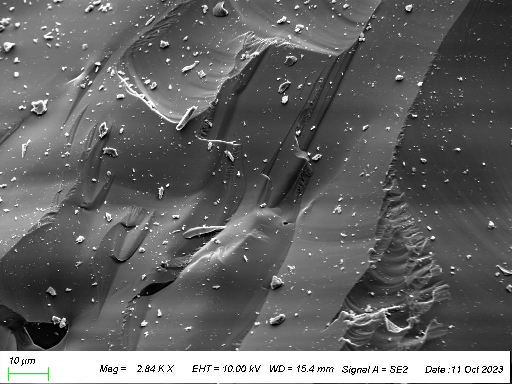
\includegraphics[width=0.28\textwidth]{LVPY_control_10um0.pdf} &
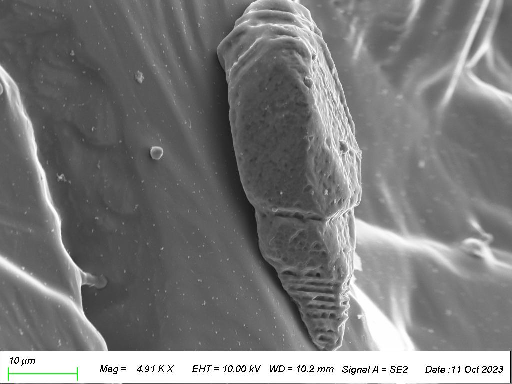
\includegraphics[width=0.28\textwidth]{LVPy_buff_600_8Hr_10um07.pdf} &
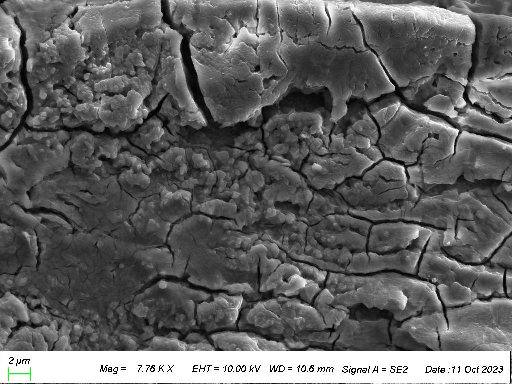
\includegraphics[width=0.28\textwidth]{LVPy_open_400_5Hr_2um11.pdf} \\[4pt]

\rotatebox{90}{\textbf{Arsenopyrite}} &
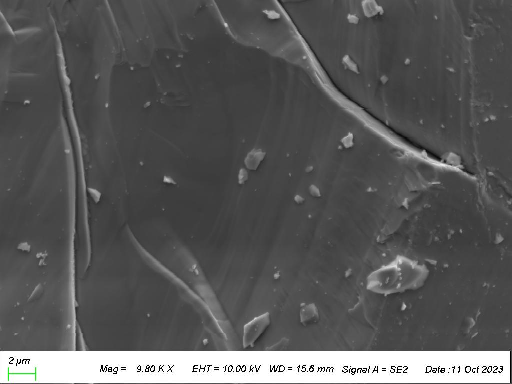
\includegraphics[width=0.28\textwidth]{Asp_control_2um7.pdf} &
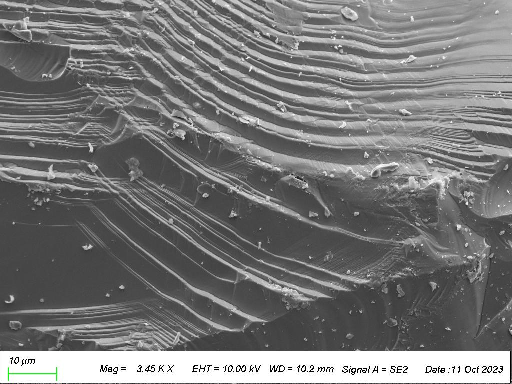
\includegraphics[width=0.28\textwidth]{asp_buff_400_8Hr_10um12.pdf} &
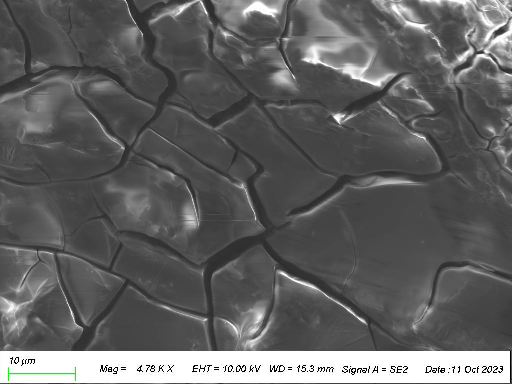
\includegraphics[width=0.28\textwidth]{Asp_bigClosed_400C_4hr_10um5.pdf} \\

\end{tabular}
\caption{Secondary electron SEM images of pyrite (top row) and arsenopyrite (bottom row) surface textures before heat treatment (control), and after heat treatment at 400°C for at least 4 hours, both unbuffered and buffered in a silica glass ampoule with fused sulfur or mineral realgar (AsS) for pyrite and arsenopyrite respectively. The buffered samples maintain the smooth surfaces and clear cleavage faces that the controls have, showing no evidence of decomposition. The unbuffered samples show clear evidence of decomposition by devolatilization, indicated by the formation of contraction cracks and surface roughening. Using silica glass ampoules to buffer samples within controlled microenvironments can prevent phase decomposition at the elevated experimental temperatures typical of helium step heat experiments. See the supplement \S\ref{sem-imaging-of-buffered-and-decomposed-sulfides} for details on the experimental methods and sample preparation.}
\label{fig:mineral-grid}
\end{figure}

\section{Experimental Methods}\label{experimental-methods}

\begin{figure}[t]
\centering
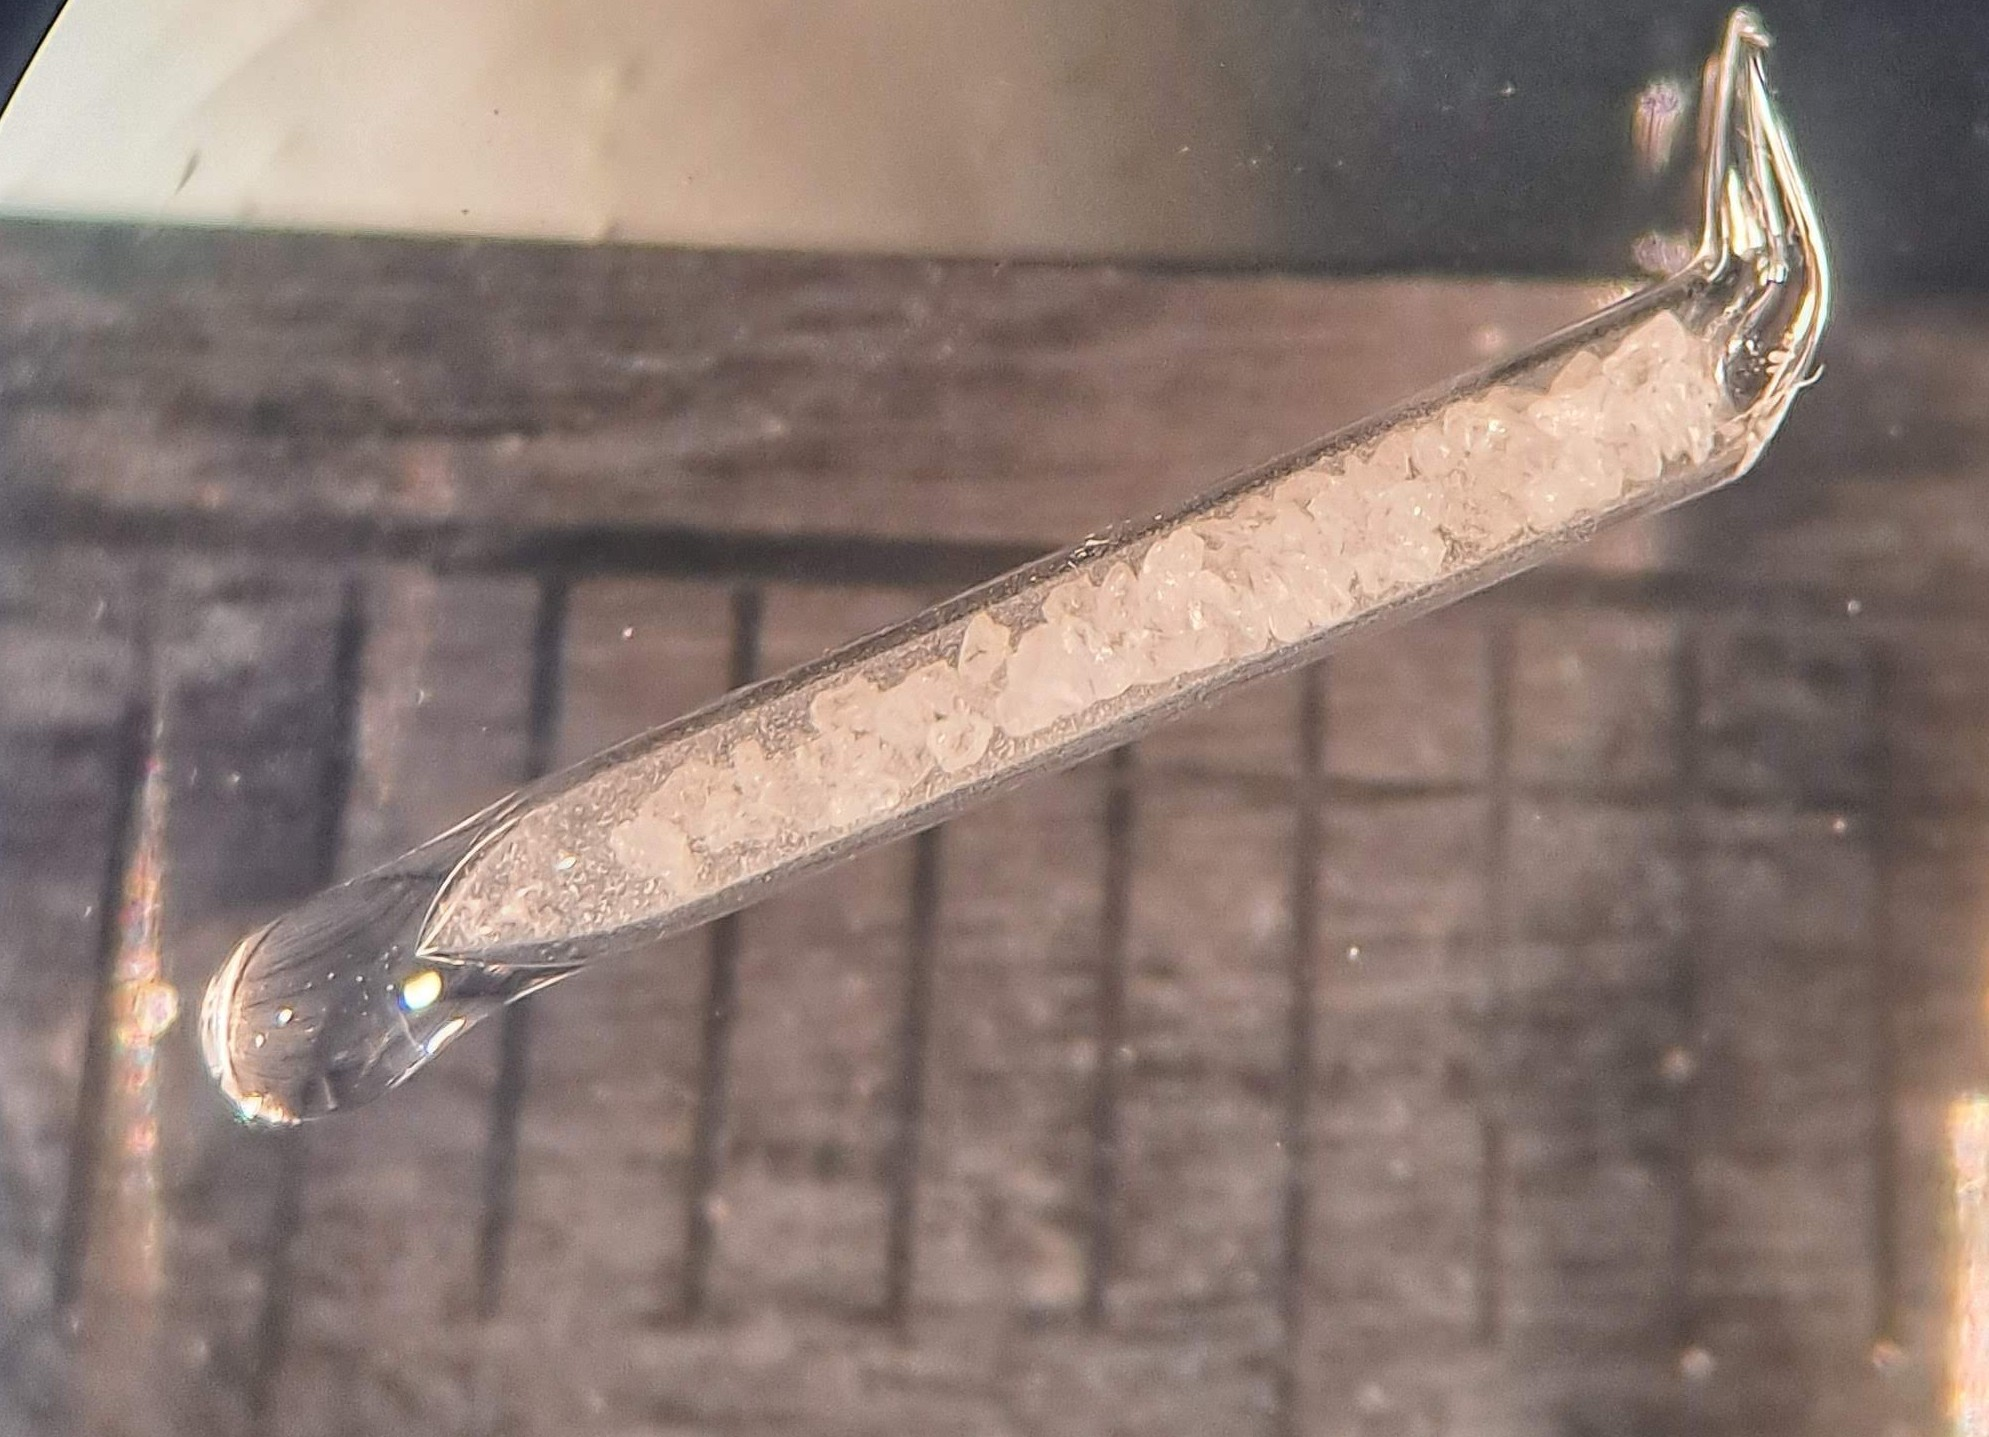
\includegraphics[width=8.3cm]{Apatite_tube.jpg}
\caption{A typical silica glass ampoule used for helium step heat experiments. The ampoule shown here contains Durango Apatite crushate sieved to 300 µm (radii $\approx$ 150 µm). The ampoule is roughly one cm long and one mm wide. The bars visible in the background are each separated by 1 mm.}
\label{fig:ampoule-photo}
\end{figure}

Five helium step heat experiments of sealed silica glass ampoules were undertaken at Caltech to demonstrate the applicability of equations derived here to real helium step heat experiments of geologic materials using a projector-lamp heating apparatus, described in detail in \citet{farley1999}. Four of these experiments involved introducing helium into empty, water-filled, and sulfur-filled ampoules, then measuring helium permeation to assess the applicability of theory outlined in this chapter to helium step heat experiments at Caltech, and to reproduce measurements of permeability rates from the literature \citep{norton1953,jones1953,swets1961,altemose1961}. The fifth experiment was a standard helium step heat experiment on encapsulated Durango apatite, a widely used standard for helium diffusion experiments and U-Th/He thermochronometry \citep{zeitler1987,wolf1996,farley2000,shuster2005,shuster2006,flowers2007}. The aim of that experiment was to be a practical test in deconvolving the process of helium permeation through silica glass ampoules from thermal helium loss of a well-studied geologic material. Table~\ref{tab:ampoule-dimensions} summarizes the dimensions, geometric factors, and encapsulated materials of this work.

% Fixed-width p{...} columns (13.6cm) don't shrink with font size alone --
% wrapped in \resizebox to hard-guarantee it fits the 5.5in Caltech text
% width. Safe here because this is a single-page `table`/`tabular` (not
% longtable/supertabular, which cannot be resizebox-wrapped). Kept in
% portrait (no \chplandscape) at the default \AtBeginEnvironment{table}{
% ...\footnotesize} size -- same treatment as the other tables -- per
% feedback that this table read oddly enlarged/landscaped relative to the
% rest and fit fine in portrait before.
\begin{table}[t]
\centering
\caption{Silica Glass tubes that were the subject of helium step heat experiments in this work. Ampoules labeled ``Quad'' had evolved 4He quantified by isotope dilution using a Pfeiffer Prisma QMS 200 quadrupole mass spectrometer, whereas ampoule labeled ``MC'' had both evolved 3He and 4He quantified using a Helix-MC-Plus\textsuperscript{10K} multi-collector mass spectrometer. Where 3He was measured, the ampoule was soaked in tank helium with an isotope ratio of \textasciitilde0.15 Ra}
\label{tab:ampoule-dimensions}
\resizebox{\textwidth}{!}{%
\begin{tabular}{p{1.8cm}p{1.4cm}p{1.8cm}p{1.8cm}p{1.8cm}p{1.2cm}p{1.8cm}p{2.2cm}}
\tophline
Ampoule Contents & Mass Spec. & Inner \newline Diameter \newline µm & Outer \newline Diameter \newline µm & Geometric factor \emph{G} \newline cm\textsuperscript{-2} & Volume Ratio $\left(\frac{V_{glass}}{V_{gas}}\right)$ & Content \newline Mass & Helium \newline Source \\
\middlehline
Empty & Quad & 630 & 960 & 4785.3  & 1.32 & --- & Atmosphere \\
Empty & MC & 747 & 1159 & 3263.9 & 1.41 & --- & Tank He \\
Sulfur & MC & 529--550 & 835--872 & 5992.1 & ~1.5 & \textasciitilde0.2 mg & Tank He \\
Water & MC & 487--515 & 734--776 & 7789 & 1.27 & \textasciitilde0.5 mg  & Tank He \\
Durango \newline Apatite & Quad & 850 & 1350 & 2393.5 & 1.52 & 3.18 mg & Radiogenic \\
\bottomhline
\end{tabular}%
}
\end{table}

To prepare the silica glass ampoules, \textasciitilde10 cm long segments of pure silica glass tubes with an outer diameter of 4 mm and an inner diameter of 3 mm were submerged and sonicated within acetone, ethanol, then MilliQ water baths in sequence, and then were dried overnight in a 100°C oven. The glass tubes were hand-pulled into thin pipettes with a jewelry welding torch and their thin ends were fused closed.

After the glass had cooled, degassed lab-grade sulfur, distilled water, or Durango apatite were added to some of the tubes. Two tubes were left empty. To seal, the top of each pipette was interfaced with a vacuum line and was pumped to a pressure of \textless0.1 torr. The encapsulated water tube was flash-frozen in liquid nitrogen and then pumped and sealed in a saltwater ice bath to selectively pump away atmospheric gasses and not water. Sublimation of sulfur and water ice during pumping was minor. The primary motivation for pumping the tube to rough vacuum was to aid the sealing process. After rough vacuum was achieved, a fine-tipped welding torch was used to seal the top of each ampoule. To determine the geometric factors for permeation of the ampoules, the inner and outer diameters of each ampoule were determined using the measurement function of the Amscope stereo microscope software, which was calibrated and tested during early development of this method.

Except for the encapsulated Durango apatite ampoule, helium gas needed to be introduced into the sealed ampoules before they were loaded into the projector lamp heating cells. About 15 nccSTP of atmospheric helium was introduced into the empty ampoule used for the quadrupole mass spectrometer experiment by heating the ampoule in a muffle furnace to \textgreater400°C in atmosphere overnight, which was sufficient to support a short permeation experiment of 4He. However, to conduct step heat permeation experiments on 3He, much larger quantities of helium were necessary. The encapsulated sulfur and water ampoules and the other empty ampoule were soaked in 2-20 torr of high purity tank helium with an isotope ratio of about \textasciitilde0.15 Ra at 300°C for about 24 hours. This procedure introduced 0.6-10 pccSTP 3He and up to 52,000 nccSTP 4He into each tube, allowing for measurements of both 3He and 4He permeation simultaneously.

The sealed ampoules were placed in copper foil packets and mounted to a K-type thermocouple within an ultra-high vacuum projector lamp heating cell described in more detail by \citet{farley1999}. Before each experiment began, each ampoule was washed with ethanol, air-dried, loaded in the lamp cell, pumped to high vacuum, and was held at 100°C for 30 minutes under dynamic vacuum to desorb ethanol, water, and other atmospheric species on the ampoule, copper packet, and lamp cell. Less than 0.5 ‰ of the radiogenic helium in 150µm radius Durango apatite would be expected to degas in 30 minutes at 100°C, which would amount to \textasciitilde0.01 nccSTP for this experiment, using the diffusion parameters of \citet{farley2000} and the forward equations of \citet{fechtigkalbitzer1966}. The atmospheric helium component within the encapsulated Durango Apatite ampoule constrained by permeation steps at the beginning of the experiment was much larger: 1.47 ± 0.18 nccSTP 4He.

We found that the fused silica ampoules were capable of maintaining surprisingly high internal pressures, but ampoules filled with water would often explode at temperatures above 315°C. It is recommended that experimentalists limit the temperature of water-filled ampoules to below 300°C. We have not observed any explosions of sulfur-filled ampoules at any temperature. 

Heating steps and isotopic measurements for all samples were automated using custom LabView routines with the exception of the tank helium-soaked empty tube experiment on the Helix-MC-Plus\textsuperscript{10K} multi-collector mass spectrometer after the 7\textsuperscript{th} measurement. For all other ampoules, a Watlow temperature controller held the ampoule at the temperature set point for a pre-programmed duration, after which the ampoule was allowed to cool while the evolved gas was prepared for measurement for about 25 minutes. After the first 7 measurements, the empty tube experiment on the Helix-MC-Plus\textsuperscript{10K} was instead set to an elevated temperature manually while the evolved gas was allowed to accumulate continuously in an attempt to mitigate uncertainties related to frequently changing temperatures (supplementary Eq.~\eqref{eq:s7-2}; Fig.~\ref{fig:thermal-perturbation-error}) and continued permeation at room temperature during gas cleanup and measurement. The accumulated gas was measured every 40-120 minutes. For this experiment, the temperature was changed either during the 1 minute pump-out of the lamp cell after inletting gas into the mass spectrometer, or a period of helium accumulation for measurement. When the temperature was changed during an accumulation period, no permeability was calculated for that step, and the measured abundances of those steps were used only to track the helium contents of the tube.

Helium isotope measurements of evolved gasses from steps heats of one empty silica glass ampoule and glass-encapsulated sulfur and water ampoules equilibrated with 2-20 torr of high purity tank helium (R $\approx$ 0.15 R\textsubscript{a}) were acquired at Caltech on a Thermo Fisher Helix-MC-Plus\textsuperscript{10K} mass spectrometer in peak hopping mode from November 19\textsuperscript{th}, 2023 to Feburary 15\textsuperscript{th}, 2024. Helium was purified by exposing evolved gasses to a charcoal trap held in liquid nitrogen, a titanium sponge getter, then a SAES NP10 getter before freely expanding into the Helix-MC-Plus\textsuperscript{10K}. 3He was measured with a pulse-counting electron multiplier, while 4He was detected on a Faraday detector. The majority of the analysis time was spent measuring 3He. Every few hours, the background was mass-scanned to set the 3He and 4He measure points; each was taken to be a constant mass offset from the background HD\textsuperscript{+} peak. These mass offsets are precisely measured when tuning the Helix-MC-Plus\textsuperscript{10K} for helium isotope analysis. Months of helium measurements with the Helix-MC-Plus\textsuperscript{10K} at Caltech have shown this approach to be reliable, reproducible, and accurate for helium isotope analysis. Additionally, an electron multiplier monitored atomic mass 3.5 to detect 4He overspray. 4He abundances were very large during these experiments, resulting in a small but measurable 4He overspray of up to 0.68 cps at mass 3.5. These overspray signals at mass 3.5 were always less than 1\% of the 3He signal at mass 3, suggesting that 4He overspray did not significantly affect 3He signals. Measurements of high 3He MM gas standard were analyzed every 8 hours (totaling 116 measurements) to track instrumental drift of 3He and 4He sensitivities and to quantify internal reproducibility. These standards show 3He was internally reproducible to within 5\% (2$\sigma$), whereas 4He was internally reproducible to within 2\% (2$\sigma$), where reproducibility is estimated as the standard deviation divided by the mean.

Helium-4 evolved during step heats of the empty silica glass ampoule equilibrated with atmosphere and the silica glass-encapsulated Durango apatite was quantified using isotope dilution with a high purity 3He spike on a Pfeiffer Prisma QMS 200 quadrupole mass spectrometer from October 30\textsuperscript{th} to November 10\textsuperscript{th}, 2023. Evolved gas from the ampoule in the lamp heating cell was allowed to mix with the 3He spike and the mixture was frozen on charcoal held at 14°K within a cryostat, then helium was selectively released to the mass spectrometer by raising the temperature to 36°K.

A standard gas with a known amount of 4He is routinely measured, at least one time per experiment, to monitor drift in the relative sensitivity of 3He and 4He on the Pfeiffer Prisma QMS 200 quadrupole mass spectrometer. Relative sensitivities are determined for each standard measurement and are linearly interpolated in time for sample measurements. Blanks are approximately 5 pccSTP \textsuperscript{4}He, which is very small compared to all interpreted \textsuperscript{4}He measurements.

\section{Theoretical Framework of Permeation Lag}\label{theoretical-framework-of-permeation-lag}

\begin{figure}[t]
\centering
\includegraphics[width=8.3cm]{Durango_Sim.pdf}
\caption{An illustrative simulation of the effects of permeation lag on step heat measurements of 150 µm radii spheres of Durango apatite encapsulated in a ``standard ampoule'' with an outer diameter of 1mm and inner diameter of 0.6mm, corresponding to a geometric factor \emph{G} of 4350.26 cm\textsuperscript{-2}. Some amount of helium degassed from the apatite during an experimental step remains in the tube during measurement and permeates out in later steps.  The heating schedule of this model system is given in Table~\ref{tab:heating-schedule}. This simple model assumes new temperatures and their corresponding steady-state diffusive concentration profile within the glass ampoule are reached instantaneously. Effects of diffusive disequilibrium, if considered, would change the permeated amount for each step by less than 5\%.}
\label{fig:durango-stepheat-lag-simulation}
\end{figure}

The process of helium permeation through thin walls of an ampoule is rapid but not instantaneous on experimental timescales. Helium evolved from encapsulated minerals is only available for measurement following permeation through the glass ampoule  (Fig.~\ref{fig:durango-stepheat-lag-simulation}), producing a predictable ``permeation lag'' effect in helium measurements that commonly manifests with undermeasurement of helium during prograde heating sequences and corresponding overmeasurement of helium produced during retrograde sequences (Fig.~\ref{fig:simulated-arrhenius-lag-artifact}). This is not merely a theoretical concern: Fig.~\ref{fig:durango-arrhenius-lag-corrected} shows the same artifact in real, uncorrected step heat data for the encapsulated Durango apatite experiment described above (\S\ref{experimental-methods}); the correction developed below is applied to this dataset in full in \S\ref{results} (Fig.~\ref{fig:durango-arrhenius-lag-corrected}).

\begin{figure}[t]
\centering
\includegraphics[width=8.3cm]{DurangoStepYields_RelativeAnomaly.pdf}
\caption{Measured-to-true yield ratio, \(m/\omega\), for the first 13 experimental steps (through the isothermal 300\textdegree C triplicate) of the real encapsulated Durango apatite step heat experiment described above (\S\ref{experimental-methods}) and tabulated in full in Table~\ref{tab:apatite-stepheat}, plotted in measurement order and labeled by nominal step temperature. Here \emph{m} is the raw measured helium yield for a step and $\omega$ is its permeation lag-corrected yield; bars are anchored at a ratio of 1 (no anomaly) on a logarithmic axis, so a doubling and a halving of the ratio are given equal visual weight. Steps taken while ramping to higher temperatures are generally undermeasured (blue), as some of the sample's evolved helium has not yet fully permeated out of the tube at the time of measurement, while steps taken while ramping to lower temperatures are generally overmeasured (red), as helium retained in the tube from earlier, hotter steps continues to permeate out. The first two steps (100-150\textdegree C) are strongly overmeasured despite being on the heating ramp because little helium had yet evolved from the apatite, so measured yield there is dominated by pre-existing atmospheric helium draining from the tube rather than fresh sample degassing.}
\label{fig:durango-stepwise-yields}
\end{figure}

\begin{figure}[t]
\centering
\includegraphics[width=8.3cm]{Apatite_diff_sim1.1.pdf}
\caption{An Arrhenius plot of apparent diffusivities inverted from modeled hypothetical measurements of an encapsulated sample of Durango apatite. Permeation lag produces a characteristic effect where measurements of prograde sequences of increasing temperature produce erroneously low apparent diffusivities when inverted using the equations of \citet{fechtigkalbitzer1966}, whereas retrograde (decreasing) temperature sequences exhibit the opposite effect. Diffusion parameters are taken from \citet{farley2000}.}
\label{fig:simulated-arrhenius-lag-artifact}
\end{figure}


\begin{table}[t]
\centering
\caption{Heating schedule for numerically modeled step heat experiment of silica glass encapsulated Durango apatite.}
\label{tab:heating-schedule}
\begin{tabular}{ll}
\tophline
Temperature (\textdegree C) & Time (min) \\
\middlehline
200 & 180 \\
250 & 120 \\
300 & 120 \\
350 & 120 \\
400 & 60 \\
325 & 120 \\
275 & 120 \\
250 & 120 \\
175 & 120 \\
\bottomhline
\end{tabular}
\end{table}

This effect can be modeled (and corrected for) for a system obeying the simple equation:

\begin{equation}
\label{eq:permlag}
n_{t} = n_{0} + \omega - m
\end{equation}

Where \(n_{t}\) is the amount of helium within the ampoule after time \emph{t}, \(n_{0}\) is the initial amount of helium within the ampoule (which is inherited from previous heating steps), \(\omega\) is the amount of helium evolved by the encapsulated sample during time \emph{t,} and \(m\) is the amount of measurable helium that has permeated out of the ampoule into the high-vacuum chamber during time \emph{t.}

Heating steps are consecutive, so the helium inventory quantified between two steps applies to both the previous and the subsequent step:

\begin{equation}
\label{eq:carry}
n_{t}^{\,i} = n_{0}^{\,i+1}, \qquad n_{0}^{\,i} = n_{t}^{\,i-1}
\end{equation}

Recovering \(\omega\) for a step therefore requires knowledge of the ampoule's helium content immediately before and immediately after it. Sections~\ref{permeation-step-method} and~\ref{bounding-method} give the two routes used in this work to obtain those quantities.

\begin{figure}[t]
\centering
\includegraphics[width=8.3cm]{encapsulated_DApErr.pdf}
\caption{An Arrhenius plot of a helium step heat experiment of silica-glass encapsulated Durango Apatite with 2$\sigma$ error bars. Without permeation lag corrections, the apparent diffusivities display highly irregular behavior that would be unrecognizable to this well-behaved sample -- exactly the artifact anticipated by the simulation of Fig.~\ref{fig:durango-stepheat-lag-simulation} above. With permeation lag corrections, the sample agrees well with the reported diffusive parameters of \citet{farley2000} for the appropriate sieve size ($r$ = 150\textmu m). As the experiment proceeds beyond temperatures of 300\textdegree C, the activation energy of diffusion decreases to reveal a slight downward curl, a phenomenon well-documented for Durango apatite likely due to annealing of crystal defects and radiation damage \citep{wolf1996,farley2000}. Apparent diffusivities are calculated with the equations of \citet{fechtigkalbitzer1966} with and without permeation lag corrections. Four measurements of the permeation lag corrected apparent diffusivities are within error of 0 at the 2$\sigma$ level and thus are excluded from the plot.}
\label{fig:durango-arrhenius-lag-corrected}
\end{figure}

Helium permeation through fused silica in diffusive steady state is a first order process that can be described with the simple differential equation:

\begin{equation}
\label{eq:permode}
\frac{dn}{dt} = \  - GKnRT
\end{equation}

Where \emph{n} is the number of helium atoms, \emph{t} is the time, \emph{G} is the geometric parameter in units of cm\textsuperscript{-2}, which is a function only of the geometry of the glass membrane, \emph{K} is the permeation constant for helium in fused silica, which follows the Arrhenius law: \(\left( K(T) = K_{0}e^{- \frac{E_{a}}{RT}} \right)\) and has been repeatedly measured for fused silica \citep{norton1953,altemose1961,swets1961,masaryk1968}, \emph{R} is the gas constant, and \emph{T} is the temperature in Kelvin. Equation~\eqref{eq:permode} is identical to the permeation equation used in early studies \citep{norton1953,altemose1961,swets1961,studt1962,masaryk1968}, except that it is formulated in terms of absolute atomic abundances instead of helium gas pressure by the ideal gas law. It is easily integrated by separation of variables to yield \(n_{t} = n_{0}e^{- GKRTt}\) (see supplement, \S\ref{a-ficks-law-formulation}, for details). Relating that result to the measured quantity through Eq.~\eqref{eq:permlag} in the absence of any release from the sample \(\left( m(\omega = 0) = n_{0} - n_{t} \right)\) gives an expression most intuitively stated in terms of the fraction of the ampoule's initial helium reservoir that permeates during time \emph{t}:

\begin{equation}
\label{eq:permsol}
^{He}F = \frac{m}{n_{0}} = 1 - e^{- \lambda t}, \qquad \lambda = KGRT
\end{equation}

Where \(^{He}F\) is the fractional permeation yield: the fraction of the ampoule's initial helium reservoir (\(n_{0}\)) that permeates as \(m\) (Eq.~\eqref{eq:permlag}) during a time \emph{t} of steady state permeation, and \(\lambda\) is the ampoule's permeation rate constant. Collecting \emph{K}, \emph{G}, \emph{R}, and \emph{T} into \(\lambda\) is useful because \(\lambda\) is the quantity that can be measured directly during an experiment (\S\ref{in-situ-rate-constant}), whereas \emph{K} and \emph{G} cannot be separated without independent knowledge of the ampoule geometry.

The geometric factor \emph{G} for a cylindrical membrane with negligible permeation through the top or bottom is determined using the effective area of permeation given by Masaryk, 1968:

\begin{equation}
\label{eq:geomfactor}
G = \frac{2}{a^{2}\ln\left( \frac{b}{a} \right)}
\end{equation}

where \emph{a} is the cylinder's internal radius, and \emph{b} is the external radius. There is no dependence on the cylinder length when permeation through the top and bottom are negligible. This geometric constant will vary according to the experimental design and therefore must be measured by the experimentalist.

Equation~\eqref{eq:permsol} is only strictly valid with two assumptions:

\begin{enumerate}
\def\labelenumi{\arabic{enumi}.}
\item
  The helium partial pressure in the ``measurable'' reservoir outside of the ampoule is negligible compared to the partial pressure within the ampoule. Because the ratio of typical ampoule and the diffusion cell volumes is \textasciitilde1/10,000 \citep{farley1999}, this assumption is essentially always reasonable.
\item
  The helium concentration profile within the ampoule's glass walls is in diffusive steady state between the inner and outer walls. The real steady state helium concentration profile is well-approximated by the ideal steady state profile for ampoules with a glass/gas volume ratio less than 2 (Figs.~\ref{fig:steady-state-profile-deviation},~\ref{fig:numerical-error-volume-ratio-control}). For these ampoules, \eqref{eq:permsol} is accurate to within 1\% after the establishment of a diffusive steady state. Additionally, the diffusive steady state assumption is ephemerally violated when the temperature is changed due to the temperature dependence of the glass/gas partitioning of helium. The ampoule should therefore be held at the permeation temperature for at least one diffusive timescale \(\tau = L^{2}/D\) after every temperature change before measuring, where \emph{L} is the wall thickness and \emph{D} the diffusivity of helium in silica glass \citep{swets1961}. In this work, low-temperature heating steps are repeated to allow for the new diffusive steady state concentration profile to become established. The ampoules of this work reach diffusive equilibrium in 30-70 minutes at 80° (Fig.~\ref{fig:diffusive-profile-reequilibration-time}, supplementary figures 10 and 11). Comparisons between the abundance of helium within glass as a function of temperature limits the error introduced by thermal perturbation to less than 5\% (supplementary figure 9).
\end{enumerate}

% \def\labelenumi{\alph{enumi}.}

\begin{figure}[t]
\centering
\includegraphics[width=8.3cm]{diffusive_EQM_fused_silica.pdf}
\caption{Timescales as a function of temperature to reestablish a steady state diffusive concentration profile for different glass thicknesses. These curves correspond to the timescales at which the Fourier number equals 1. 4He diffusivities are taken from \citet{swets1961}.}
\label{fig:diffusive-profile-reequilibration-time}
\end{figure}

\section{Experimental Approaches Addressing Permeation Lag}\label{experimental-approaches-addressing-permeation-lag}

A combination of analytical and experimental methods may be used to correct for permeation lag and properly account for all helium evolved from the sample. Some common practices for noble gas measurements may introduce error when using this method. For example, it is common practice to purify and collect emitted helium with the diffusion cell open to the vacuum line at room temperature for extended times, often 15-30 minutes, and it is assumed that no additional helium evolution occurs. This assumption is reasonable for commonly measured geological materials, but it can be problematic when unexamined during permeation steps of silica glass encapsulated materials because helium permeation in silica glass is significant even at room temperature. In this work, permeation during these waiting times is often mathematically corrected for using Eq.~\eqref{eq:permsol}, assuming permeation continues at room temperature. Alternatively, there are experimental approaches to address ongoing permeation during these waiting periods: they may be shortened to minimize their impact on the measurement, or the ampoule may be held at the warm permeation temperature during the gas purification and cryofocusing processes, so that permeation continues at the same temperature during this time without introducing complicated thermal histories.

From Eq.~\eqref{eq:permlag}, it is immediately clear that when the evolved helium \(\omega\) is large with respect to the amount of helium within the ampoule, \(n_{t}\) or \(n_{0}\), then \(\omega \approx m\) and permeation lag can be neglected. Unfortunately, this is not the case for most phases commonly subjected to helium step heat experiments with routine heating schedules (e.g. hour-timescale steps at 100-400°C for apatite or zircon), but it is sometimes possible to design an experiment with long time-steps where the total evolved helium is large compared to the amount of helium in-residence within the tube. Nonetheless, permeation lag can be quantified and corrected for in \emph{any} experiment where the encapsulated material is effectively closed to helium loss at room temperature. Two approaches are described here to recover the helium evolved from an encapsulated sample (\(\omega\)) from measured amounts (\emph{m}): the \emph{permeation step method} (\S\ref{permeation-step-method}), which measures the ampoule's helium inventory directly between experimental steps, and the \emph{bounding method} (\S\ref{bounding-method}), which constrains that inventory from above when it cannot be measured. Both require the ampoule's permeation rate constant, which should be measured during the experiment itself rather than assumed from the literature (\S\ref{in-situ-rate-constant}).

\subsection{The Permeation Step Method}\label{permeation-step-method}

In typical experimental heating steps, there are two fluxes of helium controlling the ampoule's helium abundance: an influx of helium evolved from the sample and an outflux of helium due to permeation. For lower temperature steps, for which helium release from the sample is negligible (\(\omega = 0\)), the helium abundance within the ampoule is controlled only by the process of helium permeation, simplifying Eq.~\eqref{eq:permlag} and allowing for Eqs.~\eqref{eq:permlag} and \eqref{eq:permsol} to form a system of equations that can be solved for \(n_{t}\) and \(n_{0}\ \)given a measurement \emph{m} for an isothermal heating step of known duration.

\begin{equation}
\label{eq:n0perm}
n_{0} = \frac{m}{^{He}F}
\end{equation}

Where \(^{He}F\) is the fractional permeation yield defined in Eq.~\eqref{eq:permsol}. Such a low temperature heating step is hereby referred to as a \emph{permeation step} in this work. A permeation step does double duty: through the step-to-step continuity of the ampoule's inventory, it constrains both the helium remaining after the preceding high temperature step and the helium inherited by the following one. Placing a permeation step after every high temperature \emph{experimental step} (\(\omega > 0\)) therefore supplies \(n_{t}\) and \(n_{0}\) throughout the experiment, and Eq.~\eqref{eq:permlag} returns the helium evolved from the natural sample, \(\omega\).

Equation~\eqref{eq:n0perm} requires the rate constant of permeation for the ampoule in use, \(\lambda = KGRT\). This may be assembled from the ampoule's measured dimensions through the geometric factor \emph{G} (Eq.~\eqref{eq:geomfactor}) together with a literature permeability coefficient \emph{K} for helium in fused silica, which has been measured repeatedly as a function of temperature \citep{norton1953,altemose1961,swets1961,masaryk1968}. Published values should not be relied upon, however, especially for hydrothermal experiments: water entering the glass changes its permeability \citep{shelby1972,tsuru2011}, and water-bearing ampoules show anomalously high rate constants (\S\ref{resolving-the-paradoxically-high-apparent-helium-permeability-in-water-filled-tubes}). The rate constant should instead be measured on the ampoule actually in use, during the experiment itself (\S\ref{in-situ-rate-constant}). That measurement is best understood as a prerequisite and extension of the permeation step method rather than as an alternative to it: the consecutive isothermal permeation steps it requires are already part of the method, so the only additional cost is the discipline of running enough of them in sequence.

\subsection{Measuring the Ampoule's Rate Constant In Situ}\label{in-situ-rate-constant}

The permeability coefficient \emph{K} of helium through nominally anhydrous silica glass is well known at relevant experimental temperatures for water-free glass \citep{norton1953,altemose1961,swets1961,rogers1954,masaryk1968}. Literature values need not describe the ampoule actually in use. Water diffuses into glass and changes its helium permeability \citep{shelby1972,tsuru2011}, so \emph{K} drifts during hydrothermal experiments; and the volume occupied by a sample or buffering phase raises the effective rate constant above the value implied by the ampoule's nominal internal geometry (\S\ref{resolving-the-paradoxically-high-apparent-helium-permeability-in-water-filled-tubes}). Neither effect is captured by \emph{G} and a tabulated \emph{K}.

Fortunately, the rate constant can be measured without knowing either quantity separately. Regardless of the values of \emph{K} and \emph{G}, helium permeation through glass remains a first order process obeying Eq.~\eqref{eq:permsol}, which is the recognizable decay equation written with the rate constant \(\lambda = KGRT\) defined above:

\begin{equation}
\label{eq:decay}
n_{t} = n_{0}e^{- \lambda t}
\end{equation}

\(\lambda\) can be experimentally determined alongside \emph{n\textsubscript{0}} by using a non-linear least squares optimization to fit a consecutive series of at least three isothermal permeation step measurements to the following equation, expressed in terms of cumulative measured helium over cumulative time:

\begin{equation}
\label{eq:cumyield}
m_{cum} = n_{0}\left( 1 - e^{- \lambda t_{cum}} \right)
\end{equation}

We fit individual step yields rather than cumulative yields, because cumulative fitting propagates the errors of early measurements into later measurements, unduly biasing the solver to fit the earlier measurements.

\begin{equation}
\label{eq:incyield}
m_{i + 1} = n_{0}\left( 1 - e^{- \lambda t_{i + 1}} \right) - n_{0}\left( 1 - e^{- \lambda t_{i}} \right)
\end{equation}

We used the Levenberg-Marquardt implementation in SciPy \citep{virtanen2020}, weighted by each measurement's own uncertainty, with initial guesses \(\lambda \approx 6\times10^{-6}\)\,s\textsuperscript{-1} and \(n_{0} \approx m_{i}/\left( 1 - e^{- \lambda t_{i}} \right)\) evaluated at the first measurement of each series. Uncertainties come from the fit covariance matrices. The same optimization can be accomplished with the ``Solver'' function in Microsoft Excel.

This fit requires that enough cumulative time has passed to reveal the curvature of cumulative helium yield against time, or else the problem will be poorly conditioned. This can be assured in practice by waiting until the rate of helium permeation has slowed markedly after three or more isothermal permeation measurements before advancing to the next high-temperature experimental step. The exercise can technically be done with as few as two consecutive measurements, although the solver would then be unable to estimate uncertainties on the fit parameters.

In addition to the initial helium contents of the ampoule \(n_{0}\), this procedure simultaneously determines the product of the permeability and geometric factor for the silica glass ampoule. Once \(\lambda = \ KGRT\) has been satisfactorily constrained over a range of temperatures, the activation energy \emph{E\textsubscript{a}} of permeation and the product of the geometric factor and permeability at infinite temperature, \emph{K\textsubscript{0}G}, can be fit using linear regression. Determining these values allows for extrapolation of the permeability to the high temperatures of the experimental steps, which can be useful to an experimentalist who wishes to design a heating schedule wherein the permeation lag is negligible for some experimental steps but does not know the permeability coefficient \emph{K} and/or the geometric factor \emph{G.}

The rate constant costs little to measure. A series of consecutive isothermal permeation steps is already required by the permeation step method (\S\ref{permeation-step-method}), so the additional expense is the discipline of running enough of them in sequence to resolve curvature rather than a single step in isolation. We therefore treat in-experiment measurement of \(\lambda\) as a routine part of the permeation step method rather than as an optional refinement, and as indispensable for hydrothermal experiments, where the glass takes up water during the run and no tabulated value can be expected to hold. Where \(\lambda\) is measured repeatedly through an experiment, its drift can be tracked and interpolated; where it is measured once, it at least applies to the ampoule at hand rather than to an idealized dry one.

\subsection{The Bounding Method}\label{bounding-method}

Permeation steps require a measurable signal at low temperature. When the encapsulated sample is retentive and its yields are small, the low-temperature signal can fall to blank level and Eq.~\eqref{eq:n0perm} cannot be applied. An alternative is available when steps are long compared with the permeation timescale of the ampoule, which is common for retentive phases: rather than measuring the ampoule's residual helium, it can be bounded from above. Permeation lag is a significant effect for typical heating schedules operating on timescales of a few hours (e.g., \citealp{farley2000,shuster2004}; Figs.~\ref{fig:durango-stepheat-lag-simulation} and \ref{fig:simulated-arrhenius-lag-artifact}), but its relative significance decreases with step duration and increased temperature (Fig.~\ref{fig:long-step-relative-uncertainty}). Consider an arbitrarily long experimental step: after some time, a steady state \(\left( \frac{dn}{dt} = 0 \right)\ \)will be reached where the helium permeation rate out of the ampoule is balanced by the production rate of helium within the ampoule from the degassing of the natural sample. The upper bound for this steady state concentration as a function of measured helium abundance (Eq.~\eqref{eq:steadystate}) is derived in the supplement, \S\ref{estimate-permeation-lag-uncertainty-for-uncorrected-long-heating-steps} (Eq.~\eqref{eq:6}).

\begin{figure}[t]
\centering
\includegraphics[width=8.3cm]{UncertEstLongStep.pdf}
\caption{For long steps and high temperatures, the abundance of helium within the ampoule will reach a steady state and will be constant as the measurable helium outside the ampoule in the lamp cell increases. As the step gets longer, this amount becomes small relative to the amount of measurable helium, and the measurable helium can be used to approximate the total amount of degassed helium with only minor inaccuracy. Eq.~\eqref{eq:steadystate} is plotted here to show the upper bound relative amount of helium trapped within the ampoule normalized to the measurable amount. The geometric factor for these calculations is 4350 $cm^{-2}$, corresponding to an ampoule with an inner and outer diameter of 0.6 and 1 mm respectively. Permeability values ($K$) are for 4He in silica glass and are taken from \citet{swets1961}.}
\label{fig:long-step-relative-uncertainty}
\end{figure}

\begin{equation}
\label{eq:steadystate}
n^{ss} \leq \frac{m}{\lambda t - 1}
\end{equation}

Equation~\eqref{eq:steadystate} only applies when step heats are long enough (roughly 5-24 hours depending on temperature and ampoule geometry, Fig.~\ref{fig:permeative-steady-state-onset-time}) to assume steady state permeation (\(\lambda t > \sim 5\)), which requires that G and K are known or can be conservatively estimated. It also assumes that the production rate of helium within the ampoule due to degassing of the encapsulated natural sample is constant over time at a given temperature. Typically, the helium production rate \(\Omega\) decreases over time in most experiments, which would produce a smaller steady state He concentration than what is predicted by Eq.~\eqref{eq:steadystate}. \(\Omega\) decreases over time for helium loss governed by volume diffusion \citep{wolf1996,reinersfarley1999,farleymckeon2015,farley2018,farley2024}, or first order processes \citep{yakubovich2010,wilson1973}, except for the case of initially inhomogeneous distributions in at low helium loss fractions \citep{goldsmith2020,ketcham2011,shuster2004,farley1996} or radiation damage annealing \citep{cherniak2019,guenthner2013,flowers2007,flowers2009,shuster2006}. For experiments where these factors are of interest, the permeation step method (\S\ref{permeation-step-method}), which handles permeation lag explicitly, is superior. Additionally, Eq.~\eqref{eq:steadystate} is conservative whenever the value of \(\lambda\) used does not exceed the true one, because a lower bound on \(\lambda\) yields an upper bound on the residual. Any \(\lambda\) that can be independently shown to underestimate the ampoule's true rate constant is therefore admissible. The bounding method is consequently an excellent fallback when the small permeation step yields of retentive phases cannot be well resolved.

Using the steady state concentrations calculated with Eq.~\eqref{eq:steadystate} from a long duration step (1) and the previous step (0) as upper bound estimates in Eq.~\eqref{eq:permlag} yields the inequality that can be used to bound the amount of helium evolved from the sample during step 1 without permeation steps:\emph{\hfill\break
}\begin{equation}
\label{eq:bound}
m_{1} - \frac{m_{0}}{(\lambda t)_{0} - 1} \leq \omega_{1} \leq m_{1}\left( 1 + \frac{1}{(\lambda t)_{1} - 1} \right)
\end{equation}

The relative uncertainty \(\left( \frac{m}{n^{ss}} = \frac{1}{\lambda t - 1} \right)\) is plotted in Fig.~\ref{fig:long-step-relative-uncertainty} as a function of time and temperature for a standard ampoule with geometric factor \emph{G} of 4350.26 cm\textsuperscript{-2}. To achieve relative uncertainties below \textasciitilde{} 5\%, steps longer than 24 hours are typically required at temperatures below 300°C.

\section{Analytical Methods}\label{analytical-methods}

Permeabilities were calculated for the empty ampoule experiments by solving Eq.~\eqref{eq:permsol} for permeability \emph{K}.

Besides the encapsulated Durango experiment, which contained a helium source, the helium contents (\emph{n\textsubscript{0}, n\textsubscript{t}}) of the other ampoules changed only by decreasing due to helium permeation through silica glass throughout the experiments. These experiments were concluded when measured helium permeate of a high temperature step was indistinguishable from blank. The values of \emph{n\textsubscript{0}} and \emph{n\textsubscript{t}} for each step were directly quantified after the experiments concluded using the total yield. Assuming that the helium permeated during the short pump-out time of the lamp cell is negligible, the total yield is simply the sum of all the measured abundances of helium for each step. The atmosphere-equilibrated empty tube experiment on the Pfeiffer Prisma QMS 200 quadrupole mass spectrometer was pumped for 15 minutes between steps, the encapsulated apatite experiment was pumped for 5 minutes between steps, and the Helix-MC-Plus\textsuperscript{10K} experiments on silica glass ampoules equilibrated in 2-20 torr tank helium were pumped for only 1 minute between steps. This pump-out time was short enough to neglect for all but the atmosphere-equilibrated empty tube, whose longer 15-minute pump-out and short (45-minute) heated steps required small explicit pump-out and gas-preparation corrections using Eq.~\eqref{eq:permsol}; see the supplement, \S\ref{pump-out-and-gas-preparation-corrections}, for the full derivation.

One high temperature measurement -- the last step of the empty ampoule experiment on the Helix-MC-Plus\textsuperscript{10K} multi-collector mass spectrometer -- showed unusual, non-linear signal evolution and required a bespoke recalculation to recover its 4He and 3He yields; see the supplement, \S\ref{anomalous-signal-recalculation}, for details.

The encapsulated apatite experiment included high temperature steps ranging from 100-400°C, each preceded and followed by a sequence of two or three permeation steps. Equation~\eqref{eq:n0perm} was applied to solve for the helium contents of the ampoule (\emph{n\textsubscript{0}}) between steps for permeability corrections. Only the last of each sequence of room temperature measurements (shown in \textbf{bold} in Table~\ref{tab:apatite-stepheat}) was used to solve for \emph{n\textsubscript{0}} using Eq.~\eqref{eq:n0perm}, because the temperature records showed that the encapsulated apatite had not yet cooled to room temperature by the time the first permeation step at room temperature began, although each pair of permeation steps always yielded values of \emph{n\textsubscript{0}} within uncertainty (2$\sigma$) of one another. Measured helium abundances of the other permeation steps taken before reestablishing an equilibrium steady state concentration profile (shown in \emph{italics} in Table~\ref{tab:apatite-stepheat}) were added or subtracted to the \emph{n\textsubscript{0 }}value to propagate the determined helium contents of the ampoule back or forward in time to the high temperature experimental steps for permeation lag corrections using Eq.~\eqref{eq:permlag}. Measurement uncertainties are estimated using standard deviations of sensitivities and blanks determined by standards. These measurement uncertainties are propagated through Eqs.~\eqref{eq:permsol} and \eqref{eq:permlag} in quadrature, in addition to a general 10\% uncertainty for the use of Eq.~\eqref{eq:permsol} following the recommendations of this work (see discussion). 4 of the 25 high temperature experimental steps of the encapsulated Durango apatite produced corrected yields within error (2$\sigma$) of 0 and were excluded from Fig.~\ref{fig:durango-arrhenius-lag-corrected} (see figure caption). Uncertainty for a step's fractional cumulative yield was estimated as the sum of the uncertainty of its fractional yield plus the uncertainties of the measured fractional yields of all previous measurements, added in quadrature. The total yield was estimated based on the precisely-measured mass of the encapsulated Durango apatite (3.18 mg) and its helium concentration of 194.2 nccSTP/mg \citep{farley2000}, a value independently verified in-lab (supplement, \S\ref{durango-mass-verification}). No uncertainty in the total yield estimation is propagated through to the diffusivities reported here.

\subsection*{Numerical Diffusive Permeation Model for Arbitrary Thermal History and Diffusive Disequilibrium}\label{numerical-diffusive-permeation-model-for-arbitrary-thermally-history-and-diffusive-disequilibrium}

Most of the permeation measurements performed on the Helix-MC-Plus\textsuperscript{10K} mass spectrometer were complicated by additional permeation occurring at variable temperature during long cooling times following high temperature experimental steps. Such a complication can be effectively avoided by limiting the duration of time for which the diffusion cell is opened to the rest of the vacuum line, or by keeping the sample at-temperature during this equilibration time. To address this, a numerical diffusive permeation model is used to calculate the ampoule's expected permeation fraction (n\textsubscript{t}/n\textsubscript{0}) for each step with a complex thermal history (see supplement, \S\ref{a-numerical-model-for-diffusive-permeation-of-helium-through-silica-glass-ampoules}, for details).

\section{Results}\label{results}

\begin{figure}[t]
\centering
\includegraphics[width=8.3cm]{Histograms4He.pdf}
\caption{Histograms showing the accuracy of 4He $n_0$ predictions using permeabilities of \citet{swets1961} from either Eq.~\eqref{eq:s1-7} or a numerical diffusion model from the measured value, with shaded regions behind the histograms corresponding to 1 and 2 sigma ($\sigma$) from the average relative difference between measured and predicted values. The measured $n_0$ values of the empty and sulfur-filled ampoules are within 1$\sigma$ of the predicted values, suggesting that the permeation model and literature values apply well to those systems, and such models can be used to reliably recover helium contents of permeating ampoules for use in permeation lag corrections. On the other hand, measured and predicted 4He $n_0$ for water-filled ampoules are well resolved beyond 2$\sigma$, suggesting that their helium permeability differs strongly from the literature values. Internal reproducibilities (1$\sigma$) of a gas standard repeatedly analyzed during these experiments were better than 1\% for 4He, requiring that most of the scatter in these data be related to factors outside of analytical precision, such as long/inconsistent ramp times during heating or uncertainties or rounding of heating times.}
\label{fig:he4-error-histogram}
\end{figure}

Predicted and measured fractional yields for all permeation steps agree well (within 1$\sigma$; Fig. ~\ref{fig:he4-error-histogram}, supplementary Figs. ~\ref{fig:permeability-literature-comparison}--\ref{fig:he3-error-histogram}) with the predictive equations presented in this work and with the permeabilities reported by \citet{swets1961} and \citet{jones1953} for the empty and sulfur-filled ampoules across all studied temperatures (24-300°C) and step fractional yields (up to \textasciitilde80\%), but not for the water-filled ampoule.

Conversely, helium permeation for the ampoule containing water was inconsistent with the permeabilities reported by \citet{swets1961} and \citet{jones1953}. For these hydrothermal step heat experiments, measured helium partial yields are systematically high by about 25\% relative to the expected values (supplementary Figs.~\ref{fig:he4-error-histogram}, \ref{fig:he3-error-histogram}), meaning that permeation was systematically faster than expected for the ampoule filled with water. An analysis of this discrepancy and a hypothesis for its origin is presented in the discussion.

Permeation ratios for 3He and 4He measured in the empty tube experiment on the Helix-MC-Plus\textsuperscript{10K} multi-collector mass spectrometer are plotted in supplementary Fig.~\ref{fig:relative-permeability-3he-4he}. These data present significant scatter, but generally agree with the reported results of \citet{jones1953}, except for measurements at room temperature, which cluster tightly at a permeation ratio of 1:1 for the two isotopes. Additionally, fields corresponding to the ratios of apparent permeabilities for the water-filled and sulfur-filled experiments are plotted for the temperature ranges of those experiments. Results for those experiments are plotted as fields because each step integrated permeation behavior over a complex (non-isothermal) cooling history. These experiments also agree with the results of \citet{jones1953} and the empty ampoule experiment. The qualitative result of \citet{jones1953} that silica glass is only slightly more permeable for 3He than 4He is supported by these data, which are in marked contrast to the reported extreme differences in 3He and 4He diffusivity in silica glass of \citet{mcmurtry2019}, who report instantaneous isotopic fractionations up to a factor of 1000.

The permeation lag-corrected helium diffusivities for the encapsulated Durango apatite experiment are within uncertainty of the Arrhenius relationship for 150µm radii Durango apatite reported by \citet{farley2000}, except for the first two plotted points and the 400°C step (Fig.~\ref{fig:durango-arrhenius-lag-corrected}). \citet{farley2000} also observed some low apparent diffusivities for helium in Durango apatite in early steps, although rounding of the concentration profile by diffusive loss or alpha ejection is not expected for interior fragments of large gemmy apatites. The high temperature downward curvature of the apparent diffusivities in Fig.~\ref{fig:durango-arrhenius-lag-corrected}, however, is well-understood. \citet{wolf1996} and \citet{farley2000} discuss similar downward curvature of the diffusion array of Durango apatite at high temperatures. The annealing of radiation damage `traps' and crystalline defects is the favored explanation for this irreversible change in diffusivity at high temperatures for Durango apatite \citep{farley2000,shuster2006}. Overall, the permeation lag-corrected apparent diffusivities for encapsulated Durango Apatite reproduce the same results of unencapsulated Durango apatite (Fig.~\ref{fig:durango-arrhenius-lag-corrected}), suggesting that permeation lag can be reasonably deconvolved from thermal helium emission from minerals or other solid materials of interest when performing step heat experiments to characterize helium retentivity and loss mechanisms in solids.

% AI note on formatting: 
% \chplandscape rotates this run of pages for extra width in the thesis
% (a no-op in the standalone TubeMethodPaper.tex journal manuscript --
% see the comment near \chplandscape's definition in each wrapper). With
% the landscape ~8in text width, this table's native ~17.4cm column total
% fits comfortably at close to its original size, so the aggressive
% Z{...}-column shrinking previously needed to fit the portrait 5.5in
% column is no longer necessary; \small (rather than the tiny \fontsize
% used before) keeps the data legible (overridden to \scriptsize by the
% \AtBeginEnvironment{longtable}{\centering\scriptsize} hook in
% dissertation_preamble.tex, same as Chapter 2's landscape tables).
%
% This is a `longtable`, not `supertabular`, and is NOT wrapped in
% \begin{center}. That used to be the setup here (and still is for
% Chapter 1's SI, pre-fix) -- it produced a rendering bug where every
% page of the table *after* the first had a large (~1in) unwanted gap
% along what displays as the bottom of the landscape page once rotated
% for viewing. Root cause: `supertabular`, unlike `longtable`, does not
% force its per-page box to \linewidth/centre it (longtable's \halign is
% built `to\hsize` with \LTleft=\LTright=\fill baked in by longtable.sty,
% so every page is self-centering regardless of context). supertabular's
% page box instead just takes its natural (narrower) width and relies on
% the surrounding \centering/\begin{center} glue to center it -- glue
% that, empirically, only reliably stretches to the full landscape width
% on the first page, where the long \tablecaption paragraph is also
% present and independently justifies to the full \hsize. Continuation
% pages, containing only the (narrower) table with no caption text,
% ended up left-aligned in landscape's swapped-dimension frame instead
% of centered, leaving the gap. Switching to `longtable` (matching how
% Chapter 2's landscape tables are built, chapter2_body.tex ~line 476)
% fixes this: every page centers itself independently, with or without
% a caption present. Confirmed by direct compile test comparing both
% approaches on this exact table's data (see conversation record).

\begin{chplandscape}
\begin{small}
\setlength{\tabcolsep}{2pt}
\begin{longtable}{p{1.9cm}p{0.9cm}p{1.0cm}p{2.7cm}p{1.4cm}p{1.8cm}p{1.7cm}p{1.5cm}p{2.1cm}p{1.4cm}}
\caption{Step heat data for the silica glass encapsulated Durango apatite experiment. \(^{He}F_{Tube}\) is the fractional permeation yield (Eq.~\eqref{eq:permsol}) of the adjacent permeation step; \(^{He}F_{Apatite}\) is the permeation lag-corrected cumulative fractional yield of helium released from the apatite. \emph{n\textsubscript{0}} values (initial \textsuperscript{4}He content of the ampoule, Eq.~\eqref{eq:n0perm}) are shown in \textbf{bold} for permeation steps used directly to solve for \emph{n\textsubscript{0}}, and in \emph{italics} for all other steps, where \emph{n\textsubscript{0}} is instead propagated forward or backward in time from the nearest bolded permeation step using Eq.~\eqref{eq:permlag}. Blank ``Type'' entries denote room-temperature measurements preceding the permeation step used to solve for \emph{n\textsubscript{0}}, taken before the diffusive steady state concentration profile was reestablished (see text). Uncertainties are 2$\sigma$. Corrected ln($D/a^2$) values shown as ``--'' correspond to steps where the corrected apatite yield ($\omega$) was within 2$\sigma$ of 0 and were excluded from the Arrhenius plot (Fig.~\ref{fig:durango-arrhenius-lag-corrected}).}
\label{tab:apatite-stepheat}\\
\tophline
Type & Time\newline(min) & Temp.\newline(\textdegree C) & \emph{m}\newline(nccSTP \textsuperscript{4}He) & \(^{He}F_{Tube}\) & \emph{n\textsubscript{0}}\newline(nccSTP \textsuperscript{4}He) & $\omega$\newline(nccSTP \textsuperscript{4}He) & \(^{He}F_{Apatite}\) & Corrected\newline ln($D/a^2$) & Uncorrected\newline ln($D/a^2$) \\
\middlehline
\endfirsthead
\multicolumn{10}{l}{\textit{(continued)}} \\
\tophline
Type & Time\newline(min) & Temp.\newline(\textdegree C) & \emph{m}\newline(nccSTP \textsuperscript{4}He) & \(^{He}F_{Tube}\) & \emph{n\textsubscript{0}}\newline(nccSTP \textsuperscript{4}He) & $\omega$\newline(nccSTP \textsuperscript{4}He) & \(^{He}F_{Apatite}\) & Corrected\newline ln($D/a^2$) & Uncorrected\newline ln($D/a^2$) \\
\middlehline
\endhead
\middlehline
\multicolumn{10}{r}{\textit{continued on next page}} \\
\endfoot
\bottomhline
\endlastfoot
Permeation & 15 & 24.3 & 0.00704 $\pm$ 0.00046 & 4.76\textperthousand & \textbf{1.48 $\pm$ 0.18} &  &  &  &  \\
Experimental & 240 & 100.0 & 0.1700 $\pm$ 0.0011 &  & \textit{1.47 $\pm$ 0.18} & 0.05 $\pm$ 0.24 & 0.00803\% & -- & -28.39 \\
 & 15 & 28.0 & 0.00721 $\pm$ 0.00039 &  & \textit{1.35 $\pm$ 0.16} &  &  &  &  \\
 & 15 & 24.0 & 0.00639 $\pm$ 0.00039 &  & \textit{1.34 $\pm$ 0.16} &  &  &  &  \\
Permeation & 15 & 24.0 & 0.00630 $\pm$ 0.00039 & 4.71\textperthousand & \textbf{1.34 $\pm$ 0.16} &  &  &  &  \\
Experimental & 240 & 150.0 & 0.3090 $\pm$ 0.0023 &  & \textit{1.33 $\pm$ 0.16} & 0.01 $\pm$ 0.21 & 0.00983\% & -- & -26.98 \\
 & 15 & 28.1 & 0.00542 $\pm$ 0.00039 &  & \textit{1.03 $\pm$ 0.13} &  &  &  &  \\
 & 15 & 24.3 & 0.00484 $\pm$ 0.00039 &  & \textit{1.03 $\pm$ 0.13} &  &  &  &  \\
Permeation & 15 & 24.2 & 0.00485 $\pm$ 0.00039 & 4.73\textperthousand & \textbf{1.02 $\pm$ 0.13} &  &  &  &  \\
Experimental & 240 & 200.1 & 0.9416 $\pm$ 0.0085 &  & \textit{1.02 $\pm$ 0.13} & 1.64 $\pm$ 0.23 & 0.276\% & -23.80 $\pm$ 0.28 & -25.02 \\
 & 15 & 29.9 & 0.00947 $\pm$ 0.00041 &  & \textit{1.72 $\pm$ 0.19} &  &  &  &  \\
 & 15 & 23.8 & 0.00786 $\pm$ 0.00040 &  & \textit{1.71 $\pm$ 0.19} &  &  &  &  \\
Permeation & 15 & 24.0 & 0.00804 $\pm$ 0.00040 & 4.72\textperthousand & \textbf{1.70 $\pm$ 0.19} &  &  &  &  \\
Experimental & 60 & 250.2 & 1.097 $\pm$ 0.011 &  & \textit{1.69 $\pm$ 0.19} & 3.70 $\pm$ 0.48 & 0.874\% & -20.21 $\pm$ 0.20 & -24.01 \\
 & 15 & 33.0 & 0.02653 $\pm$ 0.00050 &  & \textit{4.30 $\pm$ 0.44} &  &  &  &  \\
 & 15 & 23.5 & 0.02016 $\pm$ 0.00046 &  & \textit{4.27 $\pm$ 0.44} &  &  &  &  \\
Permeation & 15 & 24.0 & 0.02003 $\pm$ 0.00047 & 4.72\textperthousand & \textbf{4.25 $\pm$ 0.44} &  &  &  &  \\
Experimental & 60 & 270.3 & 2.508 $\pm$ 0.027 &  & \textit{4.23 $\pm$ 0.44} & 5.26 $\pm$ 0.83 & 1.73\% & -19.04 $\pm$ 0.22 & -22.51 \\
 & 15 & 33.9 & 0.04414 $\pm$ 0.00067 &  & \textit{6.98 $\pm$ 0.70} &  &  &  &  \\
Permeation & 15 & 23.6 & 0.03246 $\pm$ 0.00057 & 4.68\textperthousand & \textbf{6.93 $\pm$ 0.70} &  &  &  &  \\
Experimental & 60 & 290.3 & 4.979 $\pm$ 0.058 &  & \textit{6.90 $\pm$ 0.70} & 9.0 $\pm$ 1.3 & 3.18\% & -17.87 $\pm$ 0.20 & -21.10 \\
 & 15 & 33.6 & 0.06816 $\pm$ 0.00095 &  & \textit{10.9 $\pm$ 1.1} &  &  &  &  \\
Permeation & 15 & 23.6 & 0.05050 $\pm$ 0.00078 & 4.66\textperthousand & \textbf{10.8 $\pm$ 1.1} &  &  &  &  \\
Experimental & 60 & 300.3 & 7.243 $\pm$ 0.091 &  & \textit{10.8 $\pm$ 1.1} & 9.5 $\pm$ 1.7 & 4.72\% & -17.34 $\pm$ 0.25 & -20.07 \\
 & 15 & 34.2 & 0.0843 $\pm$ 0.0012 &  & \textit{13.1 $\pm$ 1.3} &  &  &  &  \\
 & 15 & 23.5 & 0.06160 $\pm$ 0.00094 &  & \textit{13.0 $\pm$ 1.3} &  &  &  &  \\
Permeation & 15 & 24.1 & 0.06097 $\pm$ 0.00095 & 4.72\textperthousand & \textbf{12.9 $\pm$ 1.3} &  &  &  &  \\
Experimental & 60 & 285.3 & 5.919 $\pm$ 0.080 &  & \textit{12.9 $\pm$ 1.3} & 3.6 $\pm$ 1.7 & 5.30\% & -18.04 $\pm$ 0.71 & -20.65 \\
 & 15 & 36.8 & 0.0729 $\pm$ 0.0011 &  & \textit{10.5 $\pm$ 1.1} &  &  &  &  \\
Permeation & 15 & 23.6 & 0.04846 $\pm$ 0.00084 & 4.64\textperthousand & \textbf{10.4 $\pm$ 1.1} &  &  &  &  \\
Experimental & 80 & 275.2 & 5.382 $\pm$ 0.077 &  & \textit{10.4 $\pm$ 1.1} & 2.5 $\pm$ 1.3 & 5.71\% & -18.6 $\pm$ 1.1 & -19.80 \\
 & 15 & 37.0 & 0.05243 $\pm$ 0.00092 &  & \textit{7.53 $\pm$ 0.76} &  &  &  &  \\
Permeation & 15 & 23.6 & 0.03487 $\pm$ 0.00070 & 4.66\textperthousand & \textbf{7.48 $\pm$ 0.76} &  &  &  &  \\
Experimental & 100 & 255.2 & 3.382 $\pm$ 0.052 &  & \textit{7.44 $\pm$ 0.76} & 0.60 $\pm$ 0.90 & 5.81\% & -- & -20.22 \\
 & 15 & 37.1 & 0.03206 $\pm$ 0.00069 &  & \textit{4.66 $\pm$ 0.48} &  &  &  &  \\
Permeation & 15 & 23.6 & 0.02147 $\pm$ 0.00056 & 4.64\textperthousand & \textbf{4.63 $\pm$ 0.48} &  &  &  &  \\
Experimental & 60 & 300.3 & 3.684 $\pm$ 0.059 &  & \textit{4.61 $\pm$ 0.48} & 6.68 $\pm$ 0.91 & 6.89\% & -17.17 $\pm$ 0.20 & -20.76 \\
 & 15 & 36.3 & 0.0518 $\pm$ 0.0010 &  & \textit{7.60 $\pm$ 0.77} &  &  &  &  \\
Permeation & 15 & 23.6 & 0.03513 $\pm$ 0.00077 & 4.65\textperthousand & \textbf{7.55 $\pm$ 0.77} &  &  &  &  \\
Experimental & 120 & 300.2 & 9.78 $\pm$ 0.17 &  & \textit{7.51 $\pm$ 0.77} & 11.1 $\pm$ 1.2 & 8.69\% & -17.13 $\pm$ 0.22 & -19.21 \\
 & 15 & 35.7 & 0.0595 $\pm$ 0.0012 &  & \textit{8.85 $\pm$ 0.90} &  &  &  &  \\
Permeation & 15 & 23.6 & 0.04087 $\pm$ 0.00089 & 4.65\textperthousand & \textbf{8.79 $\pm$ 0.90} &  &  &  &  \\
Experimental & 180 & 300.1 & 14.58 $\pm$ 0.27 &  & \textit{8.75 $\pm$ 0.90} & 13.8 $\pm$ 1.2 & 10.9\% & -17.08 $\pm$ 0.18 & -18.75 \\
 & 15 & 35.9 & 0.0547 $\pm$ 0.0012 &  & \textit{7.96 $\pm$ 0.81} &  &  &  &  \\
Permeation & 15 & 23.6 & 0.03782 $\pm$ 0.00089 & 4.78\textperthousand & \textbf{7.91 $\pm$ 0.81} &  &  &  &  \\
Experimental & 60 & 320.3 & 7.49 $\pm$ 0.14 &  & \textit{7.87 $\pm$ 0.81} & 11.4 $\pm$ 1.5 & 12.8\% & -15.96 $\pm$ 0.18 & -17.94 \\
 & 15 & 36.9 & 0.0813 $\pm$ 0.0017 &  & \textit{11.7 $\pm$ 1.2} &  &  &  &  \\
Permeation & 15 & 23.5 & 0.0541 $\pm$ 0.0012 & 4.64\textperthousand & \textbf{11.7 $\pm$ 1.2} &  &  &  &  \\
Experimental & 60 & 330.4 & 11.18 $\pm$ 0.22 &  & \textit{11.6 $\pm$ 1.2} & 14.5 $\pm$ 1.9 & 15.1\% & -15.54 $\pm$ 0.21 & -18.08 \\
 & 15 & 37.4 & 0.1076 $\pm$ 0.0023 &  & \textit{14.9 $\pm$ 1.5} &  &  &  &  \\
Permeation & 15 & 23.7 & 0.0691 $\pm$ 0.0016 & 4.67\textperthousand & \textbf{14.8 $\pm$ 1.5} &  &  &  &  \\
Experimental & 60 & 350.4 & 19.78 $\pm$ 0.41 &  & \textit{14.7 $\pm$ 1.5} & 28.3 $\pm$ 2.8 & 19.7\% & -14.61 $\pm$ 0.15 & -18.11 \\
 & 15 & 37.0 & 0.1615 $\pm$ 0.0035 &  & \textit{23.3 $\pm$ 2.4} &  &  &  &  \\
Permeation & 15 & 23.5 & 0.1071 $\pm$ 0.0024 & 4.64\textperthousand & \textbf{23.1 $\pm$ 2.4} &  &  &  &  \\
Experimental & 60 & 370.4 & 32.97 $\pm$ 0.71 &  & \textit{23.0 $\pm$ 2.4} & 41.3 $\pm$ 4.0 & 26.4\% & -13.90 $\pm$ 0.15 & -16.15 \\
 & 15 & 37.3 & 0.2207 $\pm$ 0.0049 &  & \textit{31.4 $\pm$ 3.2} &  &  &  &  \\
Permeation & 15 & 23.5 & 0.1447 $\pm$ 0.0033 & 4.65\textperthousand & \textbf{31.1 $\pm$ 3.2} &  &  &  &  \\
Experimental & 60 & 385.4 & 42.32 $\pm$ 0.94 &  & \textit{31.0 $\pm$ 3.2} & 44.8 $\pm$ 4.8 & 33.6\% & -13.48 $\pm$ 0.17 & -15.41 \\
 & 15 & 37.8 & 0.2393 $\pm$ 0.0055 &  & \textit{33.5 $\pm$ 3.4} &  &  &  &  \\
Permeation & 15 & 23.5 & 0.1548 $\pm$ 0.0037 & 4.66\textperthousand & \textbf{33.2 $\pm$ 3.4} &  &  &  &  \\
Experimental & 60 & 360.4 & 27.53 $\pm$ 0.64 &  & \textit{33.1 $\pm$ 3.4} & 15.3 $\pm$ 4.1 & 36.1\% & -14.35 $\pm$ 0.51 & -15.33 \\
 & 15 & 39.6 & 0.1620 $\pm$ 0.0039 &  & \textit{20.9 $\pm$ 2.1} &  &  &  &  \\
Permeation & 15 & 23.6 & 0.0963 $\pm$ 0.0024 & 4.65\textperthousand & \textbf{20.7 $\pm$ 2.1} &  &  &  &  \\
Experimental & 60 & 340.4 & 14.78 $\pm$ 0.35 &  & \textit{20.6 $\pm$ 2.1} & 7.4 $\pm$ 2.6 & 37.3\% & -15.00 $\pm$ 0.90 & -15.63 \\
 & 15 & 40.0 & 0.1029 $\pm$ 0.0026 &  & \textit{13.2 $\pm$ 1.4} &  &  &  &  \\
Permeation & 15 & 23.5 & 0.0610 $\pm$ 0.0017 & 4.64\textperthousand & \textbf{13.1 $\pm$ 1.4} &  &  &  &  \\
Experimental & 100 & 325.2 & 12.37 $\pm$ 0.31 &  & \textit{13.1 $\pm$ 1.4} & 6.8 $\pm$ 1.6 & 38.4\% & -15.6 $\pm$ 1.1 & -13.69 \\
 & 15 & 40.1 & 0.0589 $\pm$ 0.0017 &  & \textit{7.50 $\pm$ 0.78} &  &  &  &  \\
Permeation & 15 & 24.0 & 0.0351 $\pm$ 0.0011 & 4.72\textperthousand & \textbf{7.44 $\pm$ 0.78} &  &  &  &  \\
Experimental & 240 & 400.1 & 101.1 $\pm$ 2.7 &  & \textit{7.40 $\pm$ 0.78} & 110.0 $\pm$ 3.2 & 56.2\% & -13.281 $\pm$ 0.076 & -13.70 \\
 & 15 & 34.9 & 0.1096 $\pm$ 0.0031 &  & \textit{16.3 $\pm$ 1.7} &  &  &  &  \\
Permeation & 15 & 23.8 & 0.0757 $\pm$ 0.0022 & 4.67\textperthousand & \textbf{16.2 $\pm$ 1.7} &  &  &  &  \\
Experimental & 90 & 350.3 & 14.88 $\pm$ 0.41 &  & \textit{16.1 $\pm$ 1.7} & 5.8 $\pm$ 1.9 & 57.2\% & -14.92 $\pm$ 0.92 & -15.42 \\
 & 15 & 39.5 & 0.0567 $\pm$ 0.0017 &  & \textit{7.06 $\pm$ 0.74} &  &  &  &  \\
Permeation & 15 & 24.0 & 0.0330 $\pm$ 0.0011 & 4.71\textperthousand & \textbf{7.00 $\pm$ 0.74} &  &  &  &  \\
Experimental & 60 & 400.4 & 14.21 $\pm$ 0.40 &  & \textit{6.97 $\pm$ 0.74} & 18.1 $\pm$ 1.4 & 60.1\% & -13.31 $\pm$ 0.31 & -15.50 \\
 & 15 & 40.4 & 0.0866 $\pm$ 0.0026 &  & \textit{10.9 $\pm$ 1.1} &  &  &  &  \\
Permeation & 15 & 24.0 & 0.0508 $\pm$ 0.0016 & 4.71\textperthousand & \textbf{10.8 $\pm$ 1.1} &  &  &  &  \\
Experimental & 120 & 300.2 & 7.65 $\pm$ 0.22 &  & \textit{10.7 $\pm$ 1.1} & 0.7 $\pm$ 1.2 & 60.2\% & -- & -16.50 \\
 & 15 & 39.4 & 0.0291 $\pm$ 0.0011 &  & \textit{3.79 $\pm$ 0.41} &  &  &  &  \\
Permeation & 15 & 23.7 & 0.01758 $\pm$ 0.00077 & 4.68\textperthousand & \textbf{3.76 $\pm$ 0.41} &  &  &  &  \\
\end{longtable}
\end{small}
\end{chplandscape}

\section{Discussion}\label{discussion}

Except for ampoules with encapsulated water, the experimental results of this work are predicted within 10\% when assuming the literature values for permeabilities for 4He from \citet{swets1961} and the 3He/4He permeability ratio of \citet{jones1953}. This suggests that the complication of permeation lag is a tractable complexity, enabling the use of fused silica ampoules to control the sulfur and water fugacity of helium step heat experiment, but that literature values for helium permeability do not apply to hydrothermal experiments, which instead require the ampoule's rate constant to be measured in situ (\S\ref{in-situ-rate-constant}).

\subsection{Resolving the Paradoxically High Apparent Helium Permeability in Water Filled Tubes}\label{resolving-the-paradoxically-high-apparent-helium-permeability-in-water-filled-tubes}

The high measured permeability of helium for water-filled silica glass ampoules (supplementary Figs.~\ref{fig:he4-error-histogram}, \ref{fig:he3-error-histogram}) is initially surprising and warrants further explanation, as the dissolved water and/or hydroxyl ion content of fused silica glass is only known to decrease helium permeability \citep{tsuru2011,shelby1972,masaryk1968}. It is hypothesized here to result from an increase in the partial pressure of helium within the gas phase of the ampoule due to volume displacement of the gas phase by liquid water. This results from the low solubility and high diffusivity of helium in water, which allow for helium to be concentrated within the gas phase while remaining in equilibrium with the glass throughout the entire ampoule, even where obstructed by water.

The diffusivity of helium in water is about \(7 \times 10^{-5}\) cm\textsuperscript{2}/s at room temperature \citep{verhallen1984}, whereas the diffusivity of helium in glass is three orders of magnitude slower: about \(2 \times 10^{-8}\) cm\textsuperscript{2}/s \citep{swets1961}. Helium diffusion in water can be considered instantaneous relative to the timescales of helium diffusion through glass, so the helium concentration in the gas phase is expected to be in equilibrium with the glass throughout the entire tube even where mediated by liquid water. Therefore, adding water to an ampoule changes the volume available for the gas phase while not affecting the effective area of permeation.

Helium partial pressures in the gas phase can be increased by volume displacement assuming that helium strongly partitions into the gas phase over glass and water. Helium solubilities in water are similar to but slightly lower than glass. At room temperature, the solubility of helium in water is \textasciitilde{} \(4 \times 10^{- 6}\frac{moles}{m^{3}*Pa}\ \)\citep{sander2015} or \textasciitilde{} \(2 \times 10^{17}\frac{atoms}{{cm}^{3}*atm}\). The solubility of helium in silica glass is \textasciitilde{} \(6 \times 10^{17}\frac{atoms}{{cm}^{3}*atm}\) \citep{swets1961}, a factor of 3 higher. At room temperature, the concentration of helium atoms in glass and in water is about 3\% and 1\% respectively of the concentration of helium atoms in the gas phase (supplementary Eq.~\eqref{eq:s5-2}). The net result of this differential partitioning is that the effective permeability of helium roughly scales with the inverse volume fraction of the gas phase, following the equation: \begin{equation}
\label{eq:keff}
K_{eff} = K_{dry}\ \frac{V_{water} + V_{gas}}{V_{gas}}
\end{equation}

Where \(K_{eff}\) is the effective helium permeability, \(K_{dry}\) is the nominal helium permeability at anhydrous conditions, and \(V_{water}\) and \(V_{gas}\) are the relative volumes of water and gas respectively. This effect is potentially larger than the decrease in helium permeability of fused silica glass due to elevated water contents; therefore an ampoule that is filled with significant water may paradoxically permeate helium faster than the same ampoule without water, despite the lower helium permeability of the glass itself.

\subsection{Evolving Helium Permeability in Water Filled Tubes}\label{evolving-helium-permeability-in-water-filled-tubes}

Helium permeability measurements of water-filled ampoules show decreasing fractional yields for identical steps (Fig.~\ref{fig:water-tube-declining-yield}). This observation is consistent with previous studies that show decreased helium permeability in silica glass following hydrothermal treatment \citep{tsuru2011,masaryk1968}. Other studies have shown that diffusion of water in silica glass is complex, but it is always significantly slower than diffusion of helium in silica glass. At 250°C, the effective diffusivity of both hydroxyl groups and molecular water in silica glass is initially \textasciitilde10\textsuperscript{-11} cm\textsuperscript{2}/s and further slows by a factor of 4 over the first 500 hours of observation \citep{oehler2004}. Helium, on the other hand, has a diffusivity of \textasciitilde10\textsuperscript{-6} cm\textsuperscript{2}/s at 250°C \citep{swets1961}. For a 200 µm thick silica ampoule, the diffusive timescale ($\tau$ = \(\frac{L^{2}}{D}\)) of water is about 76 years, whereas the diffusive timescale of helium in the same ampoule is less than 7 minutes. Even so, we observe a gradual decrease in helium permeability of about 7\% over the course of a few days at 100°C in this work (Fig.~\ref{fig:water-tube-declining-yield}). The implication of this observation is that the helium permeability in water-filled tubes must be continuously monitored by measuring the rate constant in situ (\S\ref{in-situ-rate-constant}; Eqs.~\eqref{eq:cumyield}, \eqref{eq:incyield}) during a hydrothermal step heat experiment to track (or exclude) significant temporal evolution of helium permeability throughout the experiment.

\begin{figure}[t]
\centering
\includegraphics[width=8.3cm]{ChangingYieldH2Otube.pdf}
\caption{Identical permeation steps at 100\textdegree C with identical cooling times of the encapsulated water tube show higher 4He fractional yields than predicted with a numerical diffusion model and literature values of permeability from \citet{swets1961}. These identical steps also show a striking systematic decrease in fractional yields as the ampoule is held at 100\textdegree C, suggesting that the permeability of the ampoule is slowing during the experiment, possibly due to diffusion of water and hydroxyl groups into the silica glass \citep{tsuru2011,oehler2004}. This trend is not visible in the 3He data due to higher scatter in the data.}
\label{fig:water-tube-declining-yield}
\end{figure}

Previous studies have shown that the diffusion of water-derived species (OH\textsuperscript{-}, H\textsubscript{2}O, H\textsuperscript{+}) into silica glass slows significantly as the water concentration increases within the glass \citep{oehler2004,davis1995}. Thus, it may be possible that a hydrothermal pretreatment (or early high-temperature heating steps) could sufficiently increase the trace water content of the silica glass for it to enter a regime of slower solubilization of water, thereby stabilizing the trace water content and helium permeability of silica glass for hydrothermal experiments. This hypothesis would be a fruitful direction for future work related to hydrothermal helium step heat experiments in silica glass ampoules.

\section{Conclusions}

Encapsulating minerals in pure silica glass allows helium step heat experiments to be conducted within controlled microenvironments of high water or sulfur partial pressure. Helium permeation through fused silica glass is a rapid but non-instantaneous first-order process that complicates the interpretation of step heat data; however, its effects can be reliably deconvolved from the sample's true helium release using the equations and procedures described above. A general workflow combining the two approaches described above is suggested below:

\begin{enumerate}
  \item Pull a fused silica tube (e.g., 3 mm inner diameter, 4 mm outer diameter stock) into a pipette with the desired inner diameter and wall thickness for the experiment.
  \item Load the mineral sample and the desired buffering phase (e.g., water or sulfur) into the ampoule and seal it, taking care not to heat the sample itself during sealing.
  \item If possible, measure the ampoule's inner and outer diameters with a calibrated microscope. This is not strictly necessary, but is helpful for planning the experiment: these measurements give the geometric factor \emph{G} (Eq.~\eqref{eq:geomfactor}), which, combined with literature permeability values, allows the rate constant of permeation $\lambda$ to be estimated in advance.
  \item Program the step heat schedule so that, except during the elevated-temperature experimental steps themselves, the ampoule is held at all times at a low-but-warm permeation temperature at which helium is expected to be immobile in the sample (e.g., \textasciitilde40--100°C). Minimize pump-out times between steps: 1-5 minutes is ideal.
  \item After every heating step, program an automated resting period, before measurement, in which the ampoule is held at the permeation temperature for at least the diffusive timescale \(\tau = \frac{L^{2}}{D}\), where \(L\) is the ampoule's wall thickness and \(D\) is the diffusivity of helium in fused silica glass (e.g., from \citealp{swets1961}). Doubling this estimated timescale is a reasonable safety margin that should be conservative enough even for hydrothermal experiments. This resting period allows a steady state helium concentration profile to establish within the glass immediately after each heating step, which is required for accurate permeation corrections (Eqs.~\eqref{eq:permlag}, \eqref{eq:n0perm}). Because the resting period alone is already long enough to permeate a significant portion of the ampoule's residual helium, a permeation step can simply be programmed as a step with no additional heating time.
  \item At several points throughout the experiment, run a series of at least three consecutive permeation steps to determine the permeation rate constant $\lambda$ in situ (\S\ref{in-situ-rate-constant}; Eq.~\eqref{eq:incyield}). Do this in every experiment rather than relying on literature permeabilities, and repeat it through the run for hydrothermal experiments, where $\lambda$ drifts as the glass takes up water.
  \item Follow every high-temperature experimental step with at least one permeation step, using either the interpolated rate constant for experiments where this value resolvably drifts or the average measured rate constant for experiments where there is no resolvable drift, to calculate the ampoule's helium contents between steps (Eqs.~\eqref{eq:permlag}, \eqref{eq:n0perm}).
\end{enumerate}

For high temperature experiments of retentive phases, where low temperature permeation steps may yield signals indistinguishable from blank, experimentalists may instead use the bounding method (\S\ref{bounding-method}) to constrain the ampoule's residual helium from above rather than measuring it. This requires only a lower bound on the rate constant of permeation at the experimental temperature, and can only be done for steps where $\lambda t > 5$. No permeation steps are necessary for this approach, although a series of them remains the most reliable way to establish the rate constant it depends on.

% =============================================================
%  Chapter 1 Supplementary Information (dissertation-chapter version)
%
%  This is the dissertation-formatted version of Chapter1/Writing/SI.tex
%  (the standalone Copernicus-journal supplement). Both wrappers
%  \input{} the SAME shared content file -- chapter1_SI_body.tex --
%  so the science is written and edited in exactly one place. Edit
%  that file, not this one or SI.tex, to change text/equations/
%  figures/citations.
%
%  Citations use \citep/\citet against the master references.bib, same
%  as chapter1.tex -- resolved by the single \printbibliography at the
%  end of dissertation.tex, so no local bibliography is needed here.
%
%  Placement: appended at the end of Chapter 1, per Caltech's thesis
%  guidelines, which allow "material to follow text, such as
%  references... included at the end of each chapter, making each
%  chapter a complete and self-contained paper." Move this \input{}
%  line in dissertation.tex (or promote to its own \chapter) if a
%  different placement is preferred.
%
%  Gets its own title/divider page (\SItitlepage) and its own
%  "1.Ns"-style section numbering (the `ChapterSI` environment), both
%  defined in dissertation_preamble.tex -- see the comment there for the
%  full rationale and how this is meant to repeat for Chapter 2 onward.
%
%  NOTE: Do NOT include \documentclass or \begin{document} here.
%        This file is \input{} into dissertation.tex.
% =============================================================

% \chplandscape is normally defined by Chapter1/chapter1.tex (input before
% this file in dissertation.tex) -- see the comment there for what it
% does and why. Guarded redefinition here only matters if this file is
% ever \input{} before chapter1.tex.
\makeatletter
\@ifundefined{chplandscape}{%
  \newenvironment{chplandscape}{\begin{landscape}}{\end{landscape}}
}{}
\makeatother

\SItitlepage{A Simple Method for Helium Step Heat Experiments at High Water or Sulfur Fugacity}

\begin{ChapterSI}
\label{sec:ch1-SI}
% =============================================================
%  chapter1_SI_body.tex
%  Shared, class-agnostic body of Chapter 1's Supplementary
%  Information (Fick's Law derivation through the supplementary
%  data tables). Citations use \citep/\citet against the master
%  references.bib, same convention as chapter1_body.tex.
%
%  \input{} by BOTH:
%    - Chapter1/Writing/SI.tex        (standalone Copernicus-journal
%      supplement -- keeps its own \bibitem/thebibliography list so
%      \citep/\citet resolve locally via natbib, matching the
%      journal's required house style; see that file's own
%      bibliography for details)
%    - Chapter1/chapter1_SI.tex     (dissertation-chapter version --
%      relies on the single \printbibliography at the end of
%      dissertation.tex; no local bibliography needed)
%  Edit this file, not the two wrappers, to change the text,
%  equations, figures, or citations.
%
%  Cross-references to the main text (e.g. "main text Fig.~\ref{...}",
%  "main text Eq.~\eqref{...}") use real \ref{}/\eqref{} against labels
%  defined in chapter1_body.tex. These resolve correctly in the
%  dissertation (chapter1.tex + chapter1_SI.tex share one document/.aux)
%  but will render as "??" in the standalone SI.tex compile, since
%  TubeMethodPaper.tex and SI.tex are separate documents there -- to be
%  addressed separately when preparing that standalone submission.
% =============================================================

\section{A Fick's Law Formulation Describing Helium Migration Across
Semi-Permeable Membranes}\label{a-ficks-law-formulation}

We derive the relevant equations describing helium permeation through
glass by beginning with Fick's Law, similarly to previous works
\citep{rogers1954,altemose1961}.

\begin{equation}
J = \  - D\frac{d\varphi}{dx}
\label{eq:s1-1}
\end{equation}

Where \emph{J} is the area-normalized Fickian diffusive flux in units of
\(\frac{atoms}{s \times cm^{2}}\), \emph{D} is the diffusivity (of
helium in glass) in units of \(\frac{cm^{2}}{s}\), and
\(\frac{d\varphi}{dx}\) is the concentration gradient, in units of
\(\frac{\left( \frac{atoms}{cm^{3}} \right)}{cm}\) or
\(\frac{atoms}{cm^{4}}\).

For steady state permeation across a planar membrane, the concentration
gradient is constant. If we take \emph{l} to be the glass thickness and we
rewrite the Fickian flux \emph{J} as \(\frac{F}{A}\), where F is the
absolute atom flux in units of \(\frac{atoms}{s}\), and A is simply the
membrane area, we can rewrite Fick's law as:

\begin{equation}
F = \  - DA\frac{\mathrm{\Delta}\varphi}{l}
\label{eq:s1-2}
\end{equation}

Finally, we assume that the concentration of helium within the glass
membrane is Henrian, i.e. proportional to the gas pressure in contact
with the membrane. Experimental work has shown that helium permeation
through silica glass is Henrian at pressures of several hundred bars and
lower \citep{shelby1976}, well above the experimental helium partial
pressures for this work. We define this proportionality factor as the
solubility, \emph{S}, in units of \(\frac{atoms}{atm \times cm^{3}}\).
Now we may write the expression in terms of the gas pressure gradient,
or the difference of helium partial pressures on each side of the
membrane.

\begin{equation}
F = \  - DA\frac{S\mathrm{\Delta}P}{l}
\label{eq:s1-3}
\end{equation}

Diffusivity and solubility are material properties that are functions of
temperature following the Arrhenius equation, and therefore their
mathematical product (permeability, \emph{K}) also follows an Arrhenius
relation with temperature \citep{rogers1954,swets1961}.
Now, recognizing that K = DS, we may express the equation in terms of
permeability \(\frac{atoms}{s \times cm \times atm}\).
\begin{equation}
F = \  - \frac{KA\mathrm{\Delta}P}{l}
\label{eq:s1-4}
\end{equation}

\citet{studt1962} and \citet{masaryk1968} also use this equation to describe helium
permeation through silica glass, taken from Darcy's Law for gas flow
through semi-permeable membranes \citep{carman1956}. This ordinary,
first-order differential equation is well suited for describing
permeation through a silica membrane when the permeate pressures on each
side of the membrane are constant \citep{norton1953,altemose1961,swets1961}. Cases where permeate partial pressure changes
during the experiment (such as this work) require solving the first
order ODE above to relate the abundance of an analyzed permeate to the
abundance of unanalyzed permeate remaining in the depleting reservoir.

Recalling that F is an atomic flux in units of \(\frac{atoms}{s}\) that
could be notated as \(\frac{dn}{dt}\):

\begin{equation}
\frac{dn}{dt} = \  - \frac{KA\mathrm{\Delta}P}{l}
\label{eq:s1-5}
\end{equation}

We assume that the helium partial pressure in the ultra-high vacuum (UHV)
heating cell surrounding the ampoule is 0, so that the pressure gradient
equals the partial pressure within the ampoule
(\(\mathrm{\Delta}P = P\)). This is a valid assumption for this work
because the heating cell is 4-5 orders of magnitude more voluminous than
the glass ampoule. The assumption therefore is only appreciably violated
for the trivial case in which effectively all the helium present within
the tube is permeated out and the helium partial pressures within and
outside of the ampoule are equal. In this case, net helium flux goes to
zero even though the ampoule is not entirely evacuated. Relative to the
amount of helium within the ampoule at time 0 (\(n_{0})\), the amount of
helium remaining in the ampoule after infinite time
\emph{(}\(n_{eqm}\)\emph{)} will be set by the volume ratio of the
ampoule and the lamp cell.

\[\ \frac{n_{eqm}}{n_{0} - n_{eqm}} \approx \frac{n_{eqm}}{n_{0}} = \frac{V_{ampoule}}{V_{lamp\ cell}} \approx 10^{- 4}\]

For this experimental setup, only 1 part in 10000 helium atoms will
remain in the ampoule after infinite time in the closed heating cell.

Before integrating Eq.~\eqref{eq:s1-5}, it is useful to experimentalists working
with mass spectrometry to express the pressure term \emph{P} in terms of
atoms \emph{n}, the atomic abundance of helium within the ampoule.
Helium is well-approximated as an ideal gas at experimental conditions,
so the ideal gas law (PV = nRT) relates the pressure, \emph{P}, to the
atomic abundance, \emph{n}, yielding Eq.~\eqref{eq:s1-6}:

\begin{equation}
\frac{dn}{dt} = \  - \frac{AKnRT}{lV}
\label{eq:s1-6}
\end{equation}

Where \emph{R} is the gas constant
\(\left( 1.36 \times 10^{- 22}\frac{cm^{3}atm}{K\ atoms} \right)\),
\emph{T} is the temperature in Kelvin, and \emph{V} is the volume in
cm\textsuperscript{3}. It is now obvious that the helium atoms in the
gas phase (\emph{n}) decrease over time. Because Eq.~\eqref{eq:s1-6} assumes a
steady state helium concentration profile in the glass walls of the
ampoule in equilibrium with the helium partial pressure inside the
ampoule, one must make another essential assumption to continue: that
the permeation timescale be small with respect to the diffusive
timescale so that the helium concentration profile of the glass
effectively remains in an equilibrium with the helium atoms in the gas
phase (\emph{n}). If the inner gas volume is small relative to the
volume of the ampoule glass, then \(\frac{dn}{dt}\) will be relatively
large and the helium atoms in the gas phase (\emph{n}) will decrease
faster than diffusion's ability to maintain an equilibrium concentration
profile in the glass, violating the assumption of a steady state
concentration profile in equilibrium with the inner gas phase. Then,
Eq.~\eqref{eq:s1-6} and all equations derived from it will be invalid. In other words, the
timescale of diffusion must be much smaller than the timescale of
permeation (\(\tau_{D} \ll \tau_{P}\)) for Eq.~\eqref{eq:s1-6} and all derived
equations to apply. A more thorough analysis of this assumption is
presented in \emph{Diffusive Steady State Assumption for Permeation.}

Eq.~\eqref{eq:s1-6} can be simplified by defining a geometric factor (\emph{G}) in
units of cm\textsuperscript{-2} that incorporates the spatial parameters
for area, volume, and length of the experimental glass ampoule:

\begin{equation}
\frac{dn}{dt} = \  - GKnRT
\label{eq:eqn1}
\end{equation}

Eq.~\eqref{eq:eqn1} can be integrated using a straightforward separation of variables
to get a useful general equation describing helium reservoirs depleting
via permeation.

\begin{equation}
n_{t} = n_{0}e^{- KGRTt}
\label{eq:eqn2}
\end{equation}

Where \emph{n\textsubscript{t}} is the amount of helium atoms within the
reservoir after time \emph{t} in seconds, and \emph{n\textsubscript{0}}
is the amount of helium atoms within the reservoir at time t = 0.

Eq.~\eqref{eq:eqn2} can equivalently be expressed in terms of the
fraction of the initial helium reservoir that has permeated during time
\emph{t}, which is often a more intuitive quantity when relating this
equation to a measured amount of helium. Defining the fractional
permeation yield \(^{He}F \equiv \frac{m}{n_{0}}\), where
\(m \equiv n_{0} - n_{t}\) is the amount of helium permeated and available to be measured
during time \emph{t}, Eq.~\eqref{eq:eqn2} can be recast as:

\begin{equation}
^{He}F = \frac{m}{n_{0}} = 1 - e^{- KGRTt}
\label{eq:fracyield}
\end{equation}

Eq.~\eqref{eq:eqn2} can be solved for permeability (\emph{K}) for use in
experimentally determining permeability for experiments in which the
permeating helium source is significantly depleted during the
experiment, yielding Eq.~\eqref{eq:s1-7}:

\begin{equation}
K = - \frac{\ln\left( n_{t} \right) - \ln\left( n_{0} \right)}{GRTt}
\label{eq:s1-7}
\end{equation}

In typical experimental measurements of helium permeability through
glass, permeation rates are measured in real time, and the pressure
gradient is constant throughout the measurement, so an equation like
Eq.~\eqref{eq:s1-4} is used to solve for permeability instead \citep{norton1953,swets1961,altemose1961}.

\subsection{Permeation Through Cylindrical Membranes}\label{permeation-through-cylindrical-membranes}

For non-planar membranes, the effective area of permeation, \emph{A}, is
not straightforward to evaluate because the surface area on each side of
the membrane differs. \citet{masaryk1968} gives the effective area of
permeation for a cylinder (such as for this experiment) as:

\begin{equation}
A = \frac{2\pi hl}{\ln\left( \frac{b}{a} \right)}
\label{eq:s2-1}
\end{equation}

Where \emph{a} is the cylinder's internal radius, \emph{b} is the
cylinder's external radius, and \emph{h} is its length. This effective area of
permeation (Eq.~\eqref{eq:s2-1}) can be used with the equation for the internal
volume of the cylinder: \(V = h\pi a^{2}\) to evaluate the geometric
factor \emph{G} (Eq.~\eqref{eq:eqn1}) for a cylinder in terms of the ampoule
geometry. Reducing yields Eq.~\eqref{eq:3}:

\begin{equation}
G = \frac{2}{a^{2}\ln\left( \frac{b}{a} \right)}
\label{eq:3}
\end{equation}

Interestingly, \emph{h} cancels so that the permeation rate has no
dependence on the ampoule length when permeation through the top and
bottom are negligible. Eq.~\eqref{eq:3} displays the intuitive behavior that
thinner walls and narrower tubes lead to more efficient permeation.
Where \emph{G} is used elsewhere in this work, it refers to the
cylindrical geometric factor given in Eq.~\eqref{eq:3}. Most silica ampoules
sealed at Caltech for helium step heat experiments were 0.6-1.2 mm wide
with 150-300 µm thick glass, translating to values of \emph{G} between
2000-7000 cm\textsuperscript{-2}. In this work, if no value of \emph{G}
is specified, then a typical 200 µm thick ampoule with an outer diameter
of 1 mm is assumed, corresponding to \emph{a} = 0.03 cm, \emph{b} = 0.05
cm and \emph{G} = 4350.26 cm\textsuperscript{-2}.

\section{Diffusive Steady State Concentration Profiles in Cylindrical
Membranes}\label{diffusive-steady-state-concentration-profiles-in-cylindrical-membranes}

To establish a steady state concentration profile, the diffusive timescale must be much faster than the permeation timescale, otherwise the helium concentration profile within the glass will respond too slowly to maintain equilibrium with the rapidly depleting internal gas phase (Fig.~\ref{fig:steady-state-profile-deviation}). The ratio of the permeation timescale and diffusive timescale is a strong function of the ratio of the ampoule's glass and internal gas volumes with a very minor dependence on temperature (Fig.~\ref{fig:diffusive-permeation-timescale-ratio} below). An ampoule with a glass/gas volume ratio of 2 has a diffusive timescale that is \textasciitilde5.6\% of the permeation timescale (Eq.~\eqref{eq:s3-4} below). Numerical diffusion-permeation simulations show that Eq.~\eqref{eq:s1-7} accrues less than 1\% error due to deviation from the idealized helium concentration profile (Figs.~\ref{fig:numerical-error-vs-step-duration} and \ref{fig:numerical-error-accuracy-bounds} below). Smaller glass/gas volume ratios are better: the ampoules in the main text have glass/gas volume ratios \textasciitilde1.25-1.5. Numerical simulations show that this error is determined nearly entirely by the volume ratio of the ampoule glass and gas and is otherwise insensitive to ampoule geometry (Figs.~\ref{fig:numerical-error-volume-ratio-control} and \ref{fig:simulated-ampoule-geometries} below).

\begin{figure}[t]
\centering
\includegraphics[width=8.3cm]{SteadyStateProfileDeviation.pdf}
\caption{A visualization of ideal diffusive steady state concentration profiles (demarcated by the `+' symbols) are contrasted with the numerically calculated ``effective'' steady state concentration profile, represented by the solid lines. These effective concentration profiles are not strictly in steady state, but they are effectively in equilibrium with a rapidly decreasing internal helium reservoir. These profiles are retrieved by numerically simulating a model ampoule permeating helium for at least one diffusive timescale. At low glass/gas volume ratios, the idealized and true concentration profiles are indistinguishable. Ideal steady state concentration profiles for cylindrical membranes are strongly curved at high glass/gas volume ratios and become linear as the glass/gas volume ratio approaches 0. For closed ampoules where internal pressure is not constant, but instead decreases due to permeation, the internal pressure decreases faster than the glass concentration profile can respond to the new internal helium pressure, so the concentrations are higher (and less curved) than the ideal profile, because of memory of higher internal helium pressures. 4He diffusivities and solubilities are taken from \citet{swets1961}.}
\label{fig:steady-state-profile-deviation}
\end{figure}

The derivation for Eq.~\eqref{eq:s1-7} always assumes an equilibrium steady
state helium concentration profile across the ampoule. The most
important corollary of this assumption is that the timescale of
permeation must be much larger than the diffusive timescale
(\(\tau_{D} \ll \tau_{P}\)) for Eq.~\eqref{eq:s1-7} and all derived equations to
apply. An analysis is presented here exploring the ampoule geometries
that permit the use of the analytical solutions for helium permeation
through silica glass.

The diffusive timescale is the timescale at which diffusion is generally
expected to establish a steady state concentration profile between two
(effectively) constant reservoirs. For a diffusive domain size \emph{L},
the timescale is given as:

\begin{equation}
\tau_{D} = \frac{L^{2}}{D}
\label{eq:s3-1}
\end{equation}

The permeation timescale is analogous to an ``e-folding time'' or ``mean
life'' in radioactive decay, the time after which point the original
abundance of something decaying by a first order process following the
form \(\frac{dn}{dt} = - \lambda n\) would have decreased by a factor of
Euler's number (1/\emph{e}). After one permeation timescale has passed,
more than half of the original helium has permeated through the ampoule
walls, leading to the intuition that the dimensionless timescale ratio
\(\frac{\tau_{D}}{\tau_{P}} \ll 1\) in order for Eq.~\eqref{eq:s1-7} and Eq.~\eqref{eq:eqn2} to
apply, because only vanishingly small changes in the total helium are
allowed within one diffusive timescale in order for an equilibrium
helium concentration profile to be stabilized and maintained.

\begin{equation}
\tau_{P} = \frac{1}{\lambda} = \frac{1}{GRTK}
\label{eq:s3-2}
\end{equation}

The ratio of these two timescales is a weak function of temperature and
a strong function of the ratio of ampoule glass and internal gas volumes
\(\left( \frac{V_{glass}}{V_{gas}} \right)\) (Fig.~\ref{fig:diffusive-permeation-timescale-ratio}). By the
equation for the volume of cylinders:

\begin{equation}
V_{\frac{glass}{gas}} = \frac{h\pi\left( b^{2} - a^{2} \right)}{h\pi a^{2}} = \frac{\left( b^{2} - a^{2} \right)}{a^{2}}
\label{eq:s3-3}
\end{equation}

\(\frac{\tau_{D}}{\tau_{P}}\) can be expanded and recast to be a
function of only temperature and \(V_{\frac{glass}{gas}}\). Recalling
that L = b-a and K = SD, and the identity of \emph{G} for cylinders from
Eq.~\eqref{eq:3}.

\[\frac{\tau_{D}}{\tau_{P}} = \frac{L^{2}}{D}GRTK = \frac{(b - a)^{2}}{D}\frac{2}{a^{2}\ln\left( \frac{b}{a} \right)}RTSD\]

Factoring \(\left( b^{2} - a^{2} \right) = (b - a)(b + a)\),
substituting, and simplifying:

\[\frac{\tau_{D}}{\tau_{P}} = V_{\frac{glass}{gas}} \bullet \frac{(b - a)}{(b + a)}\frac{2}{\ln\left( \frac{b}{a} \right)}RTS\]

Now using Eq.~\eqref{eq:s3-3} to relate the terms containing \emph{a} and \emph{b}
to \(V_{glass/gas}\), all spatial terms can be expressed in terms of
this ratio.

\[\left( \frac{b}{a} \right) = \sqrt{V_{\frac{glass}{gas}} + 1}\]

For example:

\[b = a\sqrt{V_{\frac{glass}{gas}} + 1}\]

\[(b - a) = a\left( - 1 + \sqrt{V_{\frac{glass}{gas}} + 1}\  \right)\]

\[(b + a) = a\left( 1 + \sqrt{V_{\frac{glass}{gas}} + 1}\  \right)\]

\begin{equation}
\frac{\tau_{D}}{\tau_{P}} = S(T){\bullet \ RT\  \bullet V}_{\frac{glass}{gas}} \bullet \ \frac{- 1 + \sqrt{V_{\frac{glass}{gas}} + 1}\ }{1 + \sqrt{V_{\frac{glass}{gas}} + 1}\ }\  \bullet \ \frac{2}{\ln\left( \sqrt{V_{\frac{glass}{gas}} + 1} \right)}
\label{eq:s3-4}
\end{equation}

Eq.~\eqref{eq:s3-4} is plotted for three temperatures as a function of
glass/gas volume ratio in Fig.~\ref{fig:diffusive-permeation-timescale-ratio}. \(\frac{\tau_{D}}{\tau_{P}}\)
increases monotonically and nearly linearly in log-log space with the
glass/gas volume ratio of ampoules, whereas temperature plays only a
minor role. Ampoules with high glass/gas volume ratios and
\(\frac{\tau_{D}}{\tau_{P}}\ \)ratios can be considered ``glass
dominated''. For these glass-dominated ampoules, the relative difference
in surface area between the inner and outer surfaces is large; resulting
in a more profoundly curved ideal concentration profile (Fig.~\ref{fig:steady-state-profile-deviation} above, Eq.~\eqref{eq:s4-4}). For glass dominated ampoules, this ideal curved concentration
profile is only realized if the internal pressure is held constant,
otherwise, this internal helium partial pressure decays rapidly due to
permeation relative to the rate of diffusion within the glass, thereby
stabilizing a helium concentration profile in the glass that will be
less curved and higher than the idealized steady state of Eq.~\eqref{eq:s4-4} (Fig.~\ref{fig:steady-state-profile-deviation} above). When normalized to the concentration, quantity, or pressure of
helium within the gas phase of the ampoule, this quasi-steady state
concentration profile is reached within one diffusive timescale and
remains constant as diffusion and permeation proceeds, regardless of the
ratio of glass and gas volumes (this property was tested by varying the
permeation time between one and ten diffusive timescales, which had no
effect of the concentration profile normalized to the concentration,
abundance, or partial pressure of helium in the gas phase). Indeed, all
model ampoule calculations from Figs.~\ref{fig:numerical-error-vs-step-duration}--\ref{fig:numerical-error-volume-ratio-control} were initialized to
have this effective steady state concentration profile, which is done by
allowing the model ampoule to permeate and diffuse for one diffusive
timescale, after which the concentration profile is multiplied by the
simulated \(\frac{n_{0}}{n_{t}}\) to renormalize it to the original
helium contents of the ampoule. The helium content of the gas is then
recalculated using the relation \(n_{gas} = n_{0} - n_{glass}\), and the
permeated helium outside of the ampoule is reset to 0. Numerical
simulations of model ampoules with glass/gas volume ratios above
\textasciitilde{} 0.1 that were initialized to the ideal steady state of
Eq.~\eqref{eq:s4-4} recorded an early spike in relative error with Eq.~\eqref{eq:s1-7}
that was maximized before one diffusive timescale
because of an incorrect initial steady state assumption. This artifact
vanished completely when the true steady state profile was used.

\begin{figure}[t]
\centering
\includegraphics[width=8.3cm]{VRvsRtau.pdf}
\caption{The accuracy of Eq.~\eqref{eq:eqn2} and equations derived from it is dependent on a steady state concentration profile in equilibrium with the helium gas concentration inside the ampoule. If the timescale of permeation is comparable to or lower than the timescale of diffusion for the ampoule, then the gas concentration inside the ampoule will change faster than the response of the concentration profile within the glass, and these equations will become inaccurate. In other words, these equations are only accurate when \(\tau_{D}/\tau_{P} \ll 1\). For helium permeation in silica glass ampoules, the ratio of the diffusive and permeation timescales is a strong function of the ratio of glass and gas volume, and a weak function of temperature. \(\tau_{D}/\tau_{P}\) is nearly linear with \(V_{glass}/V_{gas}\) in log-log space, forming subtly-offset parallel arrays at different temperatures. 4He solubilities are taken from \citet{swets1961}.}
\label{fig:diffusive-permeation-timescale-ratio}
\end{figure}

Numerical simulations of model ampoules of varying dimensions,
thicknesses, and geometric factors show that the only geometric
parameter that directly affects the accuracy of the analytical
solutions, e.g. Eq.~\eqref{eq:s1-7}, is the glass/gas volume ratio of the
ampoules (Figs.~\ref{fig:numerical-error-vs-step-duration}--\ref{fig:numerical-error-volume-ratio-control}). This geometric dependence is much more
important than subtle effects of temperature (Figs.~\ref{fig:diffusive-permeation-timescale-ratio}; \ref{fig:numerical-error-volume-ratio-control}). Ampoules
from this work have glass/gas volume ratios between 1.2 and 1.6; for
which Eq.~\eqref{eq:s1-7} is accurate to within 1\% for temperatures
less than 500°C (Fig.~\ref{fig:numerical-error-accuracy-bounds}). For more precise handling, odd thermal
schedules, or for ampoules with higher glass/gas volume ratios,
permeation fractions would need to be numerically solved to achieve
sufficient accuracy to use a permeation measurement to constrain the
helium contents of an ampoule.

\begin{figure}[t]
\centering
\includegraphics[width=8.3cm]{NumericalEqn3.3ErrVrVarySettledProfile.pdf}
\caption{Numerical simulations confirm that Eq.~\eqref{eq:s1-7} is accurate for ampoules with low glass/gas volume ratios. For ampoules with higher glass/gas volume ratios, the relative error is not constant but depends on the duration of the step. The relative error reaches a maximum at a step shorter than the permeation timescale (\(\tau_{P}\)) for ampoules with glass/gas volume ratios higher than 1, then decreases as steps continue and most of the original gas within the ampoule has been permeated. 4He diffusivities, solubilities, and permeabilities are taken from \citet{swets1961}.}
\label{fig:numerical-error-vs-step-duration}
\end{figure}

\begin{figure}[t]
\centering
\includegraphics[width=8.3cm]{NumericalEqn3.3ErrWavesSettledProfile.pdf}
\caption{Numerical experiments of this work show that these equations will be accurate to within 1\% for ampoule glass/gas volume ratios less than 2 for temperatures less than 500\textdegree{}C, which corresponds to \(\tau_{D}/\tau_{P} < 0.056\). Experimental ampoules at Caltech have glass/gas volume ratios generally between 1.25 and 1.5, and thus Eq.~\eqref{eq:s1-7} is accurate to within 1\% for ampoules with concentration profiles in steady state. 4He diffusivities, solubilities, and permeabilities are taken from \citet{swets1961}.}
\label{fig:numerical-error-accuracy-bounds}
\end{figure}

\begin{figure}[t]
\centering
\includegraphics[width=8.3cm]{NumericalEqn3.3ErrConstLandG.pdf}
\caption{Numerical simulations of two suites of model ampoules with varying glass/gas volume ratios and a constant thickness (\emph{L}) or permeation geometric factor (\emph{G}) show that the only factors that determine the applicability of Eq.~\eqref{eq:s1-7} for helium permeation of closed ampoules are glass/gas volume ratio (primarily) and temperature (secondarily). These two suites have different geometries and permeation rates, yet the deviation of the numerical model from Eq.~\eqref{eq:s1-7} is the same for different ampoules with the same glass/gas volume ratio at the same temperature. This is clear evidence that the ratio of diffusive and permeation timescales is the primary control on the accuracy of Eq.~\eqref{eq:s1-7}. 4He diffusivities, solubilities, and permeabilities are taken from \citet{swets1961}.}
\label{fig:numerical-error-volume-ratio-control}
\end{figure}

\begin{figure}[t]
\centering
\includegraphics[width=8.3cm]{SimulatedTubeGeometries.pdf}
\caption{Model ampoules with uniformly distributed glass/gas volume ratios between 0.01 and 50 and one other constraint (either constant thickness or constant geometric permeation factor \emph{G}, Eq.~\eqref{eq:3}) have defined inner and outer radii. These are the same suites of ampoules for which helium permeation was numerically simulated in Fig.~\ref{fig:numerical-error-volume-ratio-control}.}
\label{fig:simulated-ampoule-geometries}
\end{figure}

To understand the steady state helium concentration profile in the
glass, it is necessary to model the radial diffusion through a
symmetrical, hollow cylinder. \citet{carslawjaeger1959} give the equation
for the change in concentration by diffusion in a cylinder (eqn. 5, page
17, second edition), expressed here in terms of concentration and
diffusivity.

\begin{equation}
\frac{dC}{dt} = D\left\lbrack \frac{\partial^{2}C}{\partial r^{2}} + \frac{1}{r}\frac{\partial C}{\partial r} + \frac{1}{r^{2}}\frac{\partial^{2}C}{\partial\theta^{2}} + \frac{\partial^{2}C}{\partial z^{2}} \right\rbrack
\label{eq:s4-1}
\end{equation}

For typical ampoules used in this work, the surface area of the top and
bottom together is about 5-10\% of the surface area of the walls, but
they are neglected here for simplicity. Assuming that the concentration
profiles are radially symmetrical and uniform with height (z), Eq.~\eqref{eq:s4-1}
is reduced to:

\begin{equation}
\frac{dC}{dt} = D\left\lbrack \frac{\partial^{2}C}{\partial r^{2}} + \frac{1}{r}\frac{\partial C}{\partial r} \right\rbrack
\label{eq:s4-2}
\end{equation}

At steady state, \(\frac{dC}{dt} = 0\), so

\[
\frac{\partial^{2}C}{\partial r^{2}} + \frac{1}{r}\frac{\partial C}{\partial r} = 0
\]

Which, by the product rule, can be expressed as:

\[
\frac{1}{r}\frac{\partial}{\partial r}\left( r\frac{\partial C}{\partial r} \right) = 0
\]

Now, the \(\frac{1}{r}\) term can be dropped, and both sides can be
integrated with respect to r to yield:

\[
r\frac{\partial C}{\partial r} = A
\]

Where \emph{A} is a constant of integration. Now both sides are
integrated again with respect to r, leaving the equation describing the
geometry of the diffusive steady state concentration profile of a
cylinder (Eq.~\eqref{eq:s4-2-2}):

\[\frac{\partial C}{\partial r} = \frac{A}{r}\]

\[C(r) = \int_{}^{}\frac{A}{r}dr\]

\begin{equation}
C(r) = Aln(r) + B
\label{eq:s4-2-2}
\end{equation}

Where B is another constant of integration. Constants \emph{A} and
\emph{B} can be solved for once the boundary conditions are defined,
that is, the helium concentrations at the inner and outer walls of the
glass ampoule. The concentration of helium at the outer wall is
effectively 0 because the high vacuum heating cell is essentially an
infinite volume compared to the glass ampoule. At the inner wall, the
concentration is governed by the solubility and helium partial pressure
of the encapsulated volume. Letting \emph{a} be the radius of the
ampoule inner wall, \emph{b} be the radius of the outer wall, and
\(P_{He}^{gas}\) be the partial pressure of helium in the encapsulated
gas of the ampoule, the following boundary conditions are enforced:

\[C(r = b) = 0\]

\[C(r = a) = S(T) \bullet P_{He}^{gas}\ \]

Now a system of equations can be formulated so that \emph{A} can be
solved first, then \emph{B}.

\[0 = Aln(b) + B\]

\[S(T) \bullet P_{He}^{gas} = Aln(a) + B\]

\[S(T) \bullet P_{He}^{gas} = Aln(a) - Aln(b)\]

\[S(T) \bullet P_{He}^{gas} = A\ ln\left( \frac{a}{b} \right)\]

\[A = \frac{S(T) \bullet P_{He}^{gas}}{ln\left( \frac{a}{b} \right)}\]

\[B = - \frac{S(T) \bullet P_{He}^{gas}}{\ln\left( \frac{a}{b} \right)}ln(b)\]

Substituting \emph{A} and \emph{B} back into Eq.~\eqref{eq:s4-2-2}:

\[C(r) = \ \frac{S(T) \bullet P_{He}^{gas}}{\ln\left( \frac{a}{b} \right)}\ln(r) - \frac{S(T) \bullet P_{He}^{gas}}{\ln\left( \frac{a}{b} \right)}\ln(b)\]

\begin{equation}
C(r) = \ S(T) \bullet P_{He}^{gas} \bullet \frac{\ln\left( \frac{r}{b} \right)}{\ln\left( \frac{a}{b} \right)}
\label{eq:s4-3}
\end{equation}

Using the ideal gas law and the volume for the cylinder, the partial
pressure of helium within the ampoule can be related to the geometry of
the ampoule and the abundance of helium atoms within the ampoule:

\[P_{He}^{gas} = \frac{n_{He}^{gas}RT}{V_{gas}}\]

\[V_{gas} = \pi a^{2}h\]

\[P_{He}^{gas} = \frac{n_{He}^{gas}RT}{\pi a^{2}h}\]

\begin{equation}
C(r) = \ S(T) \bullet \frac{n_{He}^{gas}RT}{\pi a^{2}h} \bullet \frac{\ln\left( \frac{r}{b} \right)}{\ln\left( \frac{a}{b} \right)}
\label{eq:s4-4}
\end{equation}

Where \emph{h} is the length of the ampoule.

Because the concentration profile of the ampoule is radially
symmetrical, Eq.~\eqref{eq:s4-4} can be expressed as a radial density of helium
atoms instead to eliminate the dependence on \emph{h.} The concentration
(\(C(r)\frac{atoms}{cm^{3}})\ \)can be converted into a radial density
(\(\epsilon(r)\frac{atoms}{cm})\) by multiplying by the circumference of
a circle with radius \emph{r} and the cylinder height \emph{h}.

\begin{equation}
\epsilon(r) = C(r)*2\pi rh
\label{eq:s4-5}
\end{equation}

Substituting in \(C(r)\) from Eq.~\eqref{eq:s4-4} and the geometric constant of
permeation \emph{G} from Eq.~\eqref{eq:3}
\(\left( G = \frac{2}{a^{2}\ln\left( \frac{b}{a} \right)} = - \frac{2}{a^{2}\ln\left( \frac{a}{b} \right)} \right)\):

\[
\epsilon(r) = \ S(T) \bullet \frac{2n_{He}^{gas}rRT}{a^{2}} \bullet \frac{\ln\left( \frac{r}{b} \right)}{\ln\left( \frac{a}{b} \right)}
\]

\begin{equation}
\epsilon(r) = \  - S(T) \bullet n_{He}^{gas}GRTr\ln\left( \frac{r}{b} \right)
\label{eq:4}
\end{equation}

To find the proportion of helium within the glass at steady state, the
radial density is integrated from \emph{r = a} to \emph{r = b}.

\[n_{He}^{glass} = \int_{a}^{b}{\epsilon(r)dr} = \int_{a}^{b}{- S(T) \bullet n_{He}^{gas}GRTr\ln\left( \frac{r}{b} \right)}dr\]

\[n_{He}^{glass} = - S(T) \bullet n_{He}^{gas}GRT \bullet \int_{a}^{b}\left\lbrack rln(r) - rln(b) \right\rbrack dr\]

Applying the sum rule, then integration by parts to one term yields the
indefinite integral:

\[\int_{}^{}\left\lbrack rln(r) - rln(b) \right\rbrack dr = \frac{1}{2}r^{2}\ln(r) - \frac{r^{2}}{4} - \frac{1}{2}r^{2}\ln(b) + C\]

Evaluating the definite integral from the bounds of \emph{r = a} to
\emph{r = b} yields:

\[\int_{a}^{b}\left\lbrack rln(r) - rln(b) \right\rbrack dr = \frac{1}{2}b^{2}\ln(b) - \frac{b^{2}}{4} - \frac{1}{2}b^{2}\ln{(b) -}\frac{1}{2}a^{2}\ln(a) + \frac{a^{2}}{4} + \frac{1}{2}a^{2}\ln(b)\]

Reducing and simplifying:

\[\int_{a}^{b}\left\lbrack rln(r) - rln(b) \right\rbrack dr = \frac{1}{2}a^{2}\left( \ln\left( \frac{b}{a} \right) + \frac{1}{2} \right) - \frac{b^{2}}{4}\]

\begin{equation}
n_{He}^{glass} = - S(T) \bullet n_{He}^{gas}GRT \bullet \left( \frac{1}{2}a^{2}\left( \ln\left( \frac{b}{a} \right) + \frac{1}{2} \right) - \frac{b^{2}}{4} \right)
\label{eq:s4-6}
\end{equation}

Eq.~\eqref{eq:s4-6} can be easily expressed in terms of total helium in the ampoule
by substituting for the relationship
\(n_{He}^{gas} = n_{0} - n_{He}^{glass}\)

\[n_{He}^{glass} = - S(T) \bullet \left( n_{0} - n_{He}^{glass} \right)GRT \bullet \left( \frac{1}{2}a^{2}\left( \ln\left( \frac{b}{a} \right) + \frac{1}{2} \right) - \frac{b^{2}}{4} \right)\]

\[\frac{\left( n_{0} - n_{He}^{glass} \right)}{n_{He}^{glass}} = \left\lbrack - S(T) \bullet GRT \bullet \left( \frac{1}{2}a^{2}\left( \ln\left( \frac{b}{a} \right) + \frac{1}{2} \right) - \frac{b^{2}}{4} \right) \right\rbrack^{- 1}\]

\begin{equation}
\frac{n_{0}}{n_{He}^{glass}} = 1 + \left\lbrack - S(T) \bullet GRT \bullet \left( \frac{1}{2}a^{2}\left( \ln\left( \frac{b}{a} \right) + \frac{1}{2} \right) - \frac{b^{2}}{4} \right) \right\rbrack^{- 1}
\label{eq:s4-7}
\end{equation}

\subsection{A Numerical Model for Diffusive Permeation of Helium Through
Silica Glass
Ampoules}\label{a-numerical-model-for-diffusive-permeation-of-helium-through-silica-glass-ampoules}

A numerical model to estimate diffusive permeation is invaluable, as it
provides a flexible way to estimate the permeation fraction
\(\left( \frac{m}{n_{0}} \right)\) even when the required assumptions
for the analytical solutions are not met. For example, a numerical
approach can calculate the expected permeation fraction for a
non-isothermal time-temperature history, and it needn't obey the
assumption that the helium concentration profile in the glass is in
diffusive equilibrium with the partial pressure of helium in the
encapsulated gas phase. As will be investigated below, the equilibrium
concentration profile assumption is ephemerally broken when temperatures
are changed, and for ampoules with high glass/gas ratios it is never
true.

We numerically solve the radial diffusion equation for cylinders (Eq.~\eqref{eq:s4-2}) using the Forward-Time Central-Space (FTCS) Finite Difference
Method (FDM) along a radial transect of a model ampoule of arbitrary
geometry for small, discrete time intervals. The system is spatially
discretized into 100 cells along a radial transect, and numerical
stability was ensured by solving for the time interval of a single step,
$\Delta t$, such that \(\frac{D\Delta t}{\Delta x^{2}} = 0.5\), satisfying the
Courant-Friedrichs-Lewy (CFL) condition.

Helium concentrations along the transect (except for the boundaries,
where r = a and r = b) are updated according to the following equation,
an FTCS discretization of the radially symmetric diffusion equation for
a cylinder (Eq.~\eqref{eq:s4-2}):

\[\frac{dC_{r}}{dt} = D\left\lbrack \frac{\partial^{2}C}{\partial r^{2}} + \frac{1}{r}\frac{\partial C}{\partial r} \right\rbrack\]

\begin{equation}
\Delta C_{r} \approx \Delta t\  \bullet D\left\lbrack \frac{C_{r - \Delta r} - 2C_{r} + C_{r + \Delta r}}{\Delta r^{2}} + \frac{1}{r}\frac{C_{r + \Delta r} - C_{r - \Delta r}}{2\Delta r}\  \right\rbrack
\label{eq:s5-0}
\end{equation}

Dirichlet boundary conditions were enforced at the inner and outer
boundaries. The concentration at the model ampoule's outer boundary
(where r = b) was held at 0, while the concentration at the inner
boundary (where r = a) was calculated at each discrete step by
multiplying the solubility (in units of
\(\frac{atoms}{atm \times cm^{3}}\)) by the helium partial pressure
within the ampoule, according to Eq.~\eqref{eq:s5-1} or \eqref{eq:s5-1a}.

\begin{equation}
C_{He}^{glass} = S(T) \bullet P_{He}^{gas}
\label{eq:s5-1}
\end{equation}

Eq.~\eqref{eq:s5-1} can be related to the atomic abundance of helium in the gas
phase using the ideal gas law and the formula for the volume of a
cylinder:

\[P_{He}^{gas} = \frac{n_{gas}RT}{V_{gas}}\]

\[V_{gas} = \pi a^{2}h\]

\begin{equation}
C_{He}^{glass} = S(T) \bullet \frac{n_{gas}RT}{\pi a^{2}h}
\label{eq:s5-1a}
\end{equation}

For simulations where the internal pressure is not constant, \(n_{gas}\)
changes after every step and Eq.~\eqref{eq:s5-1} is reapplied to the inner
boundary cell where r = a. While the helium concentrations in the glass
and in the encapsulated gas phase are both dependent on the length of
the ampoule (\emph{h}), they compensate for one another such that the
absolute atom flux into and out of the ampoule is not a function of
\emph{h}. Within the numerical model, \emph{h} was varied by orders of
magnitude and the results of the simulations did not change, confirming
this property.

It is sometimes useful to normalize the helium concentration of the
glass to the concentration of helium in the gas. To do this, the
internal helium partial pressure is related to an atomic or molar
concentration using the ideal gas law:

\[
C_{He}^{gas} = \frac{n}{V} = \frac{P_{He}^{gas}}{RT}
\]

The pressure term vanishes in the ratio of the two concentrations and
depends only on temperature:

\begin{equation}
C_{He}^{glass/gas} = \frac{C_{He}^{glass}}{C_{He}^{gas}} = S(T)\  \bullet RT
\label{eq:s5-2}
\end{equation}

Eq.~\eqref{eq:s5-2} is plotted in Fig.~\ref{fig:helium-glass-gas-partitioning}. It shows that this partitioning ratio
strongly favors the gas and is only a weak function of temperature,
varying between 2.5 and 2.8\% between 0 and 300°C. This implies that
departures from the equilibrium steady state assumption due to
temperature changes will be small and perhaps negligible, which is
confirmed in Fig.~\ref{fig:thermal-perturbation-error}.

In order to simulate permeation, the atomic abundances of helium within
the gas phases both outside the ampoule (at high vacuum) and inside the
ampoule must be tracked, as do the fluxes between the glass and these
two gas phases. These fluxes were calculated simply as the diffusive
flux in \(\frac{atoms}{s \bullet cm^{2}}\) as is given by Fick's law
(Eq.~\eqref{eq:s1-1}). For spatially discrete cells throughout the ampoule at any
radius except for the boundaries, the diffusive flux can be approximated
with the finite difference:

\begin{equation}
J_{r} = - D\frac{\partial C_{r}}{\partial r} \approx \  - D\frac{C_{r + \Delta r} - C_{r - \Delta r}}{2\Delta r}
\label{eq:s5-3}
\end{equation}

However, Eq.~\eqref{eq:s5-3} cannot be applied at the ampoule's inner wall when r
= a or outer wall when r = b because there is no remaining glass on one
side of the cell. In that case, second order terms from Taylor
expansions centered at \(a + \Delta r\ \)and \(b - \Delta r\) can be
used to better approximate the \(\frac{\partial C_{a}}{\partial r}\) and
\(\frac{\partial C_{b}}{\partial r}\) terms. Letting
\(f(r) = \ \frac{\partial C_{r}}{\partial r}\) and
\(f'(r) = \ \frac{\partial^{2}C_{r}}{\partial r^{2}}\):

% These two equations are wider than the 5.5in Caltech text width in
% their native size; \resizebox around the math content (rather than
% column-width tricks, which don't apply to equations) scales each down
% to fit exactly, same rationale as the table fixes elsewhere in this
% chapter.
\begin{equation}
\resizebox{0.98\linewidth}{!}{$\displaystyle
J_{a} = - D\frac{\partial C_{a}}{\partial r} \approx \  - D\left( \frac{\partial C_{a + \Delta r}}{\partial r} + \frac{\partial^{2}C_{a + \Delta r}}{\partial r^{2}}\Delta r \right) \approx - D\left( \ \frac{C_{a + 2\Delta r} - C_{a}}{2\Delta r} + \frac{C_{a} - {2C_{a + \Delta r} + C}_{a + 2\Delta r}}{2\Delta r^{2}}\Delta r \right)\
$}
\label{eq:s5-3a}
\end{equation}

\begin{equation}
\resizebox{0.98\linewidth}{!}{$\displaystyle
J_{b} = - D\frac{\partial C_{b}}{\partial r} \approx \  - D\left( \frac{\partial C_{b - \Delta r}}{\partial r} - \frac{\partial^{2}C_{b - \Delta r}}{\partial r^{2}}\Delta r \right) \approx - D\left( \frac{C_{b} - C_{b - 2\Delta r}}{2\Delta r} - \frac{C_{b} - {2C_{b - \Delta r} + C}_{b - 2\Delta r}}{2\Delta r^{2}}\Delta r\  \right)\
$}
\label{eq:s5-3b}
\end{equation}

The helium contents in the measurable (external, high vacuum) reservoir
and the inner encapsulated gas phase are updated every step using fluxes
determined from Eq.~\eqref{eq:s5-3b} and \eqref{eq:s5-3a} respectively. To convert these
area-normalized fluxes into absolute atomic abundances, these fluxes are
multiplied by the time increment ($\Delta t$) and the surface area of the
cylinder at the outer and inner walls respectively.

\subsubsection{Modeling permeation for ampoules that experienced complex
thermal
histories}\label{modeling-permeation-for-ampoules-that-experienced-complex-thermal-histories}

In order to compare the experimental results for ampoules that
experienced complex cooling histories with the expectations of the first
order permeation model developed in this work, the numerical model
developed above was used. The model predicts the relative helium
permeation for the three experiments on the
Helix-MC-Plus\textsuperscript{10K} multi-collector mass spectrometer for
both 4He and 3He by simulating helium permeation of a model ampoule with
the same dimensions and thermal history of the real experiment. For
ampoules with multiple measurements of the geometric dimensions, the
smaller set of measurements is used for the numerical model.

To simulate permeation during cooling of an ampoule, the temperature is
decreased at every step following a parabolic rate law determined using
the Watlow temperature records of the cooling ampoule. A parabolic
function is fit to cooling rates evaluated as a function of temperature.
Cooling rates were algorithmically calculated for discrete time
intervals using the Watlow temperature files of the relevant ampoule
in Python. Temperatures were taken to be the mid-point between the
maximum and minimum temperatures of the interval over which the
temperature change was evaluated. The quadratic functions fit to these
data were forced to have a single root at T = 24°C so that the
simulated ampoules would cool to a final temperature of 24°C, a common
room temperature of the Noble Gas Laboratory at Caltech.

The model ampoules were initially assigned an arbitrary and unitless
amount of helium, and the permeation predictions were output as step
fractional yields \(\left( \frac{n_{t}}{n_{0}} \right)\), where
\(n_{0}\) was the amount of helium in the ampoule at the beginning of
the step. Before the first heating step was simulated, the ampoule was
assumed to be in diffusive steady state at 24°C. Afterwards, the ampoule
was not assumed to be in diffusive equilibrium except for isothermal
steps at times longer than the diffusive timescale at that temperature,
so that the concentration profile of the model ampoule was tracked
throughout the entire heating history. For steps above room temperature,
the ampoule was simulated to immediately transition to the target
temperature, then the helium concentration profile, influx, and outflux
of the glass was tracked for the nominal (programmed) heating times for
times smaller than the diffusive timescale at that temperature. After a
heated step, an equilibrium concentration profile was reinitialized at
that temperature only if the equilibrium equation (Eq.~\eqref{eq:s1-7}) was used
for permeation timescales longer than the diffusive timescale, then the
temperature of the ampoule was cooled continuously according to the
quadratic rate law determined from the experimental ampoule's thermal
history while helium diffusion and permeation was continuously
simulated.

\subsection{Errors related to violation of the steady state concentration
profile assumption due to temperature change}\label{errors-related-to-violation-of-the-steady-state-concentration-profile-assumption}

The equilibrium concentration profile is always a function of
temperature because the partitioning of helium between the gas phase and
the glass at the ampoule's inner boundary is temperature dependent
\citep{shackelford1972}. A new steady-state helium concentration
profile must be established every time the temperature is changed.
Because of this behavior, it is advantageous to characterize the
timescales necessary to achieve a steady state diffusive profile at
different temperatures, as well as the magnitude of the uncertainties
that result from applying Eq.~\eqref{eq:s1-7} immediately after a temperature
change, when the diffusive steady state concentration profile is
violated.

A new steady state concentration profile must first be established when
the temperature is changed for Eq.~\eqref{eq:s1-7} to strictly apply. It is
possible to design experiments where permeation measurements are taken
only after a diffusive steady state concentration profile is established
within the ampoule, which is further discussed below.

It may unduly inconvenience the experimentalist to experimentally
enforce the diffusive steady state condition when the uncertainties
introduced by violating the assumption are small. In Fig.~\ref{fig:helium-glass-gas-partitioning}, Eq.~\eqref{eq:s5-2}
is plotted for relevant experimental temperatures using the solubilities
reported by \citet{swets1961}. Fig.~\ref{fig:helium-glass-gas-partitioning} shows that the helium volume
density of glass at the ampoule's inner boundary will be between 2.5 and
3\% of the volume density of equilibrated gaseous helium. The overall
variation in helium partitioning is small ($\leq$12\%) across temperatures
relevant to step heat experiments on encapsulated goethite (0-300°C).
There will be excess helium within the glass when changing from a higher
temperature experimental step ($\geq$175°C) to a lower temperature permeation
step ($\leq$120°C) that would result in a slightly higher measured value than
what would be predicted by Eq.~\eqref{eq:eqn2}. Other temperature shifts could also
result in a deficit of dissolved helium instead of an excess (e.g. when
shifting temperatures from 70°C to 25°C: Figs.~\ref{fig:glass-gas-helium-distribution}, \ref{fig:thermal-perturbation-error}).

\begin{figure}[t]
\centering
\includegraphics[width=8.3cm]{Helium_Partitioning.pdf}
\caption{Helium preferentially partitions into the gas phase over silica glass. Eq.~\eqref{eq:s5-2} is plotted here: \(\frac{C_{He}^{glass}}{C_{He}^{gas}} = S \cdot RT\). It is the ratio of concentrations (in units of atoms/mL) for helium in silica glass over gas at equilibrium using solubility values of 4He from \citet{swets1961}. This partitioning is only a weak function of temperature, so the concentration ratio is between 2.5\% and 2.9\% for temperatures between 0 and 300°C.}
\label{fig:helium-glass-gas-partitioning}
\end{figure}

\begin{equation}
Disequilibrium\ Excess = \ n_{He}^{glass\ }\left( T_{1} \right) - n_{He}^{glass}\left( T_{2} \right)
\label{eq:s7-1a}
\end{equation}

The disequilibrium excess of Eq.~\eqref{eq:s7-1a} can be made into a relative
error by dividing by the ideal amount of permeated helium measured in a
permeation step from Eq.~\eqref{eq:eqn2}.

\begin{equation}
Relative\ Disequilibrium\ Error\  = \frac{n_{He}^{glass\ }\left( T_{1} \right) - n_{He}^{glass}\left( T_{2} \right)}{n_{0}{(1 - e}^{- \lambda(T_{2})t})}
\label{eq:s7-1b}
\end{equation}

To evaluate Eq.~\eqref{eq:s7-1a} and \eqref{eq:s7-1b}, \(n_{He}^{glass\ }\) must be
calculated. An upper bound can be done by assuming a steady state
diffusion profile and an ideal open tube geometry (with small tops and
bottoms neglected for simplicity). Assuming that the helium partial
pressure outside of the ampoule is 0 and defining the abundance of
helium within the gas phase as \(n_{He}^{gas\ }.\) The radial
concentration profile at diffusive steady state as a function of radius
and temperature is given in Eq.~\eqref{eq:4}. Radially integrated, the total
amount of helium dissolved within the glass is given in
Eq.~\eqref{eq:s4-7}, which
can be solved for \(n_{He}^{glass\ }\), yielding Eq.~\eqref{eq:s4-7a}.

\begin{equation}
n_{He}^{glass} = \frac{n_{0}}{1 + \left\lbrack - S(T) \bullet GRT \bullet \left( \frac{1}{2}a^{2}\left( \ln\left( \frac{b}{a} \right) + \frac{1}{2} \right) - \frac{b^{2}}{4} \right) \right\rbrack^{- 1}}
\label{eq:s4-7a}
\end{equation}

Where \emph{a} is the radius of the ampoule's inner wall and \emph{b} is
the radius of the ampoule's outer wall. For legibility, the terms that
are not a function of temperature are grouped as the parameter \emph{H.}

\[H = \  - GR \bullet \left( \frac{1}{2}a^{2}\left( \ln\left( \frac{b}{a} \right) + \frac{1}{2} \right) - \frac{b^{2}}{4} \right)\]

Now Eq.~\eqref{eq:s4-7a} can be expressed as:

\[
n_{He}^{glass} = \frac{n_{0}}{\left( \frac{1}{HTS} + 1 \right)}
\]

\(\frac{n_{He}^{glass}}{n_{0}\ },\) the fraction of helium atoms within
the ampoule dissolved within glass, is a function only of temperature
for a given ampoule. This quantity is evaluated using Eq.~\eqref{eq:s4-7a} for
several tubes of varying glass/gas volume ratios that share a geometric
factor for permeation of \emph{G} = 4350 cm\textsuperscript{-2} and
plotted in Fig.~\ref{fig:glass-gas-helium-distribution}. Although these model tubes would all permeate helium
at the same rate in diffusive steady state, they have different sizes,
thicknesses, and relative internal (gas) and glass volumes, which affect
how long they would need to achieve a steady state diffusive
concentration profile after thermal perturbation and how severely
diffusive disequilibrium would cause the amount of permeated helium to
vary from the predicted amount from Eq.~\eqref{eq:eqn1}. Fig.~\ref{fig:glass-gas-helium-distribution} gives the
intuitive result that ampoules containing more glass relative to gas
will produce larger helium excesses/deficits when permeating immediately
after thermal perturbation.

\begin{figure}[t]
\centering
\includegraphics[width=8.3cm]{PercentHeInGlass.pdf}
\caption{Most helium trapped within the ampoules of this work resides in the gas phase. Permeation from ampoules with more glass relative to gas will deviate more strongly from the expected permeation at diffusive steady state (Eq.~\eqref{eq:eqn2}) after thermal perturbation. At diffusive equilibrium, the concentration of helium at the ampoule's inner wall is defined by the equilibrium concentration ratio with the gas phase plotted in Fig.~\ref{fig:helium-glass-gas-partitioning}. The concentration at the outer wall is effectively 0. The concentration profile at any point along a transect through the tube is defined by Eq.~\eqref{eq:4}. Eq.~\eqref{eq:s4-6} integrates this concentration profile along the radius to calculate the total amount of helium within the glass, and this value is divided by the total amount of helium within the gas to show the relative distribution of helium between glass and gas for ampoules as a function of inner and outer radii and temperature. It is solved here using solubilities of 4He from \citet{swets1961} for several tubes with varying glass/gas volume ratios that share the same geometric constant of permeation \emph{G}. Red, black, green, and blue lines correspond to inner radii \emph{a} of 270, 300, 400, and 500 microns and outer radii of 507, 500, 533, and 601 microns respectively. The black line follows the ``standard ampoule'' of this work.}
\label{fig:glass-gas-helium-distribution}
\end{figure}

Now that the amount of helium atoms dissolved in the glass is defined as
a function of temperature, Eq.~\eqref{eq:s4-7a} evaluated at the old and new
temperatures (\emph{T\textsubscript{1}} and \emph{T\textsubscript{2}}
respectively) can be substituted into Eq.~\eqref{eq:s7-1b} to estimate the
relative measured helium excess caused by thermal perturbation as a
function of time. Considering that the predicted value of
\emph{n\textsubscript{0}} is proportional to the measured amount of
helium in a permeation step according to Eq.~\eqref{eq:eqn1}, the \emph{Relative
Disequilibrium Excess} defined below applies to both the measured value
of helium atoms \emph{m} and to the calculated value of helium within
the ampoule at the beginning of the permeation step
\emph{n\textsubscript{0}}.

\[
Relative\ Disequilibrium\ Excess = \frac{\left( \frac{n_{0}}{\left( \frac{1}{HT_{1}S_{1}} + 1 \right)} - \ \frac{n_{0}}{\left( \frac{1}{HT_{2}S_{2}} + 1 \right)} \right)}{n_{0}{(1 - e}^{- KGRT_{2}t})}
\]

Upon factoring and simplifying, \emph{n\textsubscript{0}} cancels out,
removing the dependence of this error estimation on knowledge of the
true initial helium content of the ampoule.

\begin{equation}
Relative\ Disequilibrium\ Excess = \frac{\left( \frac{1}{\left( \frac{1}{HT_{1}S_{1}} + 1 \right)} - \ \frac{1}{\left( \frac{1}{HT_{2}S_{2}} + 1 \right)} \right)}{{1 - e}^{- KGRT_{2}t}}
\label{eq:s7-2}
\end{equation}

The relative excess helium that would be measured in a permeation step
following a high-temperature experimental step is plotted in percent in
Fig.~\ref{fig:thermal-perturbation-error} as a function of permeation time according to Eq.~\eqref{eq:s7-2} for
several initial experimental temperatures and permeation temperatures.
This relative error decreases as the new equilibrium concentration
profile is established, approaching the permeation behavior expected
from Eq.~\eqref{eq:eqn1}. These excesses assume an instantaneous transition from
experimental step to permeation step and therefore are upper bounds.
These excesses are dependent also on the ampoule dimension; in Fig.~\ref{fig:thermal-perturbation-error}, a
standard ampoule (\emph{a} = 0.03 cm, \emph{b} = 0.05 cm) is assumed.
Thicker ampoules will produce higher magnitudes of excesses (or
deficits) for the same heating schedules. Within the temperature range
0-300°C the maximum excess helium that could be introduced into a
permeation step measurement due to diffusive disequilibrium would be for
an 80°C permeation step following an experimental step at 300°C. Even
for those circumstances, the maximum relative error would be $\leq$2\% for a
3-hour permeation step (Fig.~\ref{fig:thermal-perturbation-error}). It is important to recognize, however,
that this error estimation does not account for non-instantaneous
cooling, although fast thermal response for similar experiments and the
exponential temperature dependence of diffusion and permeation typically
permit experimentalists to neglect fast but non-instantaneous heating
and cooling \citep{farley1999}. These calculations show that, at least for
ampoules of similar dimensions to those sealed at Caltech, the error in
Eq.~\eqref{eq:eqn2} resulting from violating the diffusive steady state
assumption of Eq.~\eqref{eq:s1-7} is small.

\begin{figure}[t]
\centering
\includegraphics[width=8.3cm]{Thermal_Perturbation_Error.pdf}
\caption{When changing temperatures, the inner boundary condition and diffusive steady state concentration profile of helium within a silica glass ampoule change, so the amount permeated will be different from the expected permeate amount of Eq.~\eqref{eq:eqn2} that assumes a diffusive steady state profile has already been established at the new temperature. This difference is calculated here as the difference of helium dissolved within the tube at the starting and final temperature (neglecting the change in helium abundance in the gas phase) and is normalized to the expected permeation amount at the final temperature as a function of time for several temperature jumps, using Eq.~\eqref{eq:s4-6} and solubilities of 4He from \citet{swets1961} for a standard ampoule (with inner and outer radii of \emph{a} = 300 microns and \emph{b} = 500 microns respectively). Generally, larger temperature jumps produce larger relative errors. For a standard ampoule, the error of Eq.~\eqref{eq:eqn2} will be less than 2\% for any permeation step 3 hours or longer following a 300°C experimental step.}
\label{fig:thermal-perturbation-error}
\end{figure}

For cases where more precise determinations of \(n_{0}\) and \(n_{t}\)
from the application of Eq.~\eqref{eq:eqn2} on a permeation step are desired, it is
possible to experimentally ensure compliance with the diffusive steady
state concentration assumption. For example, the ampoule could be
programmed to be held at the target permeation temperature (for example,
80°C) immediately after a high temperature experimental step instead of
completely cooling (to \textasciitilde25°C) while evolved gasses are
processed and helium is purified from the high temperature experimental
step. To do this, one must be aware of the timescale necessary to reach
diffusive equilibrium at a given temperature. At Caltech, helium
purification after heating steps typically takes 30 minutes, which is
only enough time to establish steady state concentration profiles for
ampoules \textless175 µm thick at 100°C (main text Fig.~\ref{fig:diffusive-profile-reequilibration-time}). For larger ampoules
or cooler permeation step temperatures, an additional delay may need to
be programmed in order to experimentally enforce the diffusive steady
state assumption. Alternatively, expected permeation fractions for any
arbitrary thermal schedule can be numerically solved, provided that the
solubility and diffusivity are each known for the experimental
temperature range.

The Fourier number can be used to determine the time necessary to
establish diffusive equilibrium of the helium concentration profile
within the ampoule. The Fourier number is a dimensionless number that
describes the extent of diffusive equilibration or homogenization of a
system by heat or mass transfer given a characteristic length scale and
time \citep{ostrogorskyglicksman2015}. It is the time divided by the
diffusive timescale:

\begin{equation}
Fo = \frac{Dt}{L^{2}} = \frac{t}{\tau}
\label{eq:s7-3}
\end{equation}

Where \emph{t} is time and \emph{L} is the diffusive length scale. For
the purposes of helium permeation through silica glass ampoules,
\emph{L} is the glass thickness of the ampoule. When \emph{Fo
\textgreater{} 1}, a system is generally said to be effectively
homogenized or at equilibrium with respect to diffusion, but it is
somewhat arbitrary to define a specific Fourier number at which one can
confidently say that diffusion has effectively re-established an
equilibrium concentration profile \citep{ostrogorskyglicksman2015}. To
test the value of \emph{Fo = 1} as the relevant minimum value, we use the
numerical diffusive permeation model described above for a
characteristic ampoule where a = 300 µm and b = 500 µm. Dirichlet
boundary conditions are imposed at the ampoule's inner and outer
boundaries, where r = a and r = b, holding \(C_{r = b}^{Glass} = 0\) and
\(C_{r = a}^{Glass} = {\ C_{He}^{Gas} \bullet \ \frac{C_{He}^{Glass}}{C_{He}^{Gas}}}_{EQM}\)as
calculated in Eq.~\eqref{eq:s5-2} and plotted in Fig.~\ref{fig:helium-glass-gas-partitioning}. For the analysis of the
Fourier number during the approach to the diffusive equilibrium
concentration profile in Figs.~\ref{fig:fdm-profile-evolution-300-to-100c} and \ref{fig:fdm-profile-evolution-zero-initial-condition}, \(C_{He}^{Gas}\ \)is
arbitrary and held constant, so plotted concentrations are normalized to
\(C_{He}^{Gas}.\ \)A steady state concentration profile (Eq.~\eqref{eq:s4-4}) is
taken as the initial condition. The absolute concentration is
technically dependent on the ampoule height, but this dependence on
\emph{h} vanishes when normalizing the glass concentration to the gas
concentration. The results of these calculations are plotted in Figs.~\ref{fig:fdm-profile-evolution-300-to-100c}
and \ref{fig:fdm-profile-evolution-zero-initial-condition}, where Fig.~\ref{fig:fdm-profile-evolution-300-to-100c} shows the transition from an equilibrium
concentration profile at 300°C to 100°C, and Fig.~\ref{fig:fdm-profile-evolution-zero-initial-condition} shows the more
dramatic establishment of an equilibrium concentration profile at 100°C
from an initial helium concentration of 0 throughout, such as could be
expected after suddenly introducing helium into an ampoule that
previously contained no helium. Both figures show that an equilibrium
concentration profile is well-established for Fourier number \emph{Fo =
1,} and Fig.~\ref{fig:fdm-profile-evolution-300-to-100c} in particular shows that the difference in concentration
profiles is small and nearly reestablished even when the Fourier number
\emph{Fo = 0.1.} We conclude that the timescale associated with \emph{Fo
= 1} is the relevant time needed to hold the ampoule to ensure that Eq.~\eqref{eq:eqn2}
strictly applies without errors due to thermally-forced disequilibrium
in the helium concentration profile. The diffusive timescales associated
with \emph{Fo = 1} for permeability values taken from \citet{swets1961}
are plotted in main text Fig.~\ref{fig:diffusive-profile-reequilibration-time} for a few different thickness values (\emph{L}) as a
function of temperature for typical permeation step temperatures used in
this study.

\begin{figure}[t]
\centering
\includegraphics[width=8.3cm]{FDM_diff_prof_300C_IC.pdf}
\caption{A numerical simulation of the evolution of 4He concentration profiles in silica glass ampoules from steady state at 300°C to steady state at 100°C. The steady state concentration profile is only subtly different for different temperatures. The diffusive timescale \(\tau = L^{2}/D\) corresponding to a Fourier number of 1 is effectively sufficient to reestablish a steady state concentration profile at the new temperature. The concentration is arbitrary and is normalized to the concentration of helium in the gas phase of the ampoule, which is held constant for this simulation (therefore the ideal steady state of Eq.~\eqref{eq:4} applies regardless of the glass/gas volume ratio). The inner boundary condition is determined as a function of temperature using the values of Eq.~\eqref{eq:s5-2}, plotted in Fig.~\ref{fig:helium-glass-gas-partitioning}. The ampoule simulated here is a standard ampoule with an outer radius of 500 microns and inner radius of 300 microns.}
\label{fig:fdm-profile-evolution-300-to-100c}
\end{figure}

\begin{figure}[t]
\centering
\includegraphics[width=8.3cm]{FDM_diff_prof_zero_IC.pdf}
\caption{Similar to Fig.~\ref{fig:fdm-profile-evolution-300-to-100c}, but starting from a helium concentration of 0 throughout the ampoule. This is most useful to visualize the incomplete establishment of a steady state concentration profile for timescales corresponding to Fourier numbers up to 0.25. When the Fourier number is 1, the concentration profile is in diffusive steady state.}
\label{fig:fdm-profile-evolution-zero-initial-condition}
\end{figure}

\section{Estimating permeation lag uncertainty for uncorrected, long
heating
steps}\label{estimate-permeation-lag-uncertainty-for-uncorrected-long-heating-steps}

The uncertainty of the helium evolution of the encapsulated natural
material during a heating step (\(\omega\)) due to permeation lag
correction can be estimated by calculating the maximum possible helium
residing in the tube between steps, i.e. for the values for
\emph{n\textsubscript{0, }}and \emph{n\textsubscript{t}}: \(n_{0}^{UB}\)
and \(n_{t}^{UB}.\ \)From the permeation lag equation (main text Eq.~\eqref{eq:permlag}), upper bound estimates for
\emph{n\textsubscript{0, }}and \emph{n\textsubscript{t}} bound the
encapsulated material contribution \(\omega\) within:

\begin{equation}
m - n_{0}^{UB} \leq \omega \leq m + n_{t}^{UB}
\label{eq:s6-1}
\end{equation}

Upper bounds for \emph{n\textsubscript{t}} for a given high temperature
experimental step can be calculated if step heats are long enough to
assume steady state permeation, assuming G and K are known or can be
conservatively estimated. To proceed, one must make the generally
conservative assumption that the production rate of helium within the
ampoule due to degassing of the encapsulated natural sample
(\(\Omega = \frac{\omega}{t}\)) is constant over time at a given
temperature. In reality, \(\Omega\) will decrease over time for helium
loss governed by first order processes \citep{yakubovich2010,wilson1973} or diffusion (except for the case of initially
inhomogeneous distributions, the memory of which is often erased early
in any diffusion experiment: \citealp{shuster2004}). Eq.~\eqref{eq:s6-3}, given
below, shows that the amount of helium trapped in the tube (\(n_{t}\))
is proportional to the rate of helium outgassing from the natural
encapsulated sample (\(\Omega\)), so the approximation that this rate is
constant will overestimate the amount of unanalyzed helium remaining in
the ampoule after a high temperature experimental step. The rate of
helium degassing over time will decrease for degassing controlled by
second-order volume diffusion \emph{except} for the minor case of the
alpha-ejection effect at low He-release fractions \citep{farley1996,ketcham2011} or for the more serious effects of radiation
damage annealing \citep{goldsmith2020} and mineral decomposition
\citep{farley2024}. In any case, sequential isothermal steps
immediately reveal when \(\frac{\omega}{t}\) increases over time.

A new first order differential equation like Eq.~\eqref{eq:eqn1} is formulated, now
incorporating a constant source term (\(\Omega\)) to conservatively
approximate the helium influx into the ampoule from the degassing
natural sample.

\begin{equation}
\frac{dn}{dt} = \Omega - \lambda n
\label{eq:s6-2}
\end{equation}

Where \(\Omega = \frac{\omega}{t}\) and \(\lambda = KGRT\). Immediately,
the steady state quantity of helium atoms (\(n_{ss}\)) present in the
ampoule can be found by solving Eq.~\eqref{eq:s6-2} for the steady state condition
where \(\frac{dn}{dt} = 0\).

\begin{equation}
n_{ss} = \frac{\Omega}{\lambda} = \frac{\omega}{\lambda t}
\label{eq:s6-3}
\end{equation}

Additionally, the helium concentration within the ampoule during the
approach to the steady state concentration can be solved for by
integrating Eq.~\eqref{eq:s6-2} with respect to \emph{t}. First, the integrating
factor for Eq.~\eqref{eq:s6-2} is identified: \(I = e^{\lambda t}\), which is
multiplied to both sides to yield Eq.~\eqref{eq:s6-4}.

\begin{equation}
e^{\lambda t}\frac{dn}{dt} + e^{\lambda t}\lambda n = e^{\lambda t}\Omega\
\label{eq:s6-4}
\end{equation}

Then both sides are integrated with respect to \emph{t:}

\[\int_{}^{}\left( e^{\lambda t}\frac{dn}{dt} + e^{\lambda t}\lambda n \right)dt = \int_{}^{}{e^{\lambda t}\Omega}dt\]

Because
\({\frac{d}{dt}(ne^{\lambda t}) = e}^{\lambda t}\frac{dn}{dt} + e^{\lambda t}\lambda n\)
by the product rule Eq.~\eqref{eq:s6-4} reduces to:

\begin{equation}
n_{t}e^{\lambda t} = \frac{\Omega}{\lambda}e^{\lambda t} + C
\label{eq:s6-5}
\end{equation}

Where \emph{C} is an unknown constant introduced by indefinite
integration. This expression becomes more intuitive when both sides are
divided by the integration factor and by substituting the steady state
concentration from Eq.~\eqref{eq:s6-3}.

\begin{equation}
n_{t} = n_{ss} + Ce^{- \lambda t}
\label{eq:s6-6}
\end{equation}

The integration constant \emph{C} can be solved by enforcing the
condition that \(n_{t}(t = 0) = n_{0}\), leading to:

\begin{equation}
n_{0} = n_{ss} + C
\label{eq:s6-7}
\end{equation}

Solving Eq.~\eqref{eq:s6-7} for \emph{C} and substituting into Eq.~\eqref{eq:s6-6} yields
Eq.~\eqref{eq:s6-8}. Now an inequality is assigned to the equation to reflect the
initial assumption that the isothermal helium outgassing rate
(\(\Omega\)) is constant \emph{or decreasing}.

\begin{equation}
n_{t} \leq \ n_{ss} + \left( n_{0} - n_{ss} \right)e^{- \lambda t}
\label{eq:s6-8}
\end{equation}

For long timescales (i.e. when \(e^{- \lambda t} \approx 0\)), Eq.~\eqref{eq:s6-8}
reduces to \(n_{t} \leq \ n_{ss}\). This is effectively true for steps
long enough such that \(t \geq \frac{5}{\lambda}\), for which
\(e^{- \lambda t} \leq 0.007.\) It is advisable to only consider the
bounding method for steps of sufficiently long duration such that
\(t \geq \frac{5}{\lambda}\) so that the estimation for \(n_{t}\) can be
reduced to simply the steady state value and not be dependent upon the
estimation for \(n_{0}\) or its uncertainties. The timescales required
to reach permeation equilibrium are plotted as a function of temperature
in Fig.~\ref{fig:permeative-steady-state-onset-time} below for some select values of \emph{G}, the geometric factor.

\begin{figure}[t]
\centering
\includegraphics[width=8.3cm]{EQM_Timescales_Permeation.pdf}
\caption{The upper limit of helium contents within the ampoule between high temperature experimental steps can be reasonably estimated without further measurement, provided permeative equilibrium has been reached. For typical ampoules with geometric factors between 3000 and 4000 cm\textsuperscript{-2}, this criterion is generally met for steps longer than 24 hours, or within 5 hours at 350\textdegree C or higher.}
\label{fig:permeative-steady-state-onset-time}
\end{figure}

To estimate the upper bound on the permeation lag (\(n_{t}^{UB}\)), one
must consider the circumstances that would produce the highest possible
value for \(n_{t}\). In addition, the constraint that
\(t \geq \frac{5}{\lambda}\) is enforced so that previous heating steps
are not significant, simplifying the problem significantly. Because
\(n_{t}\) scales with $\omega$ by Eq.~\eqref{eq:s6-3}, the upper bound estimate
\(n_{t}^{UB}\) must assume the upper bound estimate for $\omega$, which is
given in Eq.~\eqref{eq:s6-1} as \({m + n}_{t}^{UB}\). Substituting
\(\omega^{UB} = {m + n}_{t}^{UB}\) into Eq.~\eqref{eq:s6-3} to express
\(n_{t}^{UB}\) in terms of the measured value \emph{m}:

\[
n_{t}^{UB} = n_{ss}(\omega^{UB} = m + n_{t}^{UB}) = \frac{m + n_{t}^{UB}}{\lambda t}
\]

Solving for \(n_{t}^{UB}\) yields Eq.~\eqref{eq:6}:

\begin{equation}
n_{t}^{UB} = \frac{m}{\lambda t - 1}
\label{eq:6}
\end{equation}

The upper bound amount of helium-4 within the ampoule normalized to the
measured value in percent at steady state permeation is plotted in
main text Fig.~\ref{fig:long-step-relative-uncertainty} using Eq.~\eqref{eq:6}
\(\left( \frac{n_{t}^{UB}}{m} = \frac{1}{\lambda t - 1} \right)\),
assuming a standard tube where G = 4350.26 cm\textsuperscript{-2} and
the permeability values given in \citet{swets1961}. Main text Fig.~\ref{fig:long-step-relative-uncertainty} shows
that, in order to push this uncertainty to be less than 5\%, even very
hot steps require long step durations. For a 5\% uncertainty using this
method, a 10-hour step duration is required even at 400°C. Much longer
durations are required for the same precision at lower temperatures: at
250°C, a step duration of 35 hours is required to push the uncertainty
beneath 5\%.

\section{Comparison to Literature Permeability Values}\label{comparison-to-literature-permeability-values}

Predicted and measured fractional yields for all permeation steps in ampoules besides the encapsulated water experiment agree well (within 1$\sigma$: Figs.~\ref{fig:he4-error-histogram}, \ref{fig:he3-error-histogram}) with the predictive equations presented in this work and with the permeabilities reported by \citet{swets1961} and \citet{jones1953} for all studied temperatures (24-300°C; Fig.~\ref{fig:permeability-literature-comparison}) and step fractional yields (up to \textasciitilde80\%). One outlier measurement on the empty tube experiment on the Helix-MC-Plus\textsuperscript{10K} multi-collector mass spectrometer was excluded from Figs.~\ref{fig:he4-error-histogram} and \ref{fig:he3-error-histogram}.

\begin{figure}[t]
\centering
\includegraphics[width=8.3cm]{PermeabilityMeasurements.pdf}
\caption{Helium permeabilities measured in silica glass ampoules at Caltech on a quadrupole mass spectrometer (4He only) and on a Helix-MC-Plus\textsuperscript{10K} (both 3He and 4He) multi-collector mass spectrometer are compared to literature values. Permeabilities of 3He and 4He are very similar, but 3He permeates slightly faster. The final measurement on the Helix-MC-Plus\textsuperscript{10K} mass spectrometer is an outlier and is excluded from the plot, as it is most sensitive to the value of the total yield remaining in the ampoule. These experiments on empty tubes at Caltech show excellent agreement with the literature values with allowance for some scatter. This result shows that existing understanding of helium permeability in glass can be reasonably leveraged for use in helium step heats of silica glass encapsulated geological samples. Literature 4He permeabilities are taken from \citet{swets1961}; whereas 3He permeabilities from the literature are calculated by multiplying the 3He/4He permeability ratios of \citet{jones1953} with the 4He permeabilities of \citet{swets1961}.}
\label{fig:permeability-literature-comparison}
\end{figure}

\begin{figure}[t]
\centering
\includegraphics[width=8.3cm]{Histograms3He.pdf}
\caption{Similar to Fig.~\ref{fig:he4-error-histogram}, but with 3He permeabilities taken from \citet{jones1953} and \citet{swets1961}. Shaded regions behind the histograms correspond to 1 and 2 sigma ($\sigma$) from the average relative difference between the predicted and measured values. The 3He permeation model and literature permeability values apply well to empty and sulfur-filled ampoules, and such models can be used to reliably recover 3He contents of permeating ampoules for use in permeation lag corrections. On the other hand, measured and predicted values of 3He $n_0$ for water-filled ampoules are well resolved beyond 2$\sigma$, suggesting that their permeability differs strongly from the literature values. Internal reproducibilities (1$\sigma$) of a gas standard repeatedly analyzed during these experiments were better than 3\% for 3He, requiring that much of the scatter in these data be related to factors outside of analytical precision such as long/inconsistent ramp times during heating or uncertainties or rounding of heating times.}
\label{fig:he3-error-histogram}
\end{figure}

Permeation ratios for 3He and 4He measured in the empty tube experiment on the Helix-MC-Plus\textsuperscript{10K} multi-collector mass spectrometer are plotted in Fig.~\ref{fig:relative-permeability-3he-4he}. These data present significant scatter, but generally agree with the reported results of \citet{jones1953}, except for measurements at room temperature, which cluster tightly at a permeation ratio of 1:1 for the two isotopes. Additionally, fields corresponding to the ratios of apparent permeabilities for the water-filled and sulfur-filled experiments are plotted for the temperature ranges of those experiments. Results for those experiments are plotted as fields because each step integrated permeation behavior over a complex (non-isothermal) cooling history. These experiments also agree with the results of \citet{jones1953} and the empty ampoule experiment. The qualitative result of \citet{jones1953} that silica glass is only slightly more permeable for 3He than 4He is supported by these data, which are in marked contrast to the reported extreme differences in 3He and 4He diffusivity in silica glass of \citet{mcmurtry2019}, who report instantaneous isotopic fractionations up to a factor of 1000.

\begin{figure}[t]
\centering
\includegraphics[width=8.3cm]{Relative_Permeabilities.pdf}
\caption{Ratios of calculated permeabilities from step heat experiments on silica glass ampoules on the Helix-MC-Plus\textsuperscript{10K} mass spectrometer at Caltech. The last measurement on the empty tube experiment is an outlier and was excluded from the plot. Experiments on encapsulated water and encapsulated sulfur were allowed to cool before isotopic measurements. Because of slow cooling rates, simple corrections could not be applied to these two experiments, which effectively queried permeabilities at a range of temperatures within a single step. Therefore, the ratios of their apparent permeabilities are plotted as a field with 2$\sigma$ standard deviation across the experimental temperature range. These three experiments show general, albeit imprecise, agreement to the results of \citet{jones1953}, except for the measurements at room temperature. \citet{jones1953} was likely able to measure the relative permeabilities of 4He and 3He with much higher precision because his experimental vessel was charged with 3He at a partial pressure of around 0.5 atmospheres, over one billion times higher than the 3He partial pressure within the fused silica ampoule used in this work. Interestingly, three room-temperature measurements of helium permeation of an empty tube at Caltech yielded essentially identical permeability of 3He and 4He.}
\label{fig:relative-permeability-3he-4he}
\end{figure}

\section{Additional Analytical Corrections for the Empty Ampoule Calibration Experiments}\label{additional-analytical-corrections}

\subsection{Pump-Out and Gas-Preparation Corrections for the Atmosphere-Equilibrated Empty Ampoule}\label{pump-out-and-gas-preparation-corrections}

Using the helium permeability values of \citet{swets1961} for silica glass, an ampoule with a geometric factor (\emph{G}) of 6000 cm\textsuperscript{-2} would permeate 0.2‰ of its helium in 1 minute at 26°C (Eq.~\eqref{eq:permsol}), which is negligible for the scope of this work. The atmosphere-equilibrated empty ampoule with a geometric factor (\emph{G}) of \textasciitilde4785 cm\textsuperscript{-2} would permeate 2.8‰ of its helium in its 15-minute pumping time between steps. For that experiment only, helium loss during pumping is accounted for by applying the permeation relationship of Eq.~\eqref{eq:permsol} (\(n_{0} = n_{t}/(1 - \,^{He}F)\)) to solve for \emph{n\textsubscript{0}}, the amount of helium in the ampoule before pump-out, from \emph{n\textsubscript{t}}, the amount remaining after pumping with T = 25°C and t = 15 minutes. A permeability coefficient (\emph{K}) for helium in silica glass had to be assumed in order to apply this correction, so the value of \(1.54 \times 10^{10}\) \(\frac{atoms}{s \times cm \times atm}\) at 25°C given by the Arrhenius law reported by \citet{swets1961} was used. The validity of this choice is supported by the data; the average calculated permeability at room temperature for this experiment after correcting for helium lost during the 15-minute pump out is also \(1.54 \times 10^{10}\) \(\frac{atoms}{s \times cm \times atm}\).

For that experiment only, a correction was also applied to the high temperature steps because they were heated for short durations (45 minutes for all but one heated step), so that the permeation of the ampoule at room temperature during gas cryofocusing represented a significant portion of the step's yield. This was similarly corrected by calculating the expected fractional yield at room temperature during the gas preparation time, which is the step's total time minus the pump out time and the heated time, (29-31 minutes for all heated steps). For that correction, the permeation relationship of Eq.~\eqref{eq:permsol} (\(n_{0} = n_{t}/(1 - \,^{He}F)\)) is applied again to solve for the unknown \emph{n\textsubscript{0}}, the amount of helium within the ampoule immediately after the completion of the heated step, from \emph{n\textsubscript{t}}, the amount of helium within the ampoule when the gas is inlet into the mass spectrometer about 30 minutes later after spiking and helium purification. This cooling and gas preparation correction is not applied to the room temperature measurements for which the temperature remained constant during gas preparation.

\subsection{Anomalous Signal Recalculation for the Tank Helium-Soaked Empty Ampoule}\label{anomalous-signal-recalculation}

The last high temperature step of the empty ampoule experiment on the Helix-MC-Plus\textsuperscript{10K} multi-collector mass spectrometer had an unusual and non-linear signal evolution at the beginning of the measurement for both 3He and 4He. For this measurement, 4He was recalculated using a linear regression on the last three of six measurement cycles with an R\textsuperscript{2} of 0.985 to regress to the 4He content at time 0. Typically, the signal evolution for a measurement like this would have a negative slope because the helium in the mass spectrometer is consumed as it is ionized and measured, but the slope for this measurement was positive. 3He from this measurement was calculated based on the recalculated 4He and an assumed isotope ratio for the measurement of 0.07 Ra. Three more measurements were taken over the next few days to ensure complete degassing of the ampoule. Two of these measurements yielded helium above blank, but were small compared to the final high temperature step. The yields of these steps were all considered in the calculation of the experiment's total yield.

\subsection{Independent Verification of the Encapsulated Durango Apatite Mass}\label{durango-mass-verification}

The total yield for the encapsulated Durango apatite experiment (main text, \S\ref{analytical-methods}) is estimated from the precisely-measured mass of the encapsulated apatite (3.18 mg) and a helium concentration of 194.2 nccSTP/mg \citep{farley2000}. This concentration is independently supported by the measurement of 8 different \textgreater0.5 mg aliquots of the same Durango apatite sample in-lab, which yield a concentration of 194 ± 9 nccSTP/mg.

\section{Sample Preparation and SEM Imaging of Buffered and Decomposed Sulfides}\label{sem-imaging-of-buffered-and-decomposed-sulfides}

Samples of pyrite, arsenopyrite, and marcasite were crushed under ethanol, and grains larger than ~100 µm were dried for each mineral and subdivided into four populations: one control, and three for heat treatment in atmosphere, ultra-high vacuum, or encapsulated within a glass ampoule along with an excess of fused sulfur (or realgar: As3S3 for arsenopyrite). The encapsulated populations were loaded into 3 mm inner diameter, 4 mm outer diameter silica glass tubes with fused bottoms and open tops, along with sufficient fused sulfur or crystalline realgar to guarantee vapor saturation at 400°C. These tubes were interfaced with a vacuum line and were pumped to 60 millitorr before the tops of the tubes were sealed. 

The open-air populations for each mineral were carefully placed on glass microscope slides within borosilicate petri dishes and the encapsulated populations were submerged in pure quartz sand within capped, deep petri dishes. These petri dishes containing the encapsulated and open-air populations of sulfides were placed on a temperature controlling hot plate under a fume hood and were held at 400°C for 8-11 hours, at which point the hot plate was turned off and the samples were left to cool. 

The ultra-high vacuum population for pyrite and marcasite were loaded into copper packets and mounted to a type K thermocouple within a high vacuum line. A silver wool based sulfur trap was installed between the samples and the turbo pump. The high-vacuum line was closed and pumped to <10-5 torr. A Watlow temperature controller held the samples at 400°C for 4.5 hours with a projector lamp illuminating the sample through a sapphire window. This procedure was repeated for each mineral sample of pyrite and marcasite. The arsenopyrite sample was not heated in vacuum to avoid contaminating the line with arsenic. To simulate thermal decomposition in an anoxic environment, a population of arsenopyrites was thermally treated in a large glass capsule similarly to the encapsulated populations, but without a realgar “buffer”.

The control and thermally treated samples were mounted to carbon tape and carbon coated, then were loaded in the Zeiss 1550 Scanning Electron Microscope (SEM) at Caltech. Images of the surface topography of each population were taken using the secondary electron detector and an Electron High Tension (EHT) of 10 kV at a working distance of 10-15 mm. 

\section{Supplementary Data Tables}\label{supplementary-data-tables}

The following tables present the reduced step-by-step helium permeation data underlying the empty-tube, encapsulated-water, and encapsulated-sulfur calibration experiments summarized in the ampoule dimensions table of the main text, Table~\ref{tab:ampoule-dimensions} and the permeability/isotope-ratio comparison figures above. \emph{m} is the measured helium abundance of the step; \(n_{0}\) and \(n_{t}\) are the helium contents of the ampoule at the beginning and end of the step (Eq.~\eqref{eq:eqn2}); \(n_t/n_0\) predicted and measured are the fractional yields expected from the permeability of \citet{swets1961} (and, for 3He, the isotope ratios of \citet{jones1953}) and as measured, respectively.

% [t] (not [H]): an earlier version of this used [H] (float package) to
% keep this figure from floating past the following table's \tablecaption
% (non-floating, typeset inline) -- with a plain floating placement like
% [t], LaTeX is free to delay the figure past that caption, which had
% visually separated the caption from its table. But [H] only guarantees
% *position*, not that the figure *fits* the remaining space on the
% current page -- it forced this figure onto an already-crowded page and
% ran it ~4.2in off the bottom margin (confirmed via an "Overfull \vbox
% (303.37463pt too high)" warning in the dissertation compile log).
% \FloatBarrier (placeins package, loaded in dissertation_preamble.tex /
% Chapter1/Writing/SI.tex) gets the same "don't drift past this point"
% guarantee as [H] without that fitting problem: LaTeX's normal placement
% algorithm still checks whether the float fits before placing it (and
% pushes it to a fresh page if not), while the barrier immediately after
% still forces it to resolve before the table below.
\begin{figure}[t]
\centering
\includegraphics[width=8.3cm]{PredictingPermeation_error_vs_fraction.pdf}
\caption{Helium measurements (\emph{m}) of a permeating ampoule are related to the initial helium contents of the ampoule (\(n_{0}\)) by Eq.~\eqref{eq:s1-7}, using permeability values taken from \citet{swets1961} and \citet{jones1953} (for 3He only). The \(n_{0}^{P}\) variable is the predicted value of \(n_{0}\), the true value. For the empty ampoules, except for 3 measurements on the Helix-MC-Plus\textsuperscript{10K}, predicted values (\(n_{0}^{P}\)) are calculated using Eq.~\eqref{eq:eqn2} (with some corrections applied to the quadrupole experiment: see main text for details). For the encapsulated sulfur and water ampoules, as well as 3 measurements of the blank ampoule on the Helix-MC-Plus\textsuperscript{10K}, predicted values (\(n_{0}^{P}\)) were determined by forward modeling diffusion and permeation on ampoules as they were held at high temperature and subsequently allowed to cool (see main text for details). This plot shows that the predicted values are correct to within \textasciitilde10\% for empty and sulfur-filled ampoules regardless of temperature or extent of permeation, whereas \(n_{0}^{P}\) values for water-filled ampoules are systematically high. The final Helix-MC-Plus\textsuperscript{10K} measurement on the empty ampoule yields an outlier \(n_{0}^{P}\) that was \textasciitilde80\% high --- this measurement is not plotted here.}
\label{fig:predicted-vs-measured-permeation}
\end{figure}
\FloatBarrier

% Kept in portrait (no \chplandscape) -- per feedback, the SI tables
% should all fit vertically like the paper version, not be rotated to
% landscape. The "$n_t/n_0$ predicted" column is dropped here (on top of
% the already-removed "ln(K) predicted") at the user's request, since it
% is trivial to derive for this specific ampoule/experiment but not for
% the others -- this table only. Combined with the standard
% \AtBeginEnvironment{supertabular}{...\scriptsize} hook (dissertation_
% preamble.tex), the resulting 9 columns fit the portrait 5.5in width
% without needing the Z{...}-column/tiny-font treatment used on the
% wider tables below.
\begin{small}
\setlength{\tabcolsep}{2pt}
\tablecaption{Distilled helium permeation data for the empty silica glass ampoule equilibrated with atmosphere, measured by isotope dilution on the Pfeiffer Prisma QMS 200 quadrupole mass spectrometer (``Empty Tube, Pfeiffer Quad'' in the ampoule dimensions table of the main text, Table~\ref{tab:ampoule-dimensions}). $n_0$ and $n_t$ are the initial and final helium contents of the ampoule for each step (Eq.~\eqref{eq:eqn2}); $n_t$ ``before cooling'' is only populated for high-temperature experimental steps, for which the room-temperature pump-out/cool-down correction discussed in the main text is applied to obtain the ``after cooling'' value used to calculate permeability. ln($K$) values are the natural log of the permeability coefficient in $\frac{atoms}{s \times cm \times atm}$.}
\label{tab:s-emptytube-quad}
\tablefirsthead{\tophline
Temp & Time & \emph{m} 4He & $n_{0}$ 4He & $n_{t}$ 4He\newline (before cooling) & $n_{t}$ 4He\newline (after cooling) & $n_t/n_0$\newline measured & 10000/\emph{T} & ln(\emph{K})\newline measured \\
(\textdegree{}C) & (min) & (nccSTP) & (nccSTP) & (nccSTP) & (nccSTP) &  & (K$^{-1}$) &  \\
\middlehline}
% This table previously had no \tablehead of its own -- \tablehead is a
% single GLOBAL macro in the supertabular package, not scoped per table,
% so without a local redefinition here, any page break within this table
% was silently reusing whichever OTHER table's \tablehead happened to be
% defined most recently (in this case, the apatite step-heat table's
% "...Uncorrected ln(D/a^2)" header from chapter1_body.tex) instead of
% this table's own column headers. This is a real correctness bug fixed
% here, not just the width/overflow issue the surrounding edits address.
\tablehead{\tophline
Temp & Time & \emph{m} 4He & $n_{0}$ 4He & $n_{t}$ 4He\newline (before cooling) & $n_{t}$ 4He\newline (after cooling) & $n_t/n_0$\newline measured & 10000/\emph{T} & ln(\emph{K})\newline measured \\
(\textdegree{}C) & (min) & (nccSTP) & (nccSTP) & (nccSTP) & (nccSTP) &  & (K$^{-1}$) &  \\
\middlehline}
\tabletail{\bottomhline}
\tablelasttail{\bottomhline}
\begin{supertabular}{p{1.1cm}p{1.1cm}p{1.3cm}p{1.3cm}p{1.3cm}p{1.3cm}p{1.3cm}p{1.3cm}p{1.3cm}}
25 & 77 & 0.1877 & 12.87 &  & 12.68 & 0.9854 & 33.56 & 23.52 \\
25 & 77 & 0.1793 & 12.64 &  & 12.47 & 0.9858 & 33.56 & 23.49 \\
50 & 45 & 0.2902 & 12.43 & 12.21 & 12.14 & 0.9819 & 30.96 & 24.19 \\
24.8 & 74 & 0.1593 & 12.11 &  & 11.95 & 0.9868 & 33.58 & 23.46 \\
100 & 45 & 0.7129 & 11.92 & 11.26 & 11.2 & 0.9452 & 26.81 & 25.18 \\
24.7 & 74 & 0.145 & 11.17 &  & 11.03 & 0.9870 & 33.59 & 23.44 \\
60 & 45 & 0.3094 & 11 & 10.75 & 10.69 & 0.9771 & 30.03 & 24.40 \\
70 & 45 & 0.3619 & 10.66 & 10.35 & 10.3 & 0.9712 & 29.15 & 24.60 \\
80 & 45 & 0.4225 & 10.27 & 9.902 & 9.849 & 0.9640 & 28.33 & 24.80 \\
24.7 & 74 & 0.1272 & 9.823 &  & 9.696 & 0.9870 & 33.59 & 23.44 \\
24.8 & 74 & 0.1252 & 9.67 &  & 9.545 & 0.9871 & 33.58 & 23.44 \\
24.8 & 75 & 0.1238 & 9.519 &  & 9.395 & 0.9870 & 33.58 & 23.43 \\
70 & 45 & 0.3209 & 9.37 & 9.098 & 9.049 & 0.9709 & 29.15 & 24.61 \\
60 & 45 & 0.2534 & 9.025 & 8.82 & 8.771 & 0.9773 & 30.03 & 24.39 \\
24.8 & 74 & 0.113 & 8.748 &  & 8.635 & 0.9871 & 33.58 & 23.44 \\
90 & 45 & 0.4231 & 8.611 & 8.231 & 8.188 & 0.9558 & 27.55 & 24.98 \\
119.8 & 45 & 0.6625 & 8.166 & 7.543 & 7.504 & 0.9236 & 25.46 & 25.47 \\
24.8 & 74 & 0.09578 & 7.484 &  & 7.388 & 0.9872 & 33.58 & 23.43 \\
150 & 45 & 0.9371 & 7.368 & 6.465 & 6.431 & 0.8775 & 23.64 & 25.89 \\
25 & 581 & 0.6179 & 6.414 &  & 5.796 & 0.9037 & 33.56 & 23.43 \\
300 & 90 & 4.549 & 5.78 & 1.238 & 1.231 & 0.2141 & 17.45 & 27.36 \\
24.7 & 74 & 0.01673 & 1.228 &  & 1.211 & 0.9864 & 33.59 & 23.49 \\
400 & 90 & 1.178 & 1.208 &  & 0.03073 &  &  & \\
24.7 & 74 & 0.00117 & 0.03065 &  &  &  &  & \\
\end{supertabular}
\end{small}

\clearpage

\begin{small}
\setlength{\tabcolsep}{2pt}
\tablecaption{Distilled 3He permeation data for the empty silica glass ampoule equilibrated with high-purity tank helium, measured on the Helix-MC-Plus\textsuperscript{10K} multi-collector mass spectrometer (``Empty Tube, Helix MC'' in the ampoule dimensions table of the main text, Table~\ref{tab:ampoule-dimensions}). Rows marked `--' in the predicted and measured $n_t/n_0$ and permeability columns are cooling-only intervals for which no isothermal permeability was calculated (see main text).}
\label{tab:s-mc-emptytube-3he}
\tablefirsthead{\tophline
Temp & Time & \emph{m} 3He & $\pm2\sigma$ & $n_{0}$ 3He & $n_{t}$ 3He & $n_t/n_0$\newline predicted & $n_t/n_0$\newline measured & 3He \emph{K} \newline measured \\
(\textdegree{}C) & (min) & (pccSTP) & (pccSTP) & (pccSTP) & (pccSTP) &  &  & ($\frac{atoms}{s\,cm\,atm}$) \\
\middlehline}
\tablehead{\tophline
Temp & Time & \emph{m} 3He & $\pm2\sigma$ & $n_{0}$ 3He & $n_{t}$ 3He & $n_t/n_0$\newline predicted & $n_t/n_0$\newline measured & 3He \emph{K} \newline measured \\
(\textdegree{}C) & (min) & (pccSTP) & (pccSTP) & (pccSTP) & (pccSTP) &  &  & ($\frac{atoms}{s\,cm\,atm}$) \\
\middlehline}
\tabletail{\bottomhline}
\tablelasttail{\bottomhline}
\begin{supertabular}{p{1.1cm}p{1.1cm}p{1.2cm}p{1.5cm}p{1.3cm}p{1.3cm}p{1.3cm}p{1.3cm}p{1.5cm}}
26 & 73.6 & 0.0516 & \(6.16\!\times\!10^{-4}\) & 5.787 & 5.736 & 0.9902 & 0.9911 & \(1.53\!\times\!10^{10}\) \\
-- & 113.3 & 0.269 & \(3.89\!\times\!10^{-3}\) & 5.736 & 5.467 &  &  &  \\
26 & 73.7 & 0.048 & \(8.51\!\times\!10^{-4}\) & 5.467 & 5.419 & 0.9902 & 0.9912 & \(1.50\!\times\!10^{10}\) \\
26 & 75.3 & 0.0485 & \(9.92\!\times\!10^{-4}\) & 5.419 & 5.37 & 0.9900 & 0.9910 & \(1.50\!\times\!10^{10}\) \\
-- & 112.9 & 0.271 & \(5.67\!\times\!10^{-3}\) & 5.37 & 5.099 &  &  &  \\
-- & 126.6 & 0.418 & \(8.80\!\times\!10^{-3}\) & 5.099 & 4.682 &  &  &  \\
125 & 52.9 & 0.299 & \(6.31\!\times\!10^{-3}\) & 4.682 & 4.382 & 0.9275 & 0.9361 & \(1.18\!\times\!10^{11}\) \\
125 & 53.1 & 0.311 & \(6.57\!\times\!10^{-3}\) & 4.382 & 4.071 & 0.9273 & 0.9290 & \(1.31\!\times\!10^{11}\) \\
125 & 53.1 & 0.291 & \(6.15\!\times\!10^{-3}\) & 4.071 & 3.78 & 0.9273 & 0.9285 & \(1.32\!\times\!10^{11}\) \\
-- & 73.6 & 0.422 & \(8.67\!\times\!10^{-3}\) & 3.78 & 3.358 &  &  &  \\
150 & 73.6 & 0.502 & \(8.56\!\times\!10^{-3}\) & 3.358 & 2.856 & 0.8512 & 0.8506 & \(1.95\!\times\!10^{11}\) \\
150 & 52.9 & 0.299 & \(4.47\!\times\!10^{-3}\) & 2.856 & 2.557 & 0.8907 & 0.8952 & \(1.86\!\times\!10^{11}\) \\
150 & 88.4 & 0.45 & \(6.28\!\times\!10^{-3}\) & 2.557 & 2.107 & 0.8240 & 0.8240 & \(1.94\!\times\!10^{11}\) \\
175 & 53.1 & 0.318 & \(4.55\!\times\!10^{-3}\) & 2.107 & 1.788 & 0.8427 & 0.8489 & \(2.59\!\times\!10^{11}\) \\
175 & 53.1 & 0.272 & \(4.00\!\times\!10^{-3}\) & 1.788 & 1.516 & 0.8427 & 0.8478 & \(2.61\!\times\!10^{11}\) \\
175 & 53.1 & 0.228 & \(3.54\!\times\!10^{-3}\) & 1.516 & 1.288 & 0.8427 & 0.8498 & \(2.57\!\times\!10^{11}\) \\
175 & 53.1 & 0.193 & \(3.15\!\times\!10^{-3}\) & 1.288 & 1.095 & 0.8427 & 0.8504 & \(2.56\!\times\!10^{11}\) \\
-- & 53.1 & 0.164 & \(2.82\!\times\!10^{-3}\) & 1.095 & 0.9317 &  &  &  \\
200 & 53.2 & 0.174 & \(3.23\!\times\!10^{-3}\) & 0.9317 & 0.7582 & 0.7843 & 0.8139 & \(3.07\!\times\!10^{11}\) \\
200 & 53.1 & 0.16 & \(3.16\!\times\!10^{-3}\) & 0.7582 & 0.5978 & 0.7847 & 0.7887 & \(3.55\!\times\!10^{11}\) \\
200 & 73.6 & 0.175 & \(3.80\!\times\!10^{-3}\) & 0.5978 & 0.4224 & 0.7146 & 0.7070 & \(3.75\!\times\!10^{11}\) \\
250 & 53.2 & 0.152 & \(3.93\!\times\!10^{-3}\) & 0.4224 & 0.2704 & 0.6410 & 0.6406 & \(6.02\!\times\!10^{11}\) \\
250 & 53.1 & 0.0977 & \(2.95\!\times\!10^{-3}\) & 0.2704 & 0.1727 & 0.6413 & 0.6396 & \(6.06\!\times\!10^{11}\) \\
250 & 53.1 & 0.0607 & \(2.12\!\times\!10^{-3}\) & 0.1727 & 0.1119 & 0.6413 & 0.6499 & \(5.85\!\times\!10^{11}\) \\
250 & 53.1 & 0.0379 & \(1.56\!\times\!10^{-3}\) & 0.1119 & 0.07407 & 0.6414 & 0.6639 & \(5.58\!\times\!10^{11}\) \\
250 & 52.9 & 0.0249 & \(1.13\!\times\!10^{-3}\) & 0.07407 & 0.04914 & 0.6427 & 0.6634 & \(5.57\!\times\!10^{11}\) \\
250 & 53.1 & 0.016 & \(7.70\!\times\!10^{-4}\) & 0.04914 & 0.03315 & 0.6415 & 0.6746 & \(5.32\!\times\!10^{11}\) \\
250 & 159.9 & 0.026 & \(1.31\!\times\!10^{-3}\) & 0.03315 & 0.007191 & 0.2625 & 0.2169 & \(6.86\!\times\!10^{11}\) \\
250 & 52.9 & 0.00494 & \(2.52\!\times\!10^{-4}\) & 0.007191 & 0.00225 & 0.6424 & 0.3129 & \(1.58\!\times\!10^{12}\) \\
High T & 52.2 & 0.00225 &  & 0.00225 & 0 &  &  &  \\
\end{supertabular}
\end{small}

\clearpage

% Per feedback, this table's text should match the size of the other
% tables rather than be shrunk to fit portrait -- since its columns don't
% fit the dissertation's portrait text width at that size, it's rotated
% to landscape via \chplandscape (a no-op in the standalone paper, which
% already fits fine in portrait as-is; see the \chplandscape comment in
% Chapter1/chapter1.tex). This is a `longtable`, not `supertabular` --
% `longtable` centers every page of itself automatically (\LTleft=
% \LTright=\fill, baked into longtable.sty), independent of any
% surrounding \centering/\begin{center}, so it renders correctly on
% every page whether or not that page carries the \caption. The
% previous supertabular+\begin{center} version of this table looked
% fine on its first page (where the long caption paragraph happened to
% independently justify to the full landscape width) but left a large
% (~1in) uncentered gap on every later page, which lacks a caption to
% do that -- supertabular's own per-page box has no width-forcing/
% centering of its own and just depends on the surrounding context,
% which does not reliably reach continuation pages here. See the fuller
% explanation at the equivalent table in chapter1_body.tex
% (tab:apatite-stepheat).
\begin{chplandscape}
\begin{small}
\setlength{\tabcolsep}{2pt}
\begin{longtable}{p{1.1cm}p{1.1cm}p{1.3cm}p{1.5cm}p{1.3cm}p{1.3cm}p{1.3cm}p{1.3cm}p{1.5cm}p{1.0cm}p{1.3cm}}
\caption{Distilled 4He permeation data for the same empty silica glass ampoule experiment as Table~\ref{tab:s-mc-emptytube-3he}. \emph{K}(3/4) is the ratio of the measured 4He to 3He permeability coefficients for each step; 3/4 He measured (Ra) is the measured 3He/4He ratio of the step, normalized to the atmospheric ratio.}
\label{tab:s-mc-emptytube-4he}\\
\tophline
Temp & Time & \emph{m} 4He & $\pm2\sigma$ & $n_{0}$ 4He & $n_{t}$ 4He & $n_t/n_0$\newline predicted & $n_t/n_0$\newline measured & 4He \emph{K} \newline measured & \emph{K}$_{3}/$\emph{K}$_{4}$ & 3He/4He \newline measured (Ra) \\
(\textdegree{}C) & (min) & (nccSTP) & (nccSTP) & (nccSTP) & (nccSTP) &  &  & ($\frac{atoms}{s\,cm\,atm}$) &  &  \\
\middlehline
\endfirsthead
\multicolumn{11}{l}{\textit{(continued)}} \\
\tophline
Temp & Time & \emph{m} 4He & $\pm2\sigma$ & $n_{0}$ 4He & $n_{t}$ 4He & $n_t/n_0$\newline predicted & $n_t/n_0$\newline measured & 4He \emph{K} \newline measured & \emph{K}$_{3}/$\emph{K}$_{4}$ & 3He/4He \newline measured (Ra) \\
(\textdegree{}C) & (min) & (nccSTP) & (nccSTP) & (nccSTP) & (nccSTP) &  &  & ($\frac{atoms}{s\,cm\,atm}$) &  &  \\
\middlehline
\endhead
\middlehline
\multicolumn{11}{r}{\textit{continued on next page}} \\
\endfoot
\bottomhline
\endlastfoot
26 & 73.6 & 263.7 & 1.33 & 29670 & 29410 & 0.9908 & 0.9911 & \(1.52\!\times\!10^{10}\) & 1.0031 & 0.1408 \\
-- & 113.3 & 1282 & 7.99 & 29410 & 28130 &  &  &  &  & 0.1509 \\
26 & 73.7 & 247.4 & 1.95 & 28130 & 27880 & 0.9908 & 0.9912 & \(1.51\!\times\!10^{10}\) & 0.9984 & 0.1396 \\
26 & 75.3 & 250 & 2.34 & 27880 & 27630 & 0.9905 & 0.9910 & \(1.50\!\times\!10^{10}\) & 0.9990 & 0.1397 \\
-- & 112.9 & 1322 & 13.1 & 27630 & 26310 &  &  &  &  & 0.1475 \\
-- & 126.6 & 1971 & 20 & 26310 & 24340 &  &  &  &  & 0.1524 \\
125 & 52.9 & 1446 & 14.9 & 24340 & 22890 & 0.9332 & 0.9406 & \(1.09\!\times\!10^{11}\) & 1.0786 & 0.1489 \\
125 & 53.1 & 1509 & 15.6 & 22890 & 21380 & 0.9330 & 0.9341 & \(1.21\!\times\!10^{11}\) & 1.0795 & 0.1483 \\
125 & 53.1 & 1413 & 14.6 & 21380 & 19970 & 0.9330 & 0.9339 & \(1.21\!\times\!10^{11}\) & 1.0856 & 0.1483 \\
-- & 73.6 & 2032 & 20.8 & 19970 & 17940 &  &  &  &  & 0.1495 \\
150 & 73.6 & 2399 & 22.2 & 17940 & 15540 & 0.8630 & 0.8663 & \(1.73\!\times\!10^{11}\) & 1.1271 & 0.1505 \\
150 & 52.9 & 1498 & 12.7 & 15540 & 14040 & 0.8996 & 0.9036 & \(1.70\!\times\!10^{11}\) & 1.0922 & 0.1438 \\
150 & 88.4 & 2238 & 16.7 & 14040 & 11800 & 0.8377 & 0.8406 & \(1.74\!\times\!10^{11}\) & 1.1155 & 0.1447 \\
175 & 53.1 & 1626 & 10.8 & 11800 & 10170 & 0.8556 & 0.8622 & \(2.34\!\times\!10^{11}\) & 1.1053 & 0.1409 \\
175 & 53.1 & 1404 & 8.46 & 10170 & 8771 & 0.8556 & 0.8620 & \(2.34\!\times\!10^{11}\) & 1.1121 & 0.1395 \\
175 & 53.1 & 1211 & 6.28 & 8771 & 7560 & 0.8556 & 0.8619 & \(2.34\!\times\!10^{11}\) & 1.0959 & 0.1353 \\
175 & 53.1 & 1042 & 4.8 & 7560 & 6518 & 0.8556 & 0.8622 & \(2.34\!\times\!10^{11}\) & 1.0939 & 0.1332 \\
-- & 53.1 & 895.4 & 3.67 & 6518 & 5623 &  &  &  &  & 0.1314 \\
200 & 53.2 & 952.2 & 3.41 & 5623 & 4670 & 0.8020 & 0.8306 & \(2.77\!\times\!10^{11}\) & 1.1107 & 0.1311 \\
200 & 53.1 & 887.5 & 2.99 & 4670 & 3783 & 0.8023 & 0.8100 & \(3.15\!\times\!10^{11}\) & 1.1275 & 0.1300 \\
200 & 73.6 & 987.1 & 3.27 & 3783 & 2796 & 0.7370 & 0.7391 & \(3.26\!\times\!10^{11}\) & 1.1485 & 0.1278 \\
250 & 53.2 & 898 & 3.01 & 2796 & 1898 & 0.6693 & 0.6788 & \(5.23\!\times\!10^{11}\) & 1.1520 & 0.1218 \\
250 & 53.1 & 609.8 & 2.07 & 1898 & 1288 & 0.6696 & 0.6787 & \(5.24\!\times\!10^{11}\) & 1.1569 & 0.1153 \\
250 & 53.1 & 412.2 & 1.42 & 1288 & 875.7 & 0.6696 & 0.6799 & \(5.21\!\times\!10^{11}\) & 1.1231 & 0.1059 \\
250 & 53.1 & 278.8 & 0.995 & 875.7 & 596.9 & 0.6697 & 0.6817 & \(5.18\!\times\!10^{11}\) & 1.0778 & 0.0978 \\
250 & 52.9 & 187.7 & 0.689 & 596.9 & 409.2 & 0.6709 & 0.6855 & \(5.13\!\times\!10^{11}\) & 1.0868 & 0.0955 \\
250 & 53.1 & 128.8 & 0.486 & 409.2 & 280.4 & 0.6697 & 0.6852 & \(5.11\!\times\!10^{11}\) & 1.0411 & 0.0893 \\
250 & 159.9 & 215.4 & 0.953 & 280.4 & 64.98 & 0.2990 & 0.2318 & \(6.56\!\times\!10^{11}\) & 1.0452 & 0.0867 \\
250 & 52.9 & 41.86 & 0.205 & 64.98 & 23.12 & 0.6706 & 0.3558 & \(1.40\!\times\!10^{12}\) & 1.1246 & 0.0849 \\
High T & 52.2 & 23.12 &  & 23.12 & 0 &  &  &  &  & 0.0700 \\
\end{longtable}
\end{small}
\end{chplandscape}

\clearpage

\begin{small}
\setlength{\tabcolsep}{2pt}
\tablecaption{Distilled 3He isothermal permeation data for the silica glass ampoule containing distilled water, equilibrated with high-purity tank helium, measured on the Helix-MC-Plus\textsuperscript{10K} multi-collector mass spectrometer (``Encapsulated Water, Helix MC'' in the ampoule dimensions table of the main text, Table~\ref{tab:ampoule-dimensions}). Predicted $n_t/n_0$ values marked `--' correspond to steps for which the ampoule had not yet reached a diffusive steady state concentration profile (see main text).}
\label{tab:s-h2o-3he}
\tablefirsthead{\tophline
Temp & Hot\newline Time & Cold\newline Time & \emph{m} 3He & $\pm2\sigma$ & $n_{0}$ 3He & $n_{t}$ 3He & $n_t/n_0$\newline predicted & $n_t/n_0$\newline measured \\
(\textdegree{}C) & (min) & (min) & (pccSTP) & (pccSTP) & (pccSTP) & (pccSTP) &  &  \\
\middlehline}
\tablehead{\tophline
Temp & Hot\newline Time & Cold\newline Time & \emph{m} 3He & $\pm2\sigma$ & $n_{0}$ 3He & $n_{t}$ 3He & $n_t/n_0$\newline predicted & $n_t/n_0$\newline measured \\
(\textdegree{}C) & (min) & (min) & (pccSTP) & (pccSTP) & (pccSTP) & (pccSTP) &  &  \\
\middlehline}
\tabletail{\bottomhline}
\tablelasttail{\bottomhline}
\begin{supertabular}{p{1.5cm}p{1.1cm}p{1.1cm}p{1.3cm}p{1.5cm}p{1.3cm}p{1.3cm}p{1.5cm}p{1.5cm}}
100 & 60 & 26 & 0.116 & \(1.22\!\times\!10^{-3}\) & 0.6447 & 0.5289 & -- & 0.8204 \\
100 & 60 & 25.1 & 0.0942 & \(1.00\!\times\!10^{-3}\) & 0.5289 & 0.4347 & 0.8677 & 0.8219 \\
100 & 60 & 25 & 0.0757 & \(8.06\!\times\!10^{-4}\) & 0.4347 & 0.359 & 0.8678 & 0.8259 \\
100 & 60 & 25.1 & 0.0578 & \(6.18\!\times\!10^{-4}\) & 0.359 & 0.3012 & 0.8678 & 0.8389 \\
100 & 60 & 53.5 & 0.053 & \(5.72\!\times\!10^{-4}\) & 0.3012 & 0.2482 & 0.8589 & 0.8241 \\
100 & 60 & 25.2 & 0.0382 & \(4.34\!\times\!10^{-4}\) & 0.2482 & 0.21 & 0.8678 & 0.8459 \\
100 & 60 & 25.1 & 0.0337 & \(4.06\!\times\!10^{-4}\) & 0.21 & 0.1763 & 0.8678 & 0.8396 \\
100 & 60 & 795.6 & 0.0493 & \(2.52\!\times\!10^{-4}\) & 0.1763 & 0.127 & 0.7741 & 0.7201 \\
100 & 60 & 28.1 & 0.0197 & \(9.42\!\times\!10^{-5}\) & 0.127 & 0.1072 & 0.8666 & 0.8446 \\
100 & 60 & 43.7 & 0.0173 & \(8.39\!\times\!10^{-5}\) & 0.1072 & 0.08988 & 0.8622 & 0.8382 \\
100 & 60 & 24.9 & 0.0138 & \(6.99\!\times\!10^{-5}\) & 0.08988 & 0.0761 & 0.8673 & 0.8467 \\
100 & 60 & 24.9 & 0.0132 & \(7.60\!\times\!10^{-5}\) & 0.0761 & 0.06295 & 0.8678 & 0.8272 \\
100 & 60 & 25 & 0.00977 & \(6.32\!\times\!10^{-5}\) & 0.06295 & 0.05318 & 0.8678 & 0.8448 \\
100 & 60 & 25.1 & 0.00952 & \(6.36\!\times\!10^{-5}\) & 0.05318 & 0.04366 & 0.8679 & 0.8210 \\
100 & 60 & 25.1 & 0.00764 & \(5.16\!\times\!10^{-5}\) & 0.04366 & 0.03602 & 0.8678 & 0.8250 \\
100 & 60 & 25 & 0.00572 & \(3.86\!\times\!10^{-5}\) & 0.03602 & 0.0303 & 0.8678 & 0.8413 \\
100 & 60 & 25 & 0.00578 & \(3.90\!\times\!10^{-5}\) & 0.0303 & 0.02451 & 0.8678 & 0.8091 \\
100 & 60 & 25.1 & 0.00363 & \(2.45\!\times\!10^{-5}\) & 0.02451 & 0.02089 & 0.8679 & 0.8520 \\
REST &  &  & 0.0209 & \(1.39\!\times\!10^{-4}\) & 0.02089 & 0 &  &  \\
\end{supertabular}
\end{small}

\clearpage

% Per feedback, this table's text should match the size of the other
% tables rather than be shrunk to fit portrait -- rotated to landscape
% via \chplandscape (no-op in the standalone paper). This is a
% `longtable`, not `supertabular` -- see the fuller comment on
% tab:s-mc-emptytube-4he above for why that matters (longtable centers
% every page of itself automatically; supertabular does not).
\begin{chplandscape}
\begin{small}
\setlength{\tabcolsep}{2pt}
\begin{longtable}{p{1.5cm}p{1.1cm}p{1.1cm}p{1.3cm}p{1.5cm}p{1.3cm}p{1.3cm}p{1.5cm}p{1.5cm}p{1.3cm}}
\caption{Distilled 4He isothermal permeation data for the same encapsulated-water ampoule experiment as Table~\ref{tab:s-h2o-3he}.}
\label{tab:s-h2o-4he}\\
\tophline
Temp & Hot\newline Time & Cold\newline Time & \emph{m} 4He & $\pm2\sigma$ & $n_{0}$ 4He & $n_{t}$ 4He & $n_t/n_0$\newline predicted & $n_t/n_0$\newline measured & 3He/4He \newline measured (Ra) \\
(\textdegree{}C) & (min) & (min) & (nccSTP) & (nccSTP) & (nccSTP) & (nccSTP) &  &  &  \\
\middlehline
\endfirsthead
\multicolumn{10}{l}{\textit{(continued)}} \\
\tophline
Temp & Hot\newline Time & Cold\newline Time & \emph{m} 4He & $\pm2\sigma$ & $n_{0}$ 4He & $n_{t}$ 4He & $n_t/n_0$\newline predicted & $n_t/n_0$\newline measured & 3He/4He \newline measured (Ra) \\
(\textdegree{}C) & (min) & (min) & (nccSTP) & (nccSTP) & (nccSTP) & (nccSTP) &  &  &  \\
\middlehline
\endhead
\middlehline
\multicolumn{10}{r}{\textit{continued on next page}} \\
\endfoot
\bottomhline
\endlastfoot
100 & 60 & 26 & 604 & 1.77 & 3871 & 3267 & -- & 0.8440 & 0.1379 \\
100 & 60 & 25.1 & 515.5 & 1.52 & 3267 & 2751 & 0.8772 & 0.8422 & 0.1315 \\
100 & 60 & 25 & 434.8 & 1.29 & 2751 & 2317 & 0.8772 & 0.8420 & 0.1252 \\
100 & 60 & 25.1 & 361.9 & 1.07 & 2317 & 1955 & 0.8772 & 0.8438 & 0.1150 \\
100 & 60 & 53.5 & 325.4 & 0.965 & 1955 & 1629 & 0.8688 & 0.8335 & 0.1171 \\
100 & 60 & 25.2 & 251.3 & 0.745 & 1629 & 1378 & 0.8772 & 0.8458 & 0.1095 \\
100 & 60 & 25.1 & 212.6 & 0.63 & 1378 & 1165 & 0.8772 & 0.8457 & 0.1140 \\
100 & 60 & 795.6 & 344.8 & 0.802 & 1165 & 820.7 & 0.7858 & 0.7042 & 0.1029 \\
100 & 60 & 28.1 & 127.2 & 0.276 & 820.7 & 693.5 & 0.8761 & 0.8450 & 0.1116 \\
100 & 60 & 43.7 & 111.3 & 0.222 & 693.5 & 582.2 & 0.8719 & 0.8395 & 0.1122 \\
100 & 60 & 24.9 & 88.54 & 0.166 & 582.2 & 493.7 & 0.8768 & 0.8479 & 0.1120 \\
100 & 60 & 24.9 & 74.96 & 0.121 & 493.7 & 418.7 & 0.8773 & 0.8481 & 0.1262 \\
100 & 60 & 25 & 62.69 & \(8.84\!\times\!10^{-2}\) & 418.7 & 356 & 0.8772 & 0.8503 & 0.1121 \\
100 & 60 & 25.1 & 53.28 & \(7.18\!\times\!10^{-2}\) & 356 & 302.7 & 0.8773 & 0.8503 & 0.1285 \\
100 & 60 & 25.1 & 45.45 & \(6.11\!\times\!10^{-2}\) & 302.7 & 257.3 & 0.8772 & 0.8499 & 0.1209 \\
100 & 60 & 25 & 38.41 & \(5.30\!\times\!10^{-2}\) & 257.3 & 218.9 & 0.8773 & 0.8507 & 0.1071 \\
100 & 60 & 25 & 32.42 & \(4.81\!\times\!10^{-2}\) & 218.9 & 186.4 & 0.8772 & 0.8519 & 0.1284 \\
100 & 60 & 25.1 & 27.46 & \(4.35\!\times\!10^{-2}\) & 186.4 & 159 & 0.8773 & 0.8527 & 0.0950 \\
REST &  &  & 159 & 0.258 & 159 & 0 &  &  & 0.0945 \\
\end{longtable}
\end{small}
\end{chplandscape}

\clearpage

\begin{small}
\setlength{\tabcolsep}{2pt}
\tablecaption{Distilled 3He isothermal permeation data for the silica glass ampoule containing fused sulfur, equilibrated with high-purity tank helium, measured on the Helix-MC-Plus\textsuperscript{10K} multi-collector mass spectrometer (``Encapsulated Sulfur, Pfeiffer Quad'' in the ampoule dimensions table of the main text, Table~\ref{tab:ampoule-dimensions}; note this isothermal calibration series was run on the Helix-MC-Plus\textsuperscript{10K}).}
\label{tab:s-sulfur-3he}
\tablefirsthead{\tophline
Temp & Hot\newline Time & Cold\newline Time & \emph{m} 3He & $\pm2\sigma$ & $n_{0}$ 3He & $n_{t}$ 3He & $n_t/n_0$\newline predicted & $n_t/n_0$\newline measured \\
(\textdegree{}C) & (min) & (min) & (pccSTP) & (pccSTP) & (pccSTP) & (pccSTP) &  &  \\
\middlehline}
\tablehead{\tophline
Temp & Hot\newline Time & Cold\newline Time & \emph{m} 3He & $\pm2\sigma$ & $n_{0}$ 3He & $n_{t}$ 3He & $n_t/n_0$\newline predicted & $n_t/n_0$\newline measured \\
(\textdegree{}C) & (min) & (min) & (pccSTP) & (pccSTP) & (pccSTP) & (pccSTP) &  &  \\
\middlehline}
\tabletail{\bottomhline}
\tablelasttail{\bottomhline}
\begin{supertabular}{p{1.5cm}p{1.1cm}p{1.1cm}p{1.3cm}p{1.5cm}p{1.3cm}p{1.3cm}p{1.5cm}p{1.5cm}}
80 & 60 & 25.6 & 0.699 & \(2.78\!\times\!10^{-2}\) & 9.569 & 8.87 & 0.9299 & 0.9270 \\
80 & 60 & 61.3 & 0.736 & \(2.89\!\times\!10^{-2}\) & 8.87 & 8.134 & 0.9222 & 0.9170 \\
80 & 60 & 25.1 & 0.591 & \(2.17\!\times\!10^{-2}\) & 8.134 & 7.543 & 0.9300 & 0.9274 \\
80 & 60 & 25 & 0.544 & \(1.83\!\times\!10^{-2}\) & 7.543 & 6.999 & 0.9301 & 0.9279 \\
80 & 60 & 25 & 0.494 & \(1.60\!\times\!10^{-2}\) & 6.999 & 6.505 & 0.9301 & 0.9294 \\
100 & 60 & 91.8 & 0.759 & \(2.42\!\times\!10^{-2}\) & 6.505 & 5.746 & 0.8831 & 0.8834 \\
100 & 60 & 25.9 & 0.601 & \(2.01\!\times\!10^{-2}\) & 5.746 & 5.145 & 0.8966 & 0.8955 \\
100 & 60 & 52.0 & 0.575 & \(2.06\!\times\!10^{-2}\) & 5.145 & 4.57 & 0.8912 & 0.8882 \\
100 & 60 & 26 & 0.463 & \(1.72\!\times\!10^{-2}\) & 4.57 & 4.108 & 0.8966 & 0.8988 \\
100 & 60 & 89.9 & 0.498 & \(2.04\!\times\!10^{-2}\) & 4.108 & 3.609 & 0.8834 & 0.8787 \\
120 & 60 & 24.8 & 0.51 & \(2.27\!\times\!10^{-2}\) & 3.609 & 3.099 & 0.8537 & 0.8586 \\
120 & 60 & 52.8 & 0.457 & \(2.18\!\times\!10^{-2}\) & 3.099 & 2.641 & 0.8481 & 0.8524 \\
120 & 60 & 24.9 & 0.356 & \(1.76\!\times\!10^{-2}\) & 2.641 & 2.286 & 0.8537 & 0.8653 \\
120 & 60 & 61.3 & 0.318 & \(1.56\!\times\!10^{-2}\) & 2.286 & 1.967 & 0.8460 & 0.8607 \\
120 & 60 & 25.1 & 0.243 & \(1.17\!\times\!10^{-2}\) & 1.967 & 1.724 & 0.8537 & 0.8766 \\
150 & 60 & 25.0 & 0.42 & \(2.00\!\times\!10^{-2}\) & 1.724 & 1.304 & 0.7695 & 0.7562 \\
150 & 60 & 25.0 & 0.283 & \(1.32\!\times\!10^{-2}\) & 1.304 & 1.021 & 0.7696 & 0.7828 \\
150 & 60 & 690.8 & 0.351 & \(1.03\!\times\!10^{-2}\) & 1.021 & 0.6699 & 0.6598 & 0.6563 \\
150 & 60 & 25 & 0.147 & \(3.98\!\times\!10^{-3}\) & 0.6699 & 0.5226 & 0.7696 & 0.7802 \\
150 & 60 & 53.3 & 0.125 & \(3.33\!\times\!10^{-3}\) & 0.5226 & 0.3972 & 0.7643 & 0.7601 \\
150 & 60 & 25.0 & 0.0893 & \(2.40\!\times\!10^{-3}\) & 0.3972 & 0.308 & 0.7695 & 0.7752 \\
remainder &  &  & 0.308 & \(8.48\!\times\!10^{-3}\) &  &  &  &  \\
\end{supertabular}
\end{small}

\clearpage

% Per feedback, this table's text should match the size of the other
% tables rather than be shrunk to fit portrait -- rotated to landscape
% via \chplandscape (no-op in the standalone paper). This is a
% `longtable`, not `supertabular` -- see the fuller comment on
% tab:s-mc-emptytube-4he above for why that matters (longtable centers
% every page of itself automatically; supertabular does not).
\begin{chplandscape}
\begin{small}
\setlength{\tabcolsep}{2pt}
\begin{longtable}{p{1.5cm}p{1.1cm}p{1.1cm}p{1.3cm}p{1.5cm}p{1.3cm}p{1.3cm}p{1.5cm}p{1.5cm}p{1.3cm}}
\caption{Distilled 4He isothermal permeation data for the same encapsulated-sulfur ampoule experiment as Table~\ref{tab:s-sulfur-3he}.}
\label{tab:s-sulfur-4he}\\
\tophline
Temp & Hot\newline Time & Cold\newline Time & \emph{m} 4He & $\pm2\sigma$ & $n_{0}$ 4He & $n_{t}$ 4He & $n_t/n_0$\newline predicted & $n_t/n_0$\newline measured & 3He/4He \newline measured (Ra) \\
(\textdegree{}C) & (min) & (min) & (nccSTP) & (nccSTP) & (nccSTP) & (nccSTP) &  &  &  \\
\middlehline
\endfirsthead
\multicolumn{10}{l}{\textit{(continued)}} \\
\tophline
Temp & Hot\newline Time & Cold\newline Time & \emph{m} 4He & $\pm2\sigma$ & $n_{0}$ 4He & $n_{t}$ 4He & $n_t/n_0$\newline predicted & $n_t/n_0$\newline measured & 3He/4He \newline measured (Ra) \\
(\textdegree{}C) & (min) & (min) & (nccSTP) & (nccSTP) & (nccSTP) & (nccSTP) &  &  &  \\
\middlehline
\endhead
\middlehline
\multicolumn{10}{r}{\textit{continued on next page}} \\
\endfoot
\bottomhline
\endlastfoot
80 & 60 & 25.6 & 3354 & 10.8 & 52330 & 48980 & 0.9348 & 0.9359 & 0.1499 \\
80 & 60 & 61.3 & 3617 & 12 & 48980 & 45360 & 0.9276 & 0.9262 & 0.1464 \\
80 & 60 & 25.1 & 2949 & 10 & 45360 & 42410 & 0.9349 & 0.9350 & 0.1441 \\
80 & 60 & 25 & 2760 & 9.6 & 42410 & 39650 & 0.9350 & 0.9349 & 0.1419 \\
80 & 60 & 25 & 2587 & 9.13 & 39650 & 37060 & 0.9350 & 0.9348 & 0.1373 \\
100 & 60 & 91.8 & 3980 & 15.3 & 37060 & 33080 & 0.8913 & 0.8926 & 0.1371 \\
100 & 60 & 25.9 & 3088 & 13.5 & 33080 & 30000 & 0.9041 & 0.9066 & 0.1399 \\
100 & 60 & 52.0 & 2978 & 14.7 & 30000 & 27020 & 0.8990 & 0.9007 & 0.1389 \\
100 & 60 & 26 & 2517 & 13.1 & 27020 & 24500 & 0.9041 & 0.9068 & 0.1322 \\
100 & 60 & 89.9 & 2687 & 14.4 & 24500 & 21810 & 0.8916 & 0.8903 & 0.1334 \\
120 & 60 & 24.8 & 2769 & 14.6 & 21810 & 19040 & 0.8646 & 0.8731 & 0.1327 \\
120 & 60 & 52.8 & 2551 & 13 & 19040 & 16490 & 0.8592 & 0.8661 & 0.1290 \\
120 & 60 & 24.9 & 2097 & 10.4 & 16490 & 14400 & 0.8646 & 0.8728 & 0.1221 \\
120 & 60 & 61.3 & 1948 & 9.38 & 14400 & 12450 & 0.8572 & 0.8647 & 0.1176 \\
120 & 60 & 25.1 & 1573 & 7.36 & 12450 & 10870 & 0.8645 & 0.8736 & 0.1110 \\
150 & 60 & 25.0 & 2435 & 11.3 & 10870 & 8439 & 0.7868 & 0.7761 & 0.1242 \\
150 & 60 & 25.0 & 1806 & 8.2 & 8439 & 6633 & 0.7868 & 0.7859 & 0.1128 \\
150 & 60 & 690.8 & 2151 & 8.5 & 6633 & 4481 & 0.6807 & 0.6756 & 0.1173 \\
150 & 60 & 25 & 924.6 & 3.42 & 4481 & 3557 & 0.7868 & 0.7937 & 0.1146 \\
150 & 60 & 53.3 & 753.9 & 2.75 & 3557 & 2803 & 0.7818 & 0.7880 & 0.1197 \\
150 & 60 & 25.0 & 560.4 & 2.08 & 2803 & 2242 & 0.7868 & 0.8001 & 0.1146 \\
remainder &  &  & 2242 & 8.72 &  &  &  &  & 0.0988 \\
\end{longtable}
\end{small}
\end{chplandscape}


\end{ChapterSI}

% =============================================================
%  Chapter 2 — Helium Step Heat Experiment on Goethite in
%  Hydrothermal Conditions Indicates High Retentivity at Surface
%  Temperature and is Consistent with Multiple Diffusion Domain
%  Systematics
%
%  This chapter is the dissertation-formatted version of
%  Chapter2/Writing/chapter2goethite.tex (the standalone draft).
%  Both wrappers \input{} the SAME shared content files --
%  Chapter2/Writing/chapter2_abstract.tex and chapter2_body.tex --
%  so the science is written and edited in exactly one place. If you
%  need to change the text, equations, figures, or citations, edit
%  those two files, not this one or chapter2goethite.tex.
%
%  Citations use \citep/\citet against the master references.bib, same
%  as Chapter 1 -- resolved by the single \printbibliography at the end
%  of dissertation.tex, so no local bibliography/Works Cited section is
%  needed here.
%
%  NOTE: Do NOT include \documentclass or \begin{document} here.
%        This file is \input{} into dissertation.tex.
% =============================================================

\chapter{Helium Step Heats on Goethite at Water Saturated Conditions Show Diffusive Helium Loss and High Retentivity at Surface Temperatures}
\label{ch:goethite}

% Auto-generated Stage 1 regression macros (\ChTwoEa, \ChTwoEaErr,
% \ChTwoTc, \ChTwoTcErr, \ChTwoRtwo, \ChTwoN) -- see
% Chapter2/Figures/write_chapter2_macros.py. Defined here,
% before the abstract and chapter2_SI (input later by dissertation.tex),
% so both can use them. Do not edit the generated file by hand.
% =============================================================
%  chapter2_derived_values.tex -- AUTO-GENERATED, DO NOT EDIT BY HAND.
%  Written by Figures/write_chapter2_macros.py from
%  Figures/generated/data/stage1_regression_cache.json (itself written by
%  Figures/prepare_regression_cache.py from the master workbook).
%
%  Regenerate after any data/regression change:
%    python3 Figures/prepare_regression_cache.py
%    python3 Figures/write_chapter2_macros.py
%  (run_all_figures.py does both automatically.)
%
%  \input{} by BOTH chapter2goethite.tex (standalone) and
%  Chapter2/chapter2.tex (dissertation chapter) so the Abstract,
%  Results, Discussion, and Conclusions all read the same numbers.
%
%  Stage 1 reference line (3He, "treatment as uncertainty" central/M
%  bound, fractional 3He yield >= 0.07, n=12 points, R2=0.9890):
%    ChTwoEa/ChTwoEaErr : activation energy (kJ/mol)
%    ChTwoTc/ChTwoTcErr : Dodson (1973) closure temperature (degC),
%      intercept-only regression uncertainty (D0/a^2 term only, Ea
%      held fixed) -- see thermochr_utils.dodson_closure_temperature_stderr_interceptonly.
%      Joint slope+intercept uncertainty is +/- 14.9 degC if ever needed.
%    ChTwoRtwo/ChTwoN   : regression R^2 and number of points
%
%  Isothermal 3He permeation Arrhenius regression (from
%  generated/data/naive_lambda_arrhenius_cache.json, n=10 sequences, R2=0.9362):
%    ChTwoPermEa/ChTwoPermEaErr : activation energy, 2 s.e. (cal/mol)
%    ChTwoPermRtwo/ChTwoPermN   : regression R^2 and number of sequences
%    ChTwoPermLamMin/ChTwoPermLamMax : range of the 10 per-series fitted
%      rate constants themselves (s^-1), math-mode, e.g. "$1.2\times10^{-6}$"
% =============================================================
\newcommand{\ChTwoEa}{157.1}
\newcommand{\ChTwoEaErr}{5.3}
\newcommand{\ChTwoTc}{98.1}
\newcommand{\ChTwoTcErr}{8.6}
\newcommand{\ChTwoRtwo}{0.989}
\newcommand{\ChTwoN}{12}
\newcommand{\ChTwoPermEa}{10192}
\newcommand{\ChTwoPermEaErr}{1882}
\newcommand{\ChTwoPermRtwo}{0.936}
\newcommand{\ChTwoPermN}{10}
\newcommand{\ChTwoPermLamMin}{$2.7\times10^{-5}$}
\newcommand{\ChTwoPermLamMax}{$6.3\times10^{-5}$}

% Auto-generated kinetic-fit statistics (\ChTwoKin*) -- see
% Chapter2/Figures/fig_goethite_vacuum_kinetics.py (write_kinetics_macros).
% Do not edit the generated file by hand.
% =============================================================
%  chapter2_kinetics_values.tex -- AUTO-GENERATED, DO NOT EDIT BY HAND.
%  Written by Chapter2/Figures/fig_goethite_vacuum_kinetics.py
%  (write_kinetics_macros) from the kinetic fits to the vacuum step heats
%  (KAF = Farley et al. 2024; HDM = Monteiro et al. 2017). Statistics cache:
%  Figures/generated/data/goethite_kinetics_cache.json.
%  Rerun that script (or run_all_figures.py) after any change to the data
%  or fitting code.
% =============================================================
\newcommand{\ChTwoKinFOneEa}{120.8}
\newcommand{\ChTwoKinFOneLnA}{18.15}
\newcommand{\ChTwoKinPhi}{0.101}
\newcommand{\ChTwoKinS}{0.47}
\newcommand{\ChTwoKinFOneRmsKAF}{0.0087}
\newcommand{\ChTwoKinFOneRmsHDM}{0.018}
\newcommand{\ChTwoKinNKAF}{18}
\newcommand{\ChTwoKinNHDM}{19}
\newcommand{\ChTwoKinWinKAF}{5--22}
\newcommand{\ChTwoKinWinHDM}{8--26}
\newcommand{\ChTwoKinWinKAFT}{185--280}
\newcommand{\ChTwoKinWinHDMT}{180--296}
\newcommand{\ChTwoKinDThreeEa}{197}
\newcommand{\ChTwoKinDThreeRmsKAF}{0.038}
\newcommand{\ChTwoKinDThreeRmsHDM}{0.048}
\newcommand{\ChTwoKinDThreeRmsRatio}{4.4}
\newcommand{\ChTwoKinDThreePhiEa}{242}
\newcommand{\ChTwoKinDThreePhiRmsKAF}{0.026}
\newcommand{\ChTwoKinDThreePhiRmsHDM}{0.057}
\newcommand{\ChTwoKinDThreePhiRmsRatio}{3.0}
\newcommand{\ChTwoKinDThreePhiS}{0.73}
\newcommand{\ChTwoKinDThreeFreeEa}{287}
\newcommand{\ChTwoKinDThreeFreePhi}{0.185}
\newcommand{\ChTwoKinDThreeFreeRmsKAF}{0.018}
\newcommand{\ChTwoKinDThreeFreeRmsHDM}{0.055}
\newcommand{\ChTwoKinWaterEa}{90.9}
\newcommand{\ChTwoKinWaterRms}{0.034}
\newcommand{\ChTwoKinAllFOneEa}{122.7}
\newcommand{\ChTwoKinAllPhi}{0.112}
\newcommand{\ChTwoKinAllFOneRmsKAF}{0.0073}
\newcommand{\ChTwoKinAllFOneRmsHDM}{0.026}
\newcommand{\ChTwoKinAllRThreeEa}{99.4}
\newcommand{\ChTwoKinAllRThreeRmsKAF}{0.0097}
\newcommand{\ChTwoKinAllRThreeRmsHDM}{0.030}
\newcommand{\ChTwoKinAllRTwoEa}{87.9}
\newcommand{\ChTwoKinAllRTwoRmsKAF}{0.012}
\newcommand{\ChTwoKinAllRTwoRmsHDM}{0.033}
\newcommand{\ChTwoKinAllDThreeEa}{175.9}
\newcommand{\ChTwoKinAllDThreeRmsKAF}{0.063}
\newcommand{\ChTwoKinAllDThreeRmsHDM}{0.061}
\newcommand{\ChTwoKinAllDThreePhiRmsKAF}{0.021}
\newcommand{\ChTwoKinAllDThreePhiRmsHDM}{0.043}
\newcommand{\ChTwoKinLineEa}{137.0}
\newcommand{\ChTwoKinLineEaErr}{2.7}
\newcommand{\ChTwoKinLineLnA}{21.91}
\newcommand{\ChTwoKinLineLnAErr}{0.66}
\newcommand{\ChTwoKinLineN}{35}
\newcommand{\ChTwoKinKAFEa}{139.3}
\newcommand{\ChTwoKinKAFEaErr}{6.2}
\newcommand{\ChTwoKinHDMEa}{135.4}
\newcommand{\ChTwoKinHDMEaErr}{2.5}
\newcommand{\ChTwoKinKTwoFifty}{6.8\times10^{-5}}
\newcommand{\ChTwoKinConvPerHour}{22}
\newcommand{\ChTwoKinCeiling}{63}
\newcommand{\ChTwoKinDetect}{9}
\newcommand{\ChTwoKinPhiPct}{10}
\newcommand{\ChTwoKinOneMinusPhi}{0.899}
\newcommand{\ChTwoKinHTFEnd}{0.147}
\newcommand{\ChTwoKinHTAlphaObs}{0.16}
\newcommand{\ChTwoKinLogAlphaLow}{-20.5}
\newcommand{\ChTwoKinLogAlphaMid}{-31.4}
\newcommand{\ChTwoKinLogAlphaHigh}{-53.7}
\newcommand{\ChTwoKinAlphaPermissive}{8\times10^{-4}}
\newcommand{\ChTwoKinTrapSuppLow}{0.33}
\newcommand{\ChTwoKinTrapSuppHigh}{0.22}
\newcommand{\ChTwoKinResidRmsKAF}{0.11}
\newcommand{\ChTwoKinResidRmsHDM}{0.07}
\newcommand{\ChTwoKinTrapResidLow}{0.34}
\newcommand{\ChTwoKinTrapResidHigh}{0.63}
\newcommand{\ChTwoKinSumKdt}{60}
\newcommand{\ChTwoKinLogRDetect}{-3.8}
\newcommand{\ChTwoKinLogRObs}{-2.5}
\newcommand{\ChTwoKinNMC}{4000}
\newcommand{\ChTwoKinCNTLogRLo}{-53.5}
\newcommand{\ChTwoKinCNTLogRHi}{-21.1}
\newcommand{\ChTwoKinCNTLogAlphaLo}{-51.9}
\newcommand{\ChTwoKinCNTLogAlphaHi}{-19.4}
\newcommand{\ChTwoKinMCCNTLo}{-67.3}
\newcommand{\ChTwoKinMCCNTMid}{-32.7}
\newcommand{\ChTwoKinMCCNTHi}{-15.7}
\newcommand{\ChTwoKinGammaLo}{0.14}
\newcommand{\ChTwoKinGammaHi}{0.19}
\newcommand{\ChTwoKinMCGammaLo}{0.14}
\newcommand{\ChTwoKinMCGammaHi}{0.18}
\newcommand{\ChTwoKinMCGammaMid}{0.16}
\newcommand{\ChTwoKinSLowRange}{0.30--0.37}
\newcommand{\ChTwoKinSHighRange}{0.22--0.23}
\newcommand{\ChTwoKinRstarVac}{0.08--0.11}
\newcommand{\ChTwoKinRstarSat}{0.8--1.1}
\newcommand{\ChTwoKinNfuVac}{0.04--0.11}
\newcommand{\ChTwoKinNfuSat}{42--105}
\newcommand{\ChTwoKinBarVac}{0.5--1.3}
\newcommand{\ChTwoKinBarSat}{51--129}
\newcommand{\ChTwoKinMechFitRows}{%
R2 & 92.8 & 10.63 & 0.149 & 0.50 & 0.0133 & 0.0291 & 66.1 \\
R3 & 103.1 & 12.73 & 0.136 & 0.49 & 0.0114 & 0.0240 & 74.1 \\
F1 & 120.8 & 18.15 & 0.101 & 0.47 & 0.0087 & 0.0176 & 90.9 \\
A2 & 25.5 & $-4.73$ & 0.000 & 0.20 & 0.0212 & 0.1906 & 20.0$^{a}$ \\
A3 & 20.0$^{a}$ & $-5.85$ & 0.203 & 0.00 & 0.0433 & 0.2342 & 20.0$^{a}$ \\
D3, $\phi=0$ & 196.5 & 32.60 & 0.000 & 1.33 & 0.0384 & 0.0478 & 184.6 \\
D3, $\phi=\phi_{\mathrm{F1}}$ & 241.5 & 43.66 & 0.101 & 0.73 & 0.0257 & 0.0567 & --- \\
D3, $\phi$ free & 286.8 & 54.72 & 0.185 & 0.48 & 0.0176 & 0.0549 & --- \\}
\newcommand{\ChTwoKinSynthRows}{%
R2 & 140.0 & 0.0031 & 140.4 & 0.0028 \\
F1 & 173.0 & 0.0074 & 177.4 & 0.0092 \\
A2 & 81.7 & 0.0073 & 83.8 & 0.0077 \\
A3 & 51.3 & 0.0073 & 53.8 & 0.0062 \\
D3 & 296.2 & 0.0026 & 296.9 & 0.0025 \\
R3 (true) & 150.0 & 0.0000 & 150.0 & 0.0000 \\}


% Auto-generated \ChTwoPermStepRawTable/\ChTwoPermStepFitTable macros (the raw
% isothermal-permeation dataset and its per-sequence lambda/n0 fits) -- see
% Chapter2/Figures/fig_permstep_isothermal_fits.py. Defined here for
% the same reason as chapter2_derived_values above: chapter2_SI.tex (input
% later by dissertation.tex) needs these macros too. Do not edit the
% generated file by hand.
% =============================================================
%  chapter2_permstep_isothermal_tables.tex -- AUTO-GENERATED, DO NOT EDIT BY HAND.
%  Written by Figures/fig_permstep_isothermal_fits.py from
%  Win0601bHT_data_and_reduction.xlsx ('Fit Lambdas' sheet for the raw data
%  and the per-sequence lambda/n0 fits, cross-checked against 'Raw Data and
%  Corrections' -- the workbook's master per-measurement sheet).
%
%  Regenerate after any change to either sheet:
%    python3 Figures/fig_permstep_isothermal_fits.py
%  (run_all_figures.py does this automatically, before write_chapter2_macros.py.)
%
%  \input{} by chapter2goethite_SI.tex (standalone) and chapter2.tex
%  (dissertation -- defined early enough for chapter2_SI.tex, input later,
%  to use), same pattern as chapter2_derived_values.tex.
%
%  \ChTwoPermStepRawTable : Table~\ref{tab:ch2-permeation-isothermal-raw}, the raw
%    per-step dataset for all 10 isothermal sequences.
%  \ChTwoPermStepFitTable : Table~\ref{tab:ch2-permeation-isothermal-fits}, the fitted
%    lambda/n0 (+/- 2 sigma) for each of those 10 sequences.
% =============================================================
\newcommand{\ChTwoPermStepRawTable}{\begin{footnotesize}
\begin{longtable}{c c c c c c}
\caption{Raw step-heat data (\uppercase{`}Fit Lambdas\uppercase{'} sheet, cross-checked against \uppercase{`}Raw Data and Corrections\uppercase{'}) for the 10 isothermal 3He permeation sequences used to determine the ampoule's apparent permeability (Fig.~\ref{fig:ch2-permeation-fits}, Fig.~\ref{fig:ch2-ampoule-permeability}). Series are separated by horizontal rules; within a series, steps are listed in the order measured.}\label{tab:ch2-permeation-isothermal-raw}\\
\toprule
Series & Temp & Nominal Time & Cooling Time & $^3$He measured & $\pm2\sigma$ \\
 & (\textdegree C) & (min) & (min) & (pccSTP) & \\
\midrule
\endfirsthead
\multicolumn{6}{l}{\textit{(continued)}} \\
\toprule
Series & Temp & Nominal Time & Cooling Time & $^3$He measured & $\pm2\sigma$ \\
 & (\textdegree C) & (min) & (min) & (pccSTP) & \\
\midrule
\endhead
\midrule
\multicolumn{6}{r}{\textit{continued on next page}} \\
\endfoot
\bottomrule
\endlastfoot
1 & 105.00 & 150 & 26 & 0.01905 & 0.00011 \\
1 & 105.00 & 150 & 26 & 0.011134 & 0.000074 \\
1 & 105.00 & 150 & 26 & 0.008027 & 0.000053 \\
\midrule
2 & 109.99 & 150 & 26 & 0.02292 & 0.00014 \\
2 & 110.00 & 150 & 26 & 0.011512 & 0.000073 \\
2 & 110.00 & 150 & 26 & 0.007518 & 0.000052 \\
\midrule
3 & 99.86 & 120 & 26 & 0.010584 & 0.000061 \\
3 & 100.00 & 120 & 26 & 0.007448 & 0.000040 \\
3 & 100.00 & 120 & 26 & 0.004916 & 0.000025 \\
3 & 99.99 & 120 & 26 & 0.004263 & 0.000021 \\
\midrule
4 & 95.00 & 150 & 26 & 0.01090 & 0.00028 \\
4 & 95.00 & 150 & 26 & 0.00807 & 0.00020 \\
4 & 95.00 & 150 & 26 & 0.00622 & 0.00014 \\
\midrule
5 & 104.99 & 120 & 26 & 0.021450 & 0.000089 \\
5 & 104.99 & 120 & 26 & 0.014372 & 0.000060 \\
5 & 104.99 & 120 & 26 & 0.010381 & 0.000043 \\
\midrule
6 & 100.00 & 120 & 26 & 0.012600 & 0.000056 \\
6 & 100.00 & 120 & 26 & 0.009377 & 0.000035 \\
6 & 100.00 & 120 & 26 & 0.007355 & 0.000020 \\
\midrule
7 & 95.00 & 120 & 26 & 0.007203 & 0.000030 \\
7 & 95.00 & 120 & 26 & 0.006262 & 0.000026 \\
7 & 95.00 & 120 & 26 & 0.004461 & 0.000019 \\
\midrule
8 & 90.00 & 150 & 26 & 0.005899 & 0.000027 \\
8 & 89.90 & 150 & 26 & 0.004812 & 0.000024 \\
8 & 90.00 & 150 & 26 & 0.003635 & 0.000019 \\
\midrule
9 & 90.00 & 180 & 26 & 0.009987 & 0.000062 \\
9 & 89.92 & 180 & 26 & 0.006748 & 0.000051 \\
9 & 90.00 & 180 & 26 & 0.005370 & 0.000048 \\
\midrule
10 & 99.99 & 150 & 26 & 0.010350 & 0.000043 \\
10 & 99.98 & 150 & 26 & 0.006832 & 0.000035 \\
10 & 100.00 & 150 & 26 & 0.005377 & 0.000034 \\
\end{longtable}
\end{footnotesize}}

\newcommand{\ChTwoPermStepFitTable}{\begin{table}[htbp]
\centering
\footnotesize
\caption{Fitted $\lambda$ (permeation rate constant) and $n_0$ (residual helium at the start of the series) for each of the 10 isothermal sequences in Table~\ref{tab:ch2-permeation-isothermal-raw}, from the weighted non-linear least-squares fit of Eq.~\eqref{eq:incyield} (Chapter~\ref{ch:apparatus}) described in \S\ref{sec:ch2-si-permeation}. $n$ is the number of steps in the sequence. These are the same per-sequence fits plotted in Fig.~\ref{fig:ch2-permeation-fits} and used to build the Arrhenius regression in Fig.~\ref{fig:ch2-ampoule-permeability}.}\label{tab:ch2-permeation-isothermal-fits}
\begin{tabular}{c c c c c c c c}
\toprule
Series & Temp (\textdegree C) & Duration (min) & $n$ & $\lambda$ (s$^{-1}$) & $\pm2\sigma$ & $n_0$ (pccSTP) & $\pm2\sigma$ \\
\midrule
1 & 105.00 & 150 & 3 & \(4.9\!\times\!10^{-5}\) & \(1.4\!\times\!10^{-5}\) & 0.0521 & 0.0078 \\
2 & 109.99 & 150 & 3 & \(6.3\!\times\!10^{-5}\) & \(1.8\!\times\!10^{-5}\) & 0.0508 & 0.0073 \\
3 & 99.86 & 120 & 4 & \(4.3\!\times\!10^{-5}\) & \(1.3\!\times\!10^{-5}\) & 0.0377 & 0.0052 \\
4 & 95.00 & 150 & 3 & \(3.10\!\times\!10^{-5}\) & \(2.6\!\times\!10^{-6}\) & 0.0444 & 0.0022 \\
5 & 104.99 & 120 & 3 & \(5.04\!\times\!10^{-5}\) & \(6.2\!\times\!10^{-6}\) & 0.0696 & 0.0047 \\
6 & 100.00 & 120 & 3 & \(3.68\!\times\!10^{-5}\) & \(4.1\!\times\!10^{-6}\) & 0.0534 & 0.0034 \\
7 & 95.00 & 120 & 3 & \(3.3\!\times\!10^{-5}\) & \(1.5\!\times\!10^{-5}\) & 0.035 & 0.011 \\
8 & 90.00 & 150 & 3 & \(2.67\!\times\!10^{-5}\) & \(4.8\!\times\!10^{-6}\) & 0.0279 & 0.0035 \\
9 & 90.00 & 180 & 3 & \(2.97\!\times\!10^{-5}\) & \(9.0\!\times\!10^{-6}\) & 0.0357 & 0.0070 \\
10 & 99.99 & 150 & 3 & \(3.8\!\times\!10^{-5}\) & \(1.2\!\times\!10^{-5}\) & 0.0351 & 0.0070 \\
\bottomrule
\end{tabular}
\end{table}}


% --- Chapter abstract / summary -----------------------------------------------
\begin{quote}
  \itshape
  % =============================================================
%  chapter2_abstract.tex
%  Shared abstract text for Chapter 2 (goethite hydrothermal step
%  heat experiment). Kept separate from any \begin{abstract}/
%  \section{Abstract} wrapper for the same reason as Chapter 1's
%  chapter1_abstract.tex: the surrounding heading/environment is
%  not class-agnostic, but this raw text is.
%
%  \input{} by BOTH:
%    - Chapter2/Writing/chapter2goethite.tex  (standalone draft)
%    - Chapter2/chapter2.tex                     (dissertation chapter)
%  Edit this file, not the two wrappers, to change the abstract text.
% =============================================================
U-Th/He geochronology of goethite (FeOOH) is a powerful method to
quantitatively date weathering and erosion processes on Earth's surface;
however, precise interpretation of goethite U-Th/He dates is challenging
because uncertainty persists regarding the mineralogical and environmental
conditions under which radiogenic helium is retained and how it may be lost over
time. Standard vacuum step heating experiments have been successfully
used on a variety of mineral phases to characterize helium migration,
but the results of such experiments on goethite have been dominated by
dehydration-induced helium loss, raising questions about their relevance to
helium retention and loss in nature \citep{farley2024}. Observations
that thermal decomposition of goethite is greatly slowed in the presence
of high water pressure led us to develop a new method to conduct helium
step heat experiments under hydrothermal conditions (up to 86 bars and
300°C) within standard experimental setups. Using this method, we report
results from the first helium step heat experiment of proton-irradiated
goethite under hydrothermal conditions. Irradiated goethite sample
Win-06-01b of the Flinders Ranges, South Australia and distilled
water were encapsulated in a pure silica glass ampoule and were
subjected to multiple prograde and retrograde thermal cycles over a
temperature range of 170°C to 250°C under water vapor saturated
conditions. Step durations varied from 2 hours to over a week, with
low-temperature (\textless120°C) permeation steps bracketing
higher-temperature steps to account for residual helium within the
ampoule. Because 4He yields from those permeation steps were at blank
level, permeation lag was removed by the bounding method, which
constrains the ampoule's residual helium from above using the rate
constant measured during the experiment itself; the permeation step
method, applied to 3He alone, reproduces the same result. The results show apparent helium diffusivities approximately
seven log units lower than those observed in vacuum, with apparent
diffusivities following a consistent linear array on an Arrhenius plot
for cumulative fractional 3He loss exceeding 7\%. Delta plots generated
using this reference array with a calculated activation energy of \ChTwoEa
± \ChTwoEaErr kJ/mol are consistent with a volume-diffusion helium loss
mechanism with MDD (Multiple Diffusion Domain) systematics. These
results show high helium retentivity in natural goethite under
hydrothermal conditions that extrapolate to robust helium retention at
surface conditions even over billion-year timescales. The method
presented in this work can be systematically applied to experimentally
investigate effects of crystallite size, chemical composition, and
radiation damage to refine these results and to assess the applicability
of existing vacuum step heat data to helium retention and loss in
goethite in nature.

\end{quote}

% --- Shared body (Introduction through Conclusions) ---------------------------
% Figures for this chapter live in Chapter2/Figures/{source,generated}/ (see
% the \graphicspath entry in dissertation_preamble.tex).
%  Requires (loaded by both wrappers): graphicx, amsmath, array,
%  booktabs, longtable, pdflscape, soul (for the one \hl{} call).
% =============================================================
\section{Introduction}\label{introduction}

Goethite (FeOOH) crystallization is datable only by U-Th/He
geochronology \citep{shustervasconcelos2005,farley2024}. Goethite is a
powerful chronometer for dating surface processes such as weathering and
ferruginization directly: laterite and duricrust formation and
recrystallization \citep{monteiro2014,allard2018,ansart2022}, and the
ferruginization of organic matter and paleosols \citep{heim2006,yappshuster2011,vasconcelos2013,danisik2013,hofmann2017}.

Interpreting a goethite U-Th/He date requires knowing the conditions
under which the mineral retains radiogenic helium. As with any
radiochronometer, meaningful geological interpretation of a measured age
depends on knowing when the system is open to loss or gain of parent or
daughter nuclides. For goethite, step heats of proton-irradiated,
crystalline samples are used to reveal the degree of partial helium loss
by the 4He/3He method \citep{shustervasconcelos2005}, and suggest that
helium loss fractions in nature are always non-zero but modest, ranging
from 2 to 30\% \citep{shustervasconcelos2005,heim2006,hofmann2017,deng2017}.
Although one study attempts to explain the variable loss principally as a
result of variable radiation damage \citep{bassal2022}, the effects of
temperature, crystallite size, and chemical composition have not been
determined experimentally and remain unresolved, because goethite
decomposes to hematite (Fe\textsubscript{2}O\textsubscript{3}) in the step
heat experiments used to characterize it \citep{farley2024}.

Laboratory experiments of helium migration under controlled conditions
have proven extremely useful in understanding the mechanisms and rates
of helium migration in geological materials and have produced sensible
results that are predominantly explainable by thermally activated volume
diffusion (Reiners and Farley, 1997; Farley, 2000; Farley, 2007;
Cherniak and Watson, 2011; Farley, 2018), albeit variably complicated by
the effects of radiation damage and annealing \citep{shuster2006,guenthner2013}. This approach has also been leveraged for
goethite; however, some complications arise when applying this approach
to goethite. Above surface temperatures, goethite decomposes to hematite
and water, often along crystallite elongation directions \citep{goss1987}.
\citet{farley2024} measured evolved water by capacitance manometry during
vacuum step heats and found helium and water release to be tightly
correlated even below 200\textdegree C, indicating that decomposition,
rather than helium migration through an unchanging crystal, governs the
release. Vacuum step-heat results for goethite therefore need not describe
helium behavior in nature.

Still, existing helium step heat measurements of goethite in vacuum
likely remain informative to an extent, as goethite dehydration kinetics
are highly influenced by some of the same factors that could be
responsible for variable helium retention in natural goethite, like
variable grain size \citep{navrotsky2008,guobarnard2011,goss1987}, crystallinity \citep{schwertmann1985} or substitution of
aluminum or other cations within the goethite structure \citep{majzlan2003,bassal2022}. For example, Shuster et al. (2005) initially
conducted vacuum step-heating experiments on two vitreous,
polycrystalline goethite samples, in which uniformly distributed 3He was
introduced by proton irradiation for comparison with radiogenic 4He that
was partially lost in nature. The results of \citet{shustervasconcelos2005} could
be well-fit with a model of two distinct diffusion domains or migration
mechanisms with significant differences in helium retention under
surface conditions, e.g. crystallite interiors and intergranular space.
Although these results may have been impacted by dehydration in vacuum,
certain aspects may remain applicable to helium loss in goethite in
nature if helium loss in nature and the laboratory advance through the
samples with similar geometries. One important point is that if
laboratory experiments degas domains in order of their helium
retentivity in nature, even if the rates of loss are affected by
goethite dehydration, then a \textsuperscript{4}He/\textsuperscript{3}He
experiment in vacuum can still be used to measure helium loss \citep{shustervasconcelos2005,vasconcelos2013}.

An additional complexity is that natural goethite almost always occurs
as aggregates of minute crystallites with cross-sections smaller than 1
\textmu m in nature. Neglecting to account for multiple diffusion domains can
lead to inaccurate determinations of activation energy
(E\textsubscript{a}) and frequency factor
(D\textsubscript{o}/a\textsuperscript{2}) for helium diffusion \citep{farley2018}. Detailed step-heating with temperature cycling, as has been done
for hematite \citep{farleyflowers2012,farley2018}, is needed to
characterize domain size and activation energy for polycrystalline
samples.

Molecular simulations indicate that helium diffusion in perfectly
crystalline goethite should be highly anisotropic, essentially reducing
to 1-dimensional diffusion along the b-axis (typically the long axis of
the polycrystalline aggregate) that would amount to near-instantaneous
helium escape from goethite \citep{bassal2022}, which is clearly
disputed by observed (U--Th)/He dates as old as \textasciitilde275 Ma
\citep{waltenberg2012} and dates that are concordant with
\textsuperscript{40}Ar/\textsuperscript{39}Ar ages of other phases
\citep{vasconcelos2013}. However, the models presented by Bassal et
al. (2022) suggest that crystallographic defects caused by radiation
damage could block these channels, thereby reducing He loss. While these
simulations are informative, they alone are insufficient for drawing
conclusions about the mineralogical and environmental conditions needed
for accurately dating the crystallization of goethite with the
(U--Th)/He method and require experimental verification.

Goethite dehydration is suppressed at high water pressure, so a step
heat conducted under hydrothermal conditions may interrogate helium loss
rather than decomposition kinetics. Until now, no studies have reported
helium step-heating results for goethite under hydrothermal (high
pH\textsubscript{2}O) conditions, which could help stabilize goethite or
slow its decomposition to illuminate the processes relevant to helium loss
in natural settings. If
experimental conditions can be controlled to slow the decomposition of
goethite such that the rate of natural helium loss in goethite greatly
exceeds the rate of goethite decomposition into hematite and water, it
would open up an experimental approach to systematically assess how
factors like crystallite size, temperature, radiation damage, and
chemical composition could affect helium mobility and retentivity in
nature.

Early trials of the method were encouraging (\S\ref{sem-study-of-thermally-treated-polycrystalline-goethite}).
SEM imagery taken of thermally treated natural goethites in vacuum and
open air showed the development of contraction cracks on the outside and
throughout the interior of goethite grains heat treated in vacuum and in
open air (Figs.~\ref{fig:ch2-sem-control-vacuum},~\ref{fig:ch2-sem-vacuum-interior}), while goethite heat-treated when
encapsulated with water or gypsum did not form cracks (Fig.~\ref{fig:ch2-sem-buffered}).
Goethite heat treated in open air turned red, whereas goethite heat
treated in vacuum remained black.

We test this premise with the first helium step heat experiment on goethite under
hydrothermal conditions, and compare it with published vacuum step heats of the same sample
(\S\ref{sec:gt_vacuum}--\ref{sec:gt_hydro}). A thermodynamic and kinetic analysis of goethite
dehydroxylation then explains why water has this effect
(\S\ref{sec:gt_thermo_methods}--\ref{sec:gt_nucleation}).

% SEM images motivating the method (moved from the Discussion, 2026-09-29).
\begin{figure}[htbp]
\centering
\setlength{\tabcolsep}{4pt}
\begin{tabular}{cc}
\textbf{Control} & \textbf{Vacuum, 300\textdegree C, 11 h} \\[2pt]
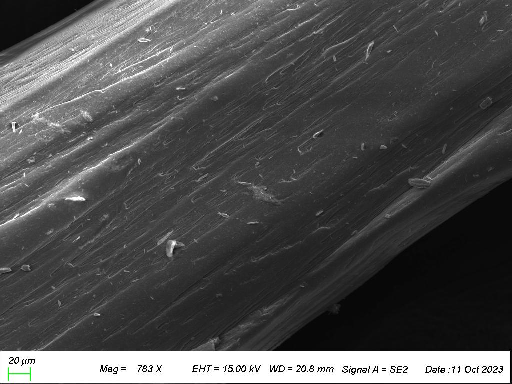
\includegraphics[width=0.46\textwidth]{bahiaGoeControl_20um4.pdf} &
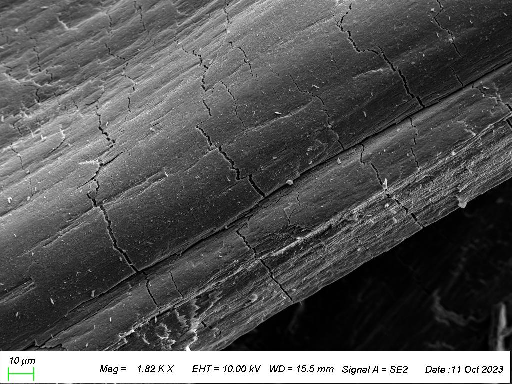
\includegraphics[width=0.46\textwidth]{Goethite_Vac_300C_11hr_10umB0.pdf} \\
\end{tabular}
\caption{Secondary electron images of Bahia goethite aggregate before heat treatment (control) and after heat treatment at 300\textdegree C for 11 hours in vacuum. Cracks developed in the vacuum-heated sample both parallel and perpendicular to the long axis of the polycrystalline aggregate, representing volume contraction due to dehydration/decomposition of goethite into hematite. The buffered treatments at the same temperature are shown in Fig.~\ref{fig:ch2-sem-buffered}.}
\label{fig:ch2-sem-control-vacuum}
\end{figure}

\begin{figure}[htbp]
\centering
\setlength{\tabcolsep}{4pt}
\begin{tabular}{cc}
\textbf{Gypsum-buffered, 300\textdegree C, 8 h} & \textbf{Water-buffered, 300\textdegree C, 4 h} \\[2pt]
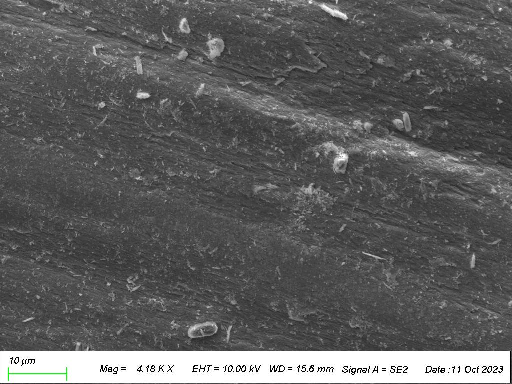
\includegraphics[width=0.46\textwidth]{bahiaGoeGypsum300C8hr_10um8.pdf} &
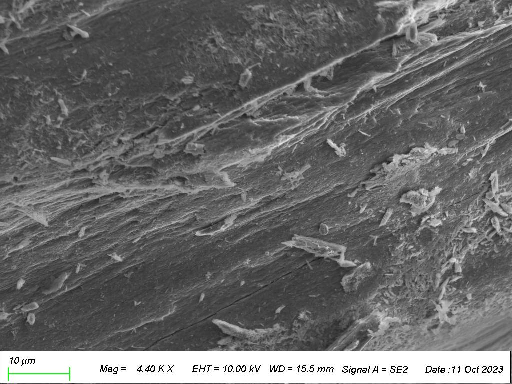
\includegraphics[width=0.46\textwidth]{Goeth_Water_300C_4hr_10um6.pdf} \\
\end{tabular}
\caption{Secondary electron images of Bahia goethite aggregate heated at 300\textdegree C in a sealed glass tube with gypsum (8 hours) and with water (4 hours). Despite treatment at high heat, no cracks indicative of dehydration were visible on either goethite surface. In the gypsum experiment, the gypsum dehydrated first and produced enough water pressure to stop or slow dehydration of the goethite and prevent the development of microscopic cracks; at higher temperatures goethite and gypsum reacted, forming a surface layer of other minerals. For the water-buffered sample, no cracks were observed when investigating the goethite at scales similar to Fig.~\ref{fig:ch2-sem-control-vacuum}, and most of the aggregate's surface resembled the gypsum-buffered panel; the area pictured had the roughest texture on the grain. A very small crack parallel to the long axis may indicate some amount of dehydration had occurred, or it could have been inherited from before hydrothermal treatment, since even the untreated control grain (Fig.~\ref{fig:ch2-sem-control-vacuum}) had some rough surfaces and rare long-axis-parallel cracks.}
\label{fig:ch2-sem-buffered}
\end{figure}

\begin{figure}[htbp]
\centering
\setlength{\tabcolsep}{4pt}
\begin{tabular}{cc}
\textbf{Vacuum, 300\textdegree C, 11 h (SE)} & \textbf{Vacuum, cross section (BSE)} \\[2pt]
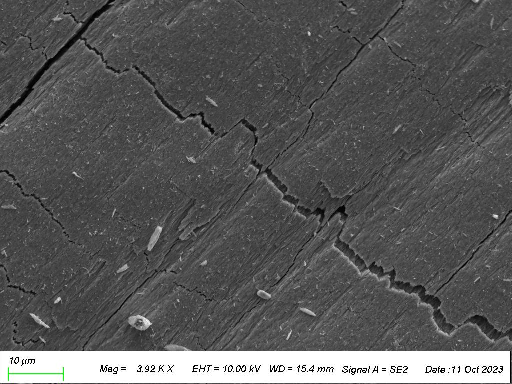
\includegraphics[width=0.46\textwidth]{Goethite_Vacuum_300C_11hr_10u9.pdf} &
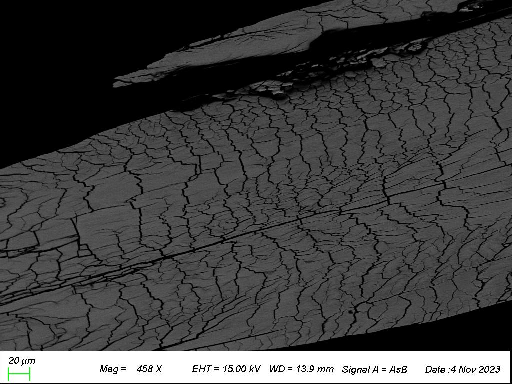
\includegraphics[width=0.46\textwidth]{C5_goeth_Vac205.pdf} \\
\end{tabular}
\caption{Vacuum-heated Bahia goethite at higher magnification and in cross section. Left: secondary electron image of goethite heated at 300\textdegree C for 11 hours in vacuum, at the same scale as the buffered samples of Fig.~\ref{fig:ch2-sem-buffered}, showing rough cracks at various scales both parallel and orthogonal to the long axis of the goethite aggregate. These are the typical decomposition features that would be expected in Fig.~\ref{fig:ch2-sem-buffered} if significant decomposition had occurred there. Right: backscatter electron image of a polished cross section of epoxy-mounted, vacuum-heated Bahia goethite, from the same subsample as the vacuum-heated grain of Fig.~\ref{fig:ch2-sem-control-vacuum}, exposing the grain's interior. This image clearly shows that the cracks visible on the exterior of dehydrated goethite are pervasive throughout the interior as well.}
\label{fig:ch2-sem-vacuum-interior}
\end{figure}

\section{Experimental Methods}\label{ch2-experimental-methods}

This study builds upon previous helium step heat studies of the dense
colloform goethite sample Win-06-01b (occasionally referred to as
Win0601b) collected within float at the Flinders Ranges in South
Australia \citep{waltenberg2012,monteiro2017}. It yields one of the
oldest known goethite U-Th/He ages: 180-135 Ma \citep{waltenberg2012}. To
produce a homogeneous distribution of 3He, Win-06-01b was irradiated
with 220 MeV protons for 24 hours at the Francis H. Burr Proton Therapy
Center, Massachusetts General Hospital, following standard procedures
\citep{shuster2005} and subsequently was subjected to helium step
heat measurements in vacuum by \citet{monteiro2017} and \citet{farley2024}.
In their step heat experiment of Win-06-01b, \citet{farley2024}
additionally measured evolved water using capacitance manometry to show
that helium and water release were tightly correlated for goethite step
heats in vacuum. Although they used subtly different heating schedules,
the results of \citet{farley2024} clearly agree well with \citet{monteiro2017}.

In this study, an aliquot of the same irradiated Win-06-01b goethite
used by \citet{monteiro2017} and \citet{farley2024} was encapsulated with
MilliQ water within a silica glass tube. Silica glass was chosen over
other laboratory glasses such as borosilicate because it is the most
permeable glass type to helium \citep{norton1953,altemose1961}. To
prepare the silica glass tube, 10 cm long segments of pure silica glass
tubes with an outer diameter of 4 mm and an inner diameter of 3 mm were
submerged and sonicated within acetone, ethanol, then MilliQ water baths
in sequence, and then were dried overnight in a 100°C oven. The glass
tubes were hand-pulled into thinner pipettes using a natural gas and
oxygen glass-welding torch and the pipette ends were fused closed. After
the glass had cooled, 1.18 mg of irradiated Win-06-01b goethite blades
less than 2 mm in length were carefully transferred to the bottom of the
tube in the presence of an ionizing fan. Less than a microliter of
distilled water was transferred to the sealed pipette using a thin glass
capillary, submerging the goethite, after which the tube was gently
tapped to liberate the bubbles and ensure that the water and goethite
were efficiently packed at the bottom of the pipette. To seal the
pipette, the contents of the ampoule were flash-frozen in liquid
nitrogen and transferred to a saltwater-ice bath at a temperature of
-10°C. While the pipette end of the tube remained frozen in the
saltwater-ice bath, the top was interfaced with a vacuum line and the
tube was pumped to a pressure of \textless0.1 torr. The advantage of
this approach was that water would remain solid within the tube, only
slowly sublimating to vacuum while atmospheric gasses would be readily
pumped away. While it was desirable to remove atmospheric gasses to
reduce experimental complexity by removing potentially reactive gasses
like oxygen, the primary motivation for pumping the tube to rough vacuum
was to aid the sealing process. When the tube contents were under
vacuum, fused glass would deform inwards and self-seal, greatly
improving the ease and quality of the seal while requiring far less heat
input from the torch. After an acceptably low pressure was attained, the
tube was closed to the vacuum line and the saltwater-ice bath was
quickly replaced with a liquid nitrogen bath, ensuring that no ice was
melted. The liquid nitrogen bath was preferable during sealing as it
more effectively protected the goethite and ice from the high
temperatures of the glass-welding torch. A fine-flamed welding torch was
used to seal the top of the ampoule, which dropped into the liquid
nitrogen bath and was retrieved by passing the liquid nitrogen through a
sieve. Fig.~\ref{fig:ch2-ampoule-post} shows the sealed ampoule after the completion of the
step heats with all of the original water remaining, a testament to the
quality of the ampoule's seal, which had sustained a massive pressure
gradient of over 11 orders of magnitude across the ampoule walls, with
an inner vapor pressure of about 3x10\textsuperscript{4} torr
(\textasciitilde40 bars: \citet{haar1984}) against the
\textasciitilde10\textsuperscript{-7} torr ultra-high vacuum of the lamp
cell while the ampoule was held at 250°C for over a week.

\begin{figure}[htbp]
\centering
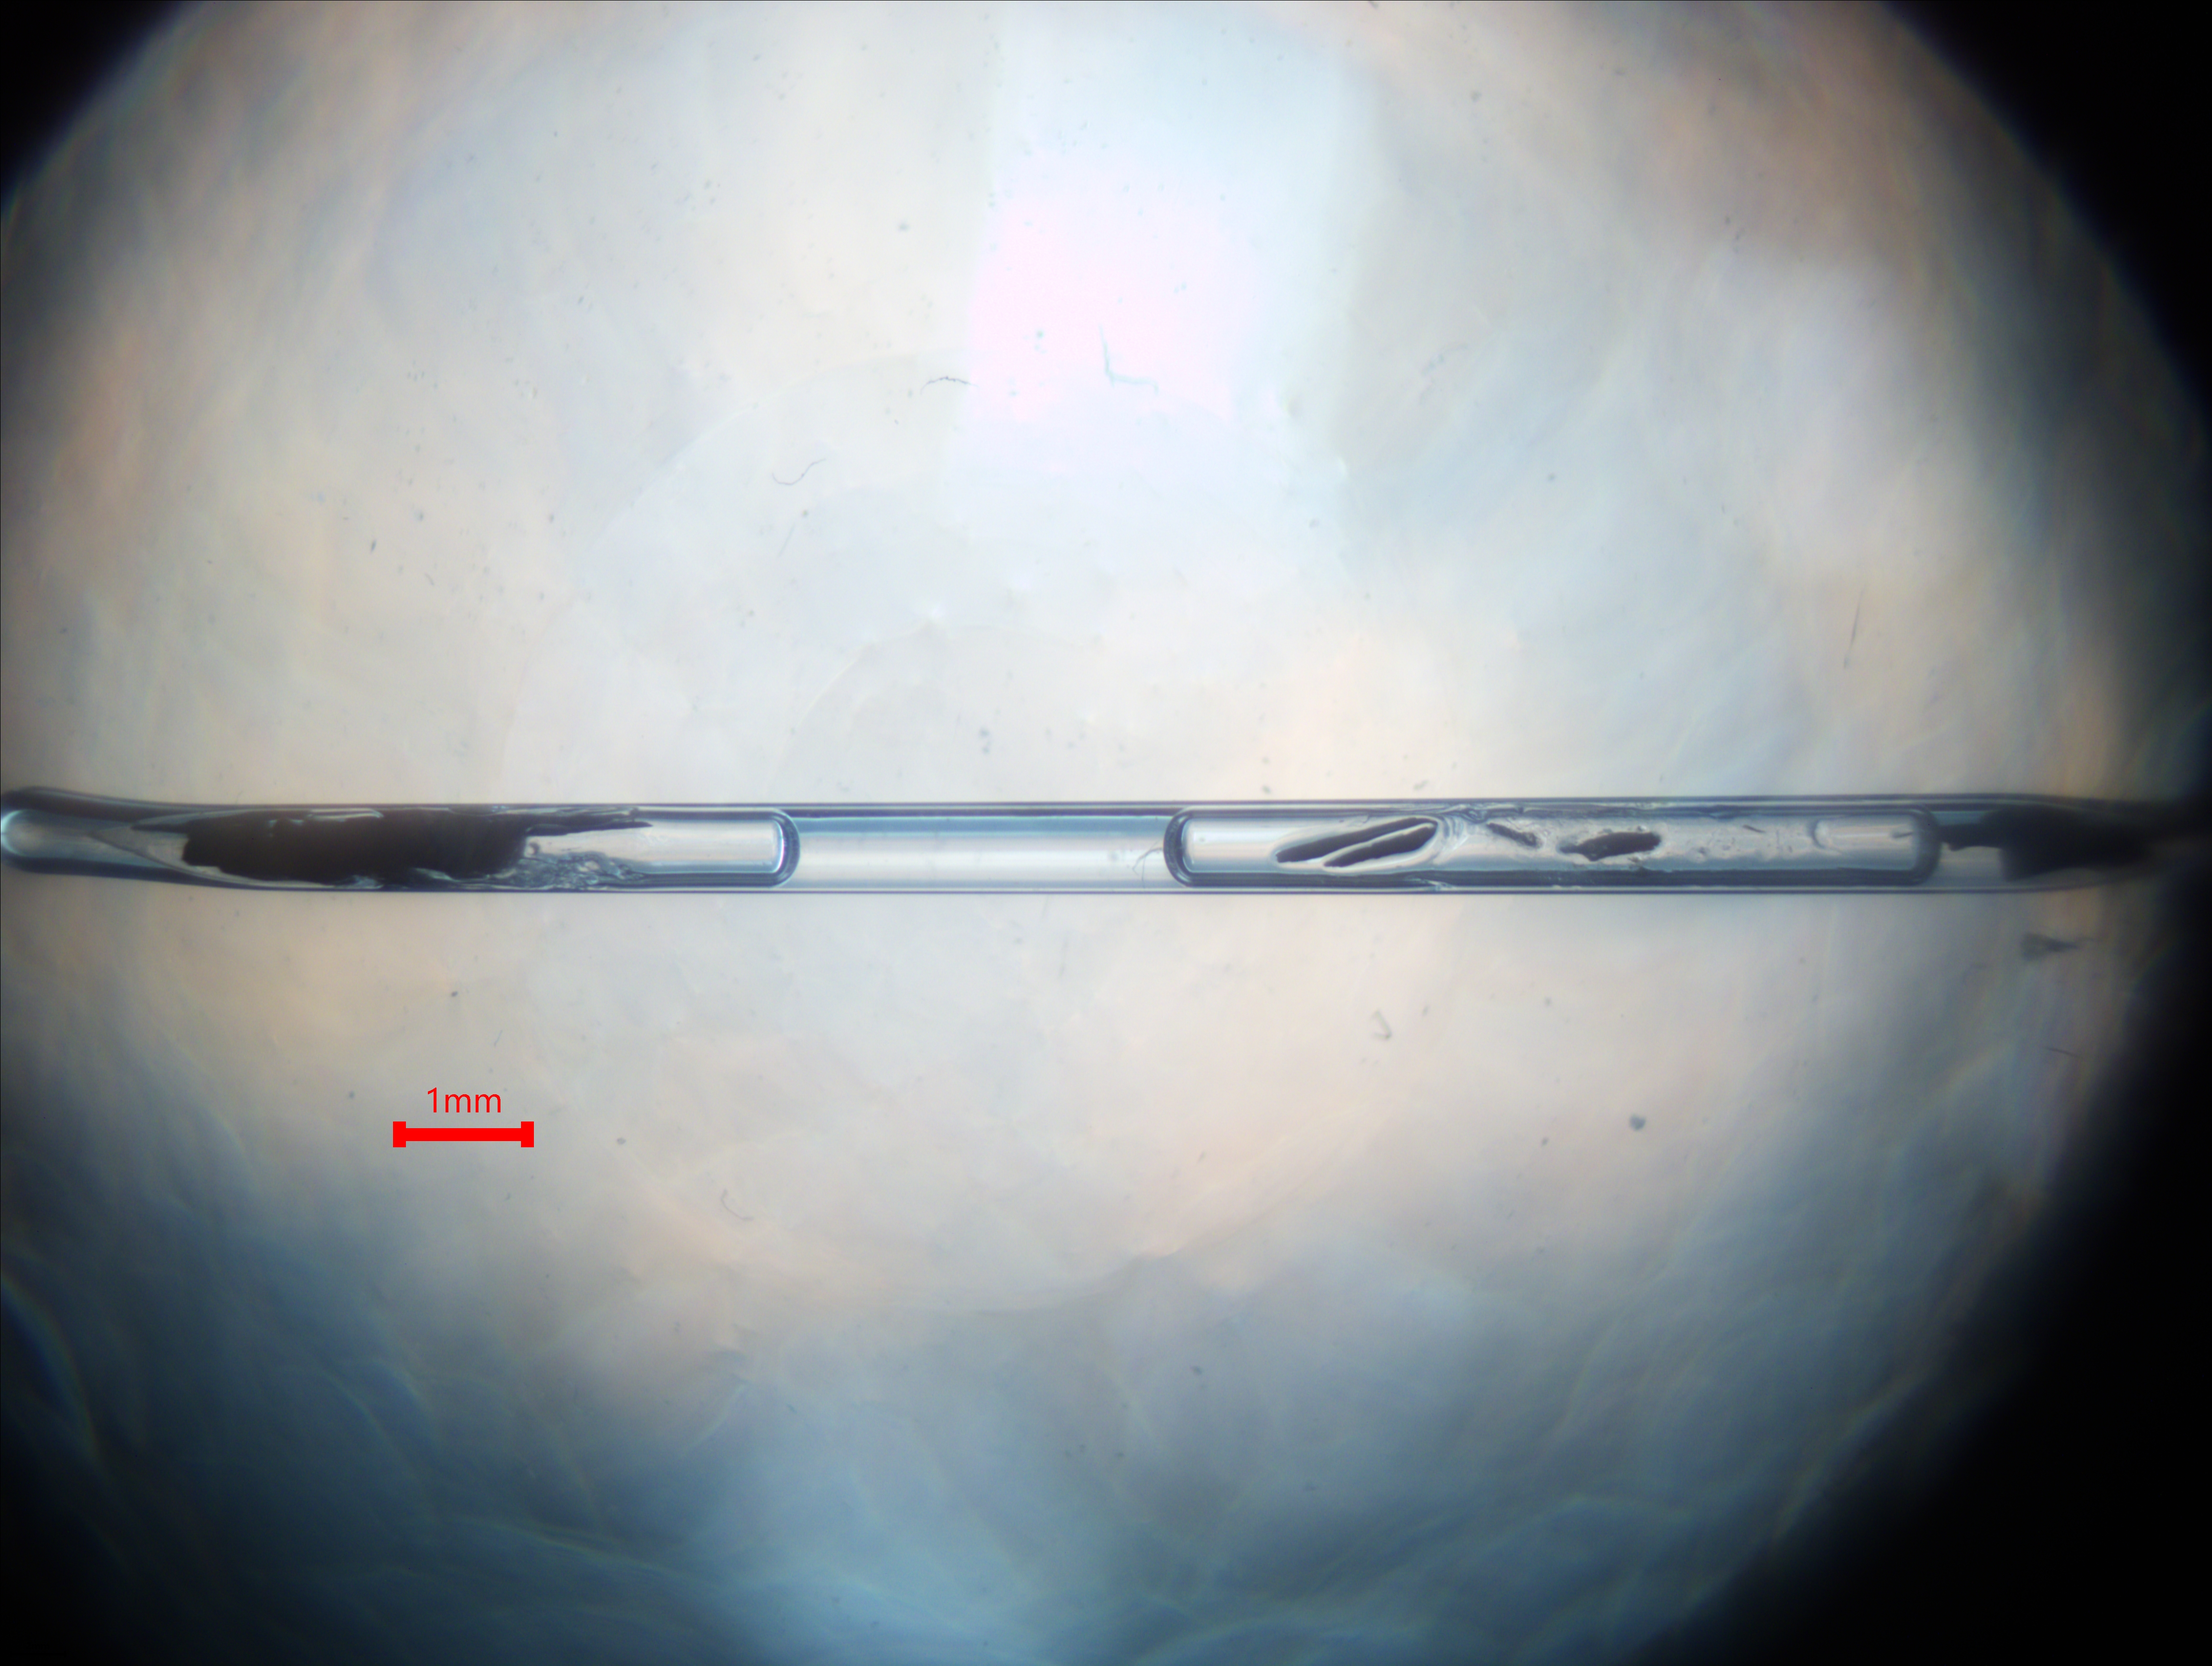
\includegraphics[width=0.7\textwidth]{zoomout2.jpg}
\caption{A view of the entire experimental ampoule after the completion of the step heat experiment before it was broken for the final step in the resistance furnace. At room temperature, the tube is approximately half-filled with gas, one-third filled with liquid water, and one-sixth filled with $<$2\,mm long shards of irradiated Win-06-01b goethite. A gel-like substance was observed lining the inner walls of the tube, which is likely to be amorphous silica dissolved from the tube and redeposited by the thermally-cycled, high pressure liquid water phase.}
\label{fig:ch2-ampoule-post}
\end{figure}

\begin{figure}[htbp]
\centering
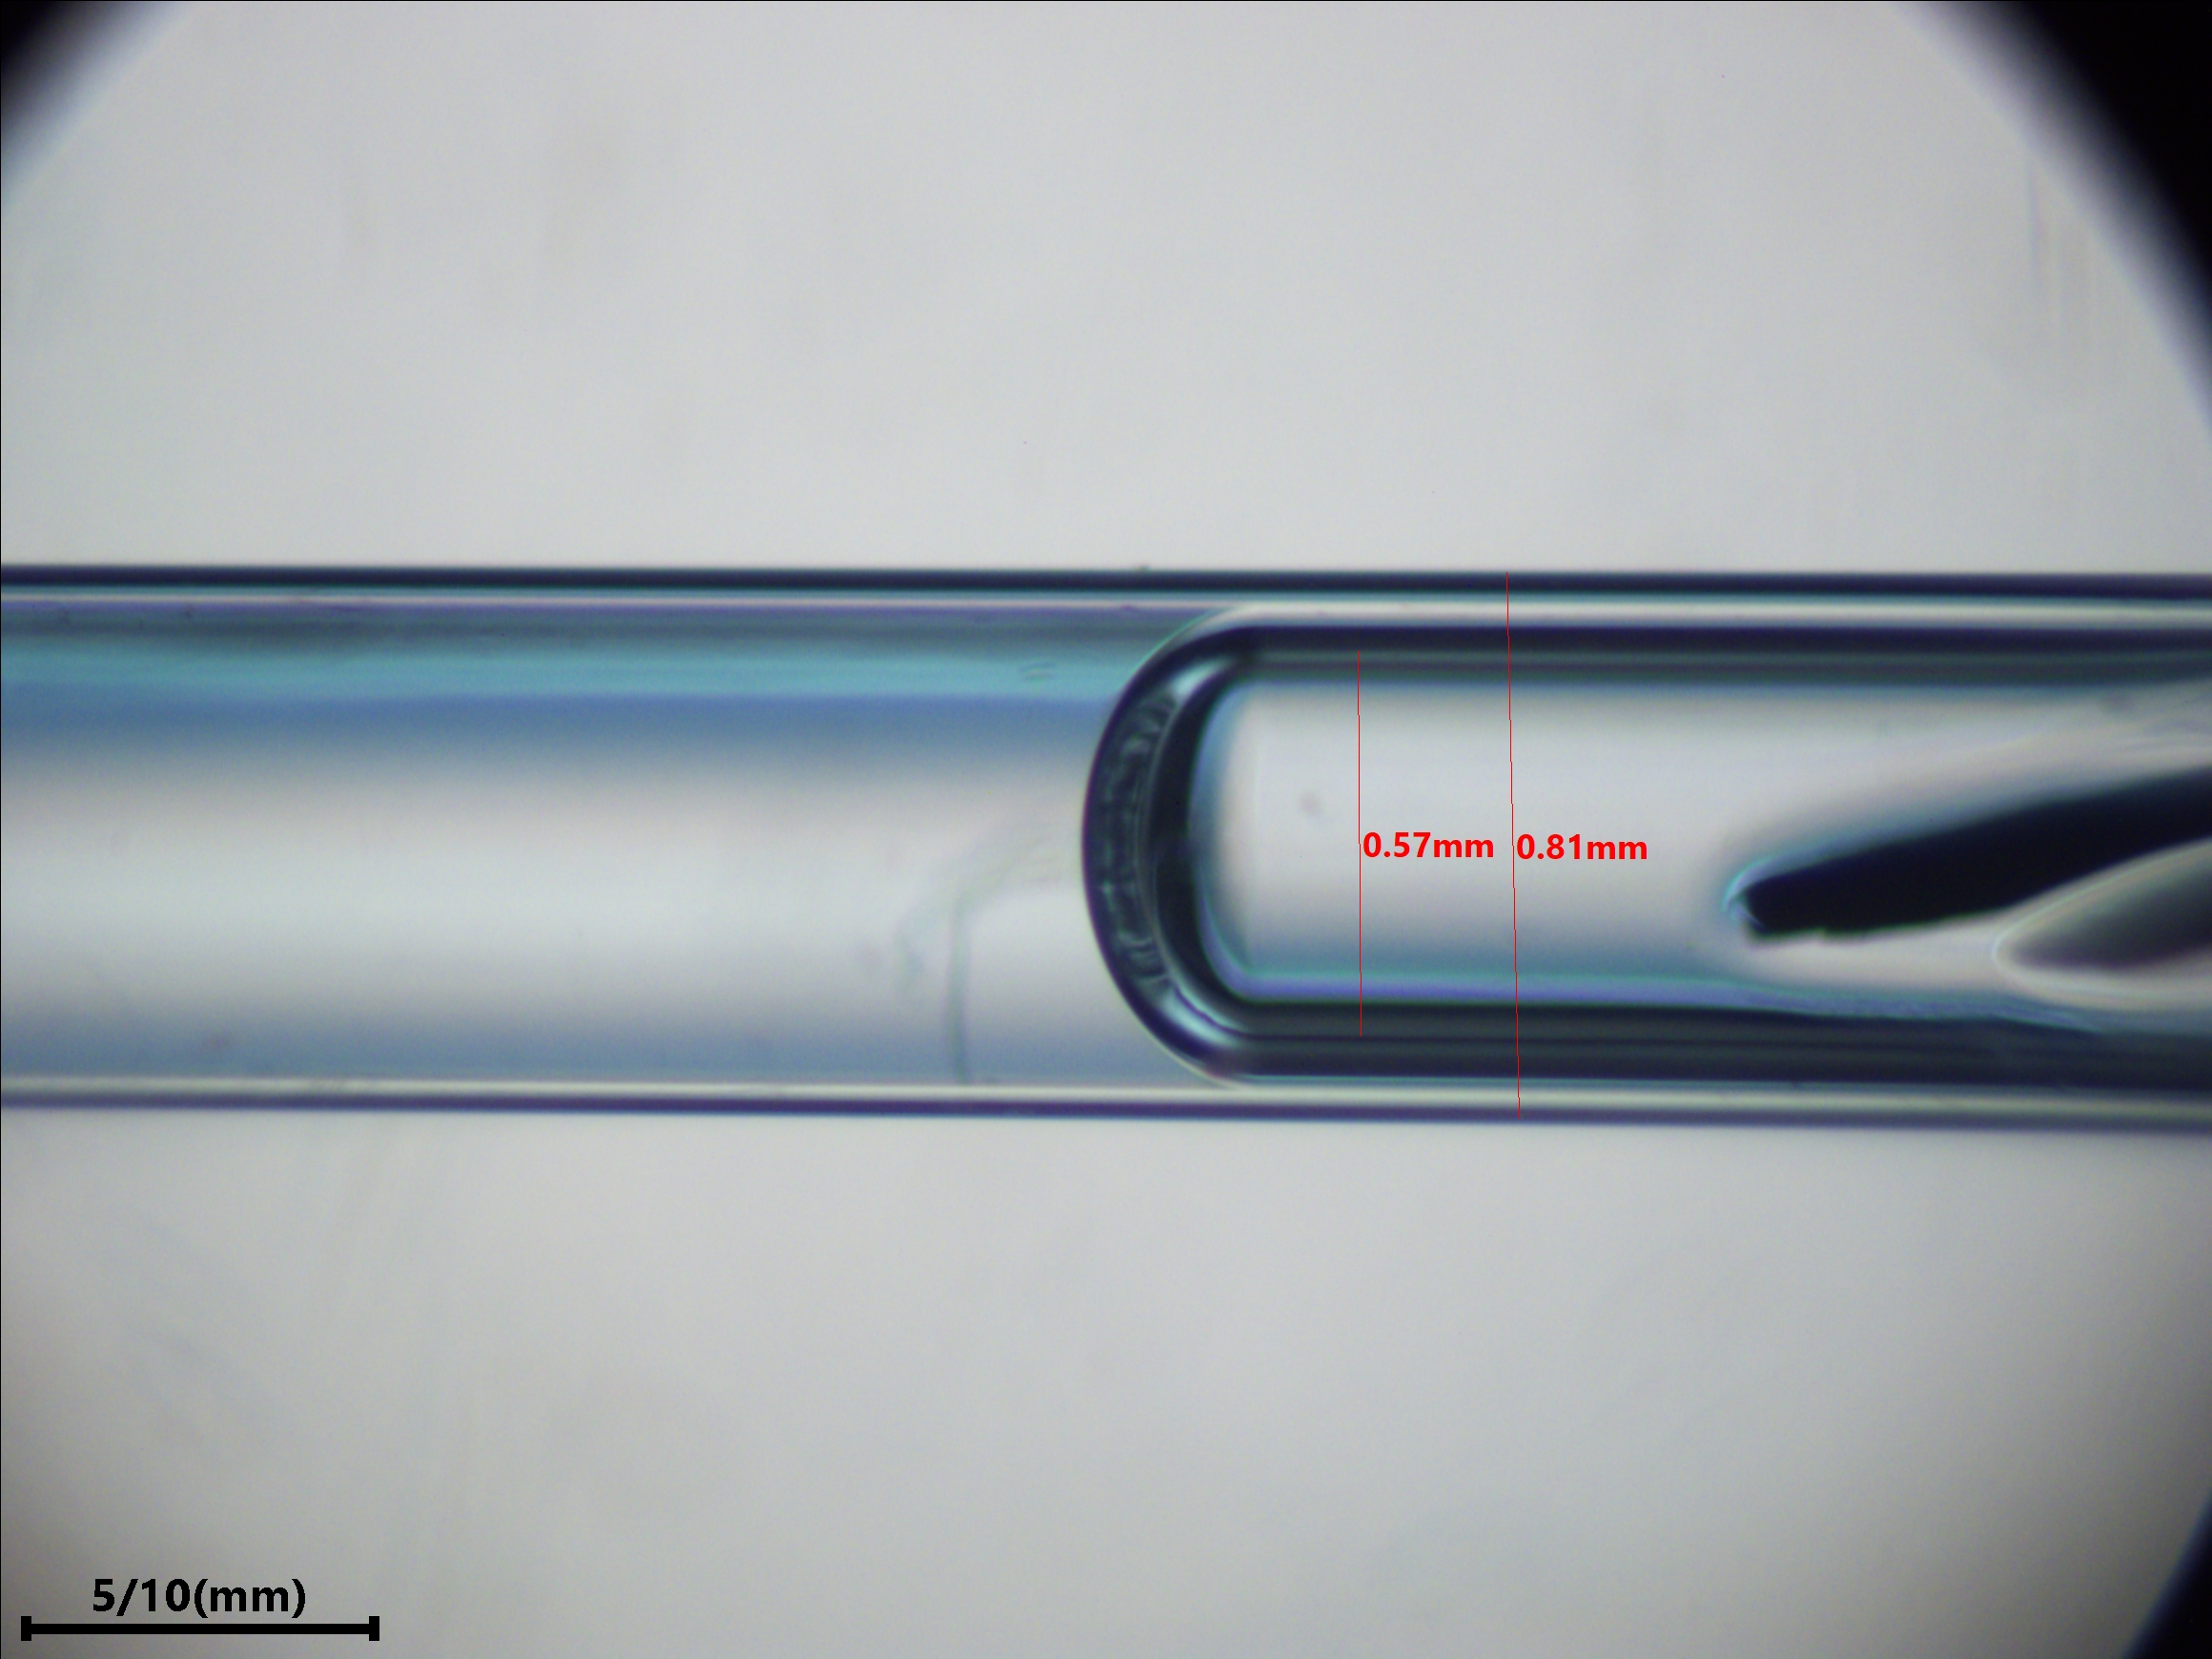
\includegraphics[width=0.7\textwidth]{measureGoeTube.jpg}
\caption{Measurements of the inner and outer diameter of the ampoule used in the hydrothermal step heats of Win-06-01b. The inner walls of the ampoule are only clearly visible within air bubbles.}
\label{fig:ch2-ampoule-dims}
\end{figure}

\clearpage


The sealed ampoule, now referred to as HT-Win-06-01b, was placed in a
copper foil packet and mounted to a K-type thermocouple within an
ultra-high vacuum projector lamp heating cell described in more detail
by \citet{farley1999}. Before the experiment began, the ampoule was
loaded in the lamp cell, pumped to high vacuum, and was held at 70°C for
4 days to degas atmospheric helium entrained within the ampoule.

HT-Win-06-01b was subjected to multiple prograde-retrograde heating
cycles to investigate possible MDD behavior. Step durations varied from
2 hours to about a week; the total experiment was conducted over about
40 days and included experimental steps ranging from 170-250°C. We
elected not to heat the sample hotter because high temperatures
generated very high vapor pressures. In early trials, we found that
similar ampoules most often withstood the \textasciitilde86 bar vapor
pressures associated with liquid water saturation at 300°C \citep{haar1984}, but they would explode when further heated to temperatures beyond
315°C.

Experimental temperature records show \textasciitilde1°C amplitude
oscillations around the target temperature. While we cannot exclude the
possibility that sustained temperature gradients were present throughout
the sample due to the use of the comparatively large \textasciitilde1 mm
thick ampoule, we are confident that the conclusions of this work are
robust. The ampoule was in direct contact with the thermocouple junction
and was in front of the thermocouple junction with respect to the projector
lamp heating source, suggesting that if there were a temperature
discrepancy, the sample would have been hotter than the recorded
temperature, which would not affect the conclusions of this work.
Additionally, during early trials of this method for helium step heats,
silica-glass encapsulated Durango apatite had been subjected to step
heats at Caltech and gave indistinguishable corrected 4He yields to
unencapsulated Durango apatite, suggesting that the temperature recorded
by the thermocouple for our experimental setup is sufficiently accurate.

Helium isotope measurements of evolved gasses from hydrothermal steps
heats of glass-encapsulated irradiated HT-Win-06-01b goethite were
acquired at Caltech on a Thermo Fisher
Helix-MC-Plus\textsuperscript{10K} mass spectrometer in peak hopping
mode from January 31\textsuperscript{st}, 2024 to March
13\textsuperscript{th}, 2024. Helium was purified by exposing evolved
gasses to a charcoal trap held in liquid nitrogen, a titanium sponge
getter, then a SAES NP10 getter before freely expanding into the
Helix-MC-Plus\textsuperscript{10K}. 3He was measured with a
pulse-counting electron multiplier, while 4He was detected on a Faraday
detector. The majority of the analysis time was spent measuring 3He.
Every few hours, the background was mass-scanned to set the 3He and 4He
measure points; each was taken to be a constant mass offset from the
background HD\textsuperscript{+} peak. These mass offsets are precisely
measured when tuning the Helix-MC-Plus\textsuperscript{10K} for helium
isotope analysis. Months of helium measurements with the
Helix-MC-Plus\textsuperscript{10K} at Caltech have shown this approach to
be reliable, reproducible, and accurate for helium isotope analysis.
Additionally, an electron multiplier monitored atomic mass 3.5 to detect
4He overspray, which was never significant during the experiment.
Measurements of high 3He MM gas standard were analyzed every 8 hours
(totaling 116 measurements) to track instrumental drift of 3He and 4He
sensitivities and to quantify internal reproducibility.

A cold blank was measured at the beginning of the experiment, showing a
negligible 3He blank essentially at 0 cps (technically this measurement
yielded a slightly negative intercept to time 0) and a 4He blank signal
corresponding to about 1.25 pccSTP, which was similar to 4He values
attained during low temperature permeation step measurements. Permeation
steps were thus assumed to measure shifting 4He blanks during the
experiment, and the entire blank correction was added to all 4He
uncertainties.

For the final step, the HT-Win-06-01b ampoule was broken and dried
overnight in a 50°C oven, then completely degassed by heating to
\textasciitilde1100 °C in a resistance furnace. The final step
measurement was conducted on a Thermo Fisher Helix SFT mass spectrometer. A
hot furnace blank subjected to the same volume splits as the final
HT-Win-06-01b measurement gave a 3He blank of 6.8 fccSTP and a 4He blank
of 0.31 nccSTP. This blank correction was less than 1\% of the measured
4He and negligible for 3He. A re-extract of HT-Win-06-01b immediately
following the measurement yielded above-blank 3He and 4He signals, which
were added to the total measurement, although both constituted less than
1\% of the final step yield. Sensitivity was calculated by measuring a
3He-enriched air standard with known 3He and 4He contents immediately
before the measurement.

Helium released by the sample reaches the mass spectrometer only after permeating the ampoule
wall, so each measured step yield lags the true release. Step yields were corrected for this
permeation lag with the bounding method of Chapter~\ref{ch:apparatus} (\S\ref{bounding-method}),
which gives lower-bound, central and upper-bound values for every step
(Tables~\ref{tab:ch2-distilled-3he} and~\ref{tab:ch2-distilled-4he}). The correction and the
ampoule permeabilities measured during the experiment are described in the Supplementary
Information (\S\ref{sec:ch2-si-permeation}), together with the diffusivity inversions, the
isotope-ratio uncertainties and the kinetic analysis of the published vacuum step heats
(\S\ref{ch2-analytical-methods}).

\paragraph{SEM Study of Thermally Treated Polycrystalline
Goethite}\label{sem-study-of-thermally-treated-polycrystalline-goethite}\label{sec:gt_pigment_methods}

In early trials of the ``glass tube method'' for helium step heat
experiments with controlled microenvironments presented here,
sub-samples of goethite morphologically similar to Win-06-01b from
Igarapé Bahia \citep{shustervasconcelos2005,monteiro2017} were heated in
vacuum using the projector lamp heating apparatus of \citet{farley1999}
and in sealed glass ampoules with gypsum or water additionally added to
provide moisture to slow/prevent dehydration of goethite. All samples
were held at 300°C for 4-11 hours, and the glass ampoules were broken
and the goethites were allowed to air dry before all samples were placed
on carbon tape and carbon coated. These samples were imaged at Caltech
on Secondary Electron mode by the ZEISS 1550VP Field Emission SEM.
Synthetic goethite pigment, a commercial yellow iron-oxide pigment of acicular crystals
$\sim$1~\textmu m long, was treated in the same way but only with water, without vacuum or
open-air runs: at least five larger silica glass ampoules, each loaded with pigment and an excess
of water and fused shut at ambient pressure, were held at 200--250~$^\circ$C for about a day in an
oven whose voltage was adjusted by hand. These runs were a rapid, qualitative test; details of
individual runs (temperature histories, durations, water-to-solid ratios) were not recorded, and
reaction was assessed by color (yellow goethite, red hematite) before imaging.
% TODO: add the pigment product name/grade and supplier; confirm SEM instrument/sample
% preparation for the pigment images (SE2, 10 kV, Feb 2024).

\section{\texorpdfstring{Results }{Results }}\label{ch2-results}

The complete corrected step-heat dataset underlying the diffusivities, delta plots, and Arrhenius regressions discussed below is distilled in Tables~\ref{tab:ch2-distilled-3he} and~\ref{tab:ch2-distilled-4he}, reporting the lower-bound, central, and upper-bound values from the bounding method's permeation-lag correction for $^3$He and $^4$He respectively.

\begin{landscape}
\begin{footnotesize}
\begin{longtable}{r r r r r r r r r r}
\caption{$^3$He step-heat dataset for HT-Win-06-01b under the bounding method: measured and cumulative $^3$He, the upper-bound residual ampoule content ($n_{t,\mathrm{UB}}$), the lower- and upper-bound true step production ($\omega_{\mathrm{LB}}$, $\omega_{\mathrm{UB}}$), and the corresponding lower-bound, central, and upper-bound apparent diffusivities. ``--'' denotes early steps with $\lambda t < 4$, for which bounds could not be determined (see \S\ref{permeation-lag-correction}). Six rows have derived values marked with ``*'': these steps have measured $^3$He $<0.1$ pccSTP and are excluded as low-signal from all plots (Fig.~\ref{fig:ch2-ratio-spectra} and others derived from this dataset).}\label{tab:ch2-distilled-3he}\\
\toprule
Temp & Time & $^3$He meas. & Cum. $^3$He & $n_{t,\mathrm{UB}}$ & $\omega_{\mathrm{LB}}$ & $\omega_{\mathrm{UB}}$ & $\ln(D/a^2)_{\mathrm{LB}}$ & $\ln(D/a^2)_{m}$ & $\ln(D/a^2)_{\mathrm{UB}}$ \\
(°C) & (min) & (pccSTP) & (pccSTP) & (pccSTP) & (pccSTP) & (pccSTP) &  &  &  \\
\midrule
\endfirsthead
\multicolumn{10}{l}{\textit{(continued)}} \\
\toprule
Temp & Time & $^3$He meas. & Cum. $^3$He & $n_{t,\mathrm{UB}}$ & $\omega_{\mathrm{LB}}$ & $\omega_{\mathrm{UB}}$ & $\ln(D/a^2)_{\mathrm{LB}}$ & $\ln(D/a^2)_{m}$ & $\ln(D/a^2)_{\mathrm{UB}}$ \\
(°C) & (min) & (pccSTP) & (pccSTP) & (pccSTP) & (pccSTP) & (pccSTP) &  &  &  \\
\midrule
\endhead
\midrule
\multicolumn{10}{r}{\textit{continued on next page}} \\
\endfoot
\bottomrule
\endlastfoot
170 & 300 & 0.9630 & 0.0000 & 1.1660 & -- & -- & -- & -- & -- \\
180 & 463 & 0.5442 & 0.9630 & 0.2413 & -- & -- & -- & -- & -- \\
190 & 550 & 0.5292 & 1.6241 & 0.1538 & -- & -- & -- & -- & -- \\
200 & 500 & 0.5190 & 2.2112 & 0.1430 & 0.3651 & 0.6619 & -22.158 & -21.775 & -21.503 \\
210 & 475 & 0.5770 & 2.7646 & 0.1440 & 0.4341 & 0.7210 & -21.715 & -21.406 & -21.160 \\
220 & 450 & 0.6333 & 3.3799 & 0.1447 & 0.4894 & 0.7781 & -21.345 & -21.068 & -20.843 \\
230 & 425 & 0.7899 & 4.0551 & 0.1685 & 0.6452 & 0.9584 & -20.823 & -20.604 & -20.392 \\
225 & 908 & 0.7513 & 4.8885 & 0.0716 & 0.5827 & 0.8229 & -21.516 & -21.246 & -21.148 \\
215 & 450 & 0.1415 & 5.6842 & 0.0349 & 0.0699 & 0.1764 & -22.836 & -22.124 & -21.900 \\
205 & 520 & 0.0763 & 5.8529 & 0.0184$^*$ & 0.0413$^*$ & 0.0947$^*$ & -23.479$^*$ & -22.863$^*$ & -22.646$^*$ \\
195 & 1106 & 0.0670 & 5.9491 & 0.0080$^*$ & 0.0487$^*$ & 0.0750$^*$ & -24.053$^*$ & -23.731$^*$ & -23.618$^*$ \\
185 & 740 & 0.0227 & 6.0246 & 0.0049$^*$ & 0.0147$^*$ & 0.0276$^*$ & -24.839$^*$ & -24.404$^*$ & -24.207$^*$ \\
175 & 920 & 0.0180 & 6.0610 & 0.0036$^*$ & 0.0131$^*$ & 0.0216$^*$ & -25.168$^*$ & -24.847$^*$ & -24.665$^*$ \\
200 & 260 & 0.0224 & 6.0814 & 0.0163$^*$ & 0.0189$^*$ & 0.0388$^*$ & -23.534$^*$ & -23.360$^*$ & -22.812$^*$ \\
210 & 520 & 0.0812 & 6.1081 & 0.0181$^*$ & 0.0649$^*$ & 0.0993$^*$ & -22.984$^*$ & -22.758$^*$ & -22.554$^*$ \\
220 & 1167 & 0.5766 & 6.1914 & 0.0447 & 0.5585 & 0.6213 & -21.587 & -21.553 & -21.475 \\
230 & 370 & 0.3577 & 6.7796 & 0.0903 & 0.3130 & 0.4480 & -20.948 & -20.811 & -20.579 \\
240 & 320 & 0.6767 & 7.1563 & 0.1776 & 0.5864 & 0.8543 & -20.062 & -19.913 & -19.667 \\
245 & 250 & 0.5549 & 7.8582 & 0.1888 & 0.3773 & 0.7437 & -20.176 & -19.778 & -19.474 \\
250 & 210 & 0.6934 & 8.4743 & 0.2786 & 0.5047 & 0.9721 & -19.626 & -19.296 & -18.942 \\
245 & 270 & 0.4659 & 9.2086 & 0.1413 & 0.1872 & 0.6071 & -20.801 & -19.874 & -19.601 \\
240 & 320 & 0.2857 & 9.7206 & 0.0749 & 0.1445 & 0.3606 & -21.176 & -20.487 & -20.250 \\
235 & 370 & 0.2199 & 10.0357 & 0.0517 & 0.1450 & 0.2716 & -21.284 & -20.864 & -20.650 \\
230 & 420 & 0.1400 & 10.2736 & 0.0303 & 0.0883 & 0.1703 & -21.885 & -21.421 & -21.224 \\
225 & 652 & 0.1494 & 10.4279 & 0.0206 & 0.1191 & 0.1700 & -22.009 & -21.781 & -21.650 \\
230 & 500 & 0.1550 & 10.5908 & 0.0271 & 0.1344 & 0.1820 & -21.605 & -21.462 & -21.299 \\
235 & 450 & 0.1951 & 10.7582 & 0.0361 & 0.1681 & 0.2313 & -21.258 & -21.107 & -20.936 \\
240 & 400 & 0.2425 & 10.9638 & 0.0483 & 0.2063 & 0.2908 & -20.913 & -20.750 & -20.566 \\
245 & 350 & 0.3150 & 11.2328 & 0.0690 & 0.2667 & 0.3840 & -20.495 & -20.326 & -20.125 \\
250 & 300 & 0.3716 & 11.5689 & 0.0939 & 0.3026 & 0.4656 & -20.181 & -19.973 & -19.743 \\
250 & 300 & 0.3640 & 11.9627 & 0.0899 & 0.2700 & 0.4539 & -20.261 & -19.959 & -19.734 \\
250 & 300 & 0.3452 & 12.3490 & 0.0852 & 0.2553 & 0.4304 & -20.285 & -19.979 & -19.755 \\
250 & 10250 & 8.4829 & 12.7167 & 0.0494 & 8.3977 & 8.5324 & -19.989 & -19.976 & -19.969 \\
240 & 785 & 0.2261 & 21.2187 & 0.0209 & 0.1767 & 0.2470 & -21.026 & -20.778 & -20.689 \\
\midrule
\textbf{Total} &  &  & 146.1483 &  &  &  &  &  &  \\
\end{longtable}
\end{footnotesize}
\end{landscape}

\begin{landscape}
\begin{footnotesize}
\begin{longtable}{r r r r r r r r r r r r r}
\caption{$^4$He step-heat dataset and absolute $^4$He/$^3$He ratios for HT-Win-06-01b under the bounding method, structured as in Table~\ref{tab:ch2-distilled-3he}. ``--'' denotes steps for which bounds could not be determined. The Total row reports the bulk (total-yield) $^4$He/$^3$He ratio, i.e. the normalizing value used to bulk-normalize these ratios for the plot in Fig.~\ref{fig:ch2-ratio-spectra}. Six rows have derived values marked with ``*'': these steps have measured $^3$He $<0.1$ pccSTP and are excluded as low-signal from all plots, as in Table~\ref{tab:ch2-distilled-3he}.}\label{tab:ch2-distilled-4he}\\
\toprule
Temp & Time & $^4$He meas. & Cum. $^4$He & $n_{t,\mathrm{UB}}$ & $\omega_{\mathrm{LB}}$ & $\omega_{\mathrm{UB}}$ & $\ln(D/a^2)_{\mathrm{LB}}$ & $\ln(D/a^2)_{m}$ & $\ln(D/a^2)_{\mathrm{UB}}$ & $(^4\mathrm{He}/^3\mathrm{He})_{\mathrm{LB}}$ & $(^4\mathrm{He}/^3\mathrm{He})_{m}$ & $(^4\mathrm{He}/^3\mathrm{He})_{\mathrm{UB}}$ \\
(°C) & (min) & (nccSTP) & (nccSTP) & (nccSTP) & (nccSTP) & (nccSTP) &  &  &  &  &  &  \\
\midrule
\endfirsthead
\multicolumn{13}{l}{\textit{(continued)}} \\
\toprule
Temp & Time & $^4$He meas. & Cum. $^4$He & $n_{t,\mathrm{UB}}$ & $\omega_{\mathrm{LB}}$ & $\omega_{\mathrm{UB}}$ & $\ln(D/a^2)_{\mathrm{LB}}$ & $\ln(D/a^2)_{m}$ & $\ln(D/a^2)_{\mathrm{UB}}$ & $(^4\mathrm{He}/^3\mathrm{He})_{\mathrm{LB}}$ & $(^4\mathrm{He}/^3\mathrm{He})_{m}$ & $(^4\mathrm{He}/^3\mathrm{He})_{\mathrm{UB}}$ \\
(°C) & (min) & (nccSTP) & (nccSTP) & (nccSTP) & (nccSTP) & (nccSTP) &  &  &  &  &  &  \\
\midrule
\endhead
\midrule
\multicolumn{13}{r}{\textit{continued on next page}} \\
\endfoot
\bottomrule
\endlastfoot
170 & 300 & 0.0192 & 0.0000 & 0.0280 & -- & -- & -- & -- & -- & -- & -- & -- \\
180 & 463 & 0.0305 & 0.0192 & 0.0152 & -- & -- & -- & -- & -- & -- & -- & -- \\
190 & 550 & 0.0558 & 0.0660 & 0.0179 & -- & -- & -- & -- & -- & -- & -- & -- \\
200 & 500 & 0.1024 & 0.1375 & 0.0313 & 0.0845 & 0.1337 & -26.207 & -25.965 & -25.619 & -- & 197.3 & -- \\
210 & 475 & 0.1460 & 0.2500 & 0.0404 & 0.1147 & 0.1864 & -25.314 & -25.022 & -24.717 & 248.2 & 253.0 & 268.8 \\
220 & 450 & 0.2091 & 0.4055 & 0.0530 & 0.1686 & 0.2620 & -24.407 & -24.152 & -23.876 & 326.3 & 330.1 & 349.3 \\
230 & 425 & 0.3243 & 0.6319 & 0.0760 & 0.2714 & 0.4004 & -23.425 & -23.213 & -22.956 & 403.7 & 410.6 & 432.3 \\
225 & 908 & 0.3483 & 0.9799 & 0.0363 & 0.2722 & 0.3845 & -23.807 & -23.527 & -23.413 & 442.6 & 463.6 & 474.4 \\
215 & 450 & 0.0716 & 1.3487 & 0.0196 & 0.0353 & 0.0912 & -24.945 & -24.225 & -23.976 & 429.1 & 505.9 & 537.1 \\
205 & 520 & 0.0385 & 1.4359 & 0.0103$^*$ & 0.0189$^*$ & 0.0487$^*$ & -25.661$^*$ & -24.942$^*$ & -24.701$^*$ & 392.4$^*$ & 504.2$^*$ & 534.6$^*$ \\
195 & 1106 & 0.0336 & 1.4912 & 0.0043$^*$ & 0.0233$^*$ & 0.0379$^*$ & -26.165$^*$ & -25.796$^*$ & -25.675$^*$ & 446.7$^*$ & 500.9$^*$ & 515.3$^*$ \\
185 & 740 & 0.0079 & 1.5467 & 0.0019$^*$ & 0.0037$^*$ & 0.0098$^*$ & -27.586$^*$ & -26.808$^*$ & -26.592$^*$ & 224.7$^*$ & 350.1$^*$ & 369.1$^*$ \\
175 & 920 & 0.0152 & 1.6020 & 0.0033$^*$ & 0.0133$^*$ & 0.0185$^*$ & -26.475$^*$ & -26.340$^*$ & -26.141$^*$ & 843.2$^*$ & 843.2$^*$ & 982.0$^*$ \\
200 & 260 & 0.0107 & 1.6351 & 0.0091$^*$ & 0.0073$^*$ & 0.0198$^*$ & -25.787$^*$ & -25.411$^*$ & -24.791$^*$ & 375.6$^*$ & 475.5$^*$ & 554.7$^*$ \\
210 & 520 & 0.2166 & 1.6547 & 0.0535$^*$ & 0.2075$^*$ & 0.2701$^*$ & -23.067$^*$ & -23.021$^*$ & -22.786$^*$ & 2667.1$^*$ & 2667.1$^*$ & 3103.8$^*$ \\
220 & 1167 & 0.3187 & 1.8714 & 0.0269 & 0.2652 & 0.3456 & -23.499 & -23.302 & -23.214 & 471.7 & 552.7 & 563.2 \\
230 & 370 & 0.2113 & 2.6766 & 0.0590 & 0.1844 & 0.2703 & -22.391 & -22.249 & -21.993 & 575.1 & 590.8 & 628.0 \\
240 & 320 & 0.4286 & 3.1616 & 0.1243 & 0.3697 & 0.5529 & -21.360 & -21.203 & -20.931 & 612.1 & 633.4 & 674.8 \\
245 & 250 & 0.3988 & 3.6430 & 0.1521 & 0.2746 & 0.5510 & -21.289 & -20.899 & -20.556 & 665.9 & 718.7 & 778.4 \\
250 & 210 & 0.4440 & 4.2359 & 0.2020 & 0.2918 & 0.6460 & -20.906 & -20.469 & -20.072 & 541.7 & 640.2 & 702.8 \\
245 & 270 & 0.3123 & 4.7263 & 0.1053 & 0.1103 & 0.4176 & -22.043 & -20.981 & -20.680 & 469.1 & 670.4 & 721.4 \\
240 & 320 & 0.1927 & 5.0846 & 0.0559 & 0.0874 & 0.2485 & -22.376 & -21.575 & -21.315 & 505.5 & 674.3 & 718.4 \\
235 & 370 & 0.1517 & 5.3031 & 0.0393 & 0.0958 & 0.1910 & -22.386 & -21.922 & -21.688 & 599.8 & 689.6 & 729.9 \\
230 & 420 & 0.0991 & 5.4714 & 0.0236 & 0.0598 & 0.1227 & -22.956 & -22.448 & -22.232 & 608.3 & 707.9 & 745.9 \\
225 & 652 & 0.0995 & 5.5835 & 0.0151 & 0.0760 & 0.1146 & -23.136 & -22.863 & -22.721 & 608.2 & 666.5 & 689.2 \\
230 & 500 & 0.1051 & 5.6969 & 0.0202 & 0.0900 & 0.1253 & -22.679 & -22.523 & -22.345 & 652.1 & 678.1 & 707.5 \\
235 & 450 & 0.1369 & 5.8251 & 0.0279 & 0.1167 & 0.1648 & -22.290 & -22.128 & -21.940 & 674.6 & 701.7 & 734.0 \\
240 & 400 & 0.1781 & 5.9762 & 0.0390 & 0.1502 & 0.2171 & -21.892 & -21.719 & -21.518 & 705.1 & 734.6 & 770.9 \\
245 & 350 & 0.2305 & 6.1807 & 0.0556 & 0.1915 & 0.2861 & -21.479 & -21.290 & -21.070 & 694.4 & 731.9 & 771.7 \\
250 & 300 & 0.2777 & 6.4385 & 0.0758 & 0.2221 & 0.3535 & -21.134 & -20.906 & -20.659 & 703.3 & 747.3 & 793.3 \\
250 & 300 & 0.2654 & 6.7374 & 0.0725 & 0.1896 & 0.3379 & -21.250 & -20.908 & -20.661 & 653.7 & 729.2 & 774.1 \\
250 & 300 & 0.2489 & 7.0231 & 0.0680 & 0.1764 & 0.3169 & -21.282 & -20.932 & -20.647 & 646.8 & 721.0 & 765.4 \\
250 & 10250 & 6.8042 & 7.2901 & 0.0430 & 6.7362 & 6.8472 & -20.704 & -20.691 & -20.682 & 800.6 & 802.1 & 803.3 \\
240 & 785 & 0.1853 & 14.1156 & 0.0187 & 0.1423 & 0.2040 & -21.688 & -21.422 & -21.325 & 770.5 & 819.4 & 838.0 \\
\midrule
\textbf{Total} &  &  & 145.8145 &  &  &  &  &  &  &  & 997.7 &  \\
\end{longtable}
\end{footnotesize}
\end{landscape}


The diffusivities determined from the corrected step heat 3He and 4He
yields for HT-Win-06-01b are always significantly lower than the
diffusivities determined from step heat experiments on the same sample
in vacuum, and evolutions that are distinct from those determined from
the vacuum experiments. The Arrhenius plot of the 3He diffusivities
initially follow a declining concave-up trend until \textasciitilde3.5\%
cumulative 3He yield, then slowly decreasing in sub-parallel arrays
during prograde and retrograde heating cycles from 3.5-7\% cumulative
3He yields (Fig.~\ref{fig:ch2-arrhenius-zoom}, Fig.~\ref{fig:ch2-delta-zoom}). The Arrhenius plot of the 4He diffusivities
differs in shape: it is concave-down to about 5\% cumulative 3He yield,
after which it follows a roughly linear array about one log unit below
the 3He array (Fig.~\ref{fig:ch2-arrhenius-zoom}). The 3He diffusivities settled into a
linear array which was suitable for linear regression after
\textasciitilde7\% of the cumulative 3He yield was lost (Fig.~\ref{fig:gt_arrhenius}b). All
remaining diffusivity measurements of the experiment were included in
the linear regression, so that diffusivities from 3He loss fractions of
about 7-15\% were included. The linear regression yields an
R\textsuperscript{2} of \ChTwoRtwo, an activation energy of \ChTwoEa ± \ChTwoEaErr
kJ/mol, and a closure temperature of \ChTwoTc ± \ChTwoTcErr °C assuming a cooling
rate of 10°C/Ma and considering only the uncertainty in the regression
intercept (D\textsubscript{0}/a\textsuperscript{2}).
\begin{figure}[htbp]
\centering
\includegraphics[width=\textwidth]{arrhenius_reaction_vs_diffusion.pdf}
\caption{The $^3$He release of every step of the two vacuum step heats of Win-06-01b (red circles:
KAF, \citealt{farley2024}; orange squares: HDM, \citealt{monteiro2017}) and of the hydrothermal
step heat of this study (blue diamonds), reduced in two ways: (a) as first-order conversion rate
constants $k_i$ (Eq.~\eqref{eq:gt_stepk}, $\phi=\ChTwoKinPhi$), and (b) as \citet{fechtigkalbitzer1966}
apparent diffusivities $D/a^2$ for a sphere (Eq.~\eqref{eq:gt_FK}). The points of each experiment
are joined in step order by dashed lines. Filled vacuum symbols are the steps in the kinetic fitting
window and open symbols lie outside it; large pink circles mark the two KAF steps with the
LN$_2$ trap isolated. Hydrothermal steps are bounding-method central values, with bars spanning the
lower and upper bounds; low-signal steps are excluded. Black line: joint first-order Arrhenius fit
to the KAF and HDM steps in the window (Eq.~\eqref{eq:gt_line}). The two reductions give the
experiments opposite geometries. For the vacuum step heats, the first-order reduction collapses
both heating schedules onto one line, including the retrograde steps of HDM, whereas the diffusion
reduction separates the schedules, places HDM's retrograde steps above its own prograde steps and
turns over above $\sim$275~$^\circ$C as release stalls at the hematite plateau, none of which a
depleting diffusion domain can produce. For the hydrothermal step heat the pattern reverses. As rate
constants, its steps sit 1.3--2.8 orders of magnitude below the vacuum line and split into
history-dependent arrays that first-order kinetics forbids, with retrograde steps below prograde
steps at the same temperature. As diffusivities, the same steps form a single coherent array,
approximately seven natural-log units below the vacuum values, whose offsets through the temperature
cycles follow the depletion of the least retentive domains (\S\ref{sec:gt_hydro}). Below
$\sim$180~$^\circ$C both vacuum experiments depart from the first-order line, reflecting a small,
separate low-temperature component (\S\ref{sec:gt_vacuum}). Steps with $F>1-\phi$ have no defined
$k$ and are absent from (a).}
\label{fig:gt_arrhenius}
\end{figure}

\begin{figure}[htbp]
\centering
\includegraphics[width=0.8\textwidth]{winsor_goethite_Diffusivities_Arrhenius_Zoomin.pdf}
\caption{Linear regression of the last \ChTwoN\ measurements of 3He diffusivities in HT-Win-06-01b defining the ``Stage 1'' reference line. Apparent diffusivities under hydrothermal conditions are approximately seven natural log units lower than in vacuum. A diffusion domain corresponding to the Stage 1 reference line has a closure temperature of \ChTwoTc$\pm$\ChTwoTcErr\textdegree C assuming a cooling rate of 10\textdegree C/Ma. Apparent diffusivities calculated from 4He step heats are sometimes within error of those calculated for 3He, however they are occasionally resolved at the 2$\sigma$ level and are about a single log unit lower than apparent diffusivities calculated for 3He after a cumulative fractional yield of 14\% 3He.}
\label{fig:ch2-arrhenius-zoom}
\end{figure}

\clearpage


A delta plot was generated using the intercept and slope parameters from
the 3He regression as a reference line, similarly to previous work
\citep{farley2018}. The 3He apparent diffusivity delta values monotonically
decrease until a cumulative 3He loss of 7\%, after which the delta
values are within error of Delta = 0: the reference line (Fig.~\ref{fig:ch2-delta-zoom}). A
series of low-yield measurements on the first retrograde cycle produce
high-error diffusivities which appear as scattered, uncertain delta
values just after a cumulative 3He loss of 4\% for both 3He and 4He.
\begin{figure}[htbp]
\centering
\includegraphics[width=0.8\textwidth]{DeltasWinsorGTzoomin_VacuumHydrothermal.pdf}
\caption{Delta plot similar to those presented in \citep{farley2018}, or r/r0 plots in \citet{lovera1991} and \citet{farleyflowers2012}. Delta plots are the difference between apparent log diffusivities and a reference line; they are designed to remove the temperature dependence of the dominant process of helium migration to reveal how apparent diffusivities evolve as an experiment proceeds. Each step is drawn as a bar spanning its starting to ending cumulative 3He fractional yield; hydrothermal bars span each step's uncertainty with the central value marked, vacuum steps are drawn as lines at their delta values, and thin vertical lines join adjacent steps. For visual continuity, the gap left by excluded hydrothermal steps is bridged by extending the preceding step's central value across its first half and the following step's across its second half; no uncertainty is shown over the bridge. 3He monotonically decreases until settling on a temporary plateau from 4--6\% 3He fractional yield, then settling on the reference line from 7--15\% 3He fractional yield, which is consistent with MDD systematics. 4He diffusivities and delta values are generally highly uncertain but initially show an increase in delta values that settles to a slow increase or plateau about one log unit below the 3He reference line by a 3He fractional yield of 5\%, which is consistent with diffusive loss of radiogenic 4He in the least retentive domains interrogated in HT-Win-06-01b. Apparent diffusivities for helium in Win-06-01b in hydrothermal conditions are up to 7 log units lower than the same sample in vacuum.}
\label{fig:ch2-delta-zoom}
\end{figure}

\section{Discussion}\label{ch2-discussion}

\paragraph{Consistency with MDD
Systematics}\label{consistency-with-mdd-systematics}

Previous work on helium step heats of goethite in vacuum have
demonstrated degassing behavior in the laboratory that is inconsistent
with thermally activated volume diffusion through goethite. For example,
apparent diffusivities calculated from helium step heat experiments of
goethites with uniform distributions of 3He produced by proton
irradiation following the methods of \citet{shuster2004} will increase
in an isothermal experiment \citep{farley2024}, which is inconsistent
with volume diffusion through an unchanging crystal.

\citet{farley2024} reported that helium and water evolution in goethite
vacuum step heating experiments are highly correlated and concluded that
the crystal was decomposing into water and hematite during the
experiment.

The goal of this work was to attempt to slow this decomposition process
below the rate of thermal helium loss in unchanging goethite. SEM
imagery shows that goethite that is thermally treated when encapsulated
with water (or gypsum) does not extensively dehydrate like
goethite heat-treated in vacuum or open air (Figs.~\ref{fig:ch2-sem-control-vacuum}--\ref{fig:ch2-sem-vacuum-interior}). While it is
difficult to prove that decomposition or recrystallization is not
playing a role in the results presented in this work, the apparent
diffusivities observed for the Win-06-01b goethite under hydrothermal
conditions are much lower than those observed in previous step heats of
Win-06-01b in vacuum (Fig.~\ref{fig:gt_arrhenius}b, Fig.~\ref{fig:ch2-arrhenius-zoom}, Fig.~\ref{fig:ch2-delta-zoom}, Fig.~\ref{fig:ch2-isothermal-retention}), implying that
processes other than dehydration may be responsible for the observed
apparent diffusivities. This is tested quantitatively in
\S\ref{sec:gt_vacuum}--\ref{sec:gt_hydro}, and explained in \S\ref{sec:gt_nucleation}.

All helium step heat data on goethites are from naturally occurring
polycrystalline aggregates with unclear and potentially widely variable
grain sizes \citep{monteiro2017,farley2024}, which are expected to
follow MDD systematics. If volume diffusion is responsible for the data
reported here, they too would be expected to follow MDD systematics. In
MDD systems, apparent bulk diffusivities of a homogeneously distributed
diffusant at a single temperature will decrease as an experiment
proceeds, as would delta or r/r0 values at any temperature (where
\(\Delta = \ ln\left( \frac{D}{a^{2}} \right)_{measured} - ln\left( \frac{D}{a^{2}} \right)_{reference}\)
) \citep{lovera1991,farley2018}, assuming that the activation
energy of the reference line used in such plots matches that of the
process controlling diffusion. For the activation energy of \ChTwoEa{}~kJ/mol
retrieved by regression in this work, the homogeneously distributed 3He
step heat data follow the expected MDD systematics and monotonically
decrease within a delta plot (Fig.~\ref{fig:ch2-delta-zoom}), which is consistent with
volume diffusion in a MDD system.

The strong plateau in the delta plot and statistically robust regression
over a wide range of fractional cumulative 3He yield (from 7-15\% $\Sigma F_{3\mathrm{He}}$
with an R\textsuperscript{2} of \ChTwoRtwo) suggests that the frequency
factor obtained by the regression may be dominated by a particular
diffusion domain, rather than a mix of diffusion domains as is most
often observed in the apparent diffusivities for polycrystalline
hematite \citep{farley2018}. The 4He apparent diffusivities are generally
lower than the 3He apparent diffusivities and increased at the beginning
of the experiment, which is consistent with rounding of 4He
concentration profiles due to loss of radiogenic helium in the least
retentive domains \citep{shuster2004,shustervasconcelos2005}.

Many vacuum experiments in goethite also record declining delta values
for early fractional yields of 3He \citep{shustervasconcelos2005,farley2024} that are generally not represented in the 4He data. This effect
may be from helium migrating out of fast pathways along grain boundaries
that would retain little helium in nature \citep{shustervasconcelos2005}.
Goethite aggregates are known to have interstices that are filled by
chemisorbed non-stoichiometric water that represents the earliest water
to be lost in vacuum \citep{naono1987}. Non-stoichiometric hydrogen
is known to persist in goethite even after heating to 140°C \citep{yapppoths1995}. It is therefore reasonable to posit that artificial 3He
observed in less-retentive domains may be trapped by non-stoichiometric
water or hydroxyl groups within interstices of goethite aggregates.
Dehydration of non-stoichiometric interstitial water may be associated
with early fractions of degassing water and 3He from goethite samples
during step heats, and could potentially represent the LRD (low retention
domain) of \citet{shustervasconcelos2005}, and the 3He offgassed during ``Stage
1'' in vacuum step heats \citep{farley2024}. The high variability of
the portion of 3He hosted in early-degassing ``Stage 1'' fractions
within vacuum step heats is sensible considering observations that
goethite formed at different temperatures is known to have highly
variable crystallinity, crystallite ordering, surface area, and
non-stoichiometric water contents \citep{schwertmann1985}. This
population of 3He would likely also be the first to be lost under
hydrothermal conditions.

While the results presented here are strong experimental evidence for
high helium retentivity in goethite (Fig.~\ref{fig:ch2-isothermal-retention}, Fig.~\ref{fig:ch2-fourier-hematite-ref}), they do not yet
independently provide any evidence to support or refute hypotheses that
helium diffusion in crystalline goethite is anisotropic or affected by
radiation damage \citep{bassal2022}.

\paragraph{Vacuum Step Heats of Win-06-01b Are Controlled by Conversion to Hematite}\label{sec:gt_vacuum}

Fitting the first-order conversion model of \S\ref{sec:gt_kinetics_methods}
(Eqs.~\eqref{eq:gt_Fphi}--\eqref{eq:gt_F1_cum}) to the cumulative KAF $^3$He
release by least squares gives $E_a = \ChTwoKinFOneEa$~kJ\,mol$^{-1}$, $\ln A = \ChTwoKinFOneLnA$ ($A$ in s$^{-1}$),
$\phi = \ChTwoKinPhi$ and $s = \ChTwoKinS$, with an rms misfit in $F$ of \ChTwoKinFOneRmsKAF{} over the
\ChTwoKinNKAF{} steps of the fitting window (\S\ref{sec:gt_kinetics_methods}). The step rate constants of
both experiments (Eq.~\eqref{eq:gt_stepk}) fall on a single Arrhenius line
(Fig.~\ref{fig:gt_arrhenius}a). This includes the HDM retrograde steps, which a first-order
process requires: its rate depends only on $T$ and on the amount of goethite remaining. An
unweighted least-squares fit of $\ln k_i$ against $1/T_i$ for the \ChTwoKinLineN{} steps in the fitting window
gives
\begin{equation}
  E_a = \ChTwoKinLineEa \pm \ChTwoKinLineEaErr~\mathrm{kJ\,mol^{-1}},
  \qquad
  \ln A = \ChTwoKinLineLnA \pm \ChTwoKinLineLnAErr
  \label{eq:gt_line}
\end{equation}
(KAF alone $\ChTwoKinKAFEa\pm\ChTwoKinKAFEaErr$; HDM alone $\ChTwoKinHDMEa\pm\ChTwoKinHDMEaErr$~kJ\,mol$^{-1}$), in agreement with the
cumulative fit. At 250~$^\circ$C this gives $k = \ChTwoKinKTwoFifty$~s$^{-1}$, or \ChTwoKinConvPerHour\% conversion
per hour. The result does not depend on the fitting window: fitting all steps instead gives
$E_a = \ChTwoKinAllFOneEa$~kJ\,mol$^{-1}$ and the same ranking of models (\S\ref{sec:gt_supp_mech}).
Thermogravimetric studies of goethite dehydroxylation report somewhat higher apparent activation
energies, $154\pm15$ to $169\pm8$~kJ\,mol$^{-1}$, for a reaction controlled by a two-dimensional
phase boundary, with a different mechanism at early stages and low temperature \citep{goss1987}.
% TODO: compare conditions (heating in air/N2 vs vacuum; sample grain size) before finalizing.

In the diffusion representation (Fig.~\ref{fig:gt_arrhenius}b) the two experiments do not
collapse. HDM's retrograde steps between 180 and 220~$^\circ$C plot about three natural-log units
above HDM's own prograde steps at the same temperatures. Volume diffusion from grains that are
being progressively depleted cannot produce this, whether from a single domain or multiple
domains: retrograde steps must fall on or below the prograde trend. $D/a^2$ also turns over
above $\sim$275~$^\circ$C, where release stalls at the plateau.

The kinetic rate parameters fitted to KAF alone predict the independent HDM schedule with an rms misfit in
$F$ of \ChTwoKinFOneRmsHDM{} over the fitting window. A single-domain spherical diffusion model fits KAF worse
(rms \ChTwoKinDThreeRmsKAF) and predicts HDM worse (rms \ChTwoKinDThreeRmsHDM). It also predicts $F\to1$ by
$\sim$300~$^\circ$C, whereas both experiments stall at $F\approx0.89$. Giving the diffusion model the
same hematite-inherited fraction as the first-order fit ($\phi = \ChTwoKinPhi$), and fitting the same
steps, lowers its misfit to KAF to \ChTwoKinDThreePhiRmsKAF, still \ChTwoKinDThreePhiRmsRatio{} times that
of the first-order model, but does not improve its prediction of HDM (rms \ChTwoKinDThreePhiRmsHDM), and it
requires $E_a = \ChTwoKinDThreePhiEa$~kJ\,mol$^{-1}$. Leaving $\phi$ free
($\phi = \ChTwoKinDThreeFreePhi$) gives \ChTwoKinDThreeFreeRmsKAF{} and \ChTwoKinDThreeFreeRmsHDM
(Table~\ref{tab:gt_mech_fits}). Within a single schedule, fits alone cannot discriminate
between kinetic mechanisms (\S\ref{sec:gt_supp_mech}). The second schedule is what gives the
comparison its power.

% NOTE: remove this paragraph if 4He/3He is to be avoided entirely
During the main vacuum release (KAF, $0.04<F<0.88$), the step $^4$He/$^3$He ratio stays within
0.95--1.10 of the bulk ratio. Grains therefore release their integrated inventory as they
convert, rather than releasing a diffusive, rim-weighted component.

In both experiments release stalls at $F\approx0.89$. The fitted $\phi=\ChTwoKinPhi$ is the same for KAF
and HDM. In HDM, the remaining $\sim$\ChTwoKinPhiPct\% is released slowly between 340 and 500~$^\circ$C and on
fusion. We interpret this fraction as $^3$He inherited by the hematite product and subsequently
released by the much slower diffusion out of hematite. Single-domain goethite diffusion cannot
produce a plateau. The conversion and the plateau correspond to the ``Stage 2'' and
``Stage 3'' release of \citet{farley2024}, whose transition near $F\approx0.88$ is independent of
heating schedule (Fig.~\ref{fig:ch2-delta-zoom}).

In two KAF steps the trap was isolated and evolved water accumulated in the line. At
230~$^\circ$C the step rate constant fell to \ChTwoKinTrapSuppLow{} times the mean of its neighbors at the same
temperature, and at 240~$^\circ$C to \ChTwoKinTrapSuppHigh{} times. The rate recovered fully when the trap was
restored. Water and $^3$He were suppressed together. A diffusion process would not respond to
the partial pressure of water. We return to these two steps in \S\ref{sec:gt_nucleation}, where
they calibrate the nucleation model.

Below $\sim$180~$^\circ$C both vacuum experiments release $^3$He 0.5--3 orders of magnitude
faster than the extrapolated conversion rate (Fig.~\ref{fig:gt_arrhenius}). This component amounts
to less than 2\% of the $^3$He and is not conversion. We attribute it to diffusion from the least
retentive domains (\S\ref{consistency-with-mdd-systematics}).

\paragraph{Helium Release under Hydrothermal Conditions Is Diffusive}\label{sec:gt_hydro}

The hydrothermal experiment heated an aliquot of the same goethite in distilled water, with
much of the sample submerged in the liquid. The schedule rose from 170 to 230~$^\circ$C, cycled
down to 175~$^\circ$C, rose to 250~$^\circ$C, cycled down to 225~$^\circ$C and back to 250~$^\circ$C,
where three 5~h steps preceded a 170.8~h step, and ended with a step at 240~$^\circ$C (442.8~h in
total). Only 14.7\% of the $^3$He was released. Under the vacuum kinetics of
Eq.~\eqref{eq:gt_line}, the same schedule would have converted the sample completely. Two tests,
both applied to the bounding-method reduction (Table~\ref{tab:ch2-distilled-3he}), show that the
release follows diffusion rather than conversion.

\textit{Test 1: history dependence through temperature cycles.} A line through the first
prograde sweep (200--230~$^\circ$C) serves as the reference. The two retrograde steps of the
first cycle with adequate signal, at 225 and 215~$^\circ$C, fall 0.45 and 0.86 natural-log units
below it in $\ln(D/a^2)$ (Eq.~\eqref{eq:gt_FK}; central values). The upper bound of each step
still falls 0.18 and 0.47 log units below a line fitted to the lower bounds of the first sweep.
On the next prograde sweep, the 220~$^\circ$C step sits 0.58 log units (at least 0.32) below its
first-sweep value (Fig.~\ref{fig:gt_arrhenius}b). The low-signal steps of the first
retrograde sweep (205--175~$^\circ$C, and 200--210~$^\circ$C on the following prograde sweep;
excluded from all plots) sit lower still, by 1.3--2.1 log units. In the last cycle, retrograde and
prograde values at 230--245~$^\circ$C agree within 0.07--0.45 log units, and their bounds
overlap at every temperature. The Stage 1 regression over this interval (cumulative yield
$\geq$7\%) gives $E_a = \ChTwoEa\pm\ChTwoEaErr$~kJ\,mol$^{-1}$
(\S\ref{helium-in-goethite-diffusivity-inversions}). This is the signature of depleting fast,
low-retentivity domains in the first cycle, with diffusion dominated by more retentive domains
thereafter. A first-order conversion rate depends only on temperature and on the fraction
converted, which is almost unchanged at $F\approx0.04$. It would return retrograde steps to the
prograde line, as the vacuum HDM experiment does in the reaction representation
(Fig.~\ref{fig:gt_arrhenius}a).

\textit{Test 2: the 250~$^\circ$C holds.} The two processes project differently through a long
isothermal step. Diffusion slows as the diffusion front moves inward, whereas first-order
conversion proceeds at a nearly constant rate while $\alpha\ll1$. We calibrate both on the three
5~h steps at 250~$^\circ$C and project through the 170.8~h step. For first-order conversion,
$-\ln(1-\alpha)$ grows linearly in time at fixed $T$ (Eq.~\eqref{eq:gt_F1}), so
\begin{equation}
  F(t) = (1-\phi)\left[1-(1-\alpha_0)\,e^{-kt}\right],
  \qquad \alpha_0 = \frac{F_0}{1-\phi},
\end{equation}
with $k$ fitted to the three calibration steps and $F_0 = 0.0795$ (bounds 0.0793--0.0798) the
release before the first of them. For diffusion from a sphere, the Fourier number $Dt/a^2$ grows
linearly in time at fixed $T$:
\begin{equation}
  F(t) = 1 - \frac{6}{\pi^2}\sum_{n=1}^{\infty}\frac{1}{n^2}
  \exp\!\left[-n^2\pi^2\left(\left(\frac{Dt}{a^2}\right)_0 + \frac{D}{a^2}\,t\right)\right],
\end{equation}
where $(Dt/a^2)_0$ follows from $F_0$ by Eq.~\eqref{eq:gt_FK} and $D/a^2$ is fitted to the
calibration steps. Both models reproduce the three calibration steps (Fig.~\ref{fig:gt_hold}).
Over the long step they diverge. Diffusion projects $F = 0.149$ against an observed 0.146
(bounds 0.1460--0.1463). First-order conversion projects 0.173, overpredicting the release in
that step by 46\%: $(0.173-0.087)/(0.146-0.087) = 1.46$. Calibrating instead on the lower- and
upper-bound series gives 0.148--0.150 for diffusion and 0.172--0.174 (a 44--47\%
overprediction) for first-order conversion. We also tested the contracting-geometry and Avrami
models of \S\ref{sec:gt_supp_mech}, which fit the vacuum data less well. Calibrated the same
way, they project 0.174--0.212, and none changes the result.

\begin{figure}[htbp]
  \centering
  \includegraphics[width=0.65\linewidth]{hydrothermal_hold_projection.pdf}
  \caption{The 250~$^\circ$C holds of the hydrothermal experiment. Black: observed cumulative
  $^3$He fraction (bounding-method central values; bars span the lower and upper bounds).
  Curves: first-order conversion and spherical volume diffusion, each calibrated on the three
  5~h steps (grey band) and projected through the 170.8~h step; faint bands show the same
  projections calibrated on the lower- and upper-bound series.}
  \label{fig:gt_hold}
\end{figure}

Plotted as first-order rate constants (Fig.~\ref{fig:gt_arrhenius}a), the hydrothermal steps sit
1.3--2.8 orders of magnitude (median 2.4) below the vacuum line. They show what a first-order
process forbids: retrograde steps 0.7--1.5 natural-log units below prograde steps at the same
temperature, and a falling $k$ during the 250~$^\circ$C holds. In the diffusion representation
(Fig.~\ref{fig:gt_arrhenius}b) the same steps form a coherent, history-dependent array. The
vacuum experiments behave like conversion and the hydrothermal experiment behaves like
diffusion. Section~\ref{sec:gt_nucleation} shows that these observations require the conversion
rate at water saturation to be at least $10^{2.5}$ times slower than in vacuum, and that every
water-inhibition law consistent with both data sets predicts far more suppression than that.

% -----------------------------------------------------------------------------

\paragraph{Goethite Dehydration and/or Recrystallization During
Helium Step Heat
Experiments}\label{goethite-dehydration-andor-recrystallization-during-hydrothermal-experiments}

The aim of helium step heat experiments is to characterize the
mechanisms and rates helium loss in nature to aid in the interpretation
of geochronologic and helium geochemical data. While the results of this
experiment are encouraging in that they differ remarkably from
experiments on the same and similar samples in vacuum that are primarily
controlled by dehydration processes \citep{farley2024}, this
experiment may also be affected to some degree by processes aside from
volume diffusion that may potentially be unrelated to helium loss in
goethite in nature.

Aside from nanoparticles \citep{guobarnard2011,navrotsky2008}, bulk goethite is unstable with respect to hematite and water at
the pressures and temperatures of this experiment \citep{majzlan2003} (\S\ref{sec:gt_thermo}). The SEM study of goethite heat-treated in vacuum and open air shows that clearly visible volume contraction cracks
form throughout the interiors and surfaces of highly-dehydrated goethite grains, while goethite heat-treated in water-saturated conditions
does not (Figs.~\ref{fig:ch2-sem-control-vacuum}--\ref{fig:ch2-sem-vacuum-interior}).
Clearly, dehydration is occurring at a much smaller scale, if at all, in the hydrothermal experiments. While this evidence excludes the possibility of pervasive dehydration in
the hydrothermal experiments, it does not exclude the possibility of some dehydration occurring at a scale too small to be observed in the SEM images. Future work
on textural evolution of natural goethite aggregates during low fraction dehydration would be useful to resolve the extent of ``hidden'' dehydration that may occur before
the formation of SEM-visible cracks.

The kinetic analysis of \S\ref{sec:gt_vacuum}--\ref{sec:gt_hydro}, and the nucleation analysis of
\S\ref{sec:gt_nucleation}, indicate that solid-state dehydration contributed negligibly to the helium loss of Win-06-01b-HT: at water
saturation, every water-inhibition law consistent with the vacuum and hydrothermal data slows
conversion by about five orders of magnitude or more (Table~\ref{tab:gt_ratelaws}), and the release shows the history and time dependence of diffusion rather than
conversion. If dehydration nevertheless contributed to the helium loss of Win-06-01b-HT, the new
data presented here would represent upper
bounds for the apparent diffusivities of helium at the temperatures and
fractional cumulative yields ($\Sigma F_{\mathrm{He}}$).

The process of recrystallization is another potential complication in
interpreting helium step heats of goethite in hydrothermal conditions.
Poorly crystalline synthetic goethite held in hydrothermal conditions is
known to recrystallize into more orderly, crystalline goethite
aggregates, even at temperatures as low as 125°C in as little as 16
hours \citep{schwertmann1985}. In this study, natural goethite was
held in contact with liquid water and water vapor at hydrothermal
conditions as harsh as \textasciitilde40 bars and 250°C for as long as a
week. These conditions appear to have visibly dissolved and
reprecipitated silica from the ampoule's inner walls (Fig.~\ref{fig:ch2-ampoule-post}),
qualitatively testifying to the ability of the hydrothermal fluid to
dissolve and recrystallize rock-forming oxides. It is unquestionable
that recrystallization of some goethite could have occurred under these
conditions; however, it is unclear if conditions were favorable to
recrystallize this specimen of goethite, Win-06-01b, which is amongst
the most helium-retentive and crystalline dated goethite samples
\citep{waltenberg2012,farley2024}. Less crystalline goethites in
nature are commonly recrystallized, which appears to result in helium
loss, resetting the U-Th/He age \citep{monteiro2018,monteiro2014,heim2006}. Intuitively, it is difficult to imagine that
dissolution-precipitation mediated recrystallization would not result in
complete loss of helium within recrystallized regions. Therefore,
assuming an initially uniform distribution of 3He throughout the crystal
from proton irradiation, the upper bound extent of recrystallization
would be equivalent to the 3He cumulative fractional yield, which is
only 14.7\% by the end of the hydrothermal experiment. Remaining helium is
unlikely to pass through these now helium-free recrystallized areas if
grain boundaries in goethite serve as fast pathways like they do in
hematite \citep{farley2018}. Recrystallization could be the dominant process
controlling helium loss in this experiment, but only if it is faster
than diffusive loss, in which case the data presented here would
represent new upper bounds for apparent diffusivities for helium in
Win-06-01b goethite. In that case, it stands to reason that processes
such as dehydration and recrystallization may be faster than volume
diffusion of helium in crystalline goethite in nature and may be the
primary drivers of helium loss.


% --- Added 2026-09-25 (goethite stability integration; see CHANGES_JOURNAL.md) ---
\paragraph{Fluid-Mediated Conversion of Synthetic Goethite Pigment}\label{sec:gt_pigment}

Goethite can also convert to hematite through the fluid, by dissolution of goethite and
precipitation of hematite, and this fluid-mediated conversion does occur in some materials. In the
qualitative experiments on
acicular synthetic goethite pigment (\S\ref{sec:gt_pigment_methods}), heated with excess water at
200--250~$^\circ$C for about a day, the outcome was all or nothing. Roughly equal proportions of
ampoules were completely reacted (red), completely unreacted (yellow), or contained both
reacted and unreacted material. In the mixed ampoules, the red and yellow portions were entirely
isolated from one another, separated by gas bubbles. Unreacted pigment retains its acicular habit
(Fig.~\ref{fig:gt_pigment}b). The reacted product is instead composed of equant to platy crystals
$\sim$0.5--1~\textmu m across (Fig.~\ref{fig:gt_pigment}a), interpreted as hematite from its color
and habit. The change of shape rules out pseudomorphic dehydroxylation. It indicates dissolution of
goethite and nucleation and growth of hematite from the fluid, a pathway outside the solid-state
nucleation model developed in \S\ref{sec:gt_nucleation}.

\begin{figure}[htbp]
  \centering
  \begin{subfigure}[t]{0.48\textwidth}
    \centering
    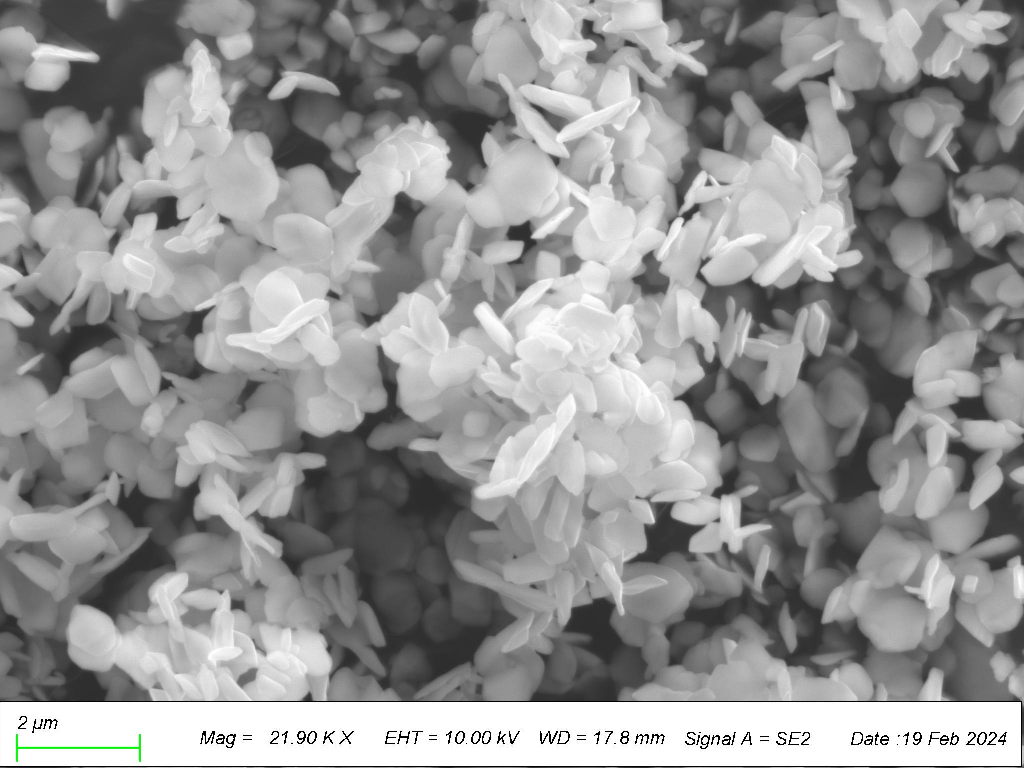
\includegraphics[width=\textwidth]{goe_pig_treatedRed19.pdf}
    \caption{Reacted (red) product}
    \label{fig:gt_pigment_red}
  \end{subfigure}\hfill
  \begin{subfigure}[t]{0.48\textwidth}
    \centering
    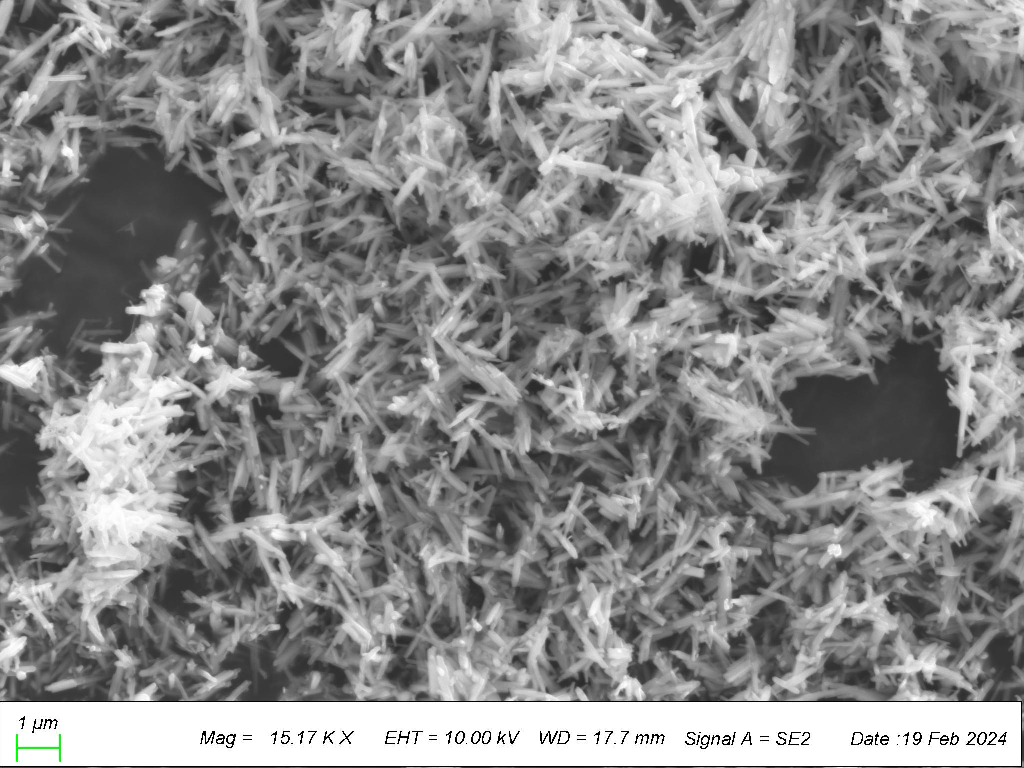
\includegraphics[width=\textwidth]{goe_pig_treatedYellow37.pdf}
    \caption{Unreacted (yellow) pigment}
    \label{fig:gt_pigment_yellow}
  \end{subfigure}
  \caption{Secondary electron images of synthetic goethite pigment after hydrothermal treatment
  at 200--250~$^\circ$C for about a day (\S\ref{sec:gt_pigment_methods}). (a) Material from a
  completely reacted (red) ampoule: the acicular goethite has been replaced by equant to platy
  crystals $\sim$0.5--1~\textmu m across, interpreted as hematite. (b) Material from an
  unreacted (yellow) ampoule, which retains the acicular habit of the starting pigment. The change
  in crystal habit requires dissolution of goethite and precipitation of hematite from the fluid,
  and the all-or-nothing outcome of the experiments indicates that the reaction is limited by
  nucleation and proceeds rapidly once it begins.}
  \label{fig:gt_pigment}
\end{figure}

The distribution of outcomes is itself diagnostic. Conversion either went to completion within
a fluid-connected volume or did not occur at all, even where reacted and unreacted pigment shared
the same ampoule and thermal history. This is the behavior of a nucleation-limited process:
once hematite nucleates, the reaction proceeds rapidly to completion, and where it does not
nucleate, goethite persists for the full run. The fluid-mediated pathway is therefore governed,
like the solid-state pathway, by the difficulty of forming a hematite nucleus rather than by the
rate at which hematite grows.

We conclude that water-saturated conditions do not by themselves exclude fluid-mediated
conversion of goethite, even where solid-state conversion is suppressed (\S\ref{sec:gt_nucleation}). Whether that pathway operates
depends on the solution chemistry. For the natural sample in distilled water,
\S\ref{sec:gt_hydro} shows that the release is diffusive; a nucleation-limited, all-or-nothing
reaction would also be expected to release helium abruptly rather than in the smooth,
history-dependent manner observed. For samples whose chemistry is less well characterized, the
absence of conversion should be verified directly, for example by post-run X-ray diffraction or
electron microscopy.

\paragraph{\texorpdfstring{High Helium Retentivity of
Win-06-01b-HT}{ High Helium Retentivity of Win-06-01b-HT}}\label{high-helium-retentivity-of-win-06-01b-ht}

Apparent diffusivities calculated from helium step heats on the
hydrothermal experiment on Win-06-01b goethite are clearly resolved and
much lower than the apparent diffusivities calculated for the same
sample in vacuum by \citet{monteiro2017} and \citet{farley2024} for all steps
after the first few (Fig.~\ref{fig:gt_arrhenius}b, Fig.~\ref{fig:ch2-arrhenius-zoom}, Fig.~\ref{fig:ch2-delta-zoom}). Diffusivities calculated
from the hydrothermal experiment are approximately seven natural log
units lower than the earlier experiments in vacuum on the same sample. This high
helium retentivity is explored through three lenses: closure temperature
of cooling samples \citep{dodson1973}, isothermal diffusion \citep{wolf1998}, and through comparison with step heats of other polycrystalline
samples. Strictly speaking, both closure temperatures and retention
estimations under isothermal diffusion only apply to helium loss
occurring exclusively via thermally activated volume diffusion with
known domain size. While the results presented here on a polycrystalline
sample are consistent with a thermally activated volume diffusive
process for helium loss in goethite under hydrothermal conditions, they
do not exclude other processes (such as goethite
dehydration/decomposition/recrystallization) or potential complexities
related to radiation damage and crystal defects on bulk diffusion
\citep{bassal2022}, nor do they permit estimation of the diffusivity
at infinite temperature (D0).

If the slope and intercept on the regression of 3He apparent
diffusivities from this experiment are taken to represent a real
diffusion domain for goethite, then a closure temperature can be
calculated for this domain. Considering uncertainty only in the
intercept (D\textsubscript{0}/a\textsuperscript{2}) term and a cooling rate of 10°C/Ma, the closure
temperature for that domain would be \ChTwoTc ± \ChTwoTcErr °C.

Goethite is formed near Earth's surface and thus U-Th/He geochronology
is most typically applied to date surface processes \citep{heim2006,yappshuster2011,vasconcelos2013,danisik2013,monteiro2014,hofmann2017,allard2018}. For
crystals of goethite grown near the surface that are found near the
surface, the concept of a closure temperature is poorly applicable, as
it necessarily assumes a cooling rate \citep{dodson1973}. In such cases, a
better measure of retentivity is an analysis of isothermal retentivity
over time \citep{wolf1998}, which is commonly expressed in terms of
t'/t, where t' is the helium age and t is the isothermal holding time
(most often the `real age'). For an isothermal holding time of 100 Ma at
40°C, a diffusive domain with the parameters obtained from the
regression of 3He apparent diffusivities of Win-06-01b-HT has a t'/t = 0.968, where t'/t = 1 corresponds to perfect retentivity. Fig.~\ref{fig:ch2-isothermal-retention}
shows isothermal holding time against helium age for this same domain
for 4 different temperatures. At 25°C, this domain is nearly
quantitatively retentive of helium even at billion-year time scales. The
results presented here qualitatively support that goethite is highly
retentive of helium at surface conditions, even at 100-million-year
timescales.
\begin{figure}[htbp]
\centering
\includegraphics[width=0.8\textwidth]{PRP_goethite_winsor.pdf}
\caption{Isothermal retention plot \citep{wolf1998} for helium in goethite corresponding to the ``Stage 1'' reference line regression on the hydrothermal experiment. Helium hosted in a diffusion domain with these diffusion parameters would be nearly perfectly retentive at billion-year timescales at 25\textdegree C. At 40\textdegree C, the equilibrium age for this domain (the helium age at which radiogenic helium production and diffusive loss are equal) is 33.2 billion years, attained after 50.4 billion years.}
\label{fig:ch2-isothermal-retention}
\end{figure}

It is difficult to use Arrhenius plots to compare many samples' helium
retentivities. \citet{farley2024} report that linear regressions on
apparent diffusivities calculated from helium step heat data on goethite
in vacuum can be fit to yield widely variable diffusive parameters even
for a single sample (e.g. activation energies ranging from 107 to 176
kJ/mol within a single experiment on YAN-0201 AC). Similarly,
regressions on helium step heat data of polycrystalline materials can
yield erroneous activation energies when not applied carefully \citep{farley2018}. Because of the complexity of comparing Arrhenius plots of
calculated apparent diffusivities for polycrystalline samples with
differing heating schedules, it is advantageous to convert heating
schedules to some parameter that can be compared easily between
experiments. One effective way to reduce the complexity of step heat
experiments to visualize helium retentivity is to ``flatten'' a thermal
history to a dimensionless diffusive timescale: the Fourier number (Fo =
Dt/a\textsuperscript{2}). This approach offers similar benefits to Delta plots
\citep{farley2018} or r/r0 plots \citep{lovera1991}, but is optimized to
qualitatively compare the helium retentivities of polycrystalline
samples for a given thermal history (expressed as diffusive time).

For a given diffusive domain, a Fourier number of Fo $\approx$ 1 corresponds to
the complete degassing of that domain. Complex heating schedules can be
converted to Fourier numbers by assuming a reference line similarly to a
Delta or r/r0 plot \citep{lovera1991,farley2018}. This procedure
is especially useful for MDD (Multiple Diffusion Domain) systems, where
the apparent diffusivities decrease over the course of a step heat
experiment as the least retentive domains are degassed. For a single
spherical diffusion domain, the fraction of helium released is a
function of the Fourier number alone \citep{crank1979,fechtigkalbitzer1966}. If the activation energy of the reference
Fourier number is the same as the activation energy of diffusion, then
the amount of helium released in that domain then is an exact function
of the reference Fourier number multiplied by a constant. Thus, a plot
with reference Fourier numbers against cumulative fractional helium
yields for different samples will yield the same geometries and
interrelationships regardless of the intercept used to calculate the
reference Fourier numbers; the values of the reference Fourier numbers
will be arbitrary and only meaningful as relative diffusive time.
Another implication is that different aliquots of the same sample should
appear identical in this space regardless of heating schedule (see the vacuum step heats of
Win-06-01b and the overlapping hematite samples in Fig.~\ref{fig:ch2-fourier-hematite-ref}).
Many such plots were generated with a variety of activation energies between
149 kJ/mol to 171 kJ/mol, but the relative positions of the degassing curves for all samples are preserved, 
illustrating the utility of this approach even for comparing helium retentivity between different minerals. 

Fig.~\ref{fig:ch2-fourier-hematite-ref} compares the step heat results of Win-06-01b-HT with 11
step heat experiments of 3 samples of polycrystalline hematite and 9
step heat experiments of 2 samples of goethite in Vacuum, including
Win-06-01b. In a thermal-history normalized space, it is obvious that
goethite in vacuum and hematite define well-separated populations and
goethite in vacuum is far less retentive of helium than hematite. Most
interestingly, the most retentive sample on these plots is clearly the
Win-06-01b-HT goethite under water-saturated conditions, at least for the
14.7\% of the total 3He hosted in the least retentive domains. This plot shows
that step heat results for different, unrelated goethite samples in vacuum are more similar to one
another than step heat results of the same sample at different water
activities.
\begin{figure}[htbp]
\centering
\includegraphics[width=0.75\textwidth]{Fo_Plot_hematite_ref_HematiteGoethite.pdf}
\caption{Heating schedules for polycrystalline goethite and hematite samples are flattened to reference Fourier numbers, dimensionless numbers that can be thought of as integrated thermal history, allowing for easy comparison of entire helium step heat experiments. The 3He cumulative fractional yield is plotted on the $y$ axis as a function of Fourier number in log scale on the $x$ axis. Curves on the left of the plot degas earlier within a given thermal history than the curves on the right. Hematite and goethite step heats in vacuum each cluster closely together, forming distinct populations. Most strikingly, the hydrothermal Win-06-01b-HT experiment is the most helium-retentive polycrystalline sample on the plot, at least until the experiment's end at a cumulative fractional yield $\sim$15\% F3He. In vacuum, all hematite samples are significantly more retentive of helium than all goethite samples, with some limited exceptions for the least retentive domains holding $<$5\% of the total helium. Win-06-01b step heat experiments in vacuum are indistinguishable from the Capao samples in vacuum (the two leftmost goethites are Capao samples; the rest of the Capao samples closely cluster with Win-06-01b in vacuum). The differences in the curves here reflect differences in grain size distributions for hematite, and some combination of grain size and dehydration rate (due to variable water pressure in the experimental vessel and crystal aggregate size) for goethite. Vacuum step heats of 11 aliquots of 4 samples of polycrystalline hematite from the Grand Canyon, Arizona \citep{farleyflowers2012} and the Gogebic Range, Michigan \citep{farleymckeon2015}, and 9 aliquots of Win-06-01b and Capao goethite from Minas Gerais, Brazil \citep{monteiro2017,farley2024} are plotted here. The reference $D/a^2$ values are calculated for 1\textmu m domains of hematite (ln($D_0$) = 0.66; $E_a$ = 171 kJ/mol: \citep{farley2018}), and the reference curve for the degassing of 1\textmu m spherical domains of hematite with uniformly distributed 3He is calculated using the forward equations of \citet{fechtigkalbitzer1966}.}
\label{fig:ch2-fourier-hematite-ref}
\end{figure}

\paragraph{Profiling Radiogenic Helium Loss with $\frac{^4He}{^3He}$ Ratios of Win-06-01b-HT}\label{spectra-of-win-06-01b-ht}

Bulk-normalized 4He/3He ratios in step heats of irradiated samples
measure rounding concentration profiles by natural helium loss, if the
loss mechanism in nature and in the laboratory share the same geometry
\citep{shuster2004,farley2024}. Aside from the first
experimental step, bulk-normalized 4/3 ratios for all experiments begin
at vanishingly small values and steeply increase at first, with the rate
of increase slowing as the experiments proceed (Fig.~\ref{fig:ch2-ratio-spectra}). This
behavior is consistent with complete then partial loss of radiogenic
helium in nature in the least retentive domains and is observed in all
step heat experiments on irradiated goethite \citep{farley2024}. The
hydrothermal experiment, however, records lower bulk-normalized 4/3
ratios than the vacuum experiments at any given $\Sigma F_{3\mathrm{He}}$ for the duration
of the experiment. Similarly, the approach to the 4/3 plateau varies
between the three experiments: a high bulk normalized 4/3 He plateau is
most decisively represented in the \citet{farley2024} experiment,
whereas the 4/3 ratios in the step heats of \citet{monteiro2017} transition
more gradually before reaching a plateau later in the experiment, while
the increase in 4/3 ratios is slowest for the hydrothermal experiment
(Fig.~\ref{fig:ch2-ratio-spectra}). This suggests that the geometry of helium loss
differs between the hydrothermal and vacuum experiments, and could be explained by the relative
dominance of dehydration processes or their mode of spatial propagation as a
function of water pressure, where the smoothest 4/3 spectra are
generated by higher water pressures. We interpret this experimental control on the
4He/3He spectra to be the relative importance of goethite dehydration and helium
diffusion through crystalline goethite in governing the geometry of helium loss from
the sample. This interpretation is consistent with the kinetic analysis of
\S\ref{sec:gt_vacuum}--\ref{sec:gt_hydro}: in vacuum, grains release their integrated
inventory as they convert to hematite, whereas under hydrothermal conditions the release is
diffusive. If the geometry of helium loss due to dehydration and due to diffusion
differ, then the 4He/3He spectra of goethite measured in vacuum may not
straightforwardly encode the geometry or history of helium loss in the way that such
data faithfully encode this history in phases such as hematite or apatite
\citep{farleymckeon2015,shuster2004}. This claim rests entirely upon the correctness
of the 4He data reported here, for which each step yield is somewhat small, most often
between 0.15 and 0.5 nccSTP. More 4He/3He spectra of goethite under hydrothermal
conditions, with stronger 4He signals, are needed to investigate this hypothesis
further. The experiment in \citet{farley2024} was open to a liquid nitrogen trap during heating, which would
maintain lower water pressures than \citet{monteiro2017}, who in turn held
Win-06-01b at much lower water pressures than the hydrothermal
experiment presented in this work. While the hydrothermal experiment did
not reach a plateau, it may have if the experiment was allowed to
proceed further.

Interestingly, both vacuum experiments show a maximum bulk normalized
4/3 He ratio of \textasciitilde{} 1.1 at or before $\Sigma F_{3\mathrm{He}}$ = 0.88, after
which the bulk normalized 4/3 He decreases to \textasciitilde0.9,
suggesting that these values are independent of heating schedule and may
reflect a material property of Win-06-01b.

Both vacuum experiments record a somewhat high 4/3 ratio for the first
measurement that is not observed in the hydrothermal experiment (Fig.~\ref{fig:ch2-ratio-spectra}). This feature represents a very small amount of the total helium
and could be related to dehydration of poorly retentive domains in the
vacuum, or it may have been lost in the hydrothermal experiment while
the ampoule was held at 70°C to degas entrained atmosphere before the
initiation of the experiment. This small abundance of poorly retained
4He observed in the vacuum experiments could be related to physisorption
of atmospheric helium \citep{protin2016}. In any case, it represents
a negligible fraction of the 4He contained in Win-06-01b.
\begin{figure}[htbp]
\centering
\includegraphics[width=0.8\textwidth]{Comparative_Ratios_Dtplot_WinsorGT_VacuumHDMKAF.pdf}
\caption{Bulk-normalized 4/3 ratios for Win-06-01b goethite step heats against cumulative fractional 3He yield. The hydrothermal experiment shows lower bulk-normalized 4/3He ratios at a given $\Sigma F_{3He}$ for the entire duration of the experiment, besides the very first step. All experiments' 4/3He ratios begin at very small values and increase steeply at first, which is consistent with complete then partial loss of radiogenic helium in nature for the least retentive helium domains. The rate of increase slows between $\Sigma F_{3He}$ of 0.05 to 0.2 for all experiments. Each step is drawn as a bar spanning its starting to ending $\Sigma F_{3He}$. The hydrothermal experiment is drawn at the bounding method's central 4/3He ratio for each step, vacuum steps are drawn as lines at their ratios, and thin vertical lines join adjacent steps. For visual continuity, the gap left by excluded hydrothermal steps is bridged by extending the preceding step's ratio across its first half and the following step's ratio across its second half. The horizontal axis changes scale at $\Sigma F_{3He} = 0.2$ (double slash): the left two-thirds of the plot shows $\Sigma F_{3He}$ from 0 to 0.2 and the right third shows 0.2 to 1; 10 of 34 hydrothermal analyses are excluded, either because the upper and lower bounds of $\omega$ cannot be computed for the early steps before $\lambda t$ was large enough to assume a steady-state permeation condition, or because the measured 3He signal for that step is below 0.1 pccSTP and too low-signal to give a reliable ratio.}
\label{fig:ch2-ratio-spectra}
\end{figure}

% =============================================================================
% Thermodynamics of goethite dehydroxylation, consolidated at the end of the
% Discussion (moved 2026-09-29): model, stability, and nucleation control.
% =============================================================================
% --- Added 2026-09-25 (goethite stability integration; see CHANGES_JOURNAL.md) ---
% Figures for the goethite stability/kinetics paragraphs below and in the
% Discussion are produced by Chapter2/Figures/fig_goethite_hematite_phase_diagram.py,
% fig_goethite_vacuum_kinetics.py and fig_goethite_hydrothermal_tests.py.
\paragraph{Thermodynamic Model of Goethite Dehydroxylation}\label{sec:gt_thermo_methods}

The preceding sections establish from the release patterns alone that the vacuum step heats of
Win-06-01b record conversion to hematite, whereas the hydrothermal step heat records diffusion
without detectable dehydration. Here we use the thermodynamics of goethite dehydroxylation to
explain why water has this effect (\S\ref{sec:gt_thermo}) and to estimate how much solid-state
conversion could have occurred in the hydrothermal experiment (\S\ref{sec:gt_nucleation}).

Goethite breaks down to hematite by the dehydroxylation reaction
\begin{equation}
  2\,\alpha\text{-FeOOH} \;\rightleftharpoons\; \alpha\text{-Fe}_2\text{O}_3 + \text{H}_2\text{O}_{(\text{fluid})},
  \label{eq:gt_rxn}
\end{equation}
whose Gibbs energy change, written per mole of hematite formed, is
\begin{equation}
  \Delta G_r(T,P) = G_{\mathrm{hem}}(T,P) + G_{\mathrm{w}}(T,P) - 2\,G_{\mathrm{goe}}(T,P) + \Delta G_{\mathrm{surf}} .
  \label{eq:gt_dGr}
\end{equation}
where $\Delta G_r$ is the Gibbs energy change of the reaction and $G_{\mathrm{hem}}$, $G_{\mathrm{w}}$, and $G_{\mathrm{goe}}$ are the Gibbs energies of hematite, water, and goethite, respectively. 
$\Delta G_{\mathrm{surf}}$ is the surface energy contribution, which must to be considered to reproduce observed phase stability \citep{navrotsky2008}. 
Goethite is stable where $\Delta G_r>0$ and hematite plus water where $\Delta G_r<0$. The values and equations used to evaluate each of these terms is given in the supplement: \S\ref{sec:eqm-thermo}.

% --- Added 2026-09-25 (goethite stability integration; see CHANGES_JOURNAL.md) ---
\paragraph{Thermodynamic Stability of Goethite under Experimental Conditions}\label{sec:gt_thermo}

The thermodynamic model of \S\ref{sec:gt_thermo_methods} can be used to calculate the stability field for
goethite with respect to dehydroxylation to hematite and water in $\log P_{\mathrm{H_2O}}$--$T$ space (Fig.~\ref{fig:gt_PT}). This 
phase diagram communicates several important features of the goethite--hematite--water system that are relevant to the experiments considered here:
\begin{enumerate}
  \item Goethite is not stable at the conditions of any of the experiments considered here, in water or in vacuum, in spite of the evidence that it did not react in the water-saturated experiment. Thus, we hypothesize that the reaction is kinetically inhibited for goethite under these conditions.
  \item The stability of goethite is strongly dependent on the partial pressure of water below and up to water saturation. Above the saturation pressure, water is liquid and contributes far less to the reaction volume than it does as a gas. The reaction volume $\Delta V_r = V_{\mathrm{hem}} + V_{\mathrm{w}} - 2V_{\mathrm{goe}} \approx +6.6$~cm$^3$ is small,and the boundary becomes nearly vertical in $\log P_{\mathrm{H_2O}}$--$T$ space.
  \item The stability of goethite is strongly dependent on grain size, with smaller grains being more stable than larger grains. At water saturation, bulk goethite is stable below 18~$^\circ$C, 100~nm goethite below 28~$^\circ$C, and 10~nm goethite below 108~$^\circ$C. 
\end{enumerate}

\begin{figure}[htbp]
  \centering
  \includegraphics[width=0.7\linewidth]{goethite_hematite_Ph2o_T_hydrated.pdf}
  \caption{Goethite--hematite--water equilibrium in $\log P_{\mathrm{H_2O}}$--$T$ space for bulk
  goethite and for 100 and 10~nm grains with hydrated surfaces, compared at equal surface area
  per mole of Fe (Eq.~\eqref{eq:gt_equalarea}). Goethite is stable above and to the left of each
  curve. The dash-dot curves illustrate the absolute uncertainty: the bulk boundary is shifted by the $\pm1.4$~kJ\,mol$^{-1}$ FeOOH uncertainty of
  \citet{majzlan2003}. The blue dotted curve shows the water vapor saturation pressure; liquid water is present at and above this curve. The thermodynamic data used to compute the phase diagram are in
  Table~\ref{tab:gt_thermo_data}.}
  \label{fig:gt_PT}
\end{figure}

Stability alone does not determine what happens in a step heat; the rate of conversion controls
whether this equilibrium state is reached or if the reaction proceeds at all,
and that depends on the chemical potential of the reaction: $\Delta\mu$. Table~\ref{tab:gt_dmu} gives the bulk driving
forces at the experimental temperatures, evaluated with IAPWS-95 water. At saturation,
$\Delta\mu$ is 6--11~kJ, only 1.6--2.4 times $RT$. Under the vacuum of a step-heating line
($P_{\mathrm{H_2O}}\approx10^{-8}$~atm) it is 76--106~kJ, about ten times larger. The chemical
potential of water is therefore the key variable separating the two experimental settings.

\begin{table}[htbp]
  \centering
  \caption{Bulk driving force for hematite formation, $\Delta\mu = -\Delta G_r$ (kJ per mole Fe$_2$O$_3$), at water saturation and at $P_{\mathrm{H_2O}} = 10^{-8}$~atm.}
  \label{tab:gt_dmu}
  \begin{tabular}{cccccc}
    \hline
    $T$ ($^\circ$C) & $P_{\mathrm{sat}}$ (bar) & $\Delta\mu_{\mathrm{sat}}$ & $\Delta\mu_{\mathrm{sat}}/RT$ & $\Delta\mu_{\mathrm{vac}}$ & $(\Delta\mu_{\mathrm{vac}}/\Delta\mu_{\mathrm{sat}})^2$ \\
    \hline
    150 & 4.76  & 5.68  & 1.61 & 75.8  & 178 \\
    175 & 8.93  & 6.88  & 1.84 & 83.4  & 147 \\
    200 & 15.55 & 8.10  & 2.06 & 91.0  & 126 \\
    225 & 25.50 & 9.36  & 2.26 & 98.5  & 111 \\
    250 & 39.76 & 10.65 & 2.45 & 106.0 & 99  \\
    \hline
  \end{tabular}
\end{table}

\paragraph{Water Suppresses Solid-State Conversion of Goethite}\label{sec:gt_nucleation}

\textit{What the data require.} The hydrothermal observations themselves bound how fast
goethite could have converted to hematite in water. Under the vacuum kinetics of
Eq.~\eqref{eq:gt_line}, the hydrothermal schedule gives
$\sum_i k_{\mathrm{vac}}(T_i)\,\Delta t_i \approx \ChTwoKinSumKdt$, enough to convert the sample
completely many times over. Suppose instead that water lowers the conversion rate by a factor
$R = k_{\mathrm{sat}}/k_{\mathrm{vac}}$. Even if every atom of the observed $^3$He release came from
conversion, the conversion would be only $\alpha = F/(1-\phi) = \ChTwoKinHTFEnd/\ChTwoKinOneMinusPhi =
\ChTwoKinHTAlphaObs$, which requires $R \le 10^{\ChTwoKinLogRObs}$. The release is instead diffusive
(\S\ref{sec:gt_hydro}), and keeping conversion below 1\% requires $R \le 10^{\ChTwoKinLogRDetect}$.
Without any assumption about mechanism, then, water must slow solid-state conversion by more
than two orders of magnitude, and plausibly by nearly four. The question for the rest of this
section is whether a physically reasonable rate law, calibrated on the vacuum data alone,
predicts suppression of this size.

\textit{Candidate rate laws.} The only direct information on how water affects the conversion rate
comes from the two KAF steps with the trap isolated, where the rate fell by a factor
$s$ (\S\ref{sec:gt_vacuum}) as $P_{\mathrm{H_2O}}$ rose from $\sim10^{-3}$~Pa to a few Pa. Each
temperature therefore supplies one calibration pair ($s$, $P_{\mathrm{off}}$), and predicting the
hydrothermal experiment means extrapolating about six orders of magnitude in $P_{\mathrm{H_2O}}$, to
water saturation. The result is set by the assumed functional form. Water vapor is well known to
retard dehydration and dehydroxylation reactions, through the reverse reaction, adsorption on the
reaction interface, or both \citep{topley1935,lvov2007,koga2019}. We compare three laws,
each calibrated on the same trap-isolated steps (Table~\ref{tab:gt_ratelaws}):
\begin{enumerate}
  \item \textit{Nucleation control} (classical nucleation theory, developed below), in which
  $\ln k$ falls as $-1/\Delta\mu^{2}$, so that the tenfold drop in $\Delta\mu$ between vacuum and
  saturation (Table~\ref{tab:gt_dmu}) raises the barrier a hundredfold.
  \item \textit{Site blocking}, in which adsorbed water occupies reactive sites,
  $k\propto 1/(1+KP_{\mathrm{H_2O}})$ (Langmuir), with $K$ calibrated at the trap-isolated steps
  and held constant.
  \item \textit{A power law}, $k\propto P_{\mathrm{H_2O}}^{-n}$, a deliberately weak dependence.
\end{enumerate}
A fourth possibility, a rate linear in the driving force, $k\propto1-\exp(-\Delta\mu/RT)$, has no free
parameter and cannot reproduce the calibration: it predicts $s=\ChTwoKinLinearS$ at the trap-isolated
steps, against the observed \ChTwoKinTrapSuppLow{} and \ChTwoKinTrapSuppHigh.

\begin{table}[htbp]
  \centering
  \caption{Water-inhibition rate laws calibrated on the two trap-isolated KAF steps and applied to
  the hydrothermal schedule. Calibration grid: both steps, $V_{\mathrm{app}} = 190$ and 600~mL, and
  end-of-step or half pressure (Table~\ref{tab:gt_gamma}). Monte Carlo: \ChTwoKinNMC{} draws of the
  step, $s$ (\ChTwoKinSLowRange{} at 230~$^\circ$C and \ChTwoKinSHighRange{} at 240~$^\circ$C across
  first-order and contracting-sphere reductions and choice of neighboring steps), $V_{\mathrm{app}}$,
  the time-averaged pressure and, for nucleation control, a common $\pm2.8$~kJ offset in
  $\Delta G_r$; 95\% range. Units: $\gamma_{\mathrm{eff}}$ in J\,m$^{-2}$, $K$ in Pa$^{-1}$. The data require $\alpha\le\ChTwoKinHTAlphaObs$ and, given the diffusive
  release, $\alpha<0.01$ (\S\ref{sec:gt_supp_ratelaws}).}
  \label{tab:gt_ratelaws}
  \begin{footnotesize}
  \setlength{\tabcolsep}{4pt}
  \begin{tabular}{lcccc}
    \hline
    Law & Parameter & $\log_{10}\dfrac{k_{\mathrm{sat}}}{k_{\mathrm{vac}}}$, 250~$^\circ$C
      & $\alpha$, grid & $\alpha$, Monte Carlo \\
    \hline
    Nucleation
      & $\gamma_{\mathrm{eff}}$ = \ChTwoKinGammaLo--\ChTwoKinGammaHi
      & $\ChTwoKinCNTLogRLo$ to $\ChTwoKinCNTLogRHi$
      & $10^{\ChTwoKinCNTLogAlphaLo}$--$10^{\ChTwoKinCNTLogAlphaHi}$
      & $10^{\ChTwoKinMCCNTLo}$--$10^{\ChTwoKinMCCNTHi}$ \\
    Site blocking
      & $K$ = \ChTwoKinLangKLo--\ChTwoKinLangKHi
      & $\ChTwoKinLangLogRLo$ to $\ChTwoKinLangLogRHi$
      & $10^{\ChTwoKinLangLogAlphaLo}$--$10^{\ChTwoKinLangLogAlphaHi}$
      & $10^{\ChTwoKinMCLangLo}$--$10^{\ChTwoKinMCLangHi}$ \\
    Power law
      & $n$ = \ChTwoKinPowNLo--\ChTwoKinPowNHi
      & $\ChTwoKinPowLogRLo$ to $\ChTwoKinPowLogRHi$
      & \ChTwoKinPowAlphaLo--\ChTwoKinPowAlphaHi
      & \ChTwoKinMCPowAlphaLo--1.00 \\
    \hline
  \end{tabular}
  \end{footnotesize}
\end{table}

All three laws fit the calibration equally well, because each has one free parameter and each
temperature supplies one number. They diverge by fifty orders of magnitude at saturation, but the
hydrothermal data discriminate among them. The power law predicts that the hydrothermal schedule
converted \ChTwoKinPowAlphaLo--\ChTwoKinPowAlphaHi{} of the sample, which would have released most of
the $^3$He abruptly; only \ChTwoKinHTFEnd{} was released, smoothly and with the history and time
dependence of diffusion. Site blocking and nucleation control both predict conversion well below
1\%. The conclusion that solid-state conversion
contributed negligibly to the hydrothermal release therefore holds for every law consistent with
both data sets, but the magnitude of the suppression, $k_{\mathrm{sat}}/k_{\mathrm{vac}}$ from $10^{\ChTwoKinLangLogRHi}$ to
$10^{\ChTwoKinCNTLogRLo}$ at 250~$^\circ$C, is set by the assumed law and is not constrained by the
data. The nucleation
interpretation developed below is one physically motivated explanation of why water is so
effective, not a measurement of the suppression.

\textit{Nucleation barrier.} In classical nucleation theory \citep{gibbs1878,volmer1926,becker1935},
reviewed by \citet{christian2002}, \citet{kashchiev2000} and, for mineral systems,
\citet{deyoreo2003} and \citet{lasaga1998}, a spherical hematite nucleus of radius $r$ has free
energy
\begin{equation}
  \Delta G(r) = -\frac{4}{3}\pi r^{3}\,\frac{\Delta\mu}{V_{\mathrm{hem}}} + 4\pi r^{2}\gamma,
\end{equation}
where $\Delta\mu$ is the driving force per mole of Fe$_2$O$_3$ (Table~\ref{tab:gt_dmu}),
$V_{\mathrm{hem}}$ the molar volume and $\gamma$ the energy of the interface surrounding the
nucleus. The first term is the free energy released by transforming the nucleus volume. The second
is the cost of creating its interface. Setting $d\Delta G/dr=0$ gives the critical radius
$r^{*} = 2\gamma V_{\mathrm{hem}}/\Delta\mu$ (nuclei larger than this are stable and will grow) and the barrier height
\begin{equation}
  \Delta G^{*} = \frac{16\pi\,\gamma^{3}\,V_{\mathrm{hem}}^{2}}{3\,\Delta\mu^{2}} .
  \label{eq:gt_barrier}
\end{equation}
Written per formula unit, $V_{\mathrm{hem}}\to V_{\mathrm{hem}}/N_A$ and $\Delta\mu\to\Delta\mu/N_A$, so
Avogadro's number cancels and Eq.~\eqref{eq:gt_barrier} is directly the barrier per nucleus in
joules. In the first-order limit of \S\ref{sec:gt_vacuum}, the rate constant is a nucleation
rate of the form derived by \citet{turnbull1949},
\begin{gather}
  k = A\exp\!\left(-\frac{E_a}{RT}\right)\exp\!\left(-\frac{\Delta G^{*}}{k_B T}\right), \notag\\
  \frac{\Delta G^{*}}{k_B T} = \frac{C\gamma^{3}}{T\,\Delta\mu^{2}},
  \qquad
  C \equiv \frac{16\pi V_{\mathrm{hem}}^{2}}{3k_B} = 1.112\times10^{15}~\mathrm{m^6\,K\,J^{-1}\,mol^{-2}} ,
  \label{eq:gt_knuc}
\end{gather}
where $A\exp(-E_a/RT)$ describes the atomic mobility and $\exp(-\Delta G^{*}/k_BT)$ is the
equilibrium fraction of sites occupied by critical nuclei. The barrier scales as $\gamma^3/\Delta\mu^2$. Between vacuum and water
saturation, $\Delta\mu$ falls tenfold and the barrier rises by the factor in the last column of
Table~\ref{tab:gt_dmu}: about 100 at 250~$^\circ$C and nearly 180 at 150~$^\circ$C.

\textit{An upper bound on the vacuum barrier.} The vacuum conversion rate is observed, so the
barrier that controls it cannot exceed what the fastest conceivable prefactor allows. In
transition-state theory \citep{eyring1935} no elementary step is faster than $k_BT/h$, which is
$1.09\times10^{13}$~s$^{-1}$ at 250~$^\circ$C. If every one of the $N$ formula units in a grain were a
nucleation site attempting at this frequency, the per-grain rate could not exceed
$N(k_BT/h)\exp(-\Delta G^{*}/k_BT)$. A 1~\textmu m goethite sphere contains
$N = (\pi d^3/6)/(V_{\mathrm{goe}}/N_A) = 1.5\times10^{10}$ formula units. Requiring this ceiling to
reach the observed $k_{\mathrm{vac}} = \ChTwoKinKTwoFifty$~s$^{-1}$ at 250~$^\circ$C (Eq.~\eqref{eq:gt_line})
gives
\begin{equation}
  \frac{\Delta G^{*}_{\mathrm{vac}}}{k_BT} \le \ln\frac{N\,k_BT/h}{k_{\mathrm{vac}}}
  = \ln\frac{1.5\times10^{10}\times1.09\times10^{13}}{\ChTwoKinKTwoFifty} = \ChTwoKinCeiling .
  \label{eq:gt_ceiling}
\end{equation}
A tenfold larger grain raises the bound by only $\ln 1000 = 7$. Real prefactors are smaller, so the
true barrier is lower still.

\textit{Nucleation must be internal.} The surface energies of \citet{navrotsky2008} fail this
bound by a wide margin. If the nucleus were bounded by a free, anhydrous hematite surface
($\gamma = 1.90$~J\,m$^{-2}$, $\Delta\mu = 106.0$~kJ at 250~$^\circ$C), Eq.~\eqref{eq:gt_knuc} would give
$\Delta G^{*}/k_BT = 1.3\times10^{3}$. Nucleation on a goethite surface lowers this. For a nucleus
shaped as a spherical cap on a flat substrate, the barrier is reduced by the purely geometric
factor
$f(\theta) = (2+\cos\theta)(1-\cos\theta)^2/4 \le 1$, where the contact angle $\theta$ is set by the
balance of interfacial tensions at the triple junction (Young's equation),
$\cos\theta = (\gamma_{\mathrm{goe}} - \gamma_{\mathrm{hem|goe}})/\gamma_{\mathrm{hem}}$
\citep{volmer1926,turnbull1950}. Even with a hematite--goethite interfacial energy of zero,
$\cos\theta \le 0.91/1.90 = 0.48$, $f\ge0.17$ and $\Delta G^{*}/k_BT\ge2.2\times10^{2}$. No
non-negative interfacial energy brings nucleation on free surfaces within the bound of
Eq.~\eqref{eq:gt_ceiling}. Hematite must therefore nucleate internally, where the only new
interface is between hematite and goethite. This agrees with the known mechanism: goethite
dehydroxylates topotactically, the hematite inherits the oxygen framework and orientation of the
parent, and the pseudomorph develops pores and twinned hematite domains
\citep{limadefaria1963,watari1979,watari1983,cudennec2005}. We are not aware of a measured or
calculated energy for the goethite--hematite interface. In what follows, $\gamma$ is replaced by an
effective parameter $\gamma_{\mathrm{eff}}$, calibrated from the data.

\textit{Calibrating $\gamma_{\mathrm{eff}}$ from the trap-isolated steps.} Isolating the trap
raised $P_{\mathrm{H_2O}}$ in the line and lowered $\Delta\mu$, and the isothermal rate fell by a factor
$s$ (\S\ref{sec:gt_vacuum}). With $A$ and $E_a$ unchanged, Eq.~\eqref{eq:gt_knuc} gives
\begin{equation}
  \ln\frac{1}{s} = \frac{C\gamma_{\mathrm{eff}}^{3}}{T}\left(\frac{1}{\Delta\mu_{\mathrm{off}}^{2}} - \frac{1}{\Delta\mu_{\mathrm{on}}^{2}}\right)
  \quad\Longrightarrow\quad
  \gamma_{\mathrm{eff}} = \left[\frac{T\ln(1/s)}{C\left(\Delta\mu_{\mathrm{off}}^{-2} - \Delta\mu_{\mathrm{on}}^{-2}\right)}\right]^{1/3}.
  \label{eq:gt_gamma_cal}
\end{equation}
The driving forces are evaluated as follows.
\begin{enumerate}
  \item $\Delta\mu_{\mathrm{on}}$ and $\Delta\mu_{\mathrm{off}}$ are bulk driving forces,
  $-\Delta G_r$ from Eq.~\eqref{eq:gt_dGr} (\S\ref{sec:eqm-thermo}) with $\Delta G_{\mathrm{surf}} = 0$, at the
  step temperature and with the solids at vacuum.
  \item They differ only through the chemical potential of water: $\Delta\mu_{\mathrm{on}}$ is
  evaluated at $P_{\mathrm{H_2O}} = 10^{-8}$~atm and $\Delta\mu_{\mathrm{off}}$ at the water pressure
  reached with the trap isolated (below). At these pressures (at most 20~Pa), IAPWS-95 and the
  ideal gas agree, and
  $\Delta\mu_{\mathrm{on}} - \Delta\mu_{\mathrm{off}} = RT\ln(P_{\mathrm{off}}/P_{\mathrm{on}})$, which is
  32--41~kJ for the pressures in Table~\ref{tab:gt_gamma}.
  \item Surface terms are omitted in both. The barrier of an internal nucleus depends on the free
  energy per volume of material transformed, not on the external surface of the host grain. The
  grain or domain size of the natural sample is also not characterized. The external surface
  energy of the grain enters the overall thermodynamic stability (\S\ref{sec:gt_thermo}),
  but we do not include it in the barrier. The sensitivity to this choice is small
  (\S\ref{sec:gt_supp_barrier}).
\end{enumerate}
We bound the water pressure with the trap isolated by assuming that all evolved water was in the
vapor, distributed uniformly through an apparatus of volume $V_{\mathrm{app}}$ at 298~K:
\begin{equation}
  P_{\mathrm{H_2O}} = \frac{(m_{\mathrm{w}}/M_{\mathrm{w}})\,RT}{V_{\mathrm{app}}} .
\end{equation}
With $m_{\mathrm{w}} = 0.027$~mg at 230~$^\circ$C and 0.016~mg at 240~$^\circ$C ($1.50$ and
$0.89~\mu$mol), and $190\le V_{\mathrm{app}}\le600$~mL, Table~\ref{tab:gt_gamma} gives the pressures
and the resulting $\gamma_{\mathrm{eff}}$. The pressures are end-of-step values; we also evaluate half
of each as a time average for steady accumulation. This is an upper bound on the pressure, because
some water adsorbs on the walls of the line; a lower true pressure gives a larger
$\gamma_{\mathrm{eff}}$ and more suppression at saturation, so the bound is conservative. Pressure
enters only through $\ln P$ in $\Delta\mu$ and then through a cube root, so a threefold uncertainty
in volume changes $\gamma_{\mathrm{eff}}$ by only about 10\%. The two steps agree within 15\%, and
we adopt $\gamma_{\mathrm{eff}} = 0.16$~J\,m$^{-2}$, with a range of
\ChTwoKinGammaLo--\ChTwoKinGammaHi~J\,m$^{-2}$.

\begin{table}[htbp]
  \centering
  \caption{Water pressure with the trap isolated and the calibrated $\gamma_{\mathrm{eff}}$ (J\,m$^{-2}$; Eq.~\eqref{eq:gt_gamma_cal}).}
  \label{tab:gt_gamma}
  \begin{tabular}{cccccc}
    \hline
    $T$ ($^\circ$C) & $s$ & $V_{\mathrm{app}}$ (mL) & $P_{\mathrm{H_2O}}$ (Pa) & $\gamma_{\mathrm{eff}}$, end-of-step $P$ & $\gamma_{\mathrm{eff}}$, $P/2$ \\
    \hline
    230 & 0.333 & 190 & 19.6 & 0.138 & 0.145 \\
    230 & 0.333 & 600 & 6.2  & 0.150 & 0.158 \\
    240 & 0.224 & 190 & 11.6 & 0.164 & 0.172 \\
    240 & 0.224 & 600 & 3.7  & 0.178 & 0.188 \\
    \hline
  \end{tabular}
\end{table}

\textit{Where classical nucleation theory applies.} The calibration sits outside the range in
which classical nucleation theory has a physical meaning. At 250~$^\circ$C and
$\gamma_{\mathrm{eff}} = \ChTwoKinGammaLo$--$\ChTwoKinGammaHi$~J\,m$^{-2}$, the critical radius under vacuum
is $r^{*} = \ChTwoKinRstarVac$~nm, a nucleus of \ChTwoKinNfuVac{} formula units, and the barrier is
\ChTwoKinBarVac~$k_BT$. Conversion in vacuum is effectively barrierless, consistent with the simple
first-order Arrhenius behavior of both vacuum experiments, and the trap-isolated steps change the
barrier by only about one $k_BT$. At saturation $r^{*} = \ChTwoKinRstarSat$~nm (\ChTwoKinNfuSat{}
formula units) and the barrier is \ChTwoKinBarSat~$k_BT$, a size at which the theory is at best
approximate. The calibration therefore does not measure an interface energy. It fixes the one
free parameter, $B = C\gamma_{\mathrm{eff}}^{3}$, of a rate law in which $\ln k$ falls as
$-B/(T\Delta\mu^{2})$, and $\gamma_{\mathrm{eff}}$ should be read as a phenomenological parameter of the
sample. Its magnitude is similar to the 0.24~J\,m$^{-2}$ calculated for the twin boundaries between
hematite domains formed by dehydrating goethite \citep{saito2016}, but at these length scales the
agreement should not be over-interpreted.

\textit{Translation to water saturation.} For the same sample, with the same $\gamma_{\mathrm{eff}}$
and the same mobility term, only $\Delta\mu$ changes between vacuum and saturation:
\begin{equation}
  \frac{k_{\mathrm{sat}}}{k_{\mathrm{vac}}} = \exp\!\left[-\frac{C\gamma_{\mathrm{eff}}^{3}}{T}\left(\frac{1}{\Delta\mu_{\mathrm{sat}}^{2}} - \frac{1}{\Delta\mu_{\mathrm{vac}}^{2}}\right)\right],
  \label{eq:gt_translate}
\end{equation}
with both driving forces evaluated as in the calibration (bulk, IAPWS-95 water at $P_{\mathrm{sat}}$ and
at $10^{-8}$~atm). For $\gamma_{\mathrm{eff}} = 0.14$, 0.16 and 0.19~J\,m$^{-2}$, this ratio is
$7\times10^{-23}$, $9\times10^{-34}$ and $5\times10^{-56}$ at 250~$^\circ$C, and $5\times10^{-43}$,
$7\times10^{-64}$ and $2\times10^{-106}$ at 200~$^\circ$C.

How large a barrier would still allow detectable conversion follows from the same kinetics. Over
the 442.8~h ($1.59\times10^{6}$~s) hydrothermal experiment, converting even 1\% of the sample
requires $\sum_i k_{\mathrm{sat}}(T_i)\Delta t_i\gtrsim0.01$, i.e., for a barrier that is the same at
every step,
\begin{equation}
  \frac{\Delta G^{*}_{\mathrm{sat}}}{k_BT} \lesssim \ln\frac{\sum_i k_{\mathrm{vac}}(T_i)\,\Delta t_i}{0.01}
  = \ln\frac{\ChTwoKinSumKdt}{0.01} \approx \ChTwoKinDetect ,
\end{equation}
far below the calibrated \ChTwoKinBarSat~$k_BT$. Applying Eq.~\eqref{eq:gt_translate} step by step to the
hydrothermal schedule, with $k_{\mathrm{vac}}$ from Eq.~\eqref{eq:gt_line}, the predicted conversion is
\begin{equation}
  \alpha \approx \sum_i k_{\mathrm{vac}}(T_i)\,\frac{k_{\mathrm{sat}}}{k_{\mathrm{vac}}}(T_i)\,\Delta t_i
  = 10^{\ChTwoKinLogAlphaLow},\ 10^{\ChTwoKinLogAlphaMid},\ 10^{\ChTwoKinLogAlphaHigh}
\end{equation}
for the three values of $\gamma_{\mathrm{eff}}$. Propagating the uncertainties in $s$, the apparatus
volume, the time-averaged pressure and the $\pm2.8$~kJ uncertainty in $\Delta G_r$ gives
$10^{\ChTwoKinMCCNTLo}$ to $10^{\ChTwoKinMCCNTHi}$ (95\%; Table~\ref{tab:gt_ratelaws},
\S\ref{sec:gt_supp_ratelaws}). The thermodynamic offset moves every driving force together; it
barely changes $\gamma_{\mathrm{eff}}$ but contributes most of this spread, because it enters the small
$\Delta\mu_{\mathrm{sat}}$ squared. Even the most permissive calibration,
$\gamma_{\mathrm{eff}} = 0.084$~J\,m$^{-2}$, gives $\alpha = \ChTwoKinAlphaPermissive$. That value would require
0.1~bar of water in the line, far above the volume constraint.

\textit{Assumptions.} This treatment is a consistent physical explanation of the data, not a
proof. It rests on four assumptions.
(i) The slowdown during the trap-isolated steps acts through $\Delta\mu$. If adsorbed water instead
slowed dehydroxylation by blocking reactive sites, the site-blocking law of
Table~\ref{tab:gt_ratelaws} applies; it predicts far less suppression but still no detectable
conversion.
(ii) $\gamma_{\mathrm{eff}}$, $A$ and $E_a$ are the same in vacuum and in water. The
mechanism is internal nucleation in both settings, so only the chemical potential of water
changes.
(iii) The barrier depends on the bulk driving force. Including the surface terms of
Eq.~\eqref{eq:gt_equalarea} for grain sizes down to 10~nm raises the predicted hydrothermal
conversion by about eight orders of magnitude, to $\alpha\approx10^{-23}$
(\S\ref{sec:gt_supp_barrier}).
(iv) Only solid-state conversion is modeled. Conversion by dissolution of goethite and
precipitation of hematite from the fluid is not described by Eq.~\eqref{eq:gt_translate}
(\S\ref{sec:gt_pigment}).
The comparison is valid only between experimental conditions on the same sample. The calibrated
$\gamma_{\mathrm{eff}}$ absorbs the sample's microstructure and should not be transferred to other
goethites.

Assumption (iv) matters for the synthetic pigment of \S\ref{sec:gt_pigment}. Grain size and bulk
thermodynamics do not explain why the pigment blades reacted when the natural goethite did not. At 1~\textmu m, the surface contribution to $\Delta G_r$ is only
$\sim$0.04~kJ, and the bulk driving force at saturation is the same 6--11~kJ for both materials
(Table~\ref{tab:gt_dmu}). The most likely difference is the fluid itself. Commercial iron-oxide
pigments are commonly produced by precipitation from iron-salt solutions. They can carry
residual soluble salts, such as sulfate, and may be surface-treated. Such contaminants would
change the pH and ionic strength of the water they are heated in, and with them the solubility
of Fe(III). The dissolution--precipitation pathway is limited by how much iron the fluid can
carry, so a modest increase in Fe(III) solubility could turn a negligible reaction into a
visible one. Differences in residue loading or in the handling of individual ampoules would also
explain why the outcome was not reproducible. The natural goethite, by contrast, was heated in
distilled water, where near-neutral Fe(III) solubility is very low.
% TODO: check the pigment product data sheet (grade, surface treatment, soluble-salt content, aqueous pH).

\clearpage

\section{Conclusions}\label{conclusions}

Predicting the degree of helium retention and loss to guide
interpretation of U-Th/He dates of natural goethite based on factors
such as grain size, crystallinity, radiation damage, defect density,
impurities, and aluminum substitution remains challenging. Previous
efforts to understand helium loss in natural goethite with step heating
experiments in vacuum have instead queried the kinetics of dehydration
\citep{farley2024}. It remains unclear how informative existing
vacuum helium step heat data are with respect to helium retention and
loss in natural samples. Because goethite dehydration is slowed or
stopped at high water pressure, helium step heats under hydrothermal
conditions are more likely to interrogate the processes controlling
radiogenic helium loss in natural goethite. Hydrothermally treated goethite does not develop the
visible dehydration-induced contraction cracks that goethite heated in vacuum does. The method
presented in this
study leverages the high helium permeability of silica glass to easily
conduct helium step heat experiments under hydrothermal conditions,
achieving internal water pressures up to 86 bars at 300°C using standard
ultra-high vacuum experimental setups \citep{farley1999}.

The experiment conducted on irradiated Win-06-01b represents the first
hydrothermal helium step heat experiment for goethite. Vacuum step heats of the same sample follow
first-order conversion to hematite, whereas the hydrothermal release shows the history and time
dependence of diffusion. The hydrothermal experiment gives apparent
diffusivities approximately seven natural log units below those obtained
from the same sample in vacuum. The corrected 3He array is linear between
7--15\% cumulative yield, with an activation energy of \ChTwoEa ±
\ChTwoEaErr kJ/mol, and its delta plot follows multiple diffusion domain
systematics. Extrapolated to surface conditions, a domain with these
parameters is essentially quantitatively retentive of helium at
billion-year timescales at 25°C. The 4He data require that this domain
experienced helium loss in nature.

The 4He/3He spectrum observed for this sample is distinct from that of the
same sample in vacuum, suggesting that the geometry of helium loss induced
by goethite dehydration is distinct from that of diffusion. More
hydrothermal step heat experiments of goethite are necessary to confirm
this hypothesis.

A thermodynamic and kinetic analysis of goethite dehydroxylation explains why water has this
effect. The hydrothermal release itself requires solid-state conversion to be at least
$10^{2.5}$ times slower in water than in vacuum. Every water-inhibition law consistent with the
vacuum and hydrothermal data predicts negligible conversion at water saturation: by about five
orders of magnitude if water blocks reactive sites, and by tens of orders of magnitude if the
roughly tenfold smaller driving force at saturation raises the barrier to hematite nucleation.
The size of the suppression depends on the rate law, which the present data cannot determine. Fluid-mediated
conversion, which transformed synthetic goethite pigment in qualitative
experiments, and recrystallization cannot be excluded on these grounds alone.
If either contributed, the diffusivities reported here would be upper
bounds and the retentivity a lower bound. Distinguishing these
possibilities, and separating the effects of crystallite size, chemical
composition, and radiation damage, will require further hydrothermal
experiments on irradiated single-crystal goethite of controlled size. The
method described here makes such experiments straightforward.


% =============================================================
%  Chapter 2 Supplementary Information (dissertation-chapter version)
%
%  This is the dissertation-formatted version of
%  Chapter2/Writing/chapter2goethite_SI.tex (the standalone draft).
%  Both wrappers \input{} the SAME shared content file --
%  chapter2goethite_SI_body.tex -- so the science is written and
%  edited in exactly one place. Edit that file, not this one or
%  chapter2goethite_SI.tex, to change text/equations/figures/citations.
%
%  Citations use \citep/\citet against the master references.bib, same
%  as chapter2.tex -- resolved by the single \printbibliography at the
%  end of dissertation.tex, so no local bibliography is needed here.
%
%  Placement: appended at the end of Chapter 2, same convention as
%  Chapter1/chapter1_SI.tex.
%
%  Gets its own title/divider page (\SItitlepage) and its own
%  "2.Ns"-style section numbering (the `ChapterSI` environment), both
%  defined in dissertation_preamble.tex -- see the comment there for the
%  full rationale (this is the Chapter 1 pattern repeated here per the
%  user's request to propagate it to Chapter 2 and beyond).
%
%  NOTE: Do NOT include \documentclass or \begin{document} here.
%        This file is \input{} into dissertation.tex.
% =============================================================

\SItitlepage{Helium Step Heats on Goethite in Water Saturated Conditions Show Diffusive Helium Loss and High Retentivity at Surface Temperatures}

\begin{ChapterSI}
\label{sec:ch2-SI}
% =============================================================
%  chapter2goethite_SI_body.tex
%  Shared, class-agnostic body of Chapter 2's Supplementary
%  Information (Detailed Analytical Methods through Totals).
%  Citations use \citep/\citet against the master references.bib,
%  same convention as chapter2_body.tex.
%
%  \input{} by BOTH:
%    - Chapter2/Writing/chapter2goethite_SI.tex  (standalone draft --
%      loads biblatex itself and prints its own bibliography, same
%      pattern as chapter2goethite.tex)
%    - Chapter2/chapter2_SI.tex                     (dissertation-chapter
%      version -- relies on the single \printbibliography at the end
%      of dissertation.tex; no local bibliography needed)
%  Edit this file, not the two wrappers, to change the text,
%  equations, figures, or citations.
% =============================================================

\section{Supplementary Verification: The Na\"ive/Informed Bracketing Method for the Encapsulated, Irradiated Win-06-01b Step Heat Experiment}
\label{sec:ch2-si-detailed-methods}

This supplement documents the na\"ive/informed bracketing method: an independent, more bespoke treatment of the HT-Win-06-01b 3He dataset that explicitly tracks the helium content of the ampoule step by step, rather than bounding it as in the main text's ``treatment as uncertainty'' approach (\S\ref{experimental-methods}, \S\ref{analytical-methods}). It is retained here solely as a secondary, independent verification of the main text's results and conclusions, not as the primary basis for them: the two methods' distilled 3He datasets and derived quantities agree (\S\ref{complete-degas-test}), corroborating the main text's simpler treatment. Because 4He permeation-step signals were blank level, no analogous direct check exists for 4He; 4He is therefore reduced exclusively by the bounding method throughout this chapter and does not otherwise appear in this supplement. This supplement covers only the na\"ive/informed bracketing dataset and the bespoke, step-by-step corrections applied to it (the \nameref{raw-data-and-corrections-columns} through \nameref{totals} sections below); the isothermal-permeation-fit methodology and cooling-tube numerical model that establish the ampoule's elevated permeability -- the evidentiary basis for the main text's conservative literature-permeability assumption, and a prerequisite for the corrections applied below -- are described in full in the main text (\S\ref{experimental-methods}).

\subsection{Summary}

Helium isotope measurements of evolved gasses from hydrothermal steps
heats of glass-encapsulated irradiated HT-Win-06-01b goethite of the
Flinders Ranges \citep{monteiro2017}, were acquired at Caltech on a Thermo
Fisher Helix-MC-Plus\textsuperscript{10K} mass spectrometer in peak
hopping mode from January 31\textsuperscript{st}, 2024 to March
13\textsuperscript{th}, 2024. Raw data from these measurements are found
on the first tab ``Raw Data and Corrections'' of the
``IrrWin0601bTube012624FullDataBJT.xlsx'' file. Because the sample was
encapsulated in an imperfectly helium-transmissive silica glass ampoule,
experimental steps at temperatures at or above 170°C were bracketed by
low temperature (\textless120°C ) steps where the helium in goethite at
high pH2O was effectively immobile for experimental timescales. For 3He,
the resulting low-temperature measurements were above blank for the
majority of the experiment and were entirely controlled by the process
of permeation through silica glass, and therefore were used to estimate
the amount of residual helium within the ampoule between
high-temperature experimental steps. These corrections are carried out
in the ``Raw Data and Corrections'' tab using permeability values
derived internally within the experiment from the ``Naïve Apparent
Lambdas'' tab. Diffusivities calculated using the equations of
\citet{fechtigkalbitzer1966} for 3He and 4He can be found on the
``Diffusivities'' tab. During the step heat experiment, 116 measurements
of high 3He MM gas standard were analyzed to track instrumental drift of
3He and 4He sensitivities and to quantify internal uncertainties using
reproducibility. For the final step, the glass ampoule was broken and
the remainder of the helium was degassed in a resistance furnace at
1100°C. Data from this final step can be found on the ``Totals'' tab of
``IrrWin0601bTube012624FullDataBJT1.xlsx''.

\section*{Raw Data and Corrections
Columns}\label{raw-data-and-corrections-columns}
% \section* doesn't call \sectionmark on its own (unlike numbered \section),
% so the running header would otherwise keep showing whatever numbered
% section came before it (here, the first SI section) for the entire span
% of this and the other unnumbered sections below. \markright updates the
% header directly, bypassing \sectionmark's automatic \thesection-prepending
% (which would otherwise print this section's now-frozen, stale number).
\markright{\MakeUppercase{Raw Data and Corrections Columns}}

\subsection*{Raw Data}\label{raw-data}

``Nominal (Heated) Time'' refers to the time programmed for the step
heat. These times are used for both calculating apparent diffusivities
with the equations of \citet{fechtigkalbitzer1966} and for permeation lag
corrections.

The ``Watlow Time'' column gives the last timestamp recorded in the
Watlow temperature log at the target temperature. It is always slightly
higher than the nominal time because the recorded time includes the
initial time required to heat the sample up to the programmed
temperature: typically around 30 seconds to two minutes. This column was
generated by a python script that read these values from the Watlow text
file temperature records. It was used in early stages of data analysis
to identify when Watlow errors within Labview had held the sample for
longer than the programmed step duration. When these discrepancies were
identified, the ``Nominal Time'' was updated to reflect the time the
sample was held at the programmed temperature. These times are not
directly used for any of the data reduction.

The ``Total Time'' column is the difference between the analysis
timestamp and the previous analysis timestamp. These timestamps are
recorded during the inlet of evolved, purified Helium into the
Helix-MC-Plus\textsuperscript{10K}, which immediately precedes the pump
out of the lamp cell chamber to the turbo pump. Therefore, the ``Total
Time'' represents the total amount of time that helium was allowed to
permeate through the silica glass ampoule into the UHV lamp cell,
including both the time the sample spent ``at temperature'' and the time
that the sample was cooling to or at room temperature (24-26°C). Since
the pump out times were only 1 minute and always occurred when the
sample was coolest (and permeation was slowest), permeation from the
ampoule during pump out is neglected in the data reduction. Less than
one thousandth of the helium remaining in the ampoule would permeate out
within one minute at room temperature (Eq.~\eqref{eq:naive}, Chapter~\ref{ch:apparatus}, with log
permeability (ln(K)) at 26°C of 23.88 ln(atoms/cm*atm*s)). Due to the
formatting of the time stamps, these values have a 1-minute resolution.

The ``Cooling Time'' is the difference between the ``Total Time'' and
``Nominal Time''. It is greater than or equal to the time to purify
evolved gas in preparation for analysis: \textasciitilde26 minutes. This
value is used for permeation corrections when low-temperature permeation
steps with cooling times greater than 26 minutes are used.

\subsection*{Abundances, 4He Blank Corrections, Measured
4He/3He}\label{abundances-4he-blank-corrections-measured-4he3he}

\subsubsection*{Sensitivity and Uncertainty
Calculations}\label{sensitivity-and-uncertainty-calculations}

3He and 4He sensitivities were calculated for each analysis of the MM
standard gas, assuming that each standard aliquot contained
157.50±0.41(2$\sigma$) nccSTP 4He and 3.567±0.040(2$\sigma$) pccSTP 3He. These values
were obtained from sensitivities from a known amount of a standard gas
with similar helium abundances and with the signals from 10 aliquots of
the new MM standard tank in June 2023.

1 sigma uncertainties related to internal reproducibility were estimated
for each sensitivity calculation as the rolling standard deviation of
sensitivities calculated from 5 MM standards. In other words, the
internal reproducibility of the sensitivity was estimated as the
standard deviation of each calculated sensitivity and the 2
sensitivities immediately before and after. Uncertainties related to
external reproducibility from the amount of 3He and 4He in each standard
aliquot were added to the total uncertainty as well.

Sensitivities and their uncertainties were interpolated to times between
standard analyses using a Piecewise Cubic Hermite Interpolating
Polynomial (PCHIP) from the SciPy package in python. These interpolated
sensitivities and uncertainties were used to convert the 3He and 4He
signals (cps and fA respectively) to absolute atomic abundances and
uncertainties in units of pccSTP and nccSTP respectively. The
sensitivities and interpolations are graphically displayed in the
``STDs'' tab in a plot generated using the Matplotlib package in python.

\subsubsection*{Helium-4 Blank Corrections}\label{helium-4-blank-corrections}

Throughout the experiment, low temperature permeation steps yielded
unpredictable 4He signals that did not exponentially decay like the 3He
signals did. This effect is most obvious when considering analyses where
cooling times were constant (\textasciitilde1560 seconds). In these
cases, 3He signals always decreased exponentially whereas the 4He
signals often increased (or decreased) erratically. A blank was measured
at the beginning of the experiment and showed negligible blank for 3He
(regressing to below 0 cps at the inlet time) and a very low value for
4He (4.84x10\textsuperscript{-2} fA). Low temperature permeation steps
sometimes yielded much higher signals despite failing to conform to the
expectation of exponential decay that is observed in the same steps' 3He
measurements. For instance, the 4He signal in a cool permeation step at
105°C from reference file He30509.txt was 7.93x10\textsuperscript{0} fA,
even when the high temperature experimental step preceding it
(He30502.txt) yielded a similar value: 8.28x10\textsuperscript{0} fA.
For the same pair of analyses, the 3He signal matched expectations and
varied by two orders of magnitude. 4He from permeation steps never fit
the equation for cumulative permeation, \(m_{cum} = n_{0}\left( 1 - e^{- \lambda t} \right)\)
(Eq.~\eqref{eq:cumyield}, Chapter~\ref{ch:apparatus}),
and thus could not be used to infer the permeability for 4He or for the
residual amount of 4He remaining in the ampoule (\(n_{0}\)). For
comparison, the same equation always fit the low temperature permeation
steps well for 3He when the cooling time of each analysis was constant.

The erratic behavior in the 4He data is best explained by a shifting
blank during the experiment, which was not measured or quantified
directly. It was largest in the middle of the experiment and returned to
low values by the end of the experiment that were similar to the blank
measured before the experiment. Because the blank for 4He was not well
controlled and appeared to have affected many of the values observed
even in the high temperature experimental steps, a blank correction was
deemed necessary. The 4He data of the permeation steps are interpreted
here to be dominated by blanks, so high temperature experimental steps
were coarsely blank corrected by subtracting the average 4He signal of
the subsequent permeation steps. The entirety of this correction was
conservatively added to the 2$\sigma$ uncertainty of the experimental data for
4He. One blank corrected measurement was within error of zero after
permeation corrections and was not plotted. The permeation lag was
estimated for the 4He data using the 3He data and assuming that the 4He
permeability was 0.91357±0.14603 (2$\sigma$) that of the 3He permeability.
These relative permeability values for 3He and 4He were measured at
Caltech for a similar silica glass ampoule half-filled with water and
equilibrated with \textasciitilde{} 0.1 torr of tank helium. This
process is described in greater detail in the Permeation Lag Corrections
section.

Some 3He permeation steps that followed especially low-yield
experimental steps were within error of baseline 3He cps values
(similarly to the measured blank at the beginning of the experiment).
These low measurements always preceded by measurements where 3He was
quantified above blank, so permeation lag corrections were calculated
using those values instead. In these cases, uncertainty from the
permeation lag corrections dominate the uncertainty of the
diffusivities, but do not affect the interpretation of the dataset.

\subsubsection*{Bracketing Method Ratios}\label{ratios}

4He/3He ratios are presented with reference to the irradiated Winsor
Goethite bulk ratio (\textasciitilde1000 or \textasciitilde1000 Ra) and
as standalone values. Uncertainties are propagated in quadrature from
the measured 3He and 4He abundances and from the bulk ratio, when
applicable. The blank and permeation corrected ratios have the same
general shape as the uncorrected ratios. The ratios plateau around a
cumulative 3He fraction of 0.06 at a bulk normalized 4He/3He ratio of
0.75. The early plateau in 4He/3He ratios with 3He fraction occurs
similarly in the vacuum step heat experiments of the same sample, in
agreement with previous studies \citep{monteiro2017,farley2024},
suggesting a relatively low loss of radiogenic helium for the Winsor
Goethite. The vacuum and hydrothermal experiments differ in the
bulk-normalized 4He/3He ratio at the plateau, with the hydrothermal
experiment plateauing at a lower 4He/3He ratio of 0.75 times the bulk
ratio, whereas the vacuum experiments plateau at the bulk ratio. This
could be explained by a 4He-retentive inclusion in the hydrothermal
experiment of this work similar to those discussed by \citet{vasconcelos2013}, or may reflect trapping of 3He in newly formed hematite
during the early steps of the vacuum experiment.

\subsection*{Permeation Lag Corrections for
3He}\label{permeation-lag-corrections-for-3he}

Helium evolved from the irradiated goethite must first permeate through
the silica glass ampoule into the high vacuum of the lamp cell to be
analyzed, a process which is non-instantaneous. Measurements can
therefore underestimate the helium production of the sample during a
step, as some of the produced helium will remain within the ampoule
after a high temperature step, and measurements can also overestimate
the amount of produced helium if there is some amount of helium
remaining from previous step heats within the ampoule at the beginning
of a new experimental step. To address this effect, we quantify the
amount of helium remaining within the ampoule between high temperature
experimental steps, and apply corrections using the rearranged form of
Eq.~\eqref{eq:permlag} (Chapter~\ref{ch:apparatus}), solved for \(m\):

\[\begin{array}{r}
m = n_{0} + \omega - n_{t}
\end{array}\]

Where \(\omega\) is the true helium production of the sample in a high
temperature experimental step, \(n_{0}\) is the amount of helium within
the ampoule at the beginning of the step, \(n_{t}\) is the amount of
helium within the ampoule at the end of the experiment, and \emph{m} is
the amount measured. Values of \(\omega\) and \emph{m} are most often
within 10\% of one another but differ by up to 47.2\% for 3He within
this dataset. \(n_{0}\) and \(n_{t}\) are tracked in the ``3He \(n_{0}\)
(pccSTP)'' column, where \(n_{t}\) for any measurement is the \(n_{0}\)
value of the next row.

At low temperatures (\textless120°C), when no new helium is evolved from
the sample, the measured value is simply the difference between the
helium contents of the ampoule before the measurement and after
(Eq.~\eqref{eq:permlag} with \(\omega = 0\)):

\[\begin{array}{r}
m = n_{0} - n_{t}
\end{array}\]

In this case, all the helium measured is a result of helium permeation
through the silica glass ampoule. Helium permeation is a first order
process that follows Eq.~\eqref{eq:naive} (Chapter~\ref{ch:apparatus}),
with \(\lambda = KGRT\):

\[\begin{array}{r}
n_{t} = n_{0}e^{- KGRTt}
\end{array}\]

Where \emph{K} is the temperature-dependent permeability coefficient,
\emph{G} is a geometric factor which can be determined through
measurements of the ampoule's inner and outer diameter, \emph{R} is the
gas constant, \emph{T} is the temperature in Kelvin, and \emph{t} is the
time in seconds. For a cylindrical ampoule, the value of G can be
calculated with measurements of the inner and outer radii using
Eq.~\eqref{eq:geomfactor} (Chapter~\ref{ch:apparatus}).
Inner and outer radii were measured using the amscope program at 11x
zoom setting. These radii were both measured on opposing sides of the
ampoule where there were air bubbles, allowing for the accurate sighting
of the inner walls of ampoule. The inner diameter, \emph{(2a)} was
measured at 505 and 540 microns; the outer diameter \emph{(2b)} was
measured at 787 and 832 microns (Fig.~\ref{fig:ch2-ampoule-dims}). The geometric factor \emph{G}
was calculated for both pairs of measurements and averaged to give a
value of \emph{G} of 6708.6 cm\textsuperscript{-1}.


For permeation steps, Eqs.~\eqref{eq:permlag} (with \(\omega=0\)) and
\eqref{eq:naive} apply because the temperature is too low to evolve any
helium from the sample, and the \(\omega=0\) form of
Eq.~\eqref{eq:permlag} can be substituted into Eq.~\eqref{eq:naive} to
relate a measurement to \(n_{0}\). This equation is calculated in the
column entitled ``3He n0 calc (pccSTP) (m/(1-e\^{}-$\lambda$t))''. Errors in the
measured value \emph{m} and the permeability \emph{K} are propagated in
quadrature. This is the informed-bracketing relation of
Eq.~\eqref{eq:n0informed} (Chapter~\ref{ch:apparatus}), expressed with
Eq.~\eqref{eq:permsol}'s exponential form for \(^{He}F\):

\[\begin{array}{r}
n_{0} = \frac{m}{\left( 1 - e^{- KGRT} \right)}
\end{array}\]

The ``3He \(n_{0}\) (pccSTP)'' column tracks the accepted value of
n\textsubscript{0} (and n\textsubscript{t}, which is n\textsubscript{0}
in the subsequent column) for ultimate use in permeation corrections
using Eq.~\eqref{eq:n0informed}. Depending on the step, this value is
determined one of three ways.

Most permeation steps in this study are ``Informed Bracket''
measurements, which set n\textsubscript{0} directly from their own
measurement using Eq.~\eqref{eq:n0informed} -- calculated in the
``3He n0 calc (pccSTP) (m/(1-e\^{}-$\lambda$t))'' column.

Permeation steps between Informed Bracket measurements instead track the
decreasing value of n\textsubscript{0} by the default first-order decay
of Eq.~\eqref{eq:naive}: the calculated n\textsubscript{0} value for step
\emph{i} is \(n_{0}^{i} = n_{0}^{i - 1}e^{- RG(KTt)_{i - 1}}\). This
default treatment is used whenever the previous step's cooling time
matched the \textasciitilde26-minute window used to calibrate the
effective permeabilities themselves (\S\ref{experimental-methods}), and
is generally preferred over re-inverting from an Informed Bracket
measurement because it lets n\textsubscript{0} be set by earlier
measurements with larger signals, avoiding error inflation from
near-blank permeation steps. Errors associated with \emph{K} and
\(n_{0}^{i - 1}\) are propagated through Eq.~\eqref{eq:naive} in
quadrature.

A small number of near-blank permeation steps, whose own signal was too
close to baseline to invert reliably, instead had n\textsubscript{0} set
by direct mass balance from an adjacent, reliably determined step:
forward, by subtracting that step's own measured amount \emph{m} from
the following step's n\textsubscript{0}; or backward, by adding it to
the preceding step's n\textsubscript{0}.

Finally, some permeation steps and series -- including the arbitrarily
long ``complete purge'' steps at the end of the experiment discussed in
\S\ref{complete-degas-test} -- were long enough to be treated as
emptying the ampoule entirely, so that n\textsubscript{0} for the
following row was set to 0 rather than inverted from
Eq.~\eqref{eq:naive}.

One further complication affects two adjacent high-temperature steps
(195°C/1106 min and 185°C/740 min): the Informed Bracket measurement
bracketing them cooled to room temperature and continued permeating for
far longer (\textasciitilde13 hours) than the \textasciitilde26-minute
window used to calibrate every other step's effective permeability, and
so would have needed a one-off, separately calibrated room-temperature
permeability not used anywhere else in this reduction. Rather than build
a special-case correction around two points, these two steps are instead
excluded from the fitted Stage 1 regression (\S\ref{ch2-si-distilled-naive}),
its Arrhenius plot, and the diffusivity comparison of
\S\ref{complete-degas-test}, and marked (not derived) with ``$^\dagger$''
in Table~\ref{tab:ch2-distilled-naive-3he} below: their differing cooling
time, rather than their signal strength, is the reason for the exclusion.


\section*{Na\"ive-Method Isothermal Permeability Dataset}\label{naive-apparent-lambdas-permeability-coefficient-description-and-methods}
\markright{\MakeUppercase{Na\"ive-Method Isothermal Permeability Dataset}}

The effective permeability coefficients used by the informed bracketing method below -- and the isothermal-permeation-fit methodology, cooling-tube numerical model, and Arrhenius regression used to determine them -- are described in full in the main text (\S\ref{experimental-methods}). The complete fitted dataset underlying that regression is reported here: Table~\ref{tab:ch2-naive-isothermal-raw} gives the raw per-step data for all 10 isothermal sequences, and Table~\ref{tab:ch2-naive-isothermal-fits} gives the lambda/$n_0$ fit to each sequence (Fig.~\ref{fig:ch2-naive-cumulative-yield}) that together define the Arrhenius regression of Fig.~\ref{fig:ch2-naive-arrhenius}.

\ChTwoNaiveRawTable

\clearpage

\ChTwoNaiveFitTable

\subsection*{Na\"ive-Method Step-Heat Dataset}\label{ch2-si-distilled-naive}

The complete corrected step-heat dataset underlying the na\"ive bracketing
method's apparent permeabilities (Fig.~\ref{fig:ch2-naive-arrhenius}) is reported
in Table~\ref{tab:ch2-distilled-naive-3he}, reporting the central value and
2$\sigma$ uncertainty for each quantity, analogous to
Table~\ref{tab:ch2-distilled-3he} in the
main text for the informed bracketing (``treatment as uncertainty'')
method. 4He is not treated by the na\"ive/informed bracketing method: 4He
permeation-step signals were blank level (\nameref{helium-4-blank-corrections}),
so no direct, step-by-step quantification of the ampoule's 4He inventory was
possible, and 4He throughout this chapter is instead reduced exclusively by
the bounding method of the main text (\S\ref{analytical-methods}). The
na\"ive/informed bracketing dataset reported here is retained only for 3He,
as the internal check on the bounding method discussed in
\S\ref{complete-degas-test}. ``--'' denotes steps for which a quantity could not
be determined (see \S\ref{finite-difference-diffusion-model-of-cooling-tube}
in the main text).

\begin{landscape}
\begin{footnotesize}
\begin{longtable}{r r r r r r r r r r r r}
\caption{$^3$He step-heat dataset for HT-Win-06-01b under the na\"ive bracketing method: measured and cumulative $^3$He, the initial and residual ampoule content ($n_{0}$, $n_{t}$), the true step production ($\omega$), and the apparent diffusivity $\ln(D/a^2)$, each with its 2$\sigma$ uncertainty. Six rows have derived values marked with ``$^*$'': these steps have measured $^3$He $<0.1$ pccSTP and are excluded as low-signal, as in Table~\ref{tab:ch2-distilled-3he}. Two of those six (195\textdegree C/1106 min and 185\textdegree C/740 min) are additionally marked ``$^\dagger$'': their $n_0$ depended on an atypically long room-temperature permeation rather than the standard cooling window used to calibrate the effective permeability (\S\ref{sec:ch2-si-detailed-methods}), so they are excluded (independently of the low-signal exclusion) from the fitted Stage 1 regression, Fig.~\ref{fig:ch2-bracket-arrhenius-zoom}, and Fig.~\ref{fig:ch2-diffusivity-comparison}.}\label{tab:ch2-distilled-naive-3he}\\
\toprule
Temp & Time & $^3$He meas. & Cum. $^3$He & $n_{0}$ & $\pm2\sigma$ & $n_{t}$ & $\pm2\sigma$ & $\omega$ & $\pm2\sigma$ & $\ln(D/a^2)$ & $\pm2\sigma$ \\
(°C) & (min) & (pccSTP) & (pccSTP) & (pccSTP) & & (pccSTP) & & (pccSTP) & & & \\
\midrule
\endfirsthead
\multicolumn{12}{l}{\textit{(continued)}} \\
\toprule
Temp & Time & $^3$He meas. & Cum. $^3$He & $n_{0}$ & $\pm2\sigma$ & $n_{t}$ & $\pm2\sigma$ & $\omega$ & $\pm2\sigma$ & $\ln(D/a^2)$ & $\pm2\sigma$ \\
(°C) & (min) & (pccSTP) & (pccSTP) & (pccSTP) & & (pccSTP) & & (pccSTP) & & & \\
\midrule
\endhead
\midrule
\multicolumn{12}{r}{\textit{continued on next page}} \\
\endfoot
\bottomrule
\endlastfoot
170 & 300 & 0.9630 & 0.0000 & \(0.00\!\times\!10^{0}\) & \(0.00\!\times\!10^{0}\) & 0.1968 & \(2.22\!\times\!10^{-2}\) & 1.1597 & \(2.63\!\times\!10^{-2}\) & -21.910 & 0.045 \\
180 & 463 & 0.5442 & 0.9630 & \(7.26\!\times\!10^{-2}\) & \(1.29\!\times\!10^{-2}\) & 0.0782 & \(4.93\!\times\!10^{-3}\) & 0.5497 & \(1.60\!\times\!10^{-2}\) & -22.184 & 0.089 \\
190 & 550 & 0.5292 & 1.6241 & \(1.95\!\times\!10^{-2}\) & \(2.54\!\times\!10^{-3}\) & 0.0679 & \(8.20\!\times\!10^{-3}\) & 0.5777 & \(1.30\!\times\!10^{-2}\) & -21.976 & 0.085 \\
200 & 500 & 0.5190 & 2.2112 & \(3.28\!\times\!10^{-2}\) & \(5.42\!\times\!10^{-3}\) & 0.0532 & \(5.77\!\times\!10^{-3}\) & 0.5394 & \(1.15\!\times\!10^{-2}\) & -21.702 & 0.088 \\
210 & 475 & 0.5770 & 2.7646 & \(1.41\!\times\!10^{-2}\) & \(2.11\!\times\!10^{-3}\) & 0.0552 & \(5.71\!\times\!10^{-3}\) & 0.6182 & \(1.17\!\times\!10^{-2}\) & -21.311 & 0.082 \\
220 & 450 & 0.6333 & 3.3799 & \(1.10\!\times\!10^{-2}\) & \(1.80\!\times\!10^{-3}\) & 0.0469 & \(4.58\!\times\!10^{-3}\) & 0.6692 & \(1.24\!\times\!10^{-2}\) & -20.991 & 0.080 \\
230 & 425 & 0.7899 & 4.0551 & \(5.87\!\times\!10^{-3}\) & \(1.86\!\times\!10^{-3}\) & 0.0639 & \(3.48\!\times\!10^{-3}\) & 0.8479 & \(1.25\!\times\!10^{-2}\) & -20.514 & 0.066 \\
225 & 908 & 0.7513 & 4.8885 & \(1.95\!\times\!10^{-2}\) & \(2.45\!\times\!10^{-3}\) & 0.0420 & \(4.94\!\times\!10^{-3}\) & 0.7738 & \(1.42\!\times\!10^{-2}\) & -21.200 & 0.121 \\
215 & 450 & 0.1415 & 5.6842 & \(1.31\!\times\!10^{-2}\) & \(1.85\!\times\!10^{-3}\) & 0.0278 & \(3.54\!\times\!10^{-3}\) & 0.1563 & \(6.48\!\times\!10^{-3}\) & -22.015 & 0.316 \\
205 & 520 & 0.0763 & 5.8529 & \(7.18\!\times\!10^{-3}\)$^*$ & \(1.23\!\times\!10^{-3}\)$^*$ & 0.0125$^*$ & \(1.63\!\times\!10^{-3}\)$^*$ & 0.0816$^*$ & \(8.10\!\times\!10^{-3}\)$^*$ & -22.788$^*$ & 0.829$^*$ \\
195 & 1106 & 0.0670 & 5.9491 & \(2.12\!\times\!10^{-3}\)$^{*\dagger}$ & \(4.02\!\times\!10^{-4}\)$^{*\dagger}$ & 0.0307$^{*\dagger}$ & \(2.86\!\times\!10^{-3}\)$^{*\dagger}$ & 0.0956$^{*\dagger}$ & \(3.23\!\times\!10^{-3}\)$^{*\dagger}$ & -23.370$^{*\dagger}$ & 1.094$^{*\dagger}$ \\
185 & 740 & 0.0227 & 6.0246 & \(1.25\!\times\!10^{-2}\)$^{*\dagger}$ & \(1.64\!\times\!10^{-3}\)$^{*\dagger}$ & 0.0090$^{*\dagger}$ & \(1.06\!\times\!10^{-3}\)$^{*\dagger}$ & 0.0192$^{*\dagger}$ & \(2.00\!\times\!10^{-3}\)$^{*\dagger}$ & -24.567$^{*\dagger}$ & 2.822$^{*\dagger}$ \\
175 & 920 & 0.0180 & 6.0610 & \(3.68\!\times\!10^{-3}\)$^*$ & \(5.02\!\times\!10^{-4}\)$^*$ & 0.0045$^*$ & \(4.42\!\times\!10^{-4}\)$^*$ & 0.0189$^*$ & \(7.42\!\times\!10^{-4}\)$^*$ & -24.796$^*$ & 3.797$^*$ \\
200 & 260 & 0.0224 & 6.0814 & \(6.53\!\times\!10^{-4}\)$^*$ & \(1.17\!\times\!10^{-4}\)$^*$ & 0.0095$^*$ & \(1.23\!\times\!10^{-3}\)$^*$ & 0.0313$^*$ & \(1.65\!\times\!10^{-3}\)$^*$ & -23.022$^*$ & 1.495$^*$ \\
210 & 520 & 0.0812 & 6.1081 & \(7.48\!\times\!10^{-3}\)$^*$ & \(9.98\!\times\!10^{-4}\)$^*$ & 0.0145$^*$ & \(1.32\!\times\!10^{-3}\)$^*$ & 0.0882$^*$ & \(3.85\!\times\!10^{-3}\)$^*$ & -22.669$^*$ & 1.135$^*$ \\
220 & 1167 & 0.5766 & 6.1914 & \(2.82\!\times\!10^{-3}\) & \(1.44\!\times\!10^{-3}\) & 0.0276 & \(3.24\!\times\!10^{-3}\) & 0.6014 & \(2.45\!\times\!10^{-2}\) & -21.504 & 0.184 \\
230 & 370 & 0.3577 & 6.7796 & \(8.68\!\times\!10^{-3}\) & \(3.96\!\times\!10^{-3}\) & 0.0422 & \(5.13\!\times\!10^{-3}\) & 0.3912 & \(1.48\!\times\!10^{-2}\) & -20.712 & 0.146 \\
240 & 320 & 0.6767 & 7.1563 & \(1.72\!\times\!10^{-2}\) & \(2.42\!\times\!10^{-3}\) & 0.0826 & \(9.94\!\times\!10^{-3}\) & 0.7420 & \(1.57\!\times\!10^{-2}\) & -19.807 & 0.099 \\
245 & 250 & 0.5549 & 7.8582 & \(2.13\!\times\!10^{-2}\) & \(8.87\!\times\!10^{-3}\) & 0.0516 & \(5.65\!\times\!10^{-3}\) & 0.5852 & \(1.46\!\times\!10^{-2}\) & -19.710 & 0.125 \\
250 & 210 & 0.6934 & 8.4743 & \(1.08\!\times\!10^{-2}\) & \(4.52\!\times\!10^{-3}\) & 0.0718 & \(8.15\!\times\!10^{-3}\) & 0.7545 & \(1.41\!\times\!10^{-2}\) & -19.200 & 0.102 \\
245 & 270 & 0.4659 & 9.2086 & \(2.48\!\times\!10^{-2}\) & \(3.48\!\times\!10^{-3}\) & 0.0498 & \(5.84\!\times\!10^{-3}\) & 0.4909 & \(1.01\!\times\!10^{-2}\) & -19.810 & 0.197 \\
240 & 320 & 0.2857 & 9.7206 & \(2.07\!\times\!10^{-2}\) & \(2.81\!\times\!10^{-3}\) & 0.0339 & \(4.08\!\times\!10^{-3}\) & 0.2989 & \(6.58\!\times\!10^{-3}\) & -20.433 & 0.312 \\
235 & 370 & 0.2199 & 10.0357 & \(1.66\!\times\!10^{-2}\) & \(2.20\!\times\!10^{-3}\) & 0.0273 & \(3.29\!\times\!10^{-3}\) & 0.2307 & \(5.23\!\times\!10^{-3}\) & -20.810 & 0.401 \\
230 & 420 & 0.1400 & 10.2736 & \(1.32\!\times\!10^{-2}\) & \(1.76\!\times\!10^{-3}\) & 0.0255 & \(2.53\!\times\!10^{-3}\) & 0.1523 & \(4.00\!\times\!10^{-3}\) & -21.332 & 0.603 \\
225 & 652 & 0.1494 & 10.4279 & \(1.26\!\times\!10^{-2}\) & \(1.62\!\times\!10^{-3}\) & 0.0131 & \(1.47\!\times\!10^{-3}\) & 0.1499 & \(3.42\!\times\!10^{-3}\) & -21.772 & 0.747 \\
230 & 500 & 0.1550 & 10.5908 & \(7.34\!\times\!10^{-4}\) & \(1.67\!\times\!10^{-3}\) & 0.0128 & \(1.32\!\times\!10^{-3}\) & 0.1671 & \(3.37\!\times\!10^{-3}\) & -21.383 & 0.461 \\
235 & 450 & 0.1951 & 10.7582 & \(2.57\!\times\!10^{-3}\) & \(4.18\!\times\!10^{-4}\) & 0.0334 & \(1.85\!\times\!10^{-3}\) & 0.2259 & \(3.29\!\times\!10^{-3}\) & -20.956 & 0.364 \\
240 & 400 & 0.2425 & 10.9638 & \(6.90\!\times\!10^{-3}\) & \(1.45\!\times\!10^{-3}\) & 0.0251 & \(3.16\!\times\!10^{-3}\) & 0.2607 & \(1.23\!\times\!10^{-2}\) & -20.672 & 0.318 \\
245 & 350 & 0.3150 & 11.2328 & \(5.79\!\times\!10^{-3}\) & \(1.05\!\times\!10^{-3}\) & 0.0395 & \(4.64\!\times\!10^{-3}\) & 0.3487 & \(9.39\!\times\!10^{-3}\) & -20.219 & 0.240 \\
250 & 300 & 0.3716 & 11.5689 & \(1.65\!\times\!10^{-2}\) & \(2.24\!\times\!10^{-3}\) & 0.0467 & \(5.24\!\times\!10^{-3}\) & 0.4018 & \(9.62\!\times\!10^{-3}\) & -19.888 & 0.209 \\
250 & 300 & 0.3640 & 11.9627 & \(2.43\!\times\!10^{-2}\) & \(4.37\!\times\!10^{-3}\) & 0.0339 & \(3.82\!\times\!10^{-3}\) & 0.3735 & \(7.99\!\times\!10^{-3}\) & -19.927 & 0.242 \\
250 & 300 & 0.3452 & 12.3490 & \(1.13\!\times\!10^{-2}\) & \(1.60\!\times\!10^{-3}\) & 0.0395 & \(4.48\!\times\!10^{-3}\) & 0.3733 & \(7.91\!\times\!10^{-3}\) & -19.895 & 0.244 \\
250 & 10250 & 8.4829 & 12.7167 & \(1.91\!\times\!10^{-2}\) & \(2.53\!\times\!10^{-3}\) & 0.1165 & \(7.38\!\times\!10^{-3}\) & 8.5804 & \(1.28\!\times\!10^{-1}\) & -19.958 & 0.189 \\
240 & 785 & 0.2261 & 21.2187 & \(2.90\!\times\!10^{-9}\) & \(6.85\!\times\!10^{-9}\) & 0.0263 & \(2.92\!\times\!10^{-3}\) & 0.2525 & \(2.21\!\times\!10^{-2}\) & -20.660 & 0.580 \\
\midrule
\textbf{Total} &  &  & 146.1483 &  &  &  &  &  &  &  &  \\
\end{longtable}
\end{footnotesize}
\end{landscape}

% 4He na\"ive-bracketing step-heat table (tab:ch2-distilled-naive-4he) and the
% derived 4He/3He ratio table (tab:ch2-distilled-naive-ratios) removed here:
% both depended on the "Permeation Lag Corrections for 4He" reduction removed
% above. 4He is reduced exclusively by the bounding method in the main text.

Beyond the ampoule's residual helium content itself (\S\ref{complete-degas-test}), the two methods' derived apparent diffusivities agree just as closely. Fig.~\ref{fig:ch2-diffusivity-comparison} compares $\ln(D/a^2)$ from the permeation-step method against the bounding method's central value for every step in the experiment, with the bounding method's own ``treatment as uncertainty'' spread on one axis and the permeation-step method's propagated uncertainty on the other; the two steps marked ``$^\dagger$'' in Table~\ref{tab:ch2-distilled-naive-3he} above are excluded for the reason given there. The two diffusivity datasets track the 1:1 line within uncertainty across the full range of the experiment. Fitting the permeation-step method's own diffusivities with the same Stage 1 procedure used for the bounding method in the main text (Fig.~\ref{fig:ch2-bracket-arrhenius-zoom}) yields an activation energy of \ChTwoBracketEa$\pm$\ChTwoBracketEaErr\ kJ/mol (R\textsuperscript{2}=\ChTwoBracketRtwo, n=\ChTwoBracketN) and a closure temperature of \ChTwoBracketTc$\pm$\ChTwoBracketTcErr\textdegree C, indistinguishable from the bounding method's own \ChTwoEa$\pm$\ChTwoEaErr\ kJ/mol and \ChTwoTc$\pm$\ChTwoTcErr\textdegree C (Fig.~\ref{fig:ch2-arrhenius-zoom}, main text).

\begin{figure}[htbp]
\centering
\includegraphics[width=0.8\textwidth]{Winsor_diffusivity_naive_vs_bounding.pdf}
\caption{Apparent \textsuperscript{3}He diffusivities for HT-Win-06-01b from the permeation-step method ($y$-axis) against the bounding method's central value ($x$-axis, Eq.~\eqref{eq:steadystate}), with the bounding method's ``treatment as uncertainty'' LB/UB spread and the permeation-step method's own propagated uncertainty plotted on their respective axes. The dashed line is 1:1. Two steps (195\textdegree C/1106 min and 185\textdegree C/740 min) are excluded for the reason given in Table~\ref{tab:ch2-distilled-naive-3he}'s caption.}
\label{fig:ch2-diffusivity-comparison}
\end{figure}

\begin{figure}[htbp]
\centering
\includegraphics[width=0.8\textwidth]{winsor_goethite_Diffusivities_Arrhenius_Zoomin_naive.pdf}
\caption{Analogue of Fig.~\ref{fig:ch2-arrhenius-zoom} (main text) using the permeation-step method's own \textsuperscript{3}He diffusivities and its own Stage 1 linear regression, rather than the bounding method's. The resulting activation energy and closure temperature (\ChTwoBracketEa$\pm$\ChTwoBracketEaErr\ kJ/mol; \ChTwoBracketTc$\pm$\ChTwoBracketTcErr\textdegree C) agree closely with the bounding method's own (\ChTwoEa$\pm$\ChTwoEaErr\ kJ/mol; \ChTwoTc$\pm$\ChTwoTcErr\textdegree C).}
\label{fig:ch2-bracket-arrhenius-zoom}
\end{figure}

\clearpage

The finite-difference numerical model used to evaluate the contribution of the 26-minute cooling period to these apparent permeabilities -- and to confirm that the ampoule's markedly elevated permeability is not an artifact of that cooling history -- is described in full in the main text (\S\ref{finite-difference-diffusion-model-of-cooling-tube}).

\section*{\texorpdfstring{Diffusivities
}{Diffusivities }}\label{diffusivities}
\markright{\MakeUppercase{Diffusivities}}

Apparent values of D/a\textsuperscript{2} for 3He and 4He were
calculated from times and corrected cumulative yields using the
equations of \citet{fechtigkalbitzer1966}. Uncertainties in the corrected
values are propagated into the cumulative yield, and all errors are
treated as uncorrelated for simplicity. Error bars plotted in the
Arrhenius plots on this tab are likely exaggerated. Derivatives
necessary to calculate uncertainty in the diffusivities using quadrature
are tabulated to the right of the sheet. The Stage 1 reference-line linear regression (Fig.~\ref{fig:ch2-arrhenius-zoom}),
its statistics, and the treatment of total-yield uncertainty in the regression are described in the main text
(\S\ref{analytical-methods}); the same regression underlies both the main text's treatment-as-uncertainty results
and the naive-bracketing dataset reported here.

\section*{Totals}\label{totals}
\markright{\MakeUppercase{Totals}}

The main text (\S\ref{experimental-methods}) already summarizes this final furnace-fusion step and its blank/re-extract
corrections; the additional spreadsheet-level detail below (volume-split calibration, standard-averaging convention)
is retained here for completeness. For the final step, the glass ampoule was broken and the remainder of
the helium was completely degassed in a resistance furnace at 1100°C.
The gas from this final step was split within the vacuum line on
calibrated volumes so that purified helium from less than 1\% of the
evolved gas was inlet into a Thermo Fisher Helix SFT mass spectrometer.
A gas standard with a known amount of 3He and 4He was measured twice
preceding the final fusion measurement of the hydrothermal Win-06-01b,
as was a split furnace hot blank. The gas standards were used to
calculate sensitivities, which were taken to be the mean of the two
measurements, with 1$\sigma$ uncertainty approximated by their standard
deviation. After the split measurement of the Win-06-01b ampoule, the
furnace was reheated to 1100°C to ensure complete extraction of the
helium in the sample. The final step was then taken to be the measured
value minus the hot blank, plus the re-extract, all divided by their
respective volume split fractions and multiplied by the calculated
sensitivity. Uncertainties were propagated in quadrature.



\end{ChapterSI}

% =============================================================
%  Chapter 3 — Sulfide He Step Heats & Geochronology
%  "Sulfur-Buffered Helium Step Heat Experiments of Sulfides
%   Reveal Remarkable Helium Retentivity and Complex Behavior:
%   Implications for Sulfide Geochronology"
%
%  Mirrors the Chapter 1 / Chapter 2 pattern: this wrapper just
%  \input{}s the shared, class-agnostic content files that live in
%  Chapter3/Writing/ -- HeInSulfides_abstract.tex and
%  HeInSulfides_Main_Body.tex. Edit those files, not this one, to
%  change the text, equations, figures, tables, or citations.
%
%  Citations use \citep/\citet against the master references.bib,
%  same as Chapters 1 and 2 -- resolved by the single
%  \printbibliography at the end of dissertation.tex.
%
%  NOTE: Do NOT include \documentclass or \begin{document} here.
%        This file is \input{} into dissertation.tex.
% =============================================================

\chapter{Sulfur-Buffered Helium Step Heat Experiments of Sulfides Reveal Remarkable Helium Retentivity and Complex Behavior: Implications for Sulfide Geochronology}
\label{ch:sulfide}

% --- Chapter abstract / summary -----------------------------------------------
\begin{quote}
  \itshape
  % =============================================================
%  HeInSulfides_abstract.tex
%  Shared abstract text for Chapter 3 (sulfide He step heats and
%  geochronology). Kept separate from any \section{Abstract}/quote
%  wrapper for the same reason as Chapter 1 and 2's abstract files:
%  the surrounding heading/environment is not class-agnostic, but
%  this raw text is.
%
%  \input{} by Chapter3/chapter3.tex (dissertation chapter).
%  Edit this file, not chapter3.tex, to change the abstract text.
% =============================================================
Sulfide mineralization is a near-ubiquitous process in the formation of
ore deposits of valuable chalcophile and siderophile elements. Helium
isotope studies of sulfides have been applied to infer the origins of
mineralizing hydrothermal fluids, and some pioneering studies have
applied the U-Th/He method to date sulfides, especially pyrite
\citep{yakubovich2020,yakubovich2021}. Yet, the interpretation of helium
isotope data or U-Th/He ages requires an understanding of the conditions
under which helium in sulfides behaves as an open or closed system, as
well as the mechanisms of helium loss, a process which is poorly
understood in sulfides. Furthermore, sulfides systematically reject U-Th We explore the systematics of U-Th/He in
sulfides through two lenses: 1) an example application of the sulfide
U-Th/He geochronometer to two relatively successful test cases, and 2)
helium step heat experiments of sulfide phases. We report
pyrite/arsenopyrite U-Th/He ages for Au-ores in the Gympie formation of
Queensland Australia, which yield a mean age of 253 $\pm$ 21 Ma, and span the gap between
reported Ar/Ar and K/Ar ages of the the country rock and the mineralized quartz veins \citep{holcombe1997, little1995}.
and the 2.7 Ga Kidd Creek VMS deposit of Ontario, Canada, which exhibits variable helium retention between an
unconstrained age older than 1.5 Ga and a cooling age \textasciitilde{}
500 Ma, similar to but older than the regional apatite cooling ages reported by
\citet{sturrock2024}.

Helium step heat experiments in sulfides are challenging because
sulfides readily react/decompose in the high vacuum, high temperature
conditions of the experiments, producing results that reflect phase
decomposition/reaction kinetics that are not geologically relevant. We
address this challenge by performing helium step heat experiments at
temperatures up to 600\degC{} on natural single-crystal pyrite, arsenopyrite,
and galena implanted with uniform 3He through proton bombardment sealed
in helium-permeable silica glass tubes stabilized under high sulfur (±
arsenic) fugacity to prevent phase decomposition during analysis. We
were unsuccessful in extending this method to stabilize chalcopyrite,
chalcocite, or marcasite during step heat experiments: the helium
retentivity of these phases in nature remains unclear.
Retrograde-prograde thermal cycles on sulfur-stabilized galena support a
Multiple Diffusion Domain (MDD) helium loss mechanism with an activation
energy around \ChThreeCCpEa\ kJ/mol -- the chalcopyrite step-heat
regression (\ChThreeCCpN\ measurements, R\textsuperscript{2}=\ChThreeCCpRtwo)
used as a shared reference line for both phases -- with retentivities
generally similar to apatite. Comparisons of helium step heat data of
sulfur-stabilized pristine and deformed pyrite point towards a multipath
diffusion model, in which dislocations and fine fractures serve as high
activation energy (\ChThreeRustEa\ $\pm$ \ChThreeRustEaErr\ kJ/mol) fast
pathways in deformed pyrites with bulk volume diffusion following a
lower activation energy of \ChThreeLVCOEa\ $\pm$ \ChThreeLVCOEaErr\
kJ/mol. Helium step heat data of arsenopyrite are complex and may be
complicated by exchange of sulfur and arsenic with the vapor phase, but
qualitatively demonstrate very high helium retentivity. These
experiments demonstrate that pyrite and arsenopyrite are similarly
helium-retentive as monzonite-structure phosphates and are more
retentive of helium than natural zircon, apatite, hematite, or goethite.

\end{quote}

% --- Shared body (Introduction through Conclusions) ---------------------------
% Figures for this chapter live in Chapter3/Figures/ (see the
% \graphicspath entry in dissertation_preamble.tex).
% =============================================================
%  HeInSulfides_Main_Body.tex
%  Shared, class-agnostic body of Chapter 3 (Introduction through
%  Conclusions -- everything after the abstract). \input{} by
%  Chapter3/chapter3.tex. The abstract text lives separately in
%  HeInSulfides_abstract.tex, same convention as Chapters 1 and 2 --
%  see the comment there for why.
%
%  Citations use \citep/\citet against the master references.bib
%  (dissertation_preamble.tex), same as Chapters 1 and 2.
% =============================================================

\section{Introduction}\label{sec:ch3-introduction}

Sulfide minerals are nearly ubiquitous in the formation histories of economic ore deposits, 
and indeed are themselves the primary repositories for many base and precious
metals in the crust. The question of when and how they formed is
central to understanding ore-forming processes, crustal fluid
circulation, and the tectonic contexts in which economic deposits
develop. Despite decades of study, the timing of sulfide mineralization
remains contested or poorly resolved across a wide range of deposit
types, from shallow epithermal systems to deep, high temperature
magmatic deposits in mafic intrusions. This uncertainty reflects both
the genuine complexity of ore-forming systems --- which are frequently
multistage, hydrothermal, and overprinted --- and the limitations of the
geochronological tools available for dating sulfide phases directly.

\subsection{An Alternative and Compliment to Re-Os Dates in Sulfide
Geochronology}

The rhenium-osmium isotope system is the most widely applied method for
direct radiometric dating of sulfide minerals, exploiting the relatively
high Re concentrations that pyrite, molybdenite, arsenopyrite, and
pyrrhotite can accommodate. Re-Os geochronology has produced
geologically meaningful ages across a wide range of sulfide-bearing
deposit types, and remains indispensable for directly dating ore-forming
events \citep{chen2015,hnatyshin2026,schoenberg1999,ostendorf2019,selby2002}. Nevertheless, the
Re-Os system is vulnerable to a set of well-documented failure modes,
and a growing number of published ages exhibit scatter, implausible
geologic interpretations, or internal inconsistencies that motivate the
development of independent dating methods \citep{stein2003,suzuki2001,li2025,lyu2020}.

More practically, the highly specialized and costly n-TIMS method for
Re-Os dating restricts its application to a select few labs, limiting
the scale of its application \citep{ackerman2025}. Furthermore, Re-Os dating
of sulfides (other than the rare mineral molybdenite) requires
gram-quantities \citep{qi2010} and is therefore poorly suited to
resolve distinct mineralization episodes in multistage systems.

For multistage systems in particular, the co-application of independent
radiochronometers is often useful to distinguish the timings for
hydrothermal alteration from uplift, cooling, exhumation, and
potentially earlier emplacement of host rocks. For example, \citet{selby2002}
demonstrate that Re-Os molybdenite is more likely to accurately
record the age of sulfide mineralization in the Tintina Gold Belt,
Alaska, relative to the comparatively thermally-sensitive Ar-Ar mica
ages. However, molybdenite is far from a ubiquitous phase in
sulfide-bearing ores, unlike pyrite. A pyrite U-Th/He geochronometer
would expand such opportunities to co-apply radiochronometers that
interrogate processes operating at different times and temperatures to a
much more diverse and expansive array of locales that experienced
complex histories. Similar geochronometers developed for other sulfide
phases such as arsenopyrite, galena, and sphalerite may offer the
opportunity to disentangle multiple episodes of sulfide mineralization
and alteration within an ore body, allowing geologists to better
understand the sequence of events that lead to economic ore formation.

One such example of an opportunity for applying U-Th/He sulfide
geochronology is in the world\textquotesingle s largest known
platinum-group element deposit, the Bushveld Complex of South Africa,
which hosts the sulfide-bearing Merensky Reef and Platreef PGE deposits in the sulfide-bearing
upper critical zone, which for which geochronometers yield a surprising diversity of ages:
zircon U/Ph ages vary from $\approx$2057-2060 Ma, while rutile ages are significantly younger at $\approx$2053 Ma 
\citep{scoates2021}, yet Re-Os systematics show evidence for
multiple sulfide mineralization events within the same horizon
\citep{schoenberg1999}. The Re/Os and Rb/Sr isochron ages they report
are unable to resolve these distinct mineralization events from the
zircon U/Pb emplacement age. Unlike Re/Os dating, the U-Th/He system
produces distinct ages for every dated aliquot, potentially offering the
opportunity to resolve the timings of prolonged volatile activity or
late hydrothermal Re-Os disturbance.

Similarly, at the Norilsk-Talnakh deposits of the Siberian Traps, the
ore-bearing intrusions can be correlated with a specific transition in
flood basalt source and eruptive style \citep{yao2021}, yet only
three of many differentiated intrusions in the region are economic, and
the precise timing and mechanism of sulfide saturation relative to trap
emplacement is not fully understood. In the 1.1 Ga Sonju Lake Intrusion
of Minnesota, USA, stable isotopic evidence suggests that
meso/epithermal fluids reacted with primary magmatic sulfides raising
questions about when redistribution occurred and how much metal was
moved \citep{park2004}. These are deposits where independent
thermochronometric constraints capable of distinguishing primary
crystallization from later hydrothermal reworking are needed.

\subsection{The Single-Jump Migration Model and its Application to Pyrite}

The Russian school of noble gas geochronology spearheaded by
Shukolyukov and Yakubovich, approaches the problem of helium migration
in minerals through a theoretical framework that differs fundamentally
from the volume diffusion model used for to describe noble gas migration
dominant in the Western thermochronological literature \citep{dodson1973,
harrison1985,fortiergiletti1989,lovera1991,wolf1996,farley2000,lee1997}. In the Shukolyukov
"single-jump model," helium atoms occupy discrete energy minima within
the crystal structure, and migration proceeds through thermally
activated jumps between these sites \citep{shukolyukov2009,yakubovich2010}.

Within this framework, \citet{shukolyukov2012} developed the \textsuperscript{190}Pt-\textsuperscript{4}He
system as a new geochronometer for native platinum minerals,
demonstrating through thermal desorption analysis that radiogenic \He\ in
isoferroplatinum is stable to temperatures approaching the melting point
of platinum, and obtaining \textsuperscript{190}Pt-\textsuperscript{4}He ages from the Galmoenan and Kondyor
massifs consistent with independent Sm-Nd and Rb-Sr estimates. He
storage in native platinum was attributed to accumulation in vesicles
and clusters at dislocation cores and grain boundaries. Western scientists
similarly model helium migration in metals with single-jump mechanistic
single-jumps, although these single jumps are not typically modeled to
instantaneously liberate helium, instead the modeled single-jump allows
the atom to spontaneously travel a distance of some angstroms with some
frequency, introducing a spatial scale from which a diffusivity can be
evaluated \citep{ratzke1992,costhickman1975,wilson1973}.

\citet{yakubovich2015} extends this method to sperrylite (PtAs\textsubscript{2}) a
rare mineral found in magmatic PGE deposits that is isostructural with
pyrite. \textsuperscript{190}Pt-\textsuperscript{4}He ages from sperrylite at the Kondyor and
Norilsk-Oktyabrsky deposits were geologically consistent, and the high
He retentivity demonstrated in this arsenide prophesies similar behavior
in pyrite.

Without providing any sulfur buffer, \citet{yakubovich2019}
interpreted ramped-heating experiments for a variety of silica glass
encapsulated sulfides under the single-jump step-heating method. Pyrite,
in particular, was found to be anomalously high retentivity of helium. 
The first application of U-Th/He pyrite geochronometry to a natural ore
deposit was reported by \citet{yakubovich2019,yakubovich2020} for the Uzelga
Cu-Zn VMS deposit of the South Urals, yielding a consistent weighted
mean age of 382 ± 12 Ma that is older than regional prehnite-pumpellyite
metamorphism, demonstrating that pyrite can survive a metamorphic
overprint without complete isotopic resetting. While these results
establish the viability of pyrite as a U-Th/He geochronometer, their
analytical approach employs a simple, low-resolution monotonic heating schedule without
grain-size scaling experiments, sulfur buffers, and proton-implanted \textsuperscript{3}He
domain mapping, leaves the diffusion/migration physics of sulfides
undercharacterized. Unsurprisingly, given the rapid heating rates used in their experiments, 
their results for pyrite generally show abrupt helium loss at temperatures corresponding to the upper stability 
field of pyrite around 700°C \citet{toulminbarton1964}, and therefore are unlikely to contain substantial information about helium loss 
in natural pyrite over geologic timescales. Extending these initial observations into a robust, predictive thermochronometric framework requires the more
rigorous experimental and theoretical treatment that is one of the aims of this work. 

\subsection{Geologic Setting}
\label{sec:ch3-geologic-setting}

Pyrite and Arsenopyrite for the geochronologic study was collected from two deposits that strongly 
differ in the timing and conditions of their formation: the Archean Kidd Creek volcanogenic massive sulfide (VMS)
deposit, Ontario, Canada, and the Permo-Triassic orogenic gold system at
Gympie, Queensland, Australia. Pairing a $\sim$2.7 Ga Cu-Zn-Ag VMS sulfide
with a $\sim$235 Ma Au-bearing pyrite provides two independently
well-constrained age brackets against which to test He retentivity and
closure behavior in pyrite across very different formation temperatures,
host lithologies, and post-depositional thermal histories.

\subsubsection{Kidd Creek, Ontario, Canada}

Kidd Creek is among the largest and most profitable VMS deposits in the
world, with past production and reserves exceeding 138.5 Mt at average
grades of 2.4 percent Cu, 6.5 percent Zn, 0.23 percent Pb, and 90 g/t Ag
\citep{hannington1999}. The deposit occurs within the Late Archean
Kidd-Munro assemblage of the Abitibi subprovince, Superior Province, hosted
at the top of a thickened pile of massive rhyolite flows, felsic
volcaniclastics, and coarse epiclastic rocks that attain a maximum
thickness of $\sim$300 m beneath the mine \citep{hannington1999}. The three
main stratiform orebodies (North, Central, and South) formed largely by
subseafloor infilling and replacement of permeable volcaniclastic rocks
within a subsiding, rift-related graben, rather than by high-temperature
venting at the seafloor \citep{hannington1999}. U-Pb zircon geochronology
brackets the ore-forming interval tightly: the oldest footwall rhyolite is
dated at 2716.1 $\pm$ 0.6 Ma, the onset of bimodal komatiite-rhyolite
volcanism at 2717 $\pm$ 1.1 Ma, and the youngest, uppermost quartz porphyry
unit at 2711.5 $\pm$ 1.2 Ma, indicating that mineralization took place
during at least one and possibly several million years of intermittent
volcanic activity \citep{hannington1999}. Oxygen isotope studies of the
host rhyolites show that, while primary igneous zircon retains magmatic
$\delta^{18}$O values (5.4\textperthousand{} $\pm$ 0.3\textperthousand{}), coexisting quartz
phenocrysts are pervasively shifted to much higher and more heterogeneous
values (14.2\textperthousand{} to 16.1\textperthousand{}), recording extensive subsolidus
recrystallization during the same long-lived hydrothermal convection that
deposited the sulfides \citep{king1997}.

The same 2.7 Ga host rocks that hosted this ancient hydrothermal system
now host the Kidd Creek Deep Fluid and Deep Life Observatory, 2.4 km below
surface, where fracture waters with mean residence times of 0.9-1.5 billion
years -- among the oldest groundwaters yet documented on Earth -- sustain a
low-biomass but metabolically active community of sulfate-reducing and
alkane-oxidizing microorganisms \citep{lollar2019}. The persistence of a
thermal regime compatible with life for roughly the past two billion years
in these fracture networks is a striking, if incidental, testament to how
long a deep, once-hydrothermally-active sulfide system can remain
hydrologically and chemically distinct from the surface -- a timescale of
isolation that dwarfs anything accessible to direct observation, but that
resonates with the closure and retentivity questions this chapter poses for
pyrite as a He geochronometer.

\subsubsection{Gympie, Queensland, Australia}

The Gympie pyrite comes from a very different setting: an accreted,
Early Permian bimodal (basalt-dacite) submarine volcanic sequence, the
Gympie Group, interpreted as a fragment of an intra-oceanic island arc that
rifted from the Gondwana margin before docking against the New England
Orogen of eastern Australia \citep{sivellwaterhouse1988}. Drillcore near
the Gympie Eldorado Gold Mine resolves at least nine sequentially emplaced
magmatic suites and a $>$2 km thick volcano-sedimentary succession, from the
basal tholeiitic Highbury Volcanics (Alma, Tozer, and Mary members, $>$700
m) upward through the more felsic andesite-dacite Rammutt Formation
($\sim$360 m), the alkaline Langton Dolerite, the South Curra Limestone, and
the carbonaceous, pyritic Tamaree Formation turbidites, capped by Early
Triassic Kin Kin beds \citep{sivellmcculloch2001}. This arc terrane is
inferred to have accreted to the Gondwana margin by about 220 Ma (Early to
Middle Triassic), based on cross-cutting granitoid relationships with
adjacent New England Orogen terranes \citep{sivellmcculloch2001}.

Gold-bearing pyrite-quartz mineralization at Gympie -- the ``Gympie vein
set'' -- occurs in fibrous extensional veins developed within sheared,
carbonaceous black slates, syntectonic with the cleavage-forming
deformation associated with the regional Hunter-Bowen orogeny
\citep{holcombe1997}. Alteration associated with this vein set has yielded
a K/Ar age of about 235 Ma, indistinguishable within the reported
$\sim$245-235 Ma range of K/Ar alteration ages obtained from the other
major gold deposits of the northern New England Fold Belt, including
Cracow \citep{holcombe1997}. Refractory dolerite dykes and later
microdiorite-shoshonite dykes cross-cut the mineralized structures and
bracket the timing of the auriferous quartz veining from below and above,
respectively, giving an independent field constraint on the age of
mineralization that is broadly consistent with the K/Ar alteration ages
\citep{sivellmcculloch2001}.

\section{Experimental Methods}\label{sec:ch3-experimental-methods}

\subsection{U-Th/He Geochronology}\label{sec:ch3-experimental-methods-geochronology}

\subsubsection{Sample Preparation}

Intact crystals of pyrite and arsenopyrite were extracted from samples from the Kidd Creek and Gympie deposits with a 
hammer and chisel at Caltech and SELFRAG high-voltage pulse fragmentation at the University of Queensland, respectively. 
Individual crystals were washed in a sequence of acetone, ethanol, and MilliQ water baths, then promptly dried using clean, lint-free wipes.
These samples, along with the hematite MI-43 standard from Gogebic, Michigan \citep{farleymckeon2015} and the Apatite standard from 
Durango, Mexico \citep{farley2000} were weighed, then encapsulated in silica glass ampoules similarly to the sulfides in section \ref{sec:ch3-experimental-methods-step-heats}, 
but without any additionaly buffer materials. An empty tube was also encapsulated to serve as a procedural blank. Photos and masses of the
prepared ampoules were recorded so that the helium and trace metal analyses could be correctly matched.

\subsubsection{Helium Analysis}

Encapsulated samples were wrapped in Ni-foil and loaded into a custom-built autosampler with the procedural blank loaded first. The autosampler was wrapped in heating tape, and was made
to warm the samples to 80-100°C for at least 12 hours in ultra-high vacuum before the first step heat to allow for atmospheric helium to escape. Initial 
efforts in method development showed that atmospheric helium contamination was significant (\todo{APATITE GAS FIGURE}). This atmospheric contamination is of the order of 10s of nccSTP helium per ampoule \citep{thyer2026}.
and is difficult to mathmatically correct for even when 3He can be accurately measured, because helium diffusion and permeation through silica glass fractionates 3He/4He ratios \citep{shelby1971,jones1953}, and the 
ampoules were each geometrically unique and therefore had different permeation rates. The procedural blanks showed that atmospheric helium contamination was reduced by a factor of 5-10, which was sufficient for these helium-rich samples with 100s of nccSTP helium (\todo{APATITE GAS FIGURE}). Future work may develop a more rigorous
approach to experimentally remove atmospheric helium contamination or to mathematically correct for it using the first order framework of \citet{thyer2026}.

After 12 hours, unheated furnace blank measurements were periodically taken until the measured value was similar to such blanks 
taken for batches of samples not encapsulated in silica glass, then samples were individually dropped into a resistance furnace and baked at 1000-1200°C for 15 minutes to degas their helium contents. 
Although pyrite and arsenopyrite are unusually retentive of helium at lower pressures, these temperatures were far above these phases' stability field, and so they were readily degassed. 
Helium abundances and isotope ratios were measured on a Thermo Fisher Helix SFT mass spectrometer. Gasses evolved during the bake were passed through a charcoal filter held at 77°K, then exposed to an SAES-10 getter and a heated 
titanium getter before being cryofocused at 14°K, then released at 34°K. Sensitivities were quantified using a calibrated 3He-enriched air standard several times throughout the analysis.

\subsubsection{Trace Metal Analysis}
The encapsulated, now degassed samples were removed from the furnace and were matched to their pre-bake photos and masses. Around 20\% of samples would be typically lost during the helium analysis process,
with ampoules either broken by the autosampler or by thermal stresses during the bakes. Samples bearing residual nickel-foil that had fused to the surface of the glass were scratched clean with a dental pick,
and the remaining glass ampoule was sonicated in a sequence of ethanol then MilliQ water baths. Samples were then placed in an acid-washed Teflon beaker and were broken underwater by an agate pestle, to prevent 
loss of sample material. The pestle was rinsed with MilliQ water between samples to avoid cross-contamination. Excess water was pipetted away from each sample and disposed of, then the remaining water was evaporated on a hot plate.
The vast majority of the samples were then spiked with a U-232 and Th-230, and vanadium enriched spike and digested in concentrated HNO\textsubscript{3} in closed Teflon beakers, leaving the glass intact. 
The uranium and thorium concentrations of the glass ampoules were measured to be $\approx$ 50 and 30 ppb by mass respectively, but this contaminant payload was only delievered when the glass was dissolved in HF; 
the uranium and thorium contents of concentrated nitric acid in extended contact with broken glass were below detection limits. 

After this point, the Kidd Creek pyrite and Durango Apatite samples were pipetted and diluted to an ICPMS-ready solution. The gympie samples, however, required further processing to dissolve fine U-Th bearing rutile inclusions. The gympie and MS-43 hematite samples, now mostly digested
in concentrated HNO\textsubscript{3}, were dried down and put back up in small volumes of concentrated HCl, then were loaded into Parr vessels and baked at 200°C for 24 hours. 
The Gympie samples were then dried down again and put back up in concentrated HNO\textsubscript{3} before the concentrated acid was transferred and diluted to an ICPMS-ready solution. U and Th contents were quantified with isotope dilution using an Agilent 8800 ICP-MS. 
Other trace elements were measured as ratios with spike vanadium. The U-Th contents of the spikes and the sensitivities of the other quantified trace metals relative to vanadium were continuously montiored by analyzing a standard solution of known composition that was spiked with the same U-Th-V spike as the samples.
The same empty tube procedural blank used for the helium analysis was also processed through the same acid digestion and ICPMS analysis, and the measured U, Th, and other trace metal contents were subtracted from the measured values of the samples. The U-Th contents of the procedural blank were below detection limits, and the other trace metals were typically 1-5\% of the measured values of the samples.


\subsection{Encapsulated Sulfide Step Heat
Experiments}\label{sec:ch3-experimental-methods-step-heats}

\textbf{Samples}

Nine helium step heat experiments of sulfides (pyrite, arsenopyrite,
chalcopyrite, galena, chalcocite, and sphalerite) sealed in silica glass
ampoules performed at the Noble Gas Laboratory at Caltech are discussed
here. Table 1 shows the dimensions, geometric factors, and encapsulated
materials of this work. All sulfides of this study were sourced from the
Caltech Mineral Collection from visually pure, well-formed euhedral
crystals with half prism widths greater than 200 microns, often larger
than a centimeter. Samples were broken into smaller pieces under ethanol
to avoid irreversible trapping of atmosphere \citep{cox2022}. Except
for the Rustenburg pyrite, all step heats measured 3He evolution from an
initially homogeneous distribution of spallogenic 3He. To produce a
homogeneous distribution of 3He, the samples were irradiated with 220
MeV protons for 24 hours at the Francis H. Burr Proton Therapy Center,
Massachusetts General Hospital, following standard procedures \citep{shuster2005}\textbf{.}

\begin{longtable}[]{@{}
  >{\raggedright\arraybackslash}p{(\linewidth - 12\tabcolsep) * \real{0.1951}}
  >{\raggedright\arraybackslash}p{(\linewidth - 12\tabcolsep) * \real{0.1431}}
  >{\raggedright\arraybackslash}p{(\linewidth - 12\tabcolsep) * \real{0.1198}}
  >{\raggedright\arraybackslash}p{(\linewidth - 12\tabcolsep) * \real{0.1219}}
  >{\raggedright\arraybackslash}p{(\linewidth - 12\tabcolsep) * \real{0.0741}}
  >{\raggedright\arraybackslash}p{(\linewidth - 12\tabcolsep) * \real{0.1942}}
  >{\raggedright\arraybackslash}p{(\linewidth - 12\tabcolsep) * \real{0.1123}}@{}}
\caption{Table 1: Silica Glass encapsulated sulfides that were the
subject of helium step heat experiments in this work. The Rustenburg
Pyrite experiment had evolved radiogenic 4He quantified by isotope
dilution using a Pfeiffer Prisma QMS 200 quadrupole mass spectrometer,
whereas evolved spallogenic 3He was quantified using a
Helix-MC-Plus\textsuperscript{10K} multi-collector mass spectrometer for
the remainder of the samples, which were proton-irradiated. Experiments
Spal230707 and CCT230707 contained no steps for which the uncertainty
due to helium permeation through the silica glass capsule could be
estimated, and therefore are discussed in a limited, qualitative
capacity only.}\tabularnewline
\toprule\noalign{}
\begin{minipage}[b]{\linewidth}\raggedright
Experiment Name and Phase
\end{minipage} & \begin{minipage}[b]{\linewidth}\raggedright
Sample Locality
\end{minipage} & \begin{minipage}[b]{\linewidth}\raggedright
Tube Inner x Outer Diameters
\end{minipage} & \begin{minipage}[b]{\linewidth}\raggedright
Geometric factor \emph{G} (\emph{eqn 2.2, Ch.1)}
\end{minipage} & \begin{minipage}[b]{\linewidth}\raggedright
VR (\emph{eqn 5.4, Ch.1)}
\end{minipage} & \begin{minipage}[b]{\linewidth}\raggedright
Encapsulated ``Buffer'' Materials
\end{minipage} & \begin{minipage}[b]{\linewidth}\raggedright
Mineral Half-prism Width (a)
\end{minipage} \\
\midrule\noalign{}
\endfirsthead
\toprule\noalign{}
\begin{minipage}[b]{\linewidth}\raggedright
Experiment Name and Phase
\end{minipage} & \begin{minipage}[b]{\linewidth}\raggedright
Sample Locality
\end{minipage} & \begin{minipage}[b]{\linewidth}\raggedright
Tube Inner x Outer Diameters
\end{minipage} & \begin{minipage}[b]{\linewidth}\raggedright
Geometric factor \emph{G} (\emph{eqn 2.2, Ch.1)}
\end{minipage} & \begin{minipage}[b]{\linewidth}\raggedright
VR (\emph{eqn 5.4, Ch.1)}
\end{minipage} & \begin{minipage}[b]{\linewidth}\raggedright
Encapsulated ``Buffer'' Materials
\end{minipage} & \begin{minipage}[b]{\linewidth}\raggedright
Mineral Half-prism Width (a)
\end{minipage} \\
\midrule\noalign{}
\endhead
\bottomrule\noalign{}
\endlastfoot
LVCOPy230630

Pyrite & Leadville, Colorado & \emph{Not Measured} & \emph{3000
cm\textsuperscript{-2}} & - & \textasciitilde0.2 mg Fused Sulfur &
\textasciitilde200 µm \\
BigLVCOPy230707 Pyrite & Leadville, Colorado & \emph{\hl{Not Measured}}
& \emph{\hl{3000 cm\textsuperscript{-2}}} & \hl{-} & \textasciitilde0.2
mg Fused Sulfur & \hl{\textasciitilde400 µm} \\
112123LVCOPyIrr Pyrite & Leadville, Colorado & 830 x 1550 µm & 1859
cm\textsuperscript{-2} & 2.5 & \textasciitilde{} 0.2 mg Fused Sulfur
\emph{(and \textgreater5 mg silica glass shards to separate sulfur melt
from pyrite)} & \textasciitilde300 µm \\
Rustenburg Pyrite

Pyrite (4He on Quad) & Rustenburg, South Africa & 520 x 810 µm & 6675
cm\textsuperscript{-2} & 1.4 & \textasciitilde0.2 mg Fused Sulfur & 106
µm \\
112123SalAspIrr

Arsenopyrite & Mitterberg, Austria & 530 x 970 µm & 4711
cm\textsuperscript{-2} & 2.3 & \textasciitilde0.5 mg Crystalline Realgar
(AsS) & \textasciitilde175 µm \\
GalTS230630

Galena & Tri-State District, Missouri & 620 x 920 µm & 5273
cm\textsuperscript{-2} & 1.2 & \textasciitilde0.2 mg Fused Sulfur &
\hl{\textasciitilde100 µm} \\
CCpTS230630

Chalcopyrite & Baxter Springs, Kansas & 540 x 1010 µm & 4382
cm\textsuperscript{-2} & 2.5 & \textasciitilde0.2 mg Fused Sulfur &
\textasciitilde200 µm \\
Spal230707*

Sphalerite & Chitwood, Missouri & 1110 x 1490 µm & 2205
cm\textsuperscript{-2} & 0.8 & \textasciitilde0.2 mg Fused Sulfur &
\textasciitilde200 µm \\
CCT230707*

Chalcocite & Messina, South Africa & 1100 x 1520 µm & 2044
cm\textsuperscript{-2} & 0.9 & \textasciitilde0.2 mg Fused Sulfur &
\textasciitilde200 µm \\
\end{longtable}

\textbf{Encapsulation}

Before encapsulating the sulfide samples, glass tubes were cleaned and
pulled into pipettes. 10 cm long segments of pure silica glass tubes
with an outer diameter of 4 mm and an inner diameter of 3 mm were
submerged and sonicated within acetone, ethanol, then MilliQ water baths
in sequence, and then were dried overnight in a 100°C oven. The glass
tubes were hand-pulled into thinner pipettes using a natural gas and
oxygen welding torch and the thin ends were fused closed.

Aliquots of sulfides were weighed and loaded into room temperature glass
tubes along with fused sulfur in the presence of an ionizing fan to
mitigate static. The arsenopyrite ampoule was loaded with crystalline
realgar (arsenic sulfide) instead of fused sulfur, and one pyrite
ampoule was loaded with silica glass pieces above and below the pyrite
aliquot to separate the pyrite from the sulfur liquid during the
experiment. To seal, the top of each pipette was interfaced with a
vacuum line and the tube was pumped to a pressure of \textless60
millitorr, which greatly aided the ease and quality of the final seal.
After attaining rough vacuum, a fine-flamed welding torch was used to
seal the top of each ampoule. To determine the geometric factors for
permeation of the ampoules, the inner and outer diameters of most
ampoules were measured using the measurement function of the Amscope
stereo microscope software, which was calibrated and tested during early
development of this method. \hl{Two experiments (LVCOpy230630 and
BigLVCOPy230707) were completed without these geometric measurements.
For these experiments, a geometric factor of 3000 cm\textsuperscript{-2}
was arbitrarily assigned to estimate uncertainties of the measurements
due to the convolution of the process of helium permeation through
silica glass. This assumption is unlikely to affect the interpretation
of the results}.

The sealed ampoules were placed in copper foil packets and mounted to a
K-type thermocouple within an ultra-high vacuum projector lamp heating
cell described in detail by \citet{farley1999}. Before the experiment
began, each ampoule was washed with ethanol, air-dried, loaded in the
lamp cell, pumped to high vacuum, and was held at 100°C for at least 30
minutes under dynamic vacuum to desorb ethanol, water, and other
atmospheric species on the ampoule, copper packet, and lamp cell.

\textbf{Helium Mass Spectrometry}

Heating steps and 3He measurements for all samples were automated using
custom LabView routines on a Helix-MC-Plus\textsuperscript{10K}
multi-collector mass spectrometer, or a Pfeiffer Prisma QMS 200
quadrupole mass spectrometer for the Rustenburg Pyrite ampoule. For all
ampoules, a Watlow temperature controller held the ampoule at the
temperature set point for a pre-programmed duration, after which the
ampoule was allowed to cool while the evolved gas was prepared for
measurement for about 25 minutes.

For the irradiated samples, Helium was purified by exposing evolved
gasses to a charcoal trap held in liquid nitrogen, a titanium sponge
getter, then a SAES NP10 getter before freely expanding into the
Helix-MC-Plus\textsuperscript{10K}. 3He was measured with a
pulse-counting electron multiplier, while 4He was detected on a Faraday
detector. the Helix-MC-Plus\textsuperscript{10K} mass spectrometer was
operating in peak hopping mode and the majority of the analysis time was
spent measuring 3He. Every few hours, the background was mass-scanned to
set the 3He and 4He measure points; each was taken to be a constant mass
offset from the background HD\textsuperscript{+} peak. These mass
offsets are precisely measured when tuning the
Helix-MC-Plus\textsuperscript{10K} for helium isotope analysis. Months
of helium measurements with the Helix-MC-Plus\textsuperscript{10K} at
Caltech has shown this approach to be reliable, reproducible, and
accurate for helium isotope analysis. Additionally, an electron
multiplier monitored atomic mass 3.5 to detect 4He overspray. 4He
signals were near-blank for all experiments of irradiated samples, and
no attempt is made here to interpret those data. 4He overspray likewise
did not affect 3He signals. Measurements of high 3He MM gas standard
were analyzed every 8 hours to track instrumental drift of 3He and 4He
sensitivities and to quantify internal reproducibility. These standards
show 3He was generally internally reproducible to within 1\% (2$\sigma$) for
rolling sets of 5 consecutive standards, except for the latest
measurements on the 112123SalAspIrr Arsenopyrite, during which the ion
source began to fail. Those measurements are excluded from further
analysis, and any helium evolved during those steps is likely to be a
very small proportion of the total helium contents of the sample
(\textless0.2\%) and thus would not significantly affect the calculation
of the total helium content of the sample.

Radiogenic 4He evolved during step heats of the encapsulated Rustenburg
Pyrite was quantified using isotope dilution with a high purity 3He
spike on a Pfeiffer Prisma QMS 200 quadrupole mass spectrometer. A
standard gas with a known amount of 4He was measured before and after
the experiment, to monitor drift in the relative sensitivities of 3He
and 4He and to estimate reproducibility, which was about 6\% (2$\sigma$). After
each step, evolved gas from the ampoule in the lamp heating cell was
allowed to mix with the 3He spike and the mixture was frozen on charcoal
held at 14°K within a cryostat, then helium was selectively released to
the mass spectrometer by raising the temperature to 36°K.

\textbf{Scanning Electron Microscope Study}

The methodology for the SEM study of the sulfides is described in detail in \ref{sem-imaging-of-buffered-and-decomposed-sulfides}.

\subsection{Analytical Methods For Step Heat Experiments}\label{sec:ch3-analytical-methods}

Similarly to \citet{yakubovich2019}, these helium step heat experiments were designed according to the 
incorrect assumption that the silica glass ampoule was
effectively ``helium transparent'', or in other words that helium
permeation through the silica glass ampoule was nearly instantaneous
with respect to the rate of helium evolution from the encapsulated
sulfides. Thus, permeation steps (as discussed in chapter 1 and 2), were
rarely used. The step yields for steps at high temperatures were approximated
as the the measured value, with permeation lag constrained by upper bounds following the 
"Treatment as Uncertainty" approach of \citet{thyer2026}. This approach
requires no permeation steps or knowledge of the helium content within ampoule from previous
steps, instead calculating the maximum helium content remaining within
the ampoule for a given measurement, provided the step was long and hot
enough for the tube to have reached a steady state concentration and
assuming that the rate of helium evolution from the encapsulated mineral
is constant. The steady state assumption is taken to be effectively
valid once the ampoule loses memory of the helium content remaining from
the previous step. According to eqn.~\eqref{eq:s6-8} in chapter 1, only 1.8\% of the
difference between the previous step's remaining helium content and the
current step's steady state helium content remains when
\(\lambda t = 4\). In this work, the steady state assumption is only
applied for steps long and hot enough for \(\lambda t \geq 4,\ \)where
\(\lambda = KGRT\), \emph{K} is the temperature-dependent permeation
coefficient for 4He or 3He through silica glass, \emph{G} is the ampoule
geometric factor, \emph{R} is the gas constant, \emph{T} is the
temperature in Kelvin, and \emph{t} is the time in seconds. The 4He
permeation coefficient \emph{K} is taken from \citet{swets1961}; and
these coefficients are multiplied by the permeation coefficient ratio
from \citet{jones1953} to yield the 3He permeation coefficient.

Many heating steps, especially near the beginning of the experiments
where lower temperature steps were used, are not interpreted or plotted
in this work because \(\lambda t < 4\); however, some steps with
\(\lambda t < 4\) are used when eqn.~\eqref{eq:steadystate} is used to place upper bound
constraints on preceding steps, so that eqn.~\eqref{eq:s6-8} can in turn be used to
quantify the uncertainty on the yields step that has not reached steady
state. 

This method of calculating uncertainties produces an asymmetric upper
and lower uncertainty for each step. These assymetric uncertainties are propagated 
through the diffusivity inversion of \citet{fechtigkalbitzer1966} with eqn.~\eqref{eq:diffusivity-bounds}
in Chapter 2.

In general, the 2$\sigma$ analytical uncertainties as calculated using the
reproducibility of standards is greatly exceeded by the uncertainties
due to the permeation lag of the ampoule as calculated above. For the
Rustenburg pyrite experiment and LVCOpy230630, the uncertainty due to
the permeation lag is less than a factor of 10 greater than the
analytical uncertainty, and so the 2$\sigma$ analytical uncertainty for a given
measurement is added to the uncertainty by adding it to the upper bound
helium content of the tube, \(n_{t\ \ }^{UB}\), for that step. For the
remainder of the experiments, the analytical uncertainty is less than
the uncertainty from the permeation lag by a factor of 10-100, and so
the analytical uncertainty is neglected. No uncertainty in the total
yields in incorporated.

Two of the experiments contained no steps for which
\(\lambda t \geq 4\): Spal230707 and CCT230707 for sphalerite (ZnS) and
chalcocite (Cu\textsubscript{2}S) respectively. No step heat results are
reported here for those experiments, but they are discussed
qualitatively.

\section{Results}\label{sec:ch3-results}

\subsection{Effectiveness of the Ampoule Method in Stabilizing Sulfides}\label{ch3-sem-imaging-tube-buffered-sulfides}
The methodology for the heating treatments and SEM imagery of pyrite and arsenopyrite 
surfaces following thermal treatments in different conditions is discussed in \ref{sem-imaging-of-buffered-and-decomposed-sulfides}.
The SEM imagery reveals deformed, variably raised, \textasciitilde10 µm
cracked surfaces on pyrite and marcasite that are heated in open
\hl{air, and for arsenopyrite heated in a closed capsule without a
realgar buffer (Figures 3.2\ldots)}. Pyrite and marcasite samples that
are heated in ultra-high vacuum developed recessive \textasciitilde1 µm
rounded craters. Contrarily, images of thermally treated, encapsulated
pyrite and arsenopyrite with added fused sulfur or realgar show no
obvious distinction from the control group: both of which showcase
conchoidal fracture \hl{(Figures 3.2\ldots)}. The Rustenburg pyrite
sample represents a potential exception; its pervasive fractures appear
to have partially annealed after thermal treatment at high sulfur
fugacity \hl{(Figures 3.2\ldots)}. The buffered, encapsulated marcasite
sample shows a raised layer of $\leq$2 µm angular (presumably pyrite)
crystals growing atop its surface; evidence of phase transformation is
present in all three heat-treated marcasite populations, demonstrating
that the encapsulation method is not effective in preventing phase
breakdown at elevated temperatures for marcasite. While these
experiments are not conclusive evidence that thermal phase
transformation is prevented for pyrite or arsenopyrite, they consistent with that 
interpretation, encouraging its application for helium step heat experiments.

\subsection{Sulfide Step Heat Experiments}\label{ch3-sulfide-step-heat-experiments}

All apparent diffusivities calculated from the helium step heat data are
plotted together in figure 3.3 along with a reference line for helium
diffusion within Durango apatite with a half-prism width of 150µm
\citep{farley2000}. Figure 3.3 qualitatively shows remarkably high helium
retentivity at high temperatures for pyrite and arsenopyrite. For no
pyrite or arsenopyrite helium step heat experiment did the final
cumulative fractional helium yield exceed 7\%.

The irradiated Leadville pyrite was the most retentive sample of the
sulfide suite. Three separate helium step heat experiments were
conducted on this sample, two with varying grain size and a third that
attempted to isolate the pyrite from the sulfur liquid by packing glass
shards above and below the pyrite grains within the ampoule \hl{(figs.
3.0xx)}. The Arrhenius plots for the two experiments with varying size
fractions and no attempt to isolate the pyrite from the liquid sulfur
were similar to one another but distinct from the third in which the
pyrite was isolated from the sulfur, which was the experiment that
showed the highest helium retentivity of the sulfide sample suite
(figure 3.3; figure 3.4a). The three experiments shared a similar slope,
and a regression was fit to a linear region of 9 measurements of the
LVCOpy230630 experiment with an R\textsuperscript{2} of 0.998, yielding
an apparent activation energy of 47.6 Kcal/mol (figure 3.4a). The delta
plot constructed with this activation energy showed a monotonic decrease
in delta values for the experiments that did not attempt to separate the
pyrite from the sulfur liquid. The more retentive ampoule that held the
pyrite in the middle of the tube away from the majority of the sulfur
liquid also preserved this general trend, but showed a slight increase
in delta values midway through the experiment (figure 3.4b).

The octahedral Rustenburg pyrite is less retentive of helium than the
pyritohedral Leadville pyrite. On the down-temperature retrogrades of
heating cycles, the Rustenburg pyrite shows clearly developed
reproducible lines with the unusually high implied activation energy of
71.8 Kcal/mol (figure 3.5a: R\textsuperscript{2} of 0.998 on 5
measurements). This feature is completely absent from the three
experiments of proton-irradiated Leadville pyrite (figure 3.4a). The
delta plot constructed using this activation energy shows a monotonic
decrease in delta values throughout the duration of the experiment
(figure 3.5b).

The encapsulated arsenopyrite helium step heat experiment produced an
apparent diffusivity Arrhenius plot that showed generally high helium
retentivity, but less so than the Leadville pyrites (figure 3.3). There
were no representative linear regions produced by this experiment that
were suitable for linear regression, although the general slope was
similar to the Leadville pyrites' and so it was also used as a reference
for this experiment (figure 3.6a). The delta plot using this reference
showed complex behavior, where high delta values (far beyond the
uncertainty related to the permeation lag of the ampoule itself) were
observed for low temperature steps following high temperature steps
(figure 3.6b).

The majority of the helium total yield was evolved during the step heat
experiment of the encapsulated galena, in stark contrast to the
comparatively retentive pyrites and arsenopyrite. The reference line
from the chalcopyrite experiment showed a similar activation energy to
the activation energy implied by curved retrogrades of the galena
experiment (figure 3.7a), so it was used as the reference for the delta
plot of galena. This delta plot shows a monotonic decrease in delta
values as the experiment proceeds (figure 3.7b).

Step heat data step heat experiments for chalcopyrite (CCpTS230630) and
chalcocite (CCT230707) produced macroscopic evidence of phase
transformation, including the development of an iridescent blue sulfide
or oxide layer on both specimens and dramatic crystal growth on the
ampoule walls for the chalcocite experiment \hl{(figs. 3.0xx).} Although
permeation lag was not sufficiently constrained to calculate apparent
diffusivities for the chalcocite experiment, the data for CCT230707 are
consistent with a primary phase-breakdown control of helium migration at
temperatures $\leq$300°C.

A linear regression is fit to 9 measurements defining a linear region of
the Arrhenius plot of chalcopyrite sample CCpTS230630 for use as a
reference for the delta plot (figure 3.8a). This regression has an
R\textsuperscript{2} value of 0.9811, an implied activation energy of
41.8 kcal, and an implied closure temperature of 128°C assuming a
cooling rate of 10 °C/Ma. The delta plot generated using this reference
line for chalcopyrite clearly shows a dramatic mid-experiment increase
in diffusivity following steps above 400°C, followed by a continuous
decrease in delta values (figure 3.8b), similarly to that observed for
the dehydrating goethite sample Win-06-01b \citep{farley2024}.

\section{Discussion}\label{sec:ch3-discussion}

\subsection{Remarkable Helium Retentivity of Pyrite}\label{ch3-discussion-retentivity}


\subsection{Inferring Bulk Helium Migration Behavior from Low Fractional
Yields}\label{ch3-low-fractional-yields}

Many of the step heats on encapsulated sulfides presented here show very
high helium retentivity, and for those experiments only a very small
fraction of the total yield evolved (\textless5\% for the arsenopyrite
and Rustenburg pyrite; \textless2\% for the Leadville pyrite), similarly
to previous work on highly helium retentive phases such as baddeleyite
\citep{baughmanflowers2018}. For these sulfides, a
mechanism responsible for bulk helium loss besides desulfurization
cannot be identified. For some well-studied phases like zircon and
titanite, Arrhenius plots of the earliest fractions of evolved helium
often reflect processes or conditions that are accessory to the bulk
mechanism for helium migration through the mineral, such as radiation
damage annealing or surface roughness \citep{reinersfarley1999,
guenthner2013}, where the primary mechanism for helium
migration through the pristine mineral is volume diffusion. These
apparent departures from the bulk helium migration behavior can be
caused by properties of natural samples, like surface roughness or
fine-scale cracks and fractures \citep{reinersfarley1999} that produce
complex grain size distributions even in carefully sieved, (apparently)
single grains. Contrastingly, some other complexities in the helium loss
behavior at early loss fractions can be ephemeral and altered during
experimental heating, such as the annealing of radiation damage \citep{shusterfarley2009}. For radiation damaged samples, understanding the
migration behavior of helium before and during annealing is essential to
understand the sample's retentively in nature (\hl{citations}) and
therefore the earliest fraction of helium evolved in step heats is the
focus of many studies (\hl{citations}).

The fraction of total helium evolved before the predominant migration
mechanism's behavior can be characterized in helium step heats varies:
\citet{guenthner2013} show that significantly non-zero delta or
ln(r/r0) values persist in zircon until about 2\% of the total helium is
degassed for typical natural samples; \citet{reinersfarley1999} observe
apparent diffusivities of helium in titanite converging to linearity in
titanite after 5\% of the total helium is evolved. Similar experiments
on proton-irradiated synthetic samples seem not to be marred by the same
complexities: helium step heat data for synthetic monazite converge
nearly immediately to a linear array at very loss cumulative helium loss
fractions \citep{farley2007}.

The step heat experiments on pyrite and arsenopyrite in this study would
have benefitted from longer steps at high temperature to degas more
helium to better understand the bulk behavior of helium, but even at
small loss fractions some key observations about helium loss in sulfides
can be made.

\subsection{Comparison of Helium Step Heat Experiments of Natural Pyrites}\label{ch3-compare-pyrites-discussion}

In this work, four encapsulated, sulfur-buffered aliquots of pyrite
taken from two localities are subjected to helium step heat experiments.
Step heats for the three irradiated pyrites from Leavldville, CO are
broadly similar, but contrast markedly from step heats of non-irradiated
pyrite from Rustenburg, South Africa, therefore differences between
pyrites of different localities is discussed before the variation within
the aliquots from Leadville, CO.

Radiogenic helium evolution in step heats of octahedral pyrite from
Rustenburg, South Africa show that this sample is less retentive than
the pyritohedral pyrite from Leadville, Colorado \hl{(fig citation}).
Apparent diffusivities of these samples also have fundamentally distinct
geometries when plotted in an arrhenius plot. The Rustenburg pyrite
shows a striking feature of very steep slopes (corresponding to an
activation en\hl{ergy of \_\_} ) on retrograde-prograde heating cycles
at temperatures lower than the previous maximum temperature step heat,
whereas the maximum apparent diffusivity for a given temperature seemed
to follow a much shallower slope (lower activation \hl{energy of )},
which was broadly similar to the slope and activation energy of the
Leadville, CO pyrite. The geometry of the step heats in an arrhenius
plot for the irradiated Leadville, CO pyrite is generally simpler:
generally slowly decreasing in a delta plot, or for isothermal steps
(fig \hl{citation}) as would be expected for helium release governed by
MDD systematics (\hl{citation}).

Natural pyrite is known to develop fractures and crystalline
dislocations in metamorphic and experimental conditions \citep{gill1969,
mcclayellis1983,barrie2011}. Abundant fractures of
micron-scale widths were clearly visible in the Rustenburg pyrite of
this study (fig 3.0a). Those pyrites were surprisingly easy to crush,
presumably breaking easily along fine reexisting fractures. Although
pyrites from Leadville are known to be associated with faulted
dolomites, especially along deformation planes which likely served as
pathways for mineralizing hydrothermal fluids \citep{nash1979}, the samples
used here were exceptionally sturdy and visually homogeneous under SEM.
Rare veins and coatings of dolomite within and around the pyrites were
present but were avoided when preparing the sample for irradiation.

Within this work, a pipe/short circuit diffusion mechanism is favored to
explain the helium loss behavior of the Rustenburg pyrite, where helium
populates the sample's fine fractures at increasing temperatures due to
the primary helium migration mechanism for a system of encapsulated
pyrite and sulfur fluid: volume diffusion or fine-scaled
dissolution/reprecipitation of pyrite within sulfur fluid. This primary
mechanism is interpreted to be the same for all pyrite samples
regardless of locality. On retrograde heating steps, short circuit
diffusion of helium out of fine fractures in the Rustenburg pyrite is
hypothesized to become the rate-limiting process.

\subsection{Leadville, CO Pyrite: Evidence for a Sulfur Liquid Control for
Helium Loss in Step Heat Experiments}{ch3-leadville-pyrite-sulfur-liquid-control}

Three helium step heat experiments for the irradiated Leadville, CO
pyrite are discussed here. Grain size was varied by a factor of 2
between a half-prism width of 200 microns for LVCOPy230630 and 400
microns for LVCOPy230707 to investigate the dependence of grain size on
helium migration in pyrite. The aim of the third experiment,
112123LVCOPy, was to test the effect of isolating the pyrite from the
liquid sulfur during the experiment to investigate the role of
dissolution and (re)crystallization of pyrite by the ampoule's sulfur
fluid. Silica glass shards were added to this ampoule below and above
the pyrite aliquot, forcing the pyrite grains to remain in the middle of
the ampoule, and not at the edges/bottom, where sulfur liquid is
presumed to accumulate. Despite the similarities of the size fraction of
the glass-filled 112123LVCOPy (300 micron half-prism width) to the other
two aliquots of pyrite, it yielded apparent diffusities that were
\hl{markedly more retentive}. This suggests that reaction between the
sulfur liquid and pyrite was the primary control for helium release from
the Leadville samples. This effect is likely to be important for helium
release in the Rustenburg pyrite as well.

Although iron solubility in sulfur liquids has only been sparsely
studied, ferrous iron is known to be only modestly soluble in sulfur
liquids. \citet{clark1960} reported that sulfur liquid can be up to 0.12\%
iron. Later, \citet{barton1969} reproduced this measurement and reported iron
contents in pyrite-arsenopyrite saturated S-As liquids ``less than 0.5,
and probably less than 0.2, wt.\%''. In the step heat experiments of
this work, the mass of the added sulfur was not recorded but was always
small: less than or equal to the mass of the pyrite aliquot. By simple
mass balance, only a maximum of 1.5\% of the pyrite would be dissolved
in an equal mass of sulfur fluid, however, if iron solubility in sulfur
liquid is highly temperature dependent within the range of temperatures
used in these experiments (24-500°C), then this effect could be
multiplicative with each thermal cycle: the sulfur liquid could
cyclically dissolve and recrystallize pyrite during thermal cycling. How
this dissolution-recrystallization cycle might affect step heat results
is unclear, but intuitively it would likely libertate helium near the
grain surface early in the experiment, producing artificially high
apparent diffusivities for 3He cumulative fractional yields less than
1.5\%. This effect could potentially have been a primary control on the
degassing behavior of all the irradiated pyrite within this work, but it
is unlikely to be significant for the majority of the 4He step heat data
of the Rustenberg pyrite, which proceeded to beyond 4\% total cumulative
fractional yield.

The apparent diffusivities calculated for the two helium step heat
experiments of Leadville pyrite with varying half-prism width,
LVCOPy230630 and LVCOPy230707, both exhibit the same slope with
monotonically decreasing delta values (fig \hl{citation}). Intuitively,
the smaller aliquot contains higher delta values at early helium
fractional yields. These observations can be explained with MDD
systematics \citep[e.g.][]{farley2018} but they are also consistent with a
fluid moderated dissolution-recrystallization mechanism discussed above,
which would also proceed faster for smaller grains which expose more
surface area for the same mass of material. Similarly to volume
diffusion, for which irregular surfaces are degassed first \citep{reinersfarley1999}, dissolution-recrystallization would affect irregular
surfaces first, leading to the intuition that smaller grains will
contain more helium in less-retentive domains (at the grains' surfaces)
than larger grains with less surface area for the same mass.

\textbf{Relevance of Helium Step Heat Data of Encapsulated,
Sulfur-Buffered Sulfides in Nature}

The intention of these sulfur-buffered helium step heats was to
stabilize sulfides against thermal decomposition in the harsh vacuum
conditions typical in helium step heat experiments \citep{farley2024,
farley1999}. The data reported here for pyrite suggest that
sulfur-fluid moderated dissolution and recrystallization are governing
helium loss from highly crystalline, irradiated encapsulated pyrite in
the laboratory. These data therefore are not applicable to thermally
activated helium migration from pyrite (which is most often assumed to
be the cause of helium loss in nature and indeed is the basis for
thermochronometry: \citealp{ketcham2005}; \citealp{farley2002}). These data are still
useful, as they represent upper bound limits for rates of thermal helium
loss by volume diffusion or whatever thermally activated helium loss
mechanism is most important for pyrite in nature. In order for the
relatively small effect of liquid-pyrite dissolution-recrystallization
to be the primary driver of thermal helium loss for pyrite in the
laboratory, it must be a faster process than thermal helium migration
through crystalline pyrite.

For encapsulated sulfide step heat experiments in which high fractions
of helium (\textgreater10\%) are evolved, a sulfur liquid mediated
dissolution-recrystallization mechanism for helium loss is implausible
if the studied phase is not significantly visually altered. For example,
all of the 3He of Spal230707 (sphalerite), and most 3He of GalTS230630
(galena) were evolved during the step heats, but the grains remained
visually unchanged. For these experiments, helium was clearly lost by
thermally-activated processes from stable sulfides.

Given the high helium retention of pyrite and arsenopyrite shown in this
work, the predominant helium loss mechanism for these common sulfides in
nature may indeed be recrystallization. For example, pyrite metamorphic
conditions commonly recrystallize and may either shrink or grow \citep{craig1998,mcclayellis1983}. Until more work has characterized helium
loss (or gain) for recrystallizing pyrite or arsenopyrite in metamorphic
conditions, helium should cautiously be considered to have behaved as an
open or partially open system in sulfides during metamorphic events.

\textbf{Thermal Helium Migration Systematics for Other Sulfides}

\emph{Chalcopyrite and Chalcocite}

Neither copper-bearing sulfide mineral studied here was successfully
stabilized by encapsulation with sulfur, so these results do not provide
insight into helium migration within copper sulfides in nature. Still,
they are unlikely to be promising targets for U-Th/He geochronology or
helium isotope studies as there exists many copper-bearing sulfide
phases stable at temperatures between 200-500°C, for which phase
stability and Cu/Fe ratios are sensitive functions of temperature,
composition, and sulfur fugacity \citep{zhao2014,chenharvey1975,yundkullerud1966} and therefore are highly likely to have
reacted during cooling, reheating, or metasomatic/diagenetic events
after crystallization.

\emph{Galena}

Results from encapsulated Galena subjected to helium step heat
experiments were consistent with a multiple diffusion domain helium loss
mechanism. As expected for an MDD system, the delta plot for galena
monotonically decreases as the fractional yield increases (fig
\hl{citation}). Although no closure temperature can be inferred from
this data (because the domain size is variable), it qualitatively is
more retentive than (\hl{grain size)} apatite, suggesting that galena
that crystallized on the surface and experienced little heating due to
burial may be suitable for U-Th/He geochronology, similar to how
goethite and hematite are suitable for dating surface processes despite
the complexities associated with helium migration systematics in MDD
systems.

\textbf{Rustenburg: Pipe/short circuit diffusion mode}

\textbf{(JKW Lee: K2/K1 correlated with temperature, retrogrades see
grain size increase by annealing. (}

\textbf{Arsenopyrite}

No helium step heat data for sulfides plotted in figure 3.3 provide
evidence for a simple single domain volume-diffusion model, except
perhaps for the lone translucent sulfide of this study: sphalerite. The
sphalerite experiment (Spal230707) may allow a simple single domain
volume diffusion model. Unfortunately, the heating schedule of this
study was insufficient to deconvolve the process of helium permeation
through fused silica from helium evolution of sphalerite

Helium step heat experiments for galena (GalTS230630) and pyrite
(LVCOPy230630, BigLVCOPy230707, 112123LVCOPyIrr, Rustenburg Pyrite) are
all consistent with a multi-diffusion domain

Arsenopyrite: Arsenic degrades symmetry, moves from monoclinic to
triclinic with more arsenic, increases unit cell volume. \citep{morimotoclark1961}

Arsenopyrite becomes more arsenic rich at higher temperatures \citep{barton1969,morimotoclark1961}

\section{Conclusions}\label{sec:ch3-conclusions}
\todo{Summarize He retentivity findings and geochronologic implications.}


% =============================================================
%  Chapter 3 Supplementary Information (dissertation-chapter version)
%
%  Same wrapper/body split as Chapter1/chapter1_SI.tex and
%  Chapter2/chapter2_SI.tex (see either for the full rationale): this
%  file just gives the SI its own title/divider page (\SItitlepage) and
%  its own "3.Ns"-style section numbering (\ChapterSI environment, both
%  defined in dissertation_preamble.tex), then \input{}s the shared
%  content file Chapter3/Writing/HeInSulfides_SI_body.tex. Edit that
%  file, not this one, to change the text, figures, tables, or citations.
%
%  Citations use \citep/\citet against the master references.bib, same
%  as chapter3.tex -- resolved by the single \printbibliography at the
%  end of dissertation.tex, so no local bibliography is needed here.
%
%  Placement: appended at the end of Chapter 3, same convention as
%  Chapter1/chapter1_SI.tex and Chapter2/chapter2_SI.tex.
%
%  Relies on \ChThreeGeochronSITable (and the other Chapter 3 macros),
%  which are defined by Chapter3/Writing/chapter3_geochron_tables.tex,
%  \input{} once already from Chapter3/chapter3.tex (\newcommand
%  definitions are global, so no need to \input it again here).
%
%  NOTE: Do NOT include \documentclass or \begin{document} here.
%        This file is \input{} into dissertation.tex.
% =============================================================

\SItitlepage{Sulfur-Buffered Helium Step Heat Experiments of Sulfides Reveal Remarkable Helium Retentivity and Complex Behavior: Implications for Sulfide Geochronology}

\begin{ChapterSI}
\label{sec:ch3-SI}
% =============================================================
%  HeInSulfides_SI_body.tex
%  Shared, class-agnostic body of Chapter 3's Supplementary
%  Information. \input{} by Chapter3/chapter3_SI.tex, following the
%  exact wrapper/body split used by Chapter1/chapter1_SI.tex and
%  Chapter2/chapter2_SI.tex (see the comment in either for the
%  rationale). Edit this file, not chapter3_SI.tex, to change the
%  text, figures, tables, or citations.
%
%  Citations use \citep/\citet against the master references.bib,
%  same as HeInSulfides_Main_Body.tex -- resolved by the single
%  \printbibliography at the end of dissertation.tex.
%
%  Contents:
%    \S\ref{ch3-si-cu-pb-sulfides} -- the chalcopyrite/chalcocite/galena
%      step-heat Results and Discussion content moved here (at the
%      user's request) from the main text, which now only narrates
%      the pyrite/arsenopyrite results directly relevant to this
%      chapter's U-Th/He geochronology aims.
%    \S\ref{ch3-si-geochron} -- the complete U-Th/He geochronology
%      data compilation not discussed in the main text (Table~\ref{tab:ch3-si-geochron}),
%      plus the Gympie 4He-vs-age SI figure justifying the exclusion
%      of the 0413PyGy-4 outlier from the main-text figure. This
%      section is a data appendix, not a narrative -- future SI
%      material can be added here without needing to tell a story.
% =============================================================

\section{Chalcopyrite, Chalcocite, and Galena Step Heat Results and Discussion}
\label{ch3-si-cu-pb-sulfides}

This section reports the step heat results and discussion for the two
non-pyrite/arsenopyrite sulfides of this study -- the copper sulfides
chalcopyrite (CCpTS230630) and chalcocite (CCT230707), and galena
(GalTS230630) -- moved here from the main text because neither mineral is
a promising U-Th/He geochronometer or helium isotope target, and neither
is otherwise part of this chapter's main narrative (Table 1 in the main
text still lists all nine step heat experiments, including these three,
for completeness).

\subsection*{Results}

\subsubsection*{Chalcocite and Chalcopyrite}
Step heat data step heat experiments for chalcopyrite (CCpTS230630) and
chalcocite (CCT230707) produced macroscopic evidence of phase
transformation, including the development of an iridescent blue sulfide
or oxide layer on both specimens and dramatic crystal growth on the
ampoule walls for the chalcocite experiment \hl{Tube Photo} Although
permeation lag was not sufficiently constrained to calculate apparent
diffusivities for the chalcocite experiment, the data for CCT230707 are
consistent with a primary phase-breakdown control of helium migration at
temperatures $\leq$300°C.

A linear regression is fit to 9 measurements defining a linear region of
the Arrhenius plot of chalcopyrite sample CCpTS230630 for use as a
reference for the delta plot (Fig.~\ref{fig:ch3-si-stepheat-grid-other}, row 3). This regression has an
R\textsuperscript{2} value of \ChThreeCCpRtwo, an implied activation energy of
\ChThreeCCpEaKcal\ $\pm$ \ChThreeCCpEaKcalErr\ kcal (\ChThreeCCpEa\ $\pm$
\ChThreeCCpEaErr\ kJ/mol), and an implied closure temperature of
\ChThreeCCpTc\ $\pm$ \ChThreeCCpTcErr°C assuming a
cooling rate of 10 °C/Ma. The delta plot generated using this reference
line for chalcopyrite clearly shows a dramatic mid-experiment increase
in diffusivity following steps above 400°C, followed by a continuous
decrease in delta values (Fig.~\ref{fig:ch3-si-stepheat-grid-other}, row 3), similarly to that observed for
the dehydrating goethite sample Win-06-01b \citep{farley2024}.


\subsubsection*{Galena}
The majority of the helium total yield was evolved during the step heat
experiment of the encapsulated galena, in stark contrast to the
comparatively retentive pyrites and arsenopyrite. The first 70\% of helium
released in the galena experiment could not be reduced into diffusivities, because $\lambda t \leq 4$ and so 
steady state permeation out of the ampoule could not be assumed. There were no permeation steps for this experiment. 
These data are still included in Fig.~\ref{fig:ch3-fo-comparison}, because the cumulative yields are less affected by
the permeation lag, which mostly affects the short-term knowledge of helium degassing: since earlier degassed helium will have long since 
permeated out, allowing for generally accurate accounting of evolved helium throughout the experiment. 
The reference line from the chalcopyrite experiment showed a similar activation energy to
the activation energy implied by curved retrogrades of the galena
experiment (Fig.~\ref{fig:ch3-si-stepheat-grid-other}, row 2), so it was used as the reference for the delta
plot of galena. This delta plot shows a monotonic decrease in delta
values as the experiment proceeds (Fig.~\ref{fig:ch3-si-stepheat-grid-other}, row 2).

The full $^3$He step-heat datasets for both experiments, in the same
format as the main-text pyrite/arsenopyrite tables
(\S\ref{ch3-sulfide-step-heat-experiments}), are given in
Tables~\ref{tab:ch3-stepheat-gal} and~\ref{tab:ch3-stepheat-ccp}.

\emph{Sphalerite}
Although we conducted a step heat experiment on translucent sphalerite (SphTS230630), none of the sample's steps were above $\lambda t \leq 4$ and there were insufficient permeation
steps to constrain the permeation lag, so no diffusivities could be calculated. Qualitatively, the sphalerite experiment showed that it is somewhat less helium retentive than apatite, 
and it was consistent with a single diffusion domain, although our data do not permit any confident interpretation. 
Future work on sphalerite should conduct disciplined permeation steps to track the helium inventory of the ampoule 
following the procedure outlined in \S\ref{permeation-step-method}.

\ChThreeStepHeatGal
\ChThreeStepHeatCCp

\begin{figure}[p]
  \centering
  \includegraphics[width=\textwidth,height=\textheight,keepaspectratio]{Sulfide_StepHeat_SI_Grid_Pyrite.pdf}
  \caption{Compiled Arrhenius (left) and delta (right) plots for the four
  plotable Chapter 3 pyrite step-heat experiments: (1) Rustenburg pyrite,
  (2) LVCOPy230630 (Leadville, small), (3) 112123LVCOPyIrr (Leadville,
  sulfur-isolated), (4) BigLVCOPy230707 (Leadville, big). Each row's
  Arrhenius panel plots the reference regression used for that row's
  delta panel (solid where owned, dashed where borrowed; see
  \S\ref{ch3-sulfide-step-heat-experiments}). Each row has its own x-axis
  scale, labeled on every panel. The three non-pyrite sulfides are
  compiled separately in Fig.~\ref{fig:ch3-si-stepheat-grid-other}.}
  \label{fig:ch3-si-stepheat-grid-pyrite}
\end{figure}

\begin{figure}[p]
  \centering
  \includegraphics[width=\textwidth,height=\textheight,keepaspectratio]{Sulfide_StepHeat_SI_Grid_Other.pdf}
  \caption{Compiled Arrhenius (left) and delta (right) plots for the
  three plotable Chapter 3 non-pyrite sulfide step-heat experiments:
  (1) SalAspIrr (arsenopyrite), (2) GalTS230630 (galena),
  (3) CCpTS230630 (chalcopyrite). Each row's Arrhenius panel plots the
  reference regression used for that row's delta panel (solid where
  owned, dashed where borrowed; see
  \S\ref{ch3-sulfide-step-heat-experiments}). Each row has its own
  x-axis scale, labeled on every panel. The four pyrite samples are
  compiled separately in Fig.~\ref{fig:ch3-si-stepheat-grid-pyrite}.}
  \label{fig:ch3-si-stepheat-grid-other}
\end{figure}

\subsection*{Discussion: Thermal Helium Migration Systematics}

\emph{Chalcopyrite and Chalcocite}

Neither copper-bearing sulfide mineral studied here was successfully
stabilized by encapsulation with sulfur, so these results provide little
insight into helium migration within copper sulfides in nature, though they
suggest high potential for helium retention at surface temperatures, similar to apatite. Still,
they are unlikely to be promising targets for U-Th/He geochronology or
helium isotope studies as there exists many copper-bearing sulfide
phases stable at temperatures between 200-500°C, for which phase
stability and Cu/Fe ratios are sensitive functions of temperature,
composition, and sulfur fugacity \citep{zhao2014,chenharvey1975,yundkullerud1966}. These
reactions are likely to result in helium loss during reheating, burial, diagenesis, or metasomatism after crystallization.
Copper sulfides are unlikely to be promising targets for U-Th/He geochronology, but may be suitable for helium isotope studies in young or unaltered samples.

\emph{Galena}

Because the majority of the cumulative yield was degassed in steps for which $\lambda t > 4$, the bulk helium behavior for galena is somewhat unclear.
The data of the remaining 30\% of the cumulative yield was consistent with a multiple diffusion domain helium loss
mechanism. As expected for an MDD system, the delta plot for galena
monotonically decreases as the fractional yield increases (Fig.~\ref{fig:ch3-si-stepheat-grid-other}, row 2;~\citet{farley2018}).
The majority of the 3He cumulative fractional yield was evolved at low temperatures where the
uncertainties due to permeation lag could not be constrained, yet these early degassing domains were certainly less retentive than 150 µm
half-prism width Durango apatite \citep{farley2000}. Additionally, the total 3He concentration for the irradiated galena was less than half that of
co-irradiated pyrite, implying poor helium retention even at ambient temperatures.
Galena is unlikely to be a promising target for U-Th/He geochronology or helium isotope studies.

\section{Complete U-Th/He Geochronology Compilation}
\label{ch3-si-geochron}

\subsection*{Trace Elements for the Main-Text Sample Suites}

The main-text geochronology table (Table~\ref{tab:ch3-main-geochron}) reports
U, Th, Sm, and Zr for the Kidd Creek, Gympie, Durango, and Gogebic aliquots.
The remaining ICPMS trace elements measured the same way -- Cu, As, Ag, and
Sb -- are reported here instead (Table~\ref{tab:ch3-main-geochron-trace}),
in the same row order, to keep the main-text table within the page width.

\ChThreeGeochronMainTraceSITable

\subsection*{Additional Sample Suites}

This subsection is a data appendix, not a narrative: it reports the complete
U-Th/He geochronology compilation (Chapter3/Tables/geochronology\_
compilation\_BJT.xlsx) for the sample suites and replicate aliquots not
discussed in the main text -- Kidd Creek replicate/mass-only aliquots,
Franklin (NJ) pyrite and fluorite, Rustenberg/Pilanesberg pyrite, Magnet
Cove carbonatite pyrite, French Creek magnetite/pyrite, and Salzburg
arsenopyrite -- so that the full underlying dataset is available even
where it is not part of this chapter's argument. Later work extending
this chapter's geochronology (e.g. to these additional localities) can
build directly on this section.

\ChThreeGeochronSITable

\begin{figure}[htbp]
  \centering
  \includegraphics[width=0.7\textwidth]{Gympie_Age_vs_4He_SI.pdf}
  \caption{Companion to the main-text Gympie age-vs-eU figure
  (Fig.~\ref{fig:ch3-gympie-age-vs-eu}), plotting atmospherically
  corrected age against measured 4He content (nccSTP/g) for the
  newer-protocol Gympie pyrite suite with the 0413PyGy-4 outlier put back
  in (\S\ref{ch3-results-gympie-ages}, main text). Its 4He content stands
  well off the trend defined by the other eleven aliquots, consistent
  with the helium-implantation interpretation offered there.}
  \label{fig:ch3-gympie-4he-outlier-si}
\end{figure}

\end{ChapterSI}

% % =============================================================
%  Chapter 4 — nGibbs / ML Thermodynamics
%  "New Frontiers in Thermodynamically Informed Geodynamic
%   Modeling: a General Deep Learning Accelerated Free Energy
%   Minimizer for Multicomponent Silicate Systems"
%
%  Relocated from Chapter5/chapter5.tex on 2026-09-01: DustMAP (the
%  Cassini CDA/INMS pipeline chapter that previously occupied the
%  Chapter4 slot) has been pulled from the thesis and shelved at
%  Manuscripts/DustMAP/ as a standalone manuscript-in-progress instead.
%  This nGibbs chapter moves up into Chapter4 as a result; Chapter5 is
%  now the Draaikraal (Bushveld margin) field-study chapter. The
%  \label{ch:ngibbs} below is unchanged, so ChapterA/chapterA.tex's
%  \ref{ch:ngibbs} in its Conclusions still resolves correctly.
%
%  This stub will be replaced with the full chapter text.
% =============================================================

\chapter{New Frontiers in Thermodynamically Informed Geodynamic Modeling: a General Deep Learning Accelerated Free Energy Minimizer for Multicomponent Silicate Systems}
\label{ch:ngibbs}

\begin{quote}
  \itshape
  \todo{One-paragraph chapter summary.}
\end{quote}

\section{Introduction}
\label{sec:ch4-intro}
\todo{Motivate the need for fast thermodynamic forward models in geodynamics.
Review current tools (Perple\_X, THERMOCALC, MAGEMin) and their computational
bottlenecks. State the deep learning acceleration approach.}

\section{Background}
\label{sec:ch4-background}

\subsection{Gibbs Free Energy Minimization in Petrology}
\todo{}

\subsection{Machine Learning Surrogates for Physical Models}
\todo{}

\section{Model Architecture}
\label{sec:ch4-architecture}

\subsection{Training Data Generation}
\todo{Describe the strategy for generating phase equilibrium training data
from classical minimizers across relevant $P$--$T$--$X$ space.}

\subsection{Neural Network Design}
\todo{Describe the architecture: input/output spaces, layers, activation
functions, loss function, training procedure.}

\subsection{Uncertainty Quantification}
\todo{}

\section{Validation}
\label{sec:ch4-validation}
\todo{Benchmark speed and accuracy against classical minimizers on held-out
$P$--$T$--$X$ points and on known phase diagrams.}

\section{Application to Geodynamic Modeling}
\label{sec:ch4-results}
\todo{Demonstrate integration into a geodynamic simulation. Show a
representative case study.}

\section{Discussion}
\label{sec:ch4-discussion}
\todo{Discuss accuracy/speed tradeoffs, generalizability to other
bulk compositions, and extension to systems relevant to the Bushveld
Complex (foreshadow Appendix~\ref{app:bushveld} and the Conclusion).}

\section{Conclusions}
\label{sec:ch4-conclusions}
\todo{Summarize the ML minimizer performance and implications for
future thermodynamically coupled geodynamic models.}

% % =============================================================
%  Chapter 5 — Draaikraal Field Study
%  "Field Studies Reveal Synmagmatic Deformation and Extensive
%   Crustal Contamination of the Upper Critical Zone, Recessive
%   Lower Main Zone, and Floor Rocks at the Margin of the
%   Bushveld Complex at Draaikraal, Mpumalanga, South Africa"
%
%  Mirrors the Chapter 1 / Chapter 3 pattern: this wrapper \input{}s
%  the shared content files in Chapter5/Writing/ -- chapter5_abstract.tex
%  and chapter5_body.tex -- so the science is written and edited in
%  exactly one place. Edit those files (or Chapter5/Figures/
%  write_chapter5_data_table.py for the data tables), not this one, to
%  change the text, figures, or tables.
%
%  Reorganized 2026-09-01 from the raw field-report text/data that had
%  been dropped directly in Chapter5/ (Draaikraal 2023 BJT.tex/.xlsx,
%  structural_map.pdf) into the Chapter1-3 Writing/Figures/Tables/
%  Workspace layout; see chapter5_body.tex's own header comment for the
%  full provenance/content-change notes. This chapter previously held a
%  stub for the ML-thermodynamics ("nGibbs") chapter, which has moved to
%  Chapter4/chapter4.tex (displacing DustMAP, now shelved at
%  Manuscripts/DustMAP/ and out of the thesis) -- see Chapter4/chapter4.tex's
%  header comment.
%
%  NOTE: Do NOT include \documentclass or \begin{document} here.
%        This file is \input{} into dissertation.tex.
% =============================================================

\chapter{Field Studies Reveal Synmagmatic Deformation and Extensive Crustal Contamination of the Upper Critical Zone, Recessive Lower Main Zone, and Floor Rocks at the Margin of the Bushveld Complex at Draaikraal, Mpumalanga, South Africa}
\label{ch:draaikraal}

% --- Chapter abstract / summary -----------------------------------------------
\begin{quote}
  \itshape
  % =============================================================
%  chapter5_abstract.tex
%  Chapter abstract for Chapter 5 (Draaikraal field study). Extracted
%  verbatim from the original field-report abstract in
%  Chapter5/Workspace/Draaikraal 2023 BJT.tex (the raw pandoc export of
%  Draaikraal Report.docx) -- text unchanged, only the surrounding
%  title/author front matter (handled by chapter5.tex's own \chapter{}
%  and the thesis title page) and the "Abstract" heading itself
%  (handled by the \begin{quote} wrapper in chapter5.tex) were removed.
% =============================================================

The paleoproterozoic Rustenburg Layered Suite (RLS) of the Bushveld
Magmatic Province in northeast South Africa is the largest layered
igneous intrusion in the world, and contains the world's largest source
of platinum group elements as well as important reserves of chromium,
vanadium, titanium, and iron. It is exceptionally well-preserved, and
has been the subject of intense study and debate for generations.
Studies focusing on the intrusion's margin have been especially fruitful
in informing geologists' understanding of igneous petrogenesis and
intrusion mechanisms, modes, and tempos of layered mafic intrusions and
plutonic rocks more generally. The phaneritic RLS is stratigraphically
divided into four zones based on geochemistry and modal mineralogy: the
Lower, Critical, Main, and Upper Zones. These zones are often thought to
have been constructed at differing times and from different magmatic
sources and processes. Thus, the intersection of these stratigraphically
defined zones at the intrusion's margin are particularly interesting
locations for detailed field work. This field study focuses on several
unusual but understudied structural and geomorphic features occurring at
the economically significant intersection of the Main and Critical Zones
with the intrusion's margin in the well-exposed Eastern Limb near the
village of Draaikraal, Mpumalanga, South Africa: the Kliprivier synform,
the Draaikraal Lineament, and the unexpected recessive topography of the
Main Zone in the agricultural valley surrounding the village of
Draaikraal.

The Kliprivier Synform represents a series of modestly rotated plutonic
rocks with conspicuously absent modal layering, and country rocks that
include Quartzite, calc-silicate hornfels, and fine-grained Marginal
Zone gabbros. The country rocks appear to be displaced \textasciitilde{}
1 km into the plutonic RLS near the mapped intersection of the Critical
and Main Zones. The Draaikraal Lineament (named here) is a linear
feature of recessive topography stretching from the country rocks beyond
the intrusion's margin to the middle Main Zone. It overlaps with the
Kliprivier Synform and separates typical, resistant Main Zone
gabbronorites to the north from the recessive Main Zone gabbronorites to
the south in the agricultural valley around Draaikraal. Using structural
measurements and correlation of mottled anorthosite marker beds of the
lower Main Zone, I find that the mottled anorthosite marker beds are
concordant with the floor rocks at the intrusions margin and are not
displaced across the Draaikraal Lineament. I argue that the Kliprivier
Synform is a synmagmatic monocline that formed due to lopolithic
deformation of the country rock roof by the intrusion of Critical Zone
sills before the formation of the UG2 chromitite and overlying Merensky
Reef and Main Zones. The orientation of the Draaikraal Lineament is very
similar to the surface-projection of the axial plane of the Kliprivier
Monocline, which likely continues at depth. The relative recessive
topography of the Draaikraal Lineament and the Main Zone to the south is
argued to be the result of higher degrees of contamination by
hydrothermal fluids than the more resistant Main Zone gabbronorites of
the surrounding area. The rocks at the Draaikraal Lineament are
envisaged to be fluxed with upwardly migrating fluids that were trapped
by the Critical Zone roof, escaping by exploiting the structural
weakness of the Kliprivier Monocline. The agricultural valley to the
south of the lineament is simply envisaged to be relatively contaminated
by melting and devolatilizing sediments at the proximal floor, whereas
the resistant Main Zone to the north was relatively buffered by
interaction with such fluids by the thick Critical Zone rocks that
underlie it there.

\end{quote}

% --- Field-data table macros (auto-generated -- see the file header) ----------
% \ChFiveFieldStationTable / \ChFiveStructuralMeasurementsTable. Defined here
% (rather than only where first used) following the Chapter 3 pattern, so
% they are available wherever chapter5_body.tex's Sample and Station Data
% section (\S\ref{sec:ch5-sample-station-data}) invokes them. Regenerate via
% Chapter5/Figures/write_chapter5_data_table.py after any change to
% Tables/Draaikraal 2023 BJT.xlsx.
% =============================================================
%  chapter5_data_table.tex -- AUTO-GENERATED, DO NOT EDIT BY HAND.
%  Written by Chapter5/Figures/write_chapter5_data_table.py from
%  Chapter5/Tables/Draaikraal 2023 BJT.xlsx ('Geotagged Stratigraphy').
%  Regenerate after any change to the spreadsheet:
%    python3 Chapter5/Figures/write_chapter5_data_table.py
%  \input{} by Chapter5/chapter5.tex (defines the macro); invoked from
%  Chapter5/Writing/chapter5_SI_body.tex.
% =============================================================
\providecommand{\ChFivePhoto}[1]{#1}
\newcommand{\ChFiveFieldStationTable}{%
\begingroup
\edef\ChFiveSavedFootnote{\the\value{footnote}}\setcounter{footnote}{0}
\renewcommand{\thefootnote}{\arabic{footnote}}
\begin{scriptsize}
\fontsize{7.5}{8.6}\selectfont
\renewcommand{\arraystretch}{0.9}
\setlength{\tabcolsep}{3pt}
\begin{longtable}{@{}>{\raggedright\arraybackslash}p{1.95cm} r r r r l l l >{\raggedright\arraybackslash}p{1.5cm}@{}}
\caption{Field stations of the Draaikraal campaign (July 2023), from the `Geotagged Stratigraphy' sheet of \texttt{Chapter5/Tables/Draaikraal 2023 BJT.xlsx}, in order of stratigraphic height. Ht.: stratigraphic height (m) relative to the Merensky Reef, from the projection described in \S\ref{sec:ch5-stratigraphic-column-methods}. Lat./Lon.: WGS84, decimal degrees. Elev.: elevation (m). Unit: final interpreted map unit and Lith.: lithology code (\S\ref{sec:ch5-lithologic-descriptions}). Structure: bedding (Bed.), cleavage (Clv.), contact (Cont.) or modal layering (M.L.), as strike/dip with strike an azimuth from north. Photos: numbers in the photo album (\S\ref{sec:ch5-SI-photo-album}), each a link. Field descriptions and notes are footnotes to the station name, at the foot of the page. `--': not recorded.}\label{tab:ch5-field-stations}\\
\toprule
Station & Ht. & Lat. & Lon. & Elev. & Unit & Lith. & Structure & Photos \\
\midrule
\endfirsthead
\multicolumn{9}{@{}l}{\textit{Table~\ref{tab:ch5-field-stations} (continued)}} \\
\toprule
Station & Ht. & Lat. & Lon. & Elev. & Unit & Lith. & Structure & Photos \\
\midrule
\endhead
\midrule
\multicolumn{9}{r@{}}{\textit{continued on next page}} \\
\endfoot
\bottomrule
\endlastfoot
RZ22 & -933 & -25.24760 & 30.11812 & 2146 & Rz & Msp & -- & -- \\
QZ27 & -724 & -25.24040 & 30.10576 & 2076 & Rz & Qz & -- & -- \\
QZ7 & -706 & -25.23020 & 30.11221 & 1958 & Rz & Qz & -- & -- \\
RZ54 & -700 & -25.23980 & 30.10496 & 2044 & Rz & Msp & -- & -- \\
CONT MARG E Q W?\footnote{\scriptsize Quartzite. Quartzite follows topo line locally here.} & -697 & -25.22880 & 30.11288 & 1960 & Rz & Qz & -- & -- \\
D3NB & -683 & -25.22540 & 30.11481 & 1960 & Rz & Qz & Bed. 145/30 & -- \\
QZ1 & -676 & -25.22530 & 30.11455 & 1956 & Rz & Qz & -- & -- \\
D3NA\footnote{\scriptsize Compass trouble, resolved.} & -674 & -25.22590 & 30.11390 & 1929 & Rz & Qz & Bed. 120/30 & -- \\
RZ43 & -669 & -25.23920 & 30.10392 & 2015 & Rz & Msp & -- & -- \\
D7NC\footnote{\scriptsize Alternating quartzite-marginal zone photo, not very good one.} & -661 & -25.23900 & 30.10369 & 2010 & Rz & Qz & -- & -- \\
RZ8 & -654 & -25.22500 & 30.11369 & 1945 & Rz & Msp & -- & -- \\
D3NC\footnote{\scriptsize No faulting; the quartz and marginal zone is interbedded.} & -649 & -25.22510 & 30.11337 & 1940 & Rz & QzMsp & -- & \ChFivePhoto{34} \\
RZ21 & -644 & -25.22500 & 30.11326 & 1947 & Rz & Msp & -- & -- \\
RZ24 & -643 & -25.23900 & 30.10279 & 1997 & Rz & Msp & -- & -- \\
RZ36 & -642 & -25.23860 & 30.10304 & 1995 & Rz & Msp & -- & -- \\
QZ112 & -639 & -25.23860 & 30.10289 & 1995 & Rz & Qz & -- & -- \\
D3SF\footnote{\scriptsize Qz-Px Pegmatite. Hosted in migmatitmatic quartzite. Schist banding deformed around pegmatite.} & -638 & -25.22610 & 30.11207 & 1929 & Rz & ScP & -- & \ChFivePhoto{37}, \ChFivePhoto{38} \\
SCHIS & -636 & -25.22580 & 30.11224 & 1937 & Rz & Sc & -- & -- \\
QZ2 & -631 & -25.22510 & 30.11260 & 1950 & Rz & Qz & -- & -- \\
QZ3 & -631 & -25.22460 & 30.11297 & 1954 & Rz & Qz & -- & -- \\
RZ11 & -629 & -25.22490 & 30.11266 & 1952 & Rz & Msp & -- & -- \\
QZ6 & -629 & -25.22520 & 30.11238 & 1946 & Rz & Qz & -- & -- \\
QZ5 & -626 & -25.22480 & 30.11255 & 1950 & Rz & Qz & -- & -- \\
RZ31 & -625 & -25.22600 & 30.11153 & 1926 & Rz & Msp & -- & -- \\
RZ33 & -622 & -25.22460 & 30.11252 & 1946 & Rz & Msp & -- & -- \\
D3SE\footnote{\scriptsize Fine grained, light rock. Dacite? Silicified. Pockmarks weathering proud in paleovertical pipes.} & -621 & -25.22460 & 30.11251 & 1950 & Rz & Msp & -- & \ChFivePhoto{36}, \ChFivePhoto{40} \\
D3SD\footnote{\scriptsize Migmatized quartzite. Banded. Light bands of quartz preserve original sedimentary texture. Grains rounded and 2 mm. Some bands pink (feldspar) spme green (chlorite, epidote?)} & -619 & -25.22450 & 30.11247 & 1946 & Rz & ScQz & -- & \ChFivePhoto{35} \\
RZ71 & -617 & -25.22690 & 30.11044 & 1911 & Rz & Msp & -- & -- \\
SCHIST & -615 & -25.22440 & 30.11236 & 1944 & Rz & Sc & -- & -- \\
QZ4 & -615 & -25.22430 & 30.11241 & 1945 & Rz & Qz & -- & -- \\
RZ41 & -614 & -25.22410 & 30.11254 & 1948 & Rz & Msp & -- & -- \\
RZ110 & -614 & -25.23840 & 30.10183 & 1976 & Rz & Msp & -- & -- \\
RZ51 & -614 & -25.22290 & 30.11342 & 1945 & Rz & Msp & -- & -- \\
RZ61 & -599 & -25.22550 & 30.11068 & 1907 & Rz & Msp & -- & -- \\
RZ32 & -588 & -25.22590 & 30.10982 & 1900 & Rz & Msp & -- & -- \\
QZ26 & -575 & -25.23760 & 30.10054 & 1948 & Rz & Qz & -- & -- \\
D7SE\footnote{\scriptsize Silicate Pegmatite. within migmatized qzite very close to magnesite skarn. Mymerkitic quartz-K-spar, huge OPX, small vibrant rare green and blue crystals: apatite, CPX, beryl?} & -569 & -25.23690 & 30.10081 & 1946 & Rz & ScP & -- & \ChFivePhoto{70}, \ChFivePhoto{71} \\
SHIST & -569 & -25.23690 & 30.10078 & 1947 & Rz & ScP & -- & -- \\
RZUP & -565 & -25.23740 & 30.10019 & 1935 & Rz & ScPMsp & -- & -- \\
D7SD\footnote{\scriptsize Magnesite Skarn. within migmatized qzite. In ground, hard to tell if dike or concordant with schist host.} & -559 & -25.23740 & 30.09991 & 1936 & Rz & ScP & -- & \ChFivePhoto{69} \\
D2NC\footnote{\scriptsize Contact. On this ridge, there are multiple bands of quartzites with Marginal Zone between them. Is the marginal zone a sill between layers of quartzite, or is there a fault? (Update, I think it’s a strike-slip(?) fault striking E-W dipping to the South with a component of left-lateral shear along the ridge)} & -555 & -25.22110 & 30.11222 & 1993 & Rz & QzMsp & -- & \ChFivePhoto{14}, \ChFivePhoto{23}, \ChFivePhoto{28} \\
D7NA\footnote{\scriptsize Fine marginal gabbronorite with shearing pegmatite veins. sheared pegmatite veins in pockets/pipes orthogonal to bedding, paleoup. This layer is just above migmatized quartzite and just below fine magnetic marginal zone. Represents fluid transport from migmatized sedimentary rocks, origin of resistance banding? Strike and Dip are for migmatized Qz.} & -552 & -25.23700 & 30.09985 & 1924 & Rz & QzMsp & Bed. 220/25 & \ChFivePhoto{67} \\
SCH1 & -551 & -25.23700 & 30.09984 & 1930 & Rz & ScP & -- & -- \\
RZMAG & -549 & -25.23690 & 30.09979 & 1919 & Rz & Msp & -- & -- \\
RZ & -532 & -25.22390 & 30.10878 & 1909 & Rz & Msp & -- & -- \\
D1ND\footnote{\scriptsize Bladed iridescent white crystals (Plagioclase) in 2 cm thick planar features intersect orthogonally in outcrop. The plagioclase planes are surrounded by 10 cm zone of oikocrystic augite. The southwestern limb pinches in and out and occasionally overlaps itself in parallel, a la boudinage.} & -507 & -25.23730 & 30.09753 & 1926 & Rz & Msp & -- & \ChFivePhoto{6} \\
D1NC\footnote{\scriptsize Note that all marginal zone rocks are characterized by dark resistance bands, perhaps cataclastic, reflecting warm-brittle deformation with finely recrystallized zones. They stand proud. They frequently strike E-W, secondarily, NE-SW, tertiarily.  NW-SE, but can vary and appear pretty random. This feature is diagnostic of the marginal zone.} & -500 & -25.23720 & 30.09730 & 1924 & Rz & Msp & -- & -- \\
RZ3 & -485 & -25.22250 & 30.10765 & 1910 & Rz & Msp & -- & -- \\
RLS & -481 & -25.22350 & 30.10665 & 1890 & Cz & Pg & -- & -- \\
RZ1 & -481 & -25.22030 & 30.10931 & 1973 & Rz & Msp & -- & -- \\
D1Sb\footnote{\scriptsize Common Marginal zone Medium-fine grained gabbronorite.} & -479 & -25.23690 & 30.09644 & 1891 & Rz & Msp & -- & \ChFivePhoto{19} \\
D1A\footnote{\scriptsize Fine-grained Magnetite Gabbro with gabbronoritic blocks. Fine-grained magnetite gabbro includes rounded, elongate blocks of oikocrystic gabbronorite preferentially horizontally imbricated, $\sim$6-10 cm along axis. Also a bunch of rounded gabbronorite inclusions that may represent the spherical aggregates of the TBM.} & -479 & -25.23690 & 30.09644 & 1891 & Rz & MspTB & -- & \ChFivePhoto{1}, \ChFivePhoto{4} \\
MZ3 & -478 & -25.22290 & 30.10699 & 1902 & Cz & Pg & -- & -- \\
D2SB\footnote{\scriptsize Sampled because quartzite here all have iron stained interiors. The weathered exteriors are clear. Quartzites served as a conduit for mobilized iron-rich fluids?} & -477 & -25.21950 & 30.10983 & 2004 & Rz & Qz & -- & -- \\
RZ2 & -470 & -25.22270 & 30.10679 & 1901 & Rz & Msp & -- & -- \\
D2SH\footnote{\scriptsize Schist with Skarn. Swirled and deformed schist with marginal zone, with thin clear banding. Non-magnetic. Xenolith? Associated with skarn pegmatite veins: 60\% Feldspar, 40\% amphibole? Big very dark crystals that I think I see 120 degree cleavage on… Likely devolatilizing xenolith.} & -469 & -25.22070 & 30.10839 & 1950 & Rz & ScP & -- & \ChFivePhoto{29}, \ChFivePhoto{30} \\
RQCONT & -465 & -25.21920 & 30.10955 & 2014 & Rz & QzMsp & -- & -- \\
RZ20 & -456 & -25.23540 & 30.09654 & 1903 & Rz & Msp & -- & -- \\
RZ5 & -441 & -25.23760 & 30.09423 & 1918 & Rz & Msp & -- & -- \\
D2ND\footnote{\scriptsize Measureable bedding planes at top of ridge: Strike: 265, Dip: 25. Also, One bedding plane preserved lovely sedimentary ripples striking E-W.} & -440 & -25.21820 & 30.10918 & 2020 & Rz & Qz & Bed. 175/25 & \ChFivePhoto{20} \\
D11SA\footnote{\scriptsize Coarse grained gabbronorite. Is it critical-margin zone? Are resistance bands chromite bearing?} & -440 & -25.23770 & 30.09405 & 1899 & Rz & Msp & -- & -- \\
QZ FOOLLOW TOPO & -433 & -25.21900 & 30.10814 & 1990 & Rz & Qz & -- & -- \\
RZ4 & -431 & -25.23700 & 30.09419 & 1906 & Rz & Msp & -- & -- \\
RZ6 & -430 & -25.23860 & 30.09298 & 1923 & Rz & Msp & -- & -- \\
D2NE\footnote{\scriptsize Different strike, same dip. Strike: 315, dip: 25. Quartzites are rotated around the top of the ridge. NW-SE vertical fault or E-W South dipping fault can neatly explain rotation.} & -426 & -25.21670 & 30.10968 & 2031 & Rz & Qz & Bed. 225/25 & -- \\
D4NB\footnote{\scriptsize Contact between floor quartzite and marginal zone. Bed plane of quartzite measured.} & -422 & -25.24150 & 30.09048 & 1932 & Rz & QzMsp & Bed. 240/25 & \ChFivePhoto{52} \\
QZ51 & -417 & -25.21880 & 30.10754 & 1993 & Rz & Qz & -- & -- \\
D10NK & -415 & -25.24210 & 30.08966 & 1917 & Rz & Qz & Bed. 235/25 & -- \\
RZ7 & -413 & -25.23870 & 30.09213 & 1915 & Rz & Msp & -- & -- \\
D4SA\footnote{\scriptsize Contact between marginal zone and migmatized quartzite. Migmatitic quartzite $\sim$10m thick. At contact is non-magnetic leucocratic gneiss, then fine magnetic marginal zone: 10cm, then coarse grained marginal zone: 30 cm, then common fine marginal zone.} & -412 & -25.24090 & 30.09036 & 1895 & Rz & QzMsp & -- & \ChFivePhoto{50}, \ChFivePhoto{51} \\
SCHI & -403 & -25.24040 & 30.09025 & 1882 & Rz & Sc & -- & -- \\
QZ61 & -402 & -25.21890 & 30.10676 & 1980 & Rz & Qz & -- & -- \\
QZ41 & -402 & -25.21870 & 30.10691 & 1987 & Rz & Qz & -- & -- \\
QZ & -395 & -25.21680 & 30.10808 & 2001 & Rz & Qz & -- & -- \\
QZ29 & -393 & -25.24210 & 30.08861 & 1907 & Rz & Qz & -- & -- \\
QZ71 & -391 & -25.21900 & 30.10613 & 1975 & Rz & Qz & -- & -- \\
RZ28 & -388 & -25.24200 & 30.08845 & 1906 & Rz & Msp & -- & -- \\
SCH & -387 & -25.24010 & 30.08972 & 1870 & Rz & Sc & -- & -- \\
RZ12 & -381 & -25.23990 & 30.08955 & 1866 & Rz & Msp & -- & -- \\
D2SA\footnote{\scriptsize Common Main Zone Coarse Grained Gabbronorite (Office interp: Leucogabbronorite; porphyritic gabbronorite) On Dirt road to Klipriver Farms, Boulder piles outcropping of main zone. These rocks are the building materials for much of the structures in the area. Weathering is quite distinct from Marginal zone. Both have exfoliation/onion skin weathering. Main Zone is prouder, forming impressive rounded boulders like a granite. Weathered faces have distinct dalmatian pattern. A large boulder (float) at this outcrop contains a characteristic pyroxene “tennisball”, a well-known marker at the base of the Main Zone.} & -380 & -25.23000 & 30.09696 & 1860 & Cz & PgTB & -- & -- \\
RZ35 & -380 & -25.21890 & 30.10566 & 1965 & Rz & Msp & -- & -- \\
D2SF\footnote{\scriptsize Coarse Grained Magnetite Gabbro. Actually I am now thinking this sample is similar to the magnetite gabbro D1Sa, but coarser grained. That sample too had zones of coarse grains, and this one also had blocks of oikocrystic augite.} & -379 & -25.21550 & 30.10829 & 1994 & Rz & Msp & -- & \ChFivePhoto{24} \\
RZ42 & -379 & -25.21940 & 30.10519 & 1950 & Rz & Msp & -- & -- \\
QZ8 & -377 & -25.21920 & 30.10529 & 1954 & Rz & Qz & -- & -- \\
RZ9 & -370 & -25.23920 & 30.08952 & 1850 & Rz & Msp & -- & -- \\
RAT & -368 & -25.23630 & 30.09174 & 1883 & Rz & Msp & -- & -- \\
RZ511 & -368 & -25.21970 & 30.10442 & 1935 & Rz & Msp & -- & -- \\
RZLQZR & -366 & -25.21960 & 30.10440 & 1938 & Rz & QzMsp & -- & -- \\
RZ53 & -362 & -25.21930 & 30.10448 & 1945 & Rz & Msp & -- & -- \\
RZ113 & -359 & -25.24170 & 30.08722 & 1876 & Rz & Msp & -- & -- \\
IS1 & -358 & -25.23030 & 30.09577 & 1868 & IS & IS & -- & -- \\
RZ62 & -355 & -25.21960 & 30.10390 & 1934 & Rz & Msp & -- & -- \\
D2SG\footnote{\scriptsize Norite. Weathering more closely resembles main zone than nearby marginal zone, but this rock does not look like main zone to me. Non-magnetic.} & -352 & -25.21390 & 30.10811 & 1956 & Cz & Dcg & -- & \ChFivePhoto{27} \\
QZ9 & -352 & -25.22000 & 30.10342 & 1929 & Rz & Qz & -- & -- \\
SCI & -350 & -25.23900 & 30.08890 & 1888 & Rz & Sc & -- & -- \\
D9NE & -348 & -25.25130 & 30.07965 & 1929 & Rz & Qz & Bed. 180/15 & -- \\
QZ10 & -347 & -25.22000 & 30.10320 & 1928 & Rz & Qz & -- & -- \\
SCH11 & -343 & -25.24070 & 30.08725 & 1881 & Rz & Sc & -- & -- \\
RZ27 & -341 & -25.24060 & 30.08725 & 1882 & Rz & Msp & -- & -- \\
D9SD\footnote{\scriptsize Fine Grained Marginal Norite. Sampled for prominent resistance band for later analyses.} & -340 & -25.25150 & 30.07907 & 1912 & Rz & Msp & -- & \ChFivePhoto{95} \\
QZ11 & -339 & -25.21970 & 30.10308 & 1938 & Rz & Qz & -- & -- \\
SCH2 & -338 & -25.23940 & 30.08802 & 1887 & Rz & Sc & -- & -- \\
RZ82 & -338 & -25.23960 & 30.08784 & 1886 & Rz & Msp & -- & -- \\
D9NC\footnote{\scriptsize Chloritized Norite. Plag, OPX, abundant phlogopite, alteration grade lessens up section.} & -335 & -25.25180 & 30.07858 & 1908 & Rz & Msp & -- & -- \\
QZ12 & -334 & -25.21970 & 30.10285 & 1939 & Rz & Qz & -- & -- \\
D9NF\footnote{\scriptsize Fine Grained Marginal norite. Droplet forms of coarse pyroxenite xenoliths, pegmatite inclusions?} & -333 & -25.25050 & 30.07951 & 1918 & Rz & MspTB & -- & \ChFivePhoto{96} \\
RZ23 & -331 & -25.21720 & 30.10466 & 1957 & Rz & Msp & -- & -- \\
RZ72 & -330 & -25.21940 & 30.10291 & 1940 & Rz & Msp & -- & -- \\
RZ81 & -318 & -25.21920 & 30.10248 & 1940 & Rz & Msp & -- & -- \\
RZ19 & -316 & -25.21700 & 30.10410 & 1948 & Rz & Msp & -- & -- \\
RZ25 & -312 & -25.24970 & 30.07913 & 1910 & Rz & Msp & -- & -- \\
D9NG\footnote{\scriptsize Paleovertical Pegmatite Dike Photograph, Marginal zone coarsens upsection towards quartzite.} & -312 & -25.24980 & 30.07904 & 1910 & Rz & Msp & -- & \ChFivePhoto{97}, \ChFivePhoto{98} \\
D5NC\footnote{\scriptsize Cleavage.} & -299 & -25.21880 & 30.10195 & 1946 & Rz & Msp & Clv. 145/25 & \ChFivePhoto{57} \\
RZ44 & -290 & -25.24030 & 30.08497 & 1844 & Rz & Msp & -- & -- \\
RZ18 & -286 & -25.21730 & 30.10245 & 1940 & Rz & Msp & -- & -- \\
RZ91 & -280 & -25.21900 & 30.10086 & 1928 & Rz & Msp & -- & -- \\
QZ31 & -264 & -25.21640 & 30.10209 & 1933 & Rz & Qz & -- & -- \\
QZ28 & -252 & -25.24750 & 30.07796 & 1893 & Rz & Qz & -- & -- \\
RZ10 & -252 & -25.21880 & 30.09972 & 1929 & Rz & Msp & -- & -- \\
QZ13 & -248 & -25.21950 & 30.09891 & 1907 & Rz & Qz & -- & -- \\
D5SB\footnote{\scriptsize Amphibole Gabbro. Weakly magnetic, amphibole bearing? Rock clearly rotten.} & -248 & -25.21430 & 30.10287 & 1919 & Cz & A & -- & -- \\
D9NH & -244 & -25.24740 & 30.07764 & 1895 & Rz & Qz & Bed. 230/35 & -- \\
QZ23 & -242 & -25.21610 & 30.10128 & 1932 & Rz & Qz & -- & -- \\
QZ14 & -241 & -25.21960 & 30.09852 & 1907 & Rz & Qz & -- & -- \\
QZ15 & -233 & -25.21970 & 30.09807 & 1907 & Rz & Qz & -- & -- \\
RPEG1 & -229 & -25.21390 & 30.10229 & 1907 & Cz & Dcg & -- & -- \\
RZ111 & -223 & -25.21950 & 30.09777 & 1902 & Rz & Msp & -- & -- \\
D7NF\footnote{\scriptsize Pegmatitic gabbronorite. large (5 cm) oikocrystic pyroxene.} & -218 & -25.21350 & 30.10206 & 1906 & Cz & Dcg & Bed. 180/10 & \ChFivePhoto{73} \\
QZ110 & -215 & -25.21610 & 30.10002 & 1923 & Rz & Qz & -- & -- \\
QZ113 & -214 & -25.24740 & 30.07621 & 1874 & Rz & Qz & -- & -- \\
RZ121 & -213 & -25.21890 & 30.09779 & 1911 & Rz & Msp & -- & -- \\
QZ16 & -213 & -25.21910 & 30.09763 & 1908 & Rz & Qz & -- & -- \\
QZ17 & -211 & -25.21880 & 30.09778 & 1915 & Rz & Qz & -- & -- \\
RZ13 & -209 & -25.21860 & 30.09780 & 1909 & Rz & Msp & -- & -- \\
QZ18 & -205 & -25.21850 & 30.09772 & 1914 & Rz & Qz & -- & -- \\
D9NI\footnote{\scriptsize Schist (Pebble marker?) well mixed clasts of schists, zones of pink felsic melt.} & -204 & -25.24670 & 30.07624 & 1865 & Rz & ScMsp & -- & \ChFivePhoto{99}, \ChFivePhoto{100}, \ChFivePhoto{101}, \ChFivePhoto{102} \\
QZ19 & -200 & -25.21860 & 30.09741 & 1912 & Rz & Qz & -- & -- \\
RZ112 & -199 & -25.24650 & 30.07613 & 1865 & Rz & Msp & -- & -- \\
D7NG\footnote{\scriptsize Pegmatitic gabbronorite. Here magnetic, slightly upsection ($\sim$2 m) rocks non-magnetic. Large (30 cm) blobs of pyroxenite rimmed by anorthosite. Pyroxene/Anorthosite ranging from 1/4 to 4. Included blocks with preserve reistance banding.} & -197 & -25.21220 & 30.10208 & 1905 & Cz & Dcg & Clv. 230/15 & \ChFivePhoto{72}, \ChFivePhoto{73}, \ChFivePhoto{74}, \ChFivePhoto{75} \\
SCHI1 & -193 & -25.24620 & 30.07609 & 1863 & Rz & Sc & -- & -- \\
RZQZLEFT & -193 & -25.21920 & 30.09654 & 1887 & Rz & QzMsp & -- & -- \\
QZ20 & -187 & -25.21880 & 30.09663 & 1901 & Rz & Qz & -- & -- \\
RZ14 & -185 & -25.21870 & 30.09657 & 1900 & Rz & Msp & -- & -- \\
RZ15 & -175 & -25.21840 & 30.09636 & 1895 & Rz & Msp & -- & -- \\
RZ26 & -173 & -25.24550 & 30.07565 & 1856 & Rz & Msp & -- & -- \\
MZ11 & -166 & -25.22800 & 30.08851 & 1837 & Cz & Pg & -- & -- \\
D5SA\footnote{\scriptsize Thought it looked like the "dark facies" main zone in the field,. Compare to D25g (porhpyitic gabbronorite), Quartzite in float (alluvial)} & -166 & -25.21540 & 30.09820 & 1903 & Cz & UD & -- & -- \\
D6SL\footnote{\scriptsize Porphyritic gabbronorite. In notes, described as main zone porphyritic gabbronorite. However these rocks are struturally beneath chrome layers. Closer inspection reveals that pyroxenes are often oikocrystic and large... Incompletely formed Mottled Anorthosite?} & -165 & -25.21490 & 30.09851 & 1892 & Cz & Pg & -- & -- \\
RZ16 & -162 & -25.21870 & 30.09548 & 1887 & Rz & Msp & -- & -- \\
QZ22 & -161 & -25.21810 & 30.09591 & 1898 & Rz & Qz & -- & -- \\
D5NE & -160 & -25.21870 & 30.09537 & 1883 & Rz & Msp & Clv. 125/25 & -- \\
RZ17 & -154 & -25.21950 & 30.09445 & 1875 & Rz & Msp & -- & -- \\
QZ21 & -153 & -25.21950 & 30.09444 & 1875 & Rz & Qz & -- & -- \\
QZ25 & -147 & -25.21770 & 30.09553 & 1877 & Rz & Qz & -- & -- \\
D6SG\footnote{\scriptsize Magnetite pegmatite. Host rock magnetic. Pegmatite weathers proud, cutting the rock paleo-up, "sandy" texture in host rock.} & -146 & -25.21840 & 30.09491 & 1872 & Rz & QzMsp & -- & \ChFivePhoto{60} \\
D6NK\footnote{\scriptsize Porphyritic gabbronorite.} & -145 & -25.21500 & 30.09749 & 1888 & Cz & Pg & Clv. 120/5 & -- \\
D7SH\footnote{\scriptsize Sulfide-pyroxenite.} & -144 & -25.21020 & 30.10109 & 1898 & Cz & Px & -- & \ChFivePhoto{78} \\
D6SH\footnote{\scriptsize Coarse-grained Feldspatic Pyroxenite. Non-magnetic, Floor of critical zone? "Flatreef"?} & -144 & -25.21770 & 30.09534 & 1871 & Cz & Dcg & -- & \ChFivePhoto{62} \\
D6SI\footnote{\scriptsize Coarse-grained Feldspatic Pyroxenite. Coarser grained rocks here are more rotten.} & -144 & -25.21770 & 30.09534 & 1871 & Cz & Dcg & -- & \ChFivePhoto{61} \\
QZ111 & -140 & -25.21760 & 30.09526 & 1869 & Rz & Qz & -- & -- \\
QZ24 & -139 & -25.21800 & 30.09487 & 1869 & Rz & Qz & -- & -- \\
RPEQ & -135 & -25.21480 & 30.09718 & 1883 & Cz & Dcg & -- & -- \\
PEG & -133 & -25.21140 & 30.09968 & 1893 & Cz & Dcg & -- & -- \\
D6NJ\footnote{\scriptsize Pegmatite gabbronorite.} & -132 & -25.21540 & 30.09655 & 1880 & Cz & Dcg & Clv. 150/10 & \ChFivePhoto{63} \\
RPEG & -130 & -25.21540 & 30.09644 & 1877 & Cz & Dcg & -- & -- \\
RZ34 & -124 & -25.21910 & 30.09334 & 1858 & Rz & Msp & -- & -- \\
RZ37 & -120 & -25.24380 & 30.07447 & 1840 & Rz & Msp & -- & -- \\
RZ52 & -118 & -25.22040 & 30.09203 & 1846 & Rz & Msp & -- & -- \\
D7NI\footnote{\scriptsize Pyroxene tennisballs in Gabbronorite. Structurally below chromite?} & -100 & -25.20893 & 30.09996 & 1876 & Cz & PgTB & -- & \ChFivePhoto{79}, \ChFivePhoto{119} \\
D7SJ\footnote{\scriptsize Gabbronorite. small amount of interstitial CPX. Transitional zone?} & -100 & -25.20890 & 30.09995 & 1876 & Cz & Pg & -- & -- \\
MZPOR & -96 & -25.20910 & 30.09963 & 1873 & Cz & Pg & -- & -- \\
CZ3 & -94 & -25.20880 & 30.09978 & 1877 & Cz & Ln & -- & -- \\
D6NM\footnote{\scriptsize Fine Layered Anorthosite-norite.} & -93 & -25.21080 & 30.09820 & 1868 & Cz & Ln & Clv. 233/16 & \ChFivePhoto{64} \\
MZ5\footnote{\scriptsize No field notes. Assigned Cz because it is stratigraphically below my modeled TU.} & -87 & -25.24180 & 30.07439 & 1829 & Cz & UD & -- & -- \\
D6SN\footnote{\scriptsize Magnetic chromite seam w/ oikocrystic pyroxenite and anorthosite. abundant blocks. chromite hosted with pure anorthosite and in massive layer with oikocrystic pyroxene. Top layers are magnetic (magnetite-bearing?)} & -86 & -25.21040 & 30.09815 & 1863 & UG2 & UG2 & -- & \ChFivePhoto{65}, \ChFivePhoto{66} \\
CZ2 & -83 & -25.21040 & 30.09804 & 1865 & Cz & Ln & -- & -- \\
CZ1 & -72 & -25.20930 & 30.09835 & 1862 & Cz & Ln & -- & -- \\
D4ND\footnote{\scriptsize Coarse Gabbronorite. Indirect measurement, bedding planes in a marsh.} & -72 & -25.21690 & 30.09254 & 1847 & Cz & Pg & Clv. 220/40 & -- \\
CZ & -58 & -25.20720 & 30.09933 & 1884 & Cz & Ln & -- & -- \\
IS & -52 & -25.24350 & 30.07152 & 1840 & IS & IS & -- & -- \\
MZ2\footnote{\scriptsize Assigned Mz because it is undeformed / overlying Kliprivier synform.} & -51 & -25.21740 & 30.09118 & 1847 & Cz & Pg & -- & -- \\
CZ5 & -48 & -25.20630 & 30.09959 & 1898 & Cz & Ln & -- & -- \\
D7SK\footnote{\scriptsize Mottled Anorthosite. Non-magnetic. Interpreted as proximal Merensky Footwall based distance from UG2.} & -33 & -25.20600 & 30.09920 & 1919 & TU & Ma & -- & \ChFivePhoto{81} \\
D11SB\footnote{\scriptsize Porphyritic Gabbronorite. Rotten. Initially confused for mottled anorthosite.} & 162 & -25.22810 & 30.07313 & 1803 & Mz & Pg & -- & -- \\
D11SC\footnote{\scriptsize Mottled Anorthosite. Lower Mottled anorthosite; outcrop source of James' favorite boulder.} & 207 & -25.22700 & 30.07188 & 1806 & LMA & Ma & -- & -- \\
D11NH\footnote{\scriptsize Large cliffside mottled anorthosite outcrop. Modal Layering.} & 333 & -25.19250 & 30.09242 & 1917 & MMA & Ma & M.L. 130/15 & \ChFivePhoto{115} \\
D5NF & 362 & -25.22690 & 30.06477 & 1803 & Mz & UD & Clv. 240/25 & -- \\
D10SJ\footnote{\scriptsize Mottled anorthosite with blebby/blocky recrystalized pyroxenite. Big Outcrop, undulating contacts of MA, often dipping east. Sometimes appear discordant, though others appear concordant: Can be explained by thermal erosion, deposition of surface with meter-scale hummocks and swales.} & 373 & -25.22700 & 30.06419 & 1808 & MMA & MaBap & Clv. 220/15 & \ChFivePhoto{103}--\ChFivePhoto{110} \\
MZ1 & 377 & -25.22870 & 30.06271 & 1797 & Mz & Pg & -- & -- \\
MA & 378 & -25.22920 & 30.06219 & 1767 & MMA & Ma & -- & -- \\
DS & 379 & -25.19100 & 30.09140 & 1903 & Dl & Dl & -- & -- \\
D8SI\footnote{\scriptsize Mottled Anorthosite. Interpreted as LMA. Magnetic mottles. Includes fine-grained gabbronorite with large anhedral CPX phenocrysts ($<$5 cm)} & 398 & -25.18210 & 30.09749 & 1981 & UMA & MaFgog & Clv. 220/20 & \ChFivePhoto{90} \\
D8SH\footnote{\scriptsize Dolerite Sill. Strongly magnetic, with well-developed fine blocky cleavage from stress field. Inherited phenocrystic blocky 1 cm plagioclase with strong ocillitory zoning. Likely later intrusive, not necesarily concordant.} & 413 & -25.18210 & 30.09678 & 1984 & Dl & Dl & Cont. 185/25 & \ChFivePhoto{89} \\
D11NF\footnote{\scriptsize Layered/porhpyritic gabbronorite. Fine modal layering, near "peace" rock.} & 415 & -25.19710 & 30.08507 & 1896 & Mz & Lg & M.L. 130/15 & \ChFivePhoto{113} \\
MA1 & 423 & -25.22600 & 30.06264 & 1805 & MMA & Ma & -- & -- \\
D10SI\footnote{\scriptsize Mottled anorthosite with blebby/blocky recrystalized pyroxenite. MMA.} & 434 & -25.22550 & 30.06250 & 1801 & MMA & MaBap & -- & -- \\
D8NJ & 446 & -25.18260 & 30.09486 & 1979 & Mz & Hg & Clv. 230/15 & -- \\
D11SG\footnote{\scriptsize Mottled Anorthosite. Very large magnetic mottles ($<$10 cm) with large ($<$ 0.5 cm) magnetite.} & 451 & -25.19410 & 30.08572 & 1911 & UMA & Ma & -- & \ChFivePhoto{114}, \ChFivePhoto{117} \\
RESB1ND & 454 & -25.18230 & 30.09475 & 1983 & Mz & Hg & -- & -- \\
D5SG\footnote{\scriptsize Mottled Anorthosite. Float, outcrop in sight. Didn't want to trespass, Also found green fine grained rock with large anhedral CPX.} & 509 & -25.21960 & 30.06343 & 1789 & UMA & MaPxFgog & -- & -- \\
D3SG (D4NC)\footnote{\scriptsize Mottled Anorthosite over strongly graded pyroxenite-anorthosite over fine grained Gabbronorite with large ($<$5 cm) anhedral CPX. Gave a ride to an african man walking home from work at klipriver farms who spoke no english. Stopped by an outcrop and sampled in the dark. Vantongeren maps as Upper Mottled anorthosite.} & 564 & -25.22740 & 30.05494 & 1780 & UMA & MaPxFgog & -- & \ChFivePhoto{49}, \ChFivePhoto{53}, \ChFivePhoto{54} \\
D11NI\footnote{\scriptsize Finely Layered Gabbronorite. Good cleavage, Mottled Anorthosite Nearby?} & 622 & -25.19160 & 30.07954 & 1865 & Mz & Lg & Clv. 240/15 & -- \\
MODALLAYER & 687 & -25.18070 & 30.08540 & 2054 & Mz & Lg & -- & -- \\
D8SG\footnote{\scriptsize Sheared Spotted Anorthosite. Strongy foliated, suggesting co-crystalization shearing. Biggest mottles: $\sim$3cm x 0.5 cm. Interpreted as MMA by RL et al., 2022.} & 708 & -25.18270 & 30.08279 & 2022 & Mz & Sa & -- & \ChFivePhoto{87} \\
MZD & 739 & -25.23480 & 30.04130 & 1790 & Mz & Hg & -- & -- \\
MODAL LAYER & 743 & -25.19140 & 30.07401 & 1828 & Mz & Lg & -- & -- \\
IS2 & 865 & -25.19950 & 30.06205 & 1781 & IS & IS & -- & -- \\
D11SE\footnote{\scriptsize Finely layered gabbronorite. Mottled anorthosite itself is in float here, but graded rocks with blocks are in place.. Mottles are small ($<$3mm) and non-magnetic.} & 867 & -25.18590 & 30.07260 & 1886 & Mz & Lg & -- & \ChFivePhoto{112} \\
D11ND\footnote{\scriptsize $\sim$20 cm Graded spotted anorthosite with irregular contacts and variably recrystalized pyroxenite blocks/blebs. Proper mottled anorthosite in float; non-magnetic. In field interpreted as Upper/main mottled anorthosite (and related package).} & 893 & -25.18530 & 30.07186 & 1891 & Mz & SaLg & -- & \ChFivePhoto{111} \\
D8SC\footnote{\scriptsize Spotted Anorthosite. $\sim$8cm thick, with prominent igneouss layering and including small amounts of pyroxenite below. Interpreted as UMA. I would not call this a mottled anorthosite, the pyroxenes are  do not immediately appear oikocrystic.} & 1030 & -25.17670 & 30.07222 & 1968 & Mz & Sa & M.L. 140/25 & \ChFivePhoto{86} \\
D8NE & 1035 & -25.17780 & 30.07114 & 1955 & Mz & UD & M.L. 130/10 & -- \\
XENOLITH\footnote{\scriptsize A second xenolith near photo 91.} & 1035 & -25.17860 & 30.07051 & 1946 & Mz & Sa & -- & \ChFivePhoto{91} \\
UMA2 & 1035 & -25.17640 & 30.07222 & 1967 & Mz & Sa & -- & -- \\
D8ND\footnote{\scriptsize Layered Gabbronorite. Centimeter-scale igneous layering with variable color and grain size.} & 1036 & -25.17900 & 30.07014 & 1936 & Mz & Lg & M.L. 110/10 & \ChFivePhoto{85} \\
D8ND\footnote{\scriptsize Homogeneous gabbronorite. Different bedding in nearby unlayered rocks...} & 1036 & -25.17900 & 30.07014 & 1936 & Mz & Hg & Clv. 210/10 & -- \\
D8NA\footnote{\scriptsize Porphyritic gabbronorite. Blebby Xenolith noted and photographed.} & 1244 & -25.17050 & 30.06651 & 1814 & Mz & Hg & -- & \ChFivePhoto{84} \\
D6SE\footnote{\scriptsize Green gabbronorite with amphibole "mottles". Amphibole mottles ($<$5 cm) are strongly imbricated, undulose shine, not perfectly optically continuous.} & 1417 & -25.21910 & 30.02170 & 1771 & Mz & A & -- & -- \\
D6SF\footnote{\scriptsize Ironstone concretion. $<$2 cm Goethite nodules enclosing limonite cores with Hematite-Limonite matrix. Rounded clastic quarts $<$2 mm, in float.} & 1417 & -25.21910 & 30.02170 & 1771 & IS & IS & -- & \ChFivePhoto{59} \\
D10NC & 1468 & -25.20220 & 30.03204 & 1755 & Mz & Hg & Clv. 180/10 & -- \\
MZ31 & 1473 & -25.20990 & 30.02600 & 1756 & Mz & Hg & -- & -- \\
D10NB\footnote{\scriptsize Included a range of measured strikes from 250-315, on fault?} & 1475 & -25.20090 & 30.03275 & 1781 & Mz & Hg & Clv. 200/10 & -- \\
D6NB\footnote{\scriptsize Measured another dip (slump?) indirectly from road: 050:30.} & 1551 & -25.21840 & 30.01618 & 1816 & Mz & Hg & Clv. -74/6 & \ChFivePhoto{58} \\
D10ND & 1561 & -25.19970 & 30.02966 & 1772 & Mz & Hg & Clv. 225/15 & -- \\
MZD1 & 1562 & -25.21950 & 30.01472 & 1780 & Mz & Hg & -- & -- \\
D10NA & 1582 & -25.19910 & 30.02914 & 1767 & Mz & Hg & Clv. 200/10 & -- \\
MZD2 & 1623 & -25.22540 & 30.00751 & 1809 & Mz & Hg & -- & -- \\
MZ4 & 1778 & -25.19310 & 30.02448 & 1733 & Mz & Hg & -- & -- \\
D10NH1\footnote{\scriptsize Ironstone Concretion in place.} & 2050 & -25.18090 & 30.02113 & 1746 & IS & IS & -- & -- \\
D10NE & 2056 & -25.17710 & 30.02374 & 1757 & Mz & Hg & Clv. 130/10 & -- \\
MZ12 & 2057 & -25.17750 & 30.02334 & 1740 & Mz & Hg & -- & -- \\
D10NH\footnote{\scriptsize Ironstone Concretion in float.} & 2136 & -25.17770 & 30.01951 & 1729 & IS & IS & -- & -- \\
MZ21 & 2141 & -25.17190 & 30.02370 & 1746 & Mz & Hg & -- & -- \\
D10NG\footnote{\scriptsize Amphibole 'mottled' gabbronorite in float. Fault?} & 2175 & -25.17710 & 30.01813 & 1726 & Mz & A & -- & -- \\
D10NF & 2182 & -25.17820 & 30.01698 & 1730 & Mz & Hg & Clv. 225/15 & -- \\
D6ND\footnote{\scriptsize Dark and Light Facies.} & 2682 & -25.21330 & 29.96669 & 1526 & Mz & Hg & Clv. 160/13 & -- \\
D6NC\footnote{\scriptsize Dark Facies.} & 3266 & -25.19900 & 29.95029 & 1476 & Mz & Hg & Clv. 202/12 & -- \\
\end{longtable}
\end{scriptsize}
\setcounter{footnote}{\ChFiveSavedFootnote}
\endgroup
}


% --- Shared body (Introduction through Acknowledgments) ------------------------
% Figures for this chapter live in Chapter5/Figures/{source,generated}/ (see
% the \graphicspath entries in dissertation_preamble.tex).
% =============================================================
%  chapter5_body.tex
%  Shared body (Introduction through Acknowledgments) for Chapter 5,
%  the Draaikraal field study.
%
%  Source and provenance: this is Chapter5/Workspace/Draaikraal 2023 BJT.tex
%  (the raw pandoc export of Draaikraal Report.docx) with informal
%  Word-style headings converted to real \section/\subsection/
%  \subsubsection/\paragraph/\subparagraph commands, each with a
%  \label{sec:ch5-...}, so every part of this chapter is now
%  cross-referenceable via \S\ref{}/\ref{}. No sentence of the original
%  report text was reworded or removed by this conversion -- the only
%  content changes are:
%    - the raw title/author front matter and "Abstract" heading were cut
%      (chapter5.tex's own \chapter{} and \begin{quote} handle those);
%    - the "Works Cited" section was moved out to
%      Chapter5/Workspace/draaikraal_works_cited_raw.tex (not yet
%      integrated with references.bib -- see that file's header);
%    - two bare "Fig N" placeholders and one broken \includegraphics
%      (referencing a media/image1.jpg that was never carried over) were
%      replaced with a real figure (the Draaikraal topographic/geologic
%      map, Chapter5/Figures/source/structural_map.pdf) or \todo{}
%      placeholders, so the chapter compiles cleanly;
%    - two new \section{}s (Introduction, Field Methods) and one new
%      \section{Sample and Station Data} (the xlsx-derived field-data
%      tables) were added as scaffolding, each flagged \todo{} or
%      documented inline where it is editorial rather than original text;
%    - a single new \section{Field Observations} groups the existing
%      Lithologic Descriptions / Structural Observations material
%      (see the NOTE at that heading below).
%
%  Figures for this chapter live in Chapter5/Figures/{source,generated}/
%  (see the \graphicspath entry in dissertation_preamble.tex).
%
%  2026-10-24 update to the newer Draaikraal Report.docx (now in
%  Chapter5/Workspace/): that report differs from the earlier one only in its
%  figures and their captions, which are now all in place (Figs. 1a/1b ->
%  fig:ch5-topo-map, Fig. 2 -> fig:ch5-ma-cleavage-photo, Figs. 3/4 ->
%  fig:ch5-stereonets, Fig. 5 -> fig:ch5-strat-column). The three QGIS maps
%  (lithological, structural, Kliprivier Synform) were added as landscape
%  figures with new captions. The "Sample and Station Data" section moved to
%  the SI (Chapter5/chapter5_SI.tex), and every "photo N" reference now
%  links to the SI photo album via \ChFivePhoto{N}. Pre-update copy:
%  chapter5_body.tex.pre_report_update_20261024.
%
%  2026-10-27: the regional literature review (Layered Mafic Intrusions
%  through The Transformation Hypothesis) moved verbatim to Appendix B
%  (ChapterB/Writing/chapterB_body.tex). What stays here of the old
%  "Geological Background" -- Previous work near Kliprivier and Draaikraal,
%  and Topographic `Inversion' -- is now "Geologic Setting of the Draaikraal
%  Area" and comes before Field Methods. No text changed. Pre-move copy:
%  chapter5_body.tex.pre_litreview_move_20261027; script:
%  Chapter5/Workspace/move_litreview_to_appendix_20261027.py.
% =============================================================

\section{Introduction}
\label{sec:ch5-introduction}

The Bushveld Complex of South Africa in the Mpumalanga, Limpopo, and Gauteng provinces 
hosts the largest layered mafic intrusion in the world (the Rustenburg Layered Series, or RLS), which in 
turn bears the world's largest source of platinum group elements \citep{lee1996} as well as important reserves of chromium, vanadium, titanium, and iron \citep{cawthorn2015}. 
It is exceptionally well-preserved, making it an ideal natural laboratory for studying the geochemistry 
and petrology of layered mafic intrusions. Even so, the order, tempo, and nature of the formation of the
Bushveld Complex remain hotly debated \citep{kruger2020,mungall2016,scoates2021}. Classically, the RLS was thought to have been emplaced as a cohesive, long-lived magma chamber \citep{kruger1994,cawthorn2015},
but recently many have hypothesized that its formation was more complex, with incremental assembly through sill-like intrusions \citep{mitchell2019,yaoetal2021,scoon2023,bourdeau2023}. 
The RLS is divided into the Marginal, Lower, Critical, Main, and Upper zones \citep{vongruenewaldt1985}, 
which are often hypothesized to have formed in distinct events. Thus, the intersections of these stratigraphically
defined zones at the intrusion's margin are particularly informative
locations for detailed field work that seeks to unravel the emplacement history of the RLS. This field study focuses on several
unusual but understudied structural and geomorphic features occurring at
the economically significant intersection of the Main and Critical Zones
with the intrusion's margin in the well-exposed Eastern Limb near the
village of Draaikraal, Mpumalanga, South Africa: the Kliprivier Synform,
the Draaikraal Lineament, and the unexpected recessive topography of the
Main Zone in the agricultural valley surrounding the village of
Draaikraal \citep{vandermerwe2007,molyneux2008}.

\section{Geologic Setting of the Draaikraal Area}
\label{sec:ch5-geological-background}

A broad survey of the literature on the Bushveld Complex is presented in Appendix~\ref{app:bushveld-review}.
Here, the geologic setting in the vicinity of Draaikraal is described.

\subsection{Previous work near Kliprivier and Draaikraal}
\label{sec:ch5-previous-work-near-kliprivier-and-draaikraal}

Kliprivier was the focus of several early works focusing on the margin
of the RLS to better understand the relationship between the RLS and the
sedimentary country rock. \citet{vanbiljon1949} studied the hornfelsized
carbonates of the area and their relationship to the margin, observing
an increase in metamorphic grade to wollastonite skarns near the margin
of the RLS and reporting that the transgressive RLS mafic rocks are
continuous along strike with the metasedimentary rocks, a finding that I
also report here (see \S\ref{sec:ch5-the-transformation-hypothesis}, ``\nameref{sec:ch5-the-transformation-hypothesis}'' for elaboration). He used
this and similar pieces of field and geochemical evidence to develop his
provocative but unpopular Transformation Hypothesis: claiming that the
RLS (and potentially other igneous rocks) were formed from in-situ
magmatic-metasomatic reaction of sediment (see critique and discussion within
the comparatively well-cited work of \citealp{cousins1959}).

Kliprivier and the surrounding De Berg region were studied in detail by
\citet{frick1967}, who distinguished different facies of marginal sills,
documented variable assimilation of country rock by marginal sills and
the presence of Critical Zone and two chromitite seams in the area, and
characterized contact metamorphism within the sedimentary rocks. \citet{frick1967}
emphasized the discordance of the contact between the sediments
and the RLS and reported that chromite seams are disaggregated at the
contact and not present in the Marginal Zone. \citet{button1976} reports that
the extent of the metamorphic thermal aureole decreases southward in the
area as the RLS package thins.

In their influential paper geochemically categorizing the Marginal Zone
sills, \citet{harmer1985} included a broad map of the Marginal
Zone along the Bushveld's Eastern limb in addition to a detailed map of
the marginal rocks at the boundary of the Main and Critical Zones at the
Kliprivier Synform, described more in the \hyperref[sec:ch5-structural-observations]{``Structural Observations''}
section. These maps show that the field area at Draaikraal includes two
distinct classes of Marginal Zone sills. The large map shows ``B2''
gabbroic sills to the north abutting the Critical Zone and ``B3''
gabbroic sills to the south abutting the Main Zone (although later works
argue that the upper Critical Zone continues south within and beyond the
field area: \citealp{vandermerwe2007,latypovetal2022}). Furthermore,
fine gabbros of the ``B2'' and ``B3'' lineages are also subdivided into
``B2N'' and ``B3N''. Because both ``B2N'' and ``B3N'' sills are magnetic
and visually identical in outcrop they are both described here with the
lithologic code ``Rz'', for fine-grained Marginal Zone. Their
coarse-grained ``B2'' gabbros may (in part) correspond to the Disturbed
Gabbronorite (Dcg) lithology mapped in this work.

\citet{vandermerwe2007} mapped and described the geology on Kliprivier and
several nearby farms along the eastern lobe of the RLS to
assess the area's PGE resource potential. He first described the
Kliprivier ``Syncline'', further detailed in the structural
observations, unit descriptions, and discussion in this work. Within, he
references several private studies which were contracted by mining
companies that are not publicly available. Van der Merwe reported a
core log from the area that is helpful to interpret field data.

\citet{latypovetal2022} did a systematic but coarse field study of seven
separate traverses across \textasciitilde60 kilometers of the lower Main
Zone in order to correlate the mottled anorthosites of the lower Main
Zone, arguing that these correlated units, supposedly laterally
continuous across a 4 km change in depth of the RLS floor, imply the
existence of a kilometer-scale melt column. They argue their correlation
requires a voluminous \textasciitilde10\textsuperscript{5}
km\textsuperscript{3} magma chamber during the emplacement of the Main
Zone.

\citet{setera2018} conducted a systematic study of the Main
Zone in the Draaikraal area, reporting major and trace elements of major
cumulus phases. They focused on characterizing magma recharge at the
level of the Pyroxenite Marker in the upper Main Zone, but they also
used chromium concentrations in pyroxene to identify a less significant
magma influx at the level above the mottled anorthosites. This
geochemical cross-section was compared with a similar cross-section to
the north performed in an earlier work by \citet{vantongeren2013},
which notably featured more primitive Main Zone rocks than those
observed near Draaikraal. \citet{setera2018} argue that this
southerly evolving compositional gradient within the Main Zone arose
from evolution of migrating melts away from the feeder of the Bushveld,
interpreted to be at the Thabazimbi-Murchison Lineament.

\subsection{Topographic `Inversion' and the Draaikraal Lineament}
\label{sec:ch5-topographic-inversion-and-the-draaikraal-lineament}

The agricultural village of Draaikraal in the Mpumalanga Province of
South Africa sits in a local sedimentary basin. Geologically, it is
situated within the lower Main Zone of the RLS. The Main Zone is known
to be highly resistant to erosion and dominates surface exposure of the
RLS in the comparatively poorly exposed North and West Limbs of the RLS.
This is thought to be because of the common observation of inversion of
small pigeonite grains into larger, continuous OPX grains, serving as a
sort of resistant ``cement'', contributing to the effectiveness of Main
Zone rocks as dimension stone commonly used as a building material
\citep{cawthorn2015}. Figure~\ref{fig:ch5-topo-map}a shows that this considerable change in
topography at Draaikraal from the northern mountains to the southern
valley occurs despite the continuity of the Main Zone through the
lineament.

% Figs. 1a and 1b of Draaikraal Report.docx (2026-10 version). The 1a caption
% is the report's newer one; the report's older 1a caption (still in the Word
% file just above the figure) contributed the last two sentences of (a).
% Images extracted from the report at full resolution.
\afterpage{%
\begin{landscape}
\begin{figure}[p]
  \centering
  \begin{subfigure}[t]{0.495\linewidth}
    \centering
    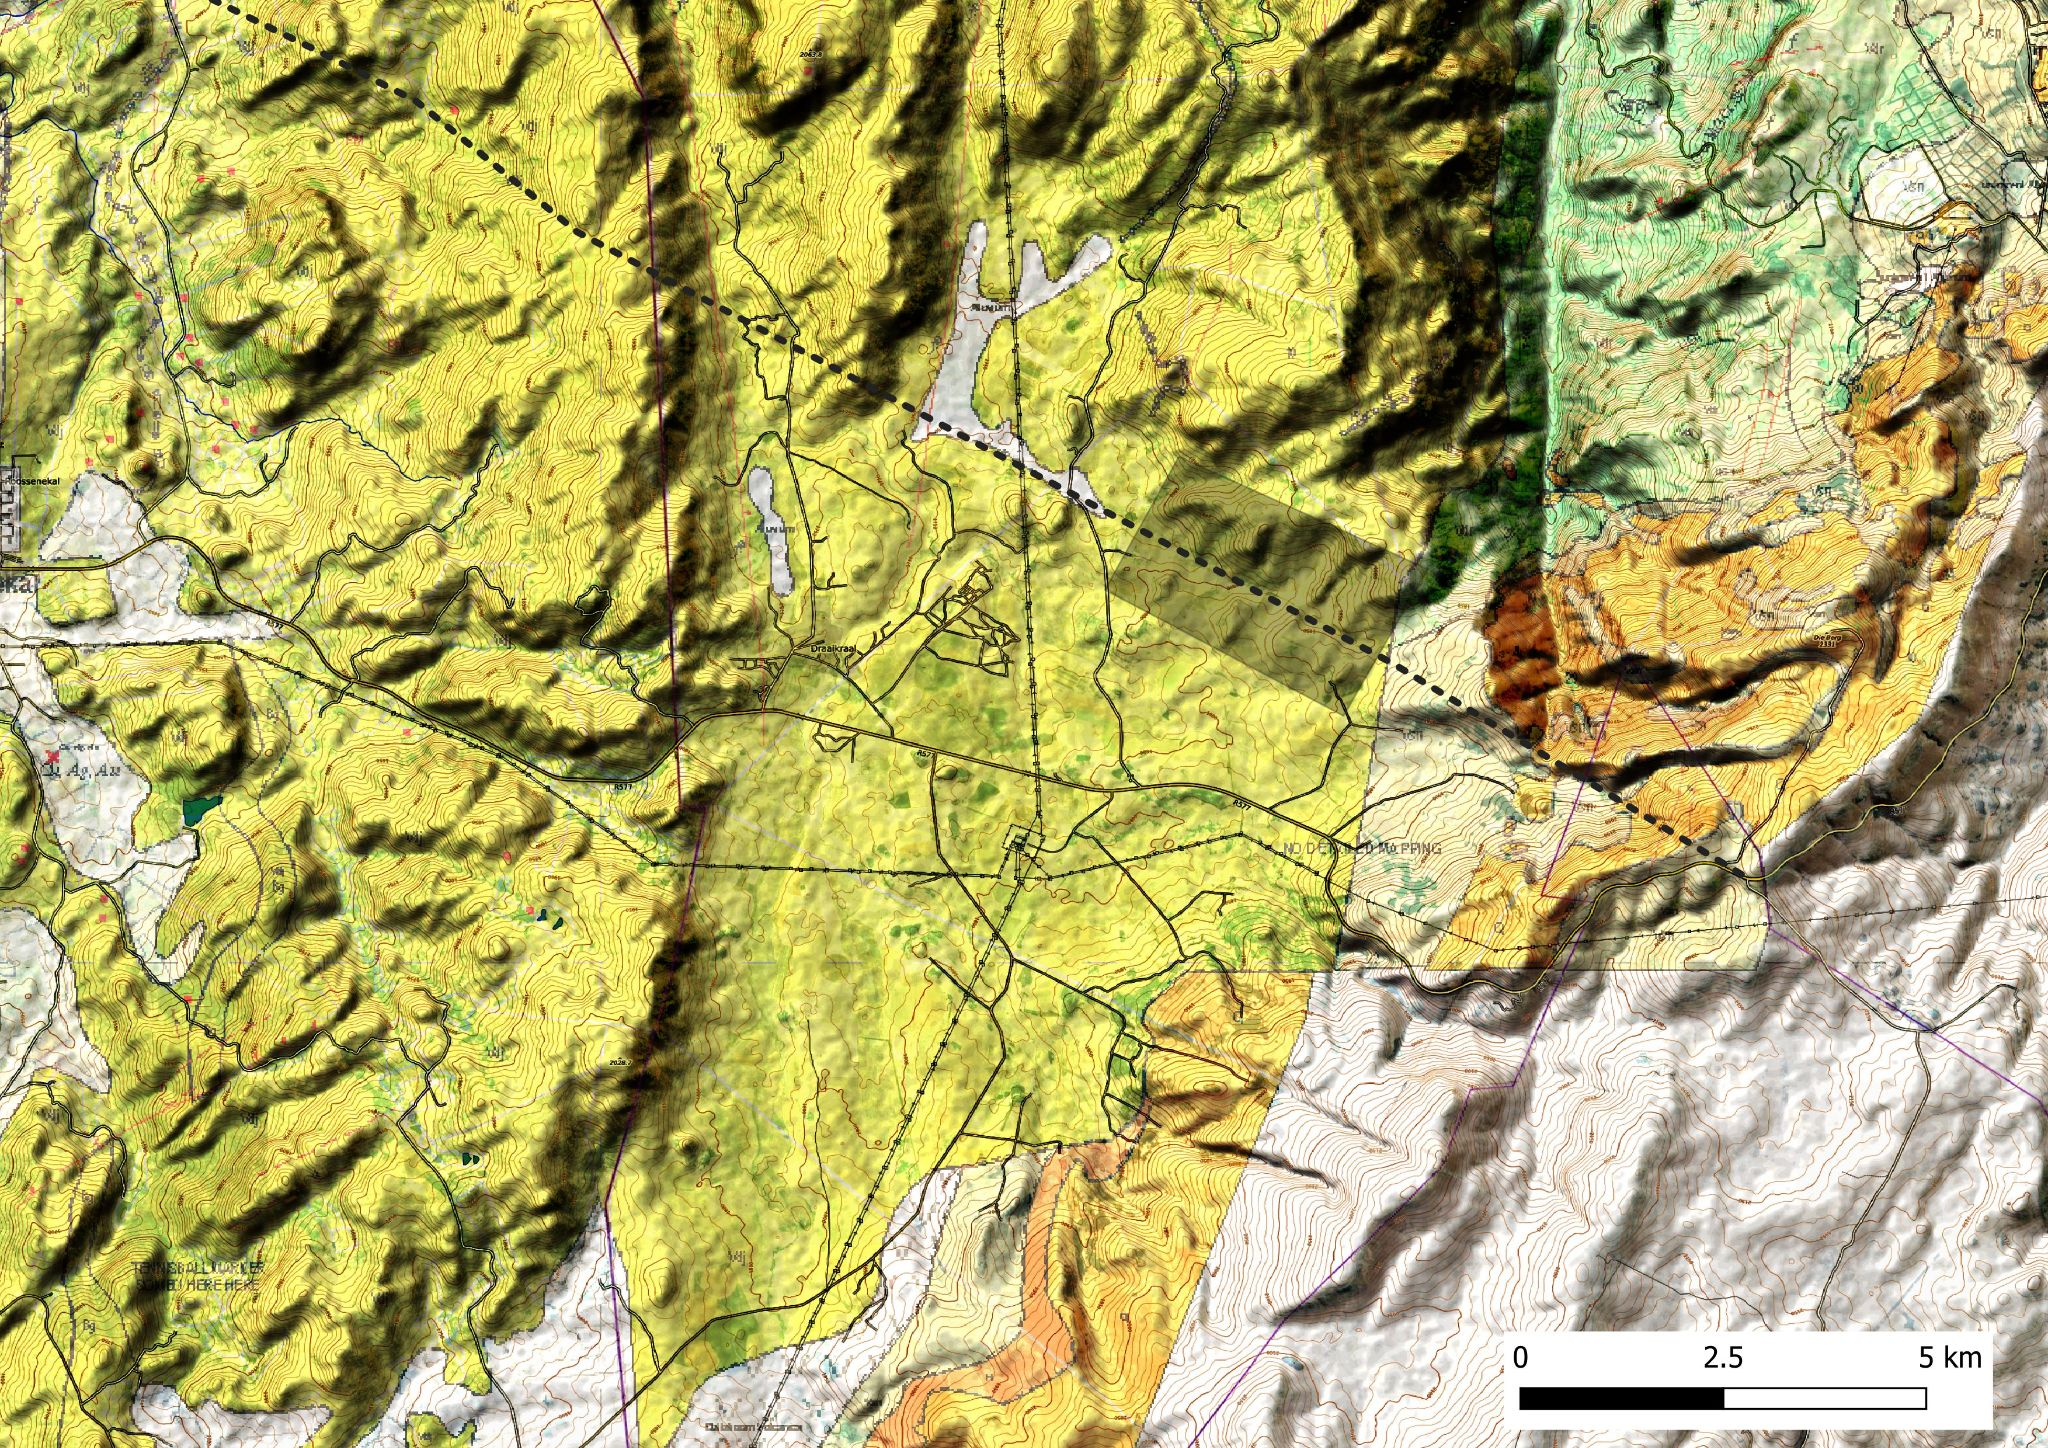
\includegraphics[width=\linewidth,height=0.45\textheight,keepaspectratio]{draaikraal_regional_geology_molyneux2008.jpg}
    \caption{}
    \label{fig:ch5-topo-map-geology}
  \end{subfigure}\hfill
  \begin{subfigure}[t]{0.495\linewidth}
    \centering
    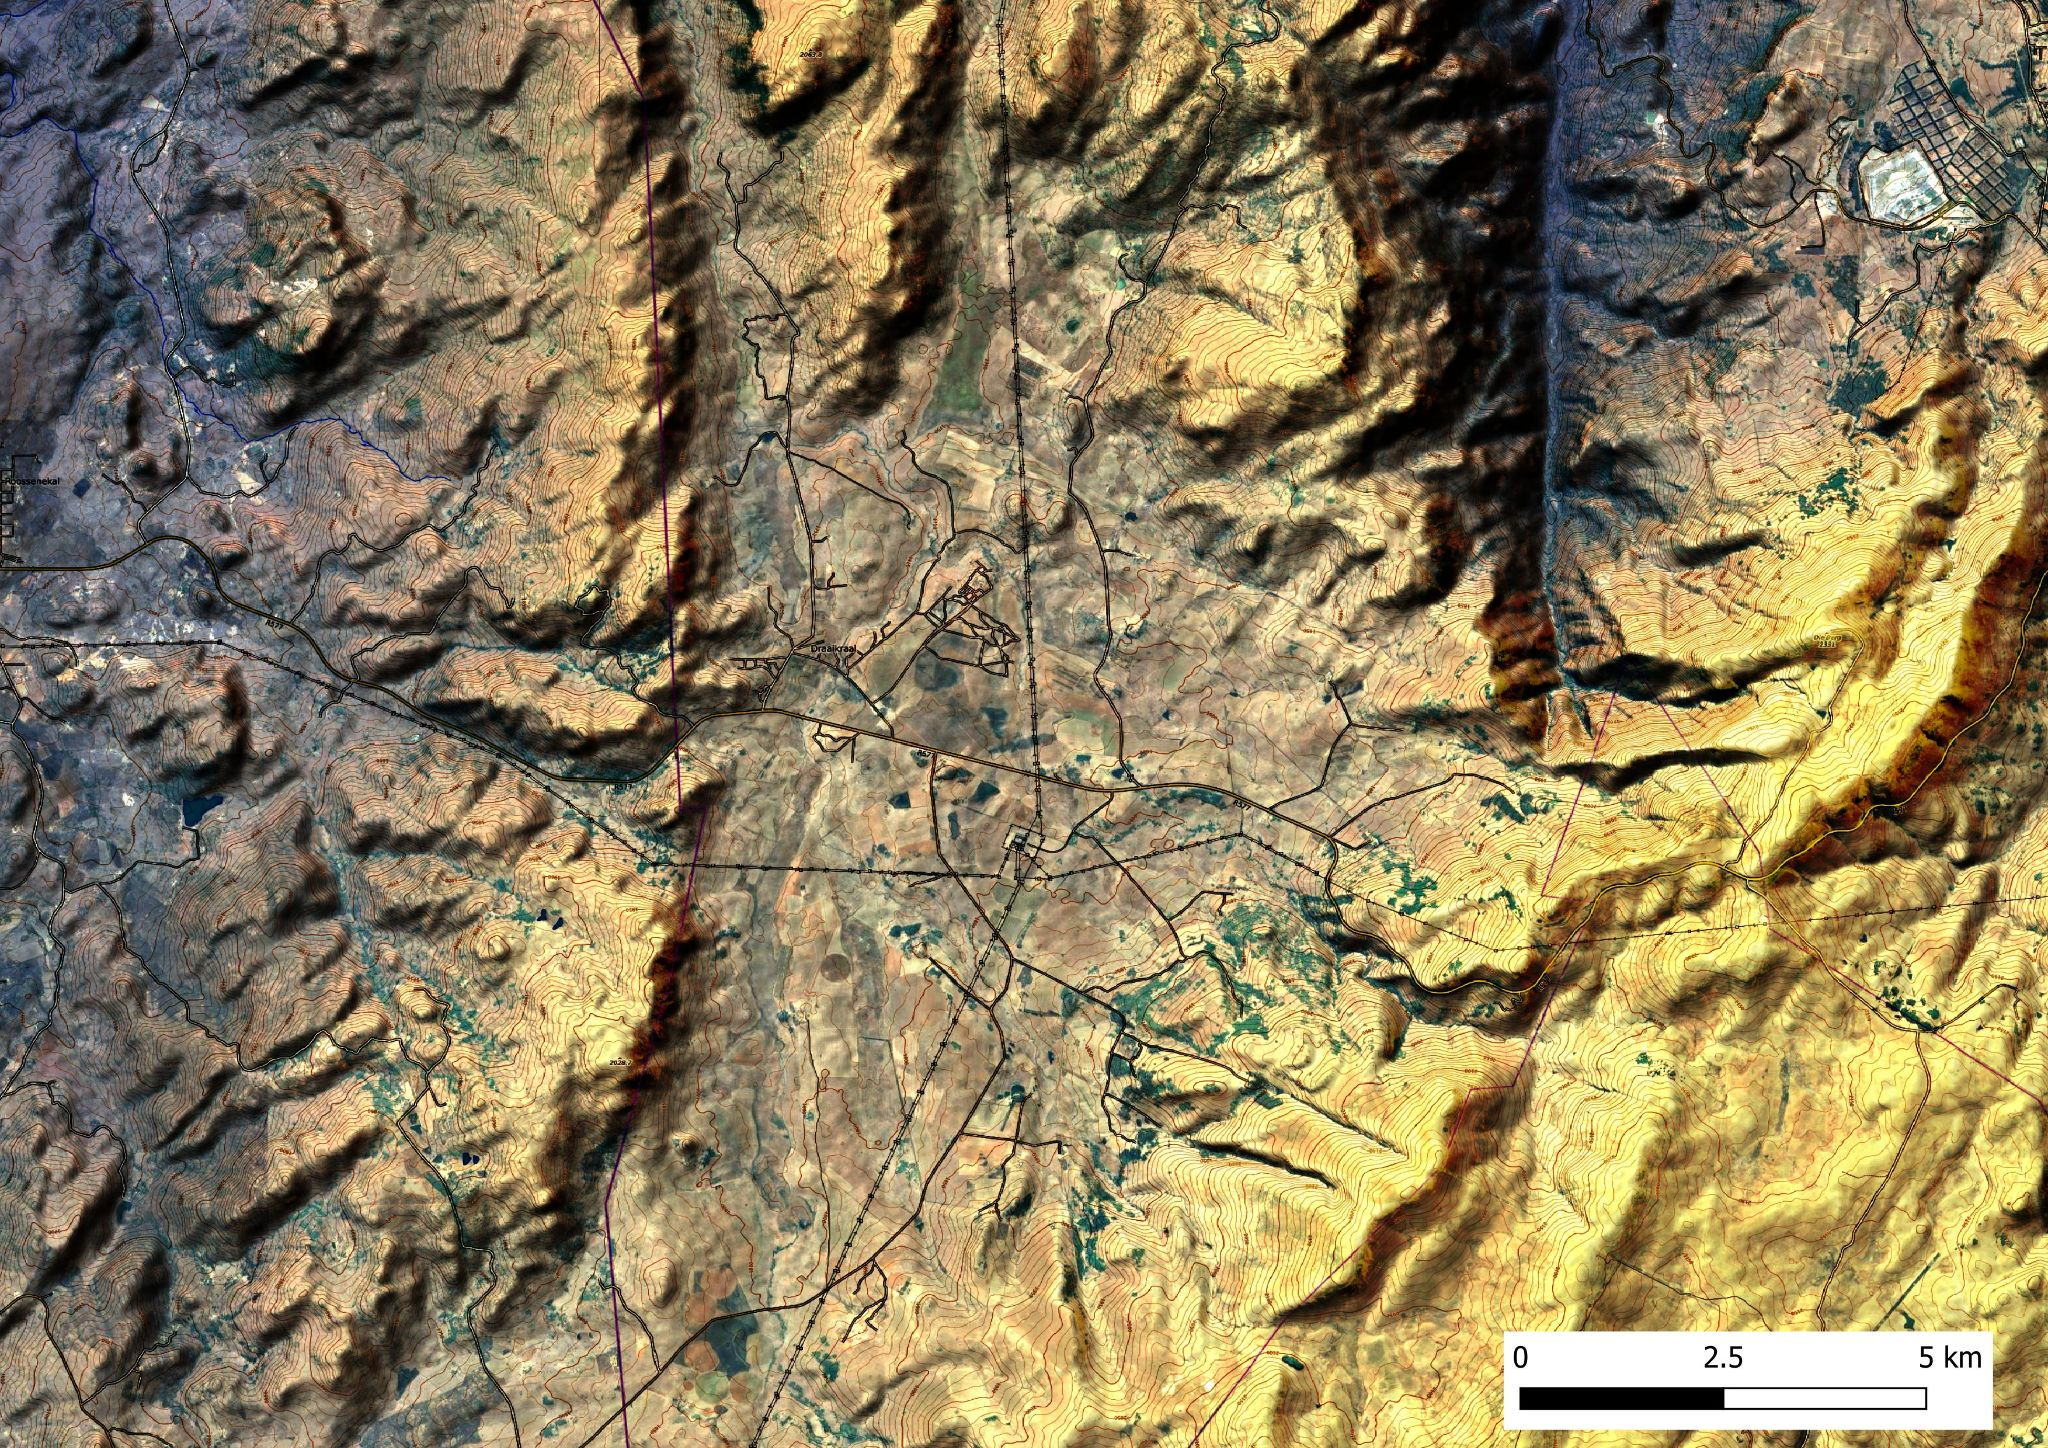
\includegraphics[width=\linewidth,height=0.45\textheight,keepaspectratio]{draaikraal_regional_topography_satellite.jpg}
    \caption{}
    \label{fig:ch5-topo-map-satellite}
  \end{subfigure}
  \caption{(a) The field area around Draaikraal with the geological mapping of
    \citet{molyneux2008}. Due North is up on this map. The generally resistant,
    topographically high Steenkampsberg Quartzite and hornfels are mapped as orange
    units on the eastern margin. The Marginal Zone is mapped as the beige color between
    the quartzite and the RLS. The Main Zone is featured in yellow, the Critical Zone in
    the NE quadrant is green and exhibits strikingly recessive topography. A regional
    SW-NE trending fabric is prominent, which agrees with all structural measurements of
    rock cleavage taken in the lower Main Zone and upper Critical Zone aside from the
    rotated units associated with the Kliprivier Synform. The dark box outlines an area
    where SW-NE rock fabrics appear continuous across the Draaikraal Lineament (dashed
    line). The Main Zone around Draaikraal is unusually recessive relative to the Main
    Zone north of the Draaikraal Lineament, or to the west. The compilation of
    \citet{molyneux2008} did not consider more recent mapping that revealed the presence
    of the Upper Critical Zone to the south, terminating beyond the map area
    \citep{vandermerwe2007}.
    (b) The satellite view of the same area as (a), without geology and visual guides
    for clarity. The Draaikraal Lineament remains clearly visible. Elevations are
    colormapped such that relative lows are blue and highs are yellow. The Main Zone is
    generally at higher elevation than the Critical Zone (in the northeast quadrant) and
    the Upper Zone (to the west), while the quartzitic Steenkampsberg Mountains in the
    southeast quadrant are locally the highest feature.}
  \label{fig:ch5-topo-map}
\end{figure}
\end{landscape}}

\section{Methods}
\label{sec:ch5-methods}


\subsection{Field Methods}
\label{sec:ch5-field-methods}
Field observations were made during an 11-day field campaign in July 2023. Field investigation and sampling strategies were
adapted as the study proceeded, but initially were focused on correlating distinct rock units across the Draaikraal Lineament and taking 
structural measurements on each side to characterize it. Geolocated samples were taken across the field area for later geochemical work. 
The observation that plutonic igneous rocks to the north of the Kliprivier Synform were highly unusual and distinct from those to the south
prompted a campaign to more thoroughly characterize its lithologic context and structure. Field observations, samples, and structural measurements
were all geolocated and are recorded in Table~\ref{tab:ch5-field-stations} (Appendix~\ref{app:draaikraal-field-data}). Almost every entry included an interpreted lithological unit to inform
the final geologic map of the area (Figure~\ref{fig:ch5-lithological-map}). Many entries included photographs, which included mostly
close-up photos of outcrops, but also some photos of the surrounding landscape to illustrate the area's geomorphology. Field photographs are cited 
throughout this chapter by number (e.g., photo~\ChFivePhoto{95}); the photographs that
are reproduced in the photo album of Appendix~\ref{app:draaikraal-field-data}
(\S\ref{sec:ch5-SI-photo-album}) are linked from their numbers, and the rest
are in the supplementary photo album. \todo{Link to photo supplement here.}


\subsection{Mapping Criteria}
\label{sec:ch5-mapping-criteria}

The contact between the layered series (Critical and Main Zones) and the
Marginal Zone is often gradational, requiring a somewhat arbitrary
categorization. Since the Lower Main and Upper Critical Zones are
non-magnetic and the finer-grained marginal zone rocks are magnetic, I chose
field-detectable magnetism as the simple discriminant to distinguish
marginal rocks from the massive Main and Critical Zones of the RLS. 

When Layered Gabbronorites (Lg) are
observed in the same outcrops as Mottled or Spotted Anorthosites, the
locality is assigned to be Mottled or Spotted Anorthosite.

\subsection{Structural Measurements}
\label{sec:ch5-structural-methods}

All measurements of plutonic rocks reported here are orientations of
near-planar rock cleavage (\S\ref{sec:ch5-cleavage-layering}).
Strike and dip measurements taken from the Kliprivier Synform were
plotted on a stereonet and analyzed using Stereonet 11 \citep{allmendinger2012,cardozo2013}. Poles to bedding planes of
quartzites, hornfels, mafic sills, and plutonic rocks were calculated
and plotted together in stereonet projection in Figure~\ref{fig:ch5-stereonets}a. In Figure~\ref{fig:ch5-stereonets}b,
the fold axis is calculated using the poles to the bedding planes. The axial plane also was calculated, assuming it
bisected the obtuse angle formed by the limbs. The obtuse fold angle
bisector for the axial plane was selected because the rotation within
the fold observed is quite gentle. An acute bisector for the axial plane
would have been better supported if field evidence showed dramatic changes
in dip along the fold, requiring a complete structural overturn that
locally annihilated the original horizontality of the deformed rocks in
addition to steeply dipping rocks intermediate to the two limbs.

\subsection{Stratigraphic Column Analytical Methods}\label{sec:ch5-stratigraphic-column-methods}

The field data of this study north of the Kliprivier Synform are
projected onto a stratigraphic column following the assumption that all
rocks in the field area north of the Kliprivier Synform follow
Steno's Law of Original Horizontality and were only uniformly deformed
by tilting due to isostatic flexure towards the center of the RLS after
emplacement, so that all regional bedding and structures are currently
dipping 15 degrees to the northwest relative to their original
orientations. Geolocated field data are projected onto a line to the north of the
Kliprivier Synform designed to be orthogonal to the regional strike
(trending 301.79 degrees: W-NW) using the `Snap Geometries to Layer' function in
the `Vector Geometry' Processing Toolbox in QGIS, with a tolerance of 1
degree set to ``prefer closest point''. Section heights then were calculated for
these projected points along the reference line to an arbitrary point along this line,
to get relative stratigraphic heights using the  ``Distance Matrix'' function 
in the ``Vector Analysis'' Processing Toolbox. A correction was added to these lateral distances to
account for elevation, calculated as the product of the elevation
differential and the tangent of the regional dip, assumed to be 15°. The
column heights are normalized to the height of the Merensky Reef. Because
the Merensky Reef was not observed in the field area, this was instead done by proxy: stratigraphic heights were
calculated relative to the UG2 chromitite observed in the field area (\S\ref{sec:ch5-unit-ug2}) at a fixed height of -86 meters. 
This chromitite is mapped by \citet{vandermerwe2007} as the UG2, who profiled drill cores 
and determined the Merensky Reef to be 86 meters above the UG2 in the field area \citep{vandermerwe2007}. Note that, for simplicity, 
it is assumed that there are no local changes in strike and dip,
even though the dip of the Main Zone likely shallows and rotates to be
roughly due east further from the margin of the intrusion. This approximation is likely to be acceptable locally for the upper 
Critical and lower Main zones, but becomes less accurate further from the margin. Therefore, the
stratigraphic heights presented here for the Homogeneous Gabbronorite
lithology far upsection are likely overestimated. The interpreted schematic
stratigraphic column for the region is graphically presented in
Figure~\ref{fig:ch5-strat-column}.

\begin{figure}[htbp]
  \centering
  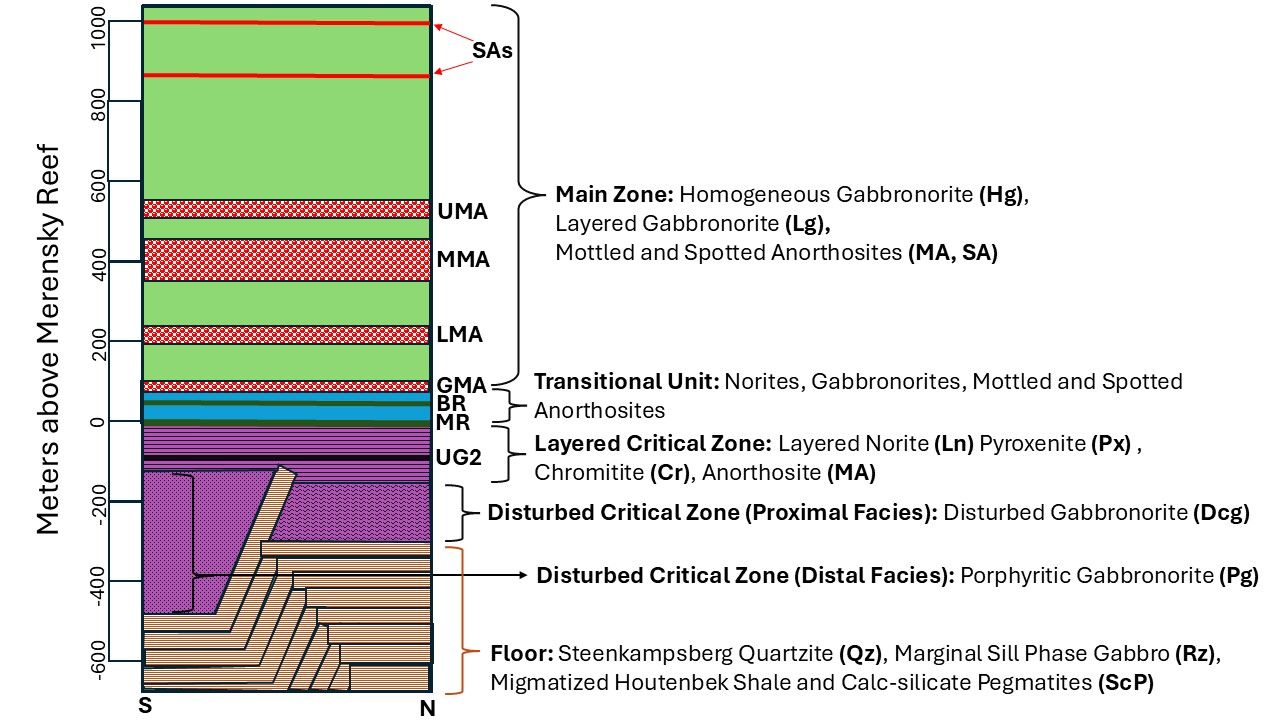
\includegraphics[width=\linewidth]{draaikraal_schematic_strat_section.jpg}
  \caption{The schematic stratigraphic cross section of the RLS in Draaikraal. The
    Kliprivier Synform is represented by the slab of floor rocks protruding into (and
    creating) the Disturbed Critical Zone at the halfway point of the column. The
    Draaikraal Lineament would form from upward percolating fluids trapped and channeled
    by this protruding slab of floor rocks in a line directly above the slab in this
    view. The Kliprivier Synform is not interpreted to have deformed the RLS above the
    UG2.}
  \label{fig:ch5-strat-column}
\end{figure}

\section{Results: Field Observations}
\label{sec:ch5-field-observations}

Observations are organized into three sections: lithologic descriptions, rock cleavage and modal layering, and structural observations; the first and last each have their own map.

\subsection{Lithologic Descriptions}
\label{sec:ch5-lithologic-descriptions}

Lithologic descriptions are organized by the interpreted map units (see Figure~\ref{fig:ch5-lithological-map}) and their constituent lithologies. 
Three mapping units are described in turn, each with a wide variety of lithologies: the marginal rocks (the floor and walls of the intrusion, 
including sedimentary country rock and concordant pre- and syn-Bushveld magmatic sills); the plutonic rocks of the RLS;
and secondary, post-Bushveld rocks that were largely ancillary to the field study. 

\afterpage{%
\begin{landscape}
\begin{figure}[p]
  \centering
  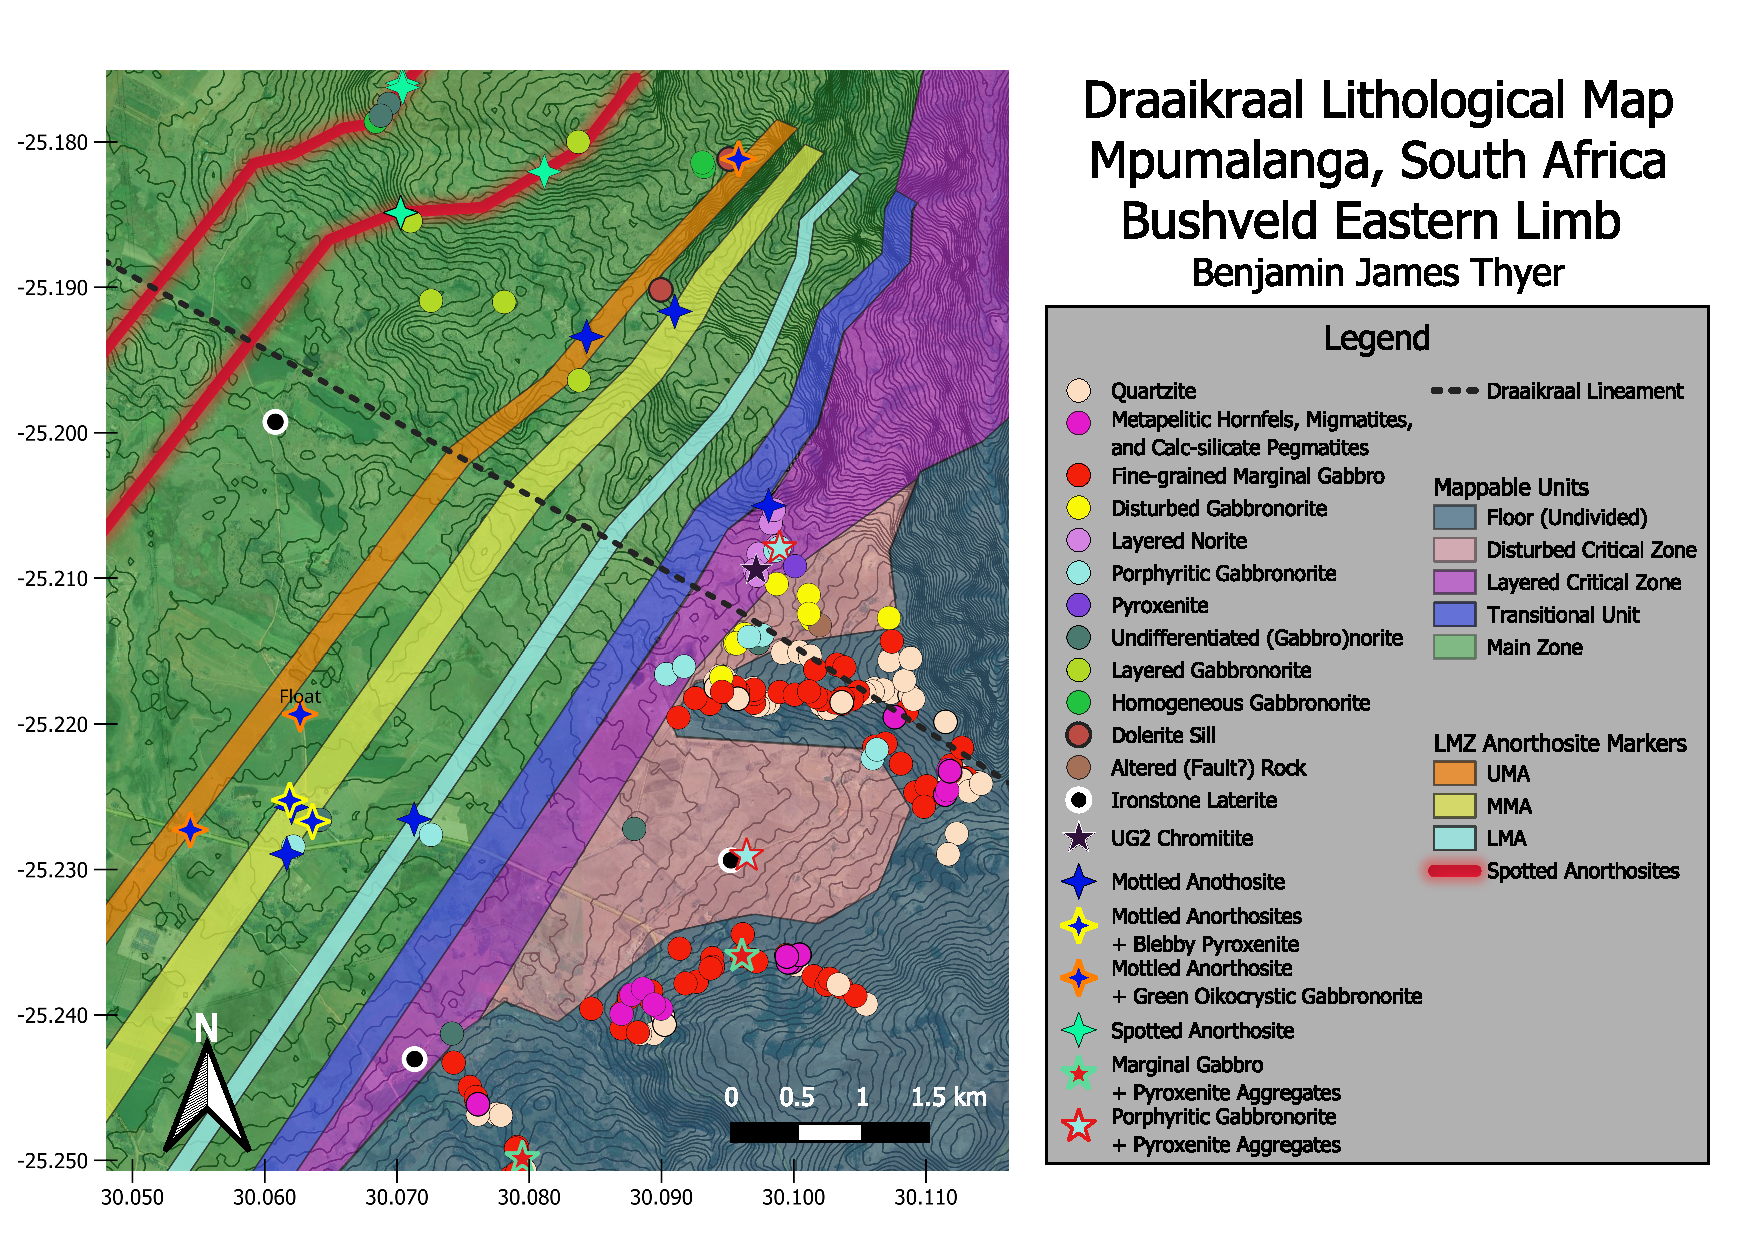
\includegraphics[width=\linewidth,height=0.8\textheight,keepaspectratio]{lithological_map.pdf}
  \caption{Lithological map of the Draaikraal field area, eastern limb of the Bushveld
    Complex. Field observations of outcrop are colored by lithology over the mappable units (floor,
    Disturbed Critical Zone, Layered Critical Zone, Transitional Unit, Main Zone). The
    lower Main Zone anorthosite marker beds (LMA, MMA, UMA, and the spotted
    anorthosites) are traced in color, and the Draaikraal Lineament is dashed. Field observation
    data are listed in Table~\ref{tab:ch5-field-stations}.}
  \label{fig:ch5-lithological-map}
\end{figure}
\end{landscape}}

\subsubsection{Margin}
\label{sec:ch5-eastern-margin}

Much of this study focused on the eastern margin of the eastern limb of
the Rustenburg Layered Series (RLS) east of Draaikraal. The margin
displays the most unambiguous bedding planes of the study area,
generally dipping 25° to the northwest towards the center of the
Bushveld Complex, except for the Kliprivier Synform, which is detailed
below in the \hyperref[sec:ch5-structural-observations]{``Structural Observations''} section. The marginal rocks
within the field area are composed of gabbroic intrusive igneous sills
concordantly intercalated with variably metamorphosed, melted, or
otherwise devolatilized Transvaal sediments of the Steenkampsberg and
Houtenbek formations. Occasionally, melting and/or reactive porous flow
of melts through sedimentary layers remineralizes sedimentary layers
with igneous mineralogy and texture (photos~\ChFivePhoto{35}, \ChFivePhoto{51}, and \ChFivePhoto{52}). Concordant
sills of marginal zone magmas and packages of sediment range in
thickness from 10 to 100s of meters, and can be found mutually
interbedded at least a kilometer from the margin of the RLS. Here, the
marginal rocks are divided into three units: ``Rz'', the fine-grained
Marginal Zone gabbroic sills/magmas; ``Qz'', relatively undisturbed
Houtenbek quartzite; and ``ScP'', hornfelsed metapelites, marbles, and
quartzites with related igneous/hydrothermal pegmatites.

\subsubsection{Rz -- Fine-grained gabbro}
\label{sec:ch5-unit-rz}

The Marginal Zone gabbroic sills are commonly fine grained (\textless1
mm), but locally are coarser with some grains up to 2 mm in the
groundmass. Unlike much of the plutonic RLS, the Marginal Zone is not
visibly modally layered. Marginal Zone magmas within a meter of
Steenkampsberg Quartzite often contain conspicuous evidence of silicic
contamination: although they retain an igneous texture, the color
significantly lightens and the rocks become much harder and less
magnetic approaching the contacts with Steenkampsberg Quartzite. Aside
from these immediate contacts, the Marginal Zone gabbro is always
magnetic. The Marginal Zone contains more pyroxene (distinguishing
clinopyroxene and orthopyroxene is difficult with such small crystals)
than plagioclase with variable magnetite, sometimes up to 10\%, and
minor phlogopite. The heavy, fine fraction of mineral separates from one
sample was briefly studied under optical microscope to identify trace
phases, which include apatite, zircon, sulfides, and euhedral chromite.

The Marginal Zone magmas contain igneous xenoliths and are rich in
paleo-vertical, across-strike features that likely record rising,
buoyant fluid/magma. Perfect planar resistance banding (photo~\ChFivePhoto{95}) is the
most common structure in the fine grained Marginal Zone and is nearly
ubiquitous within the unit. Though the resistance bands have seemingly
random strikes, they most often are steeply dipping and may represent
fluid conduits along brittle fractures within the Marginal Zone.

In previous works, isolated meta-sedimentary xenoliths \citep{buick2000}
were emphasized, but in this study, meta-sedimentary rocks were
never found as minor xenoliths within magnetic marginal sills, but
rather as continuous, concordant strata (photos~\ChFivePhoto{42}, \ChFivePhoto{70}, \ChFivePhoto{71}) or as
locally abundant disaggregated broken strata cemented within a pink,
evolved diatexite (photo~\ChFivePhoto{100}), both designated as a distinct unit: ScP.

The magnetic sills of the Marginal Zone (Rz) did include enclaves of
coarse-grained leucogabbronorite, mottled anorthosite or pyroxenite
(photos~\ChFivePhoto{2},\ChFivePhoto{4},\ChFivePhoto{6},\ChFivePhoto{96}). The anorthosite-rich enclaves are rounded, 6-10 cm
along their longest dimension, and are imbricated to be preferentially
lying flat paleohorizontally within the Marginal Zone, suggesting they
were weathered/eroded by reaction and/or mechanical transport through
Marginal Zone magma. Pyroxenitic enclaves are also often spherical
(photos~\ChFivePhoto{4}, \ChFivePhoto{96}) and may be related to the formation of the pyroxenite
``Tennis Ball Marker'' (TBM) of the Main and Critical Zones, described
further in the discussion. These plagioclase-rich igneous xenoliths
contain large (\textless3 cm) optically continuous oikocrystic augite
that enclose blocky plagioclase (\textless5 mm).

More commonly observed within the magnetic Marginal Zone sills east of
Draaikraal are paleovertical structures that suggest buoyant upwelling
of fluids and melts sourced from the hornfelsized sedimentary rocks.
These structures included sheared, viscously deformed lenses of
thin pegmatites, including anorthosite (photo~\ChFivePhoto{6}), magnetite gabbros
(photo~\ChFivePhoto{60}, sheared gabbro \textasciitilde{}15 cm;
Figure~\ref{fig:ch5-photo60-deformation}), and evolved
quartz-biotite pegmatites (photo~\ChFivePhoto{67}: 1$\times$3~cm). In addition to homogeneous
pegmatites, the Marginal Zone gabbros host paleovertical invasions of
anastomosing anorthosite derived from anatexis of underlying
metasedimentary rocks (photos~\ChFivePhoto{6}, \ChFivePhoto{97}). These leucosome intrusions
occasionally carry blocks of meta-sedimentary paleosome or brecciate and
enclose the Marginal Zone gabbronoritic host rock itself (photo~\ChFivePhoto{98}).

Near the contact with the migmatite, differential weathering sometimes
reveals proud, thin, pinched ovate paleovertical structures (5$\times$1~cm
scale) on weathered faces of Marginal Zone norite that are otherwise
invisible on a fresh rock face {[}photo~\ChFivePhoto{40}{]}.


Fine-grained Marginal Zone gabbros are mapped up to 120 meters below the
Merensky Reef stratigraphically.

\subsubsection{Qz -- Houtenbek Quartzite}
\label{sec:ch5-unit-qz}

The Houtenbek quartzite dips concordantly with marginal zone sills and
migmatized sedimentary rocks towards the center of the Bushveld, here
dipping about 25° to the northwest. Even within meters of a contact with
Marginal Zone sills (Rz), the quartzite often retains a clastic
sedimentary texture and possibly could be considered a proper
clast-dominant quartzose sandstone with well-sorted and well-rounded
coarse quartz grains \textasciitilde1 mm in diameter with no other
mineral visible. While there is little structure visible internally
because of the purity of the quartzite, the bedding planes occasionally
reveal conspicuous asymmetric ripple structures {[}photos~\ChFivePhoto{2}, \ChFivePhoto{68}{]}
\textless1 cm in height. One in-place ripple structure suggests a
paleoflow direction towards the south-southwest. Some quartzites are
hornfelsized: recrystallized into an interlocking crystalline texture
with large, irregular, angular, coarse grains \textless2 cm across. Many
quartzites with preserved clastic textures near the margin of the RLS
are stained bright red within rocks' unweathered interior. This staining
is hypothesized to be derived from mobilized Fe-rich fluids percolating
along grain boundaries, probably caused by heat and/or fluid circulation
related to the emplacement of the RLS. Steenkampsberg Quartzite is mapped
up to 140 meters below the Merensky Reef stratigraphically.

\subsubsection{ScP -- Houtenbek Hornfels, Migmatites, Pegmatites}
\label{sec:ch5-unit-scp}

In addition to quartzite, the Houtenbek formation contains carbonate and
pelitic horizons \citep{button1976}. At the margin east of Draaikraal, there
is a 60 m thick package of melted and metamorphosed sediment containing
stratiform pegmatites with variable mineralogy. Hornfelsized sediments
come in two main varieties near Draaikraal: pink, diatexite-supported
breccias {[}photo~\ChFivePhoto{100}{]} or dark, high-grade schists {[}photo~\ChFivePhoto{29}{]} with
thin but conspicuous navy, gray, white, tan, and pink bands of
relatively mafic and felsic minerals that have been recrystallized and no
longer bear clastic textures except for thin seams of clast-dominated
quartzite in a low-fraction glassy biotite-rich matrix {[}photo~\ChFivePhoto{35},
large light seam is \textasciitilde4 cm thick{]}. This unit is rarely
magnetic and most often is visible as continuous, concordant strata
{[}photo~\ChFivePhoto{42}{]}. Even when highly brecciated, this unit can be followed
along the strike of the quartzites and Marginal Zone, implying that the
sediments were not incorporated into Marginal Magmas, but that they
rather were melted and devolatilized in-situ due to heating from the
emplacement of adjacent marginal sills. Fluids and melts produced in
this process are visible as a wide variety of stratiform pegmatites and
skarns with undulating erosive contacts within comparatively planar
meta-sediments {[}photo~\ChFivePhoto{30}: feldspar/wollastonite(?) + amphibole skarn;
photo~\ChFivePhoto{69}: magnesite, quartz pegmatite with minor siderite{]} and as
pockets following fluid flow pipes and void spaces that are accommodated
by the host strata through ductile deformation {[}photo~\ChFivePhoto{37}, \ChFivePhoto{38}:
Orthopyroxene and quartz pegmatite{]}. Hornfels in the field area are
mapped up to 190 meters below the Merensky Reef stratigraphically.

\subsubsection{The Rustenburg Layered Series (RLS)}
\label{sec:ch5-rls-units}

The Rustenburg Layered Series is the world's largest individual igneous
intrusion \citep{cawthorn2015,latypovetal2022} and is subdivided into the Lower Zone, Critical Zone, Main Zone, and Upper Zone (\S\ref{sec:ch5-the-bushveld-event-and-rls}). In this study, RLS
rocks of the lower Main Zone, Transitional Zone, and upper Critical Zone
are mapped. The rocks of the Marginal Zone (Rz) are not layered, nor
considered here to be a part of the RLS on a textural basis. Marginal
zone rocks weather distinctly from the plutonic RLS phase with abundant,
sharp, \textasciitilde3 cm-scale potholes and generally are more
textured and rough {[}photo~\ChFivePhoto{36}{]} on a weathered surface than RLS rocks,
which weather spheroidally and proudly {[}photos~\ChFivePhoto{8}, \ChFivePhoto{11}: ``porphyritic''
gabbronorite{]}. Xenolith blocks of Marginal Zone norites bearing their
distinctive resistance banding are found in both the Critical and the
Main Zones {[}Critical Zone: photo~\ChFivePhoto{76}; Main Zone: \ChFivePhoto{91}{]}, though each
xenolith sighting within the Main Zone is proximal to a mottled or
spotted anorthosite layer. These xenoliths are variably annealed,
recrystallized, and even ductily deformed {[}Critical Zone: photo~\ChFivePhoto{77};
Main Zone: \ChFivePhoto{84}{]}.

The RLS is famous for its distinctive and numerous laterally continuous
stratiform marker horizons, sometimes stretching on a 100-km scale
\citep{cawthorn2015}, which include the Critical Zone chromitite cycles,
Merensky and Bastard pegmatoid reefs, three mottled anorthosite packages
in the lower Main Zone, the Pyroxenite Marker of the upper Main Zone,
and the magnetitite cycles of the Upper Zone. In this study, I observe
and describe the three lower Main Zone magnetic mottled anorthosites
{[}photos~\ChFivePhoto{49}, \ChFivePhoto{53}, \ChFivePhoto{86}, \ChFivePhoto{93}, \ChFivePhoto{105}, \ChFivePhoto{106}, \ChFivePhoto{108}, \ChFivePhoto{111}{]}, the magnetic chromitite
UG2 {[}photos~\ChFivePhoto{65}, \ChFivePhoto{66}{]}, and a non-magnetic upper Critical Zone mottled
anorthosite that is probably a part of the Merensky Reef footwall
{[}photo~\ChFivePhoto{81}{]}, and several packages of xenolith-bearing modally layered
gabbronorites and spotted anorthosites within the Main Zone (photos~\ChFivePhoto{91} and \ChFivePhoto{111}).
These laterally continuous reefs are mapped and described separately
from the bulk cumulate rocks of the RLS.

\subsubsection{Cz: Critical Zone}
\label{sec:ch5-zone-cz}

The Critical Zone was previously mapped to pinch out due east of
Draaikraal \citep[shown in the compilation of][]{molyneux2008}; however,
many now recognize that a thin layer of the upper Critical Zone persists
much further south towards Tontledoos \citep{vandermerwe2007}. In this
study, diagnostic Critical Zone lithologies were only observed north of
the Kliprivier Synform, where typical finely modally layered norites
and anorthosites are well-exposed (photos~\ChFivePhoto{64} and \ChFivePhoto{80}), as well as the UG2
chromitite. The Critical Zone above the Kliprivier Synform dips
\textasciitilde15° to the northwest similarly to the majority of the
Main and Marginal Zone rocks in the field area, but gradually rotates to
a southwestern dip as it approaches the contact with the rotated block
of metasediments and gabbronorite sills of the Kliprivier Synform. It is
essential to note that some rotated Critical Zone rocks are structurally
beneath the large, rotated package of intruded metasediments (Rz + Qz +
ScP) in the area of the Kliprivier Synform, meaning that this package of
country rock is not only serving as the floor for RLS rocks to the west,
but is also (at least locally) a roof for Critical Zone rocks below the
level of the UG2.

\subparagraph{Dcg: Disturbed Gabbronorite}
\label{sec:ch5-unit-dcg}

This lithology is restricted to the immediate area of the Kliprivier
Synform. Disturbed Gabbronorites are coarse-grained, even pegmatoidal
(photo~\ChFivePhoto{62}), with feldspars and pyroxenes up to 3~cm long. This unit was
named in response to \citet{vandermerwe2007}, who said that the
``structural change {[}of the Kliprivier Synform{]} is reflected in the
Bushveld rocks, which become highly disturbed and fragmented''.
Disturbed Gabbronorites are most recognizable for their abundance of
blobby autoliths of anorthosite (photo~\ChFivePhoto{61}) and pyroxenite (photos~\ChFivePhoto{70} and
\ChFivePhoto{72}). While it exhibits abundant examples of modal separation, they are
never remotely planar, unlike the majority of the RLS. 

This lithology is most often non-magnetic, but a few specimens were
magnetic. Besides the mottled anorthosites of the Main Zone and the
anorthosite-hosted chromitite leader of the UG2, no other rocks of the
RLS within the field area are magnetic. Many but not all Disturbed
Gabbronorites are rotated within the Kliprivier Synform. Generally, the
Disturbed Gabbronorites are CPX-poor and sulfide-rich with abundant,
euhedral \textless1 cm pyroxenes set in an anorthosite matrix that
effectively isolates the large, euhedral pyroxenes from one another
{[}photo~\ChFivePhoto{62}{]}. This unit generally becomes more feldspathic as one
moves away from the intruded metasediments of the Kliprivier Synform
into the Critical Zone. This lithologic unit contains recrystallized and
annealed xenolith blocks {[}photos~\ChFivePhoto{74}, \ChFivePhoto{75}, and \ChFivePhoto{77}{]} of fine-grained
Marginal Zone gabbros (Rz) as well as coarse-grained pockets containing
very large (\textless{} 5cm) oikocrystic pyroxene {[}photo~\ChFivePhoto{73}{]} and
large clusters of pyroxene often rimmed by thick anorthosite halos
{[}photo~\ChFivePhoto{72}{]}. Disturbed Gabbronorite is mapped between 120-145 meters
below the Merensky Reef stratigraphically, around the level of the UG1
in core logs \citep{vandermerwe2007}. \citet{vandermerwe2007} and
\citet{latypovetal2022} report isolated patches of massive chromite here, but I did
not see any.

\subparagraph{UG2: Upper Group 2 Chromitite}
\label{sec:ch5-unit-ug2}

Near the top of the upper Critical Zone in the extreme northern portion
of Kliprivier farm, there is a small but high-quality exposure of
chromitite (\textgreater30 cm thick). The bulk of the exposure is a
melanocratic, non-magnetic, anorthositic chromite, which is modally
\textasciitilde50\% \textless1mm euhedral chromite set within a fine
matrix of \textless1 mm plagioclase (photo~\ChFivePhoto{66}). Structurally above this
massive layer are some thin (\textless1 cm thick) chromitite leaders
hosted within bright white mottled anorthosite (photo~\ChFivePhoto{65}). Both layers
contain amoeboid oikocrystic pyroxene-olivine mottles (\textless2cm).
The mafic silicate mottles and anorthosite matrix seem to have
crystallized within the interstices of a preexisting framework of a
continuous chromite crystal slurry {[}photos~\ChFivePhoto{65}, \ChFivePhoto{66}{]}, \citep[see][for similar interpretations]{voordouw2009,mukherjee2017}. The
massive melanocratic layer includes pure (relatively chromite-free)
white anorthosite blocks (\textless4$\times$15~cm) that are lying flat and
dipping west towards the center of the Bushveld Complex. These pure
anorthosite blocks contain thin chromitite stringers that together have
been ductilely deformed, and a thin (\textasciitilde1 mm) white seam of
pure, apparently undeformed anorthosite forms a plane bounding the top
of some of these blocks, also dipping to the west.

The anastomosing chromite leaders within the overlying mottled
anorthosite are sometimes highly magnetic and are a much deeper,
vitreous black: appearing under hand lens to be \textgreater80\% modally
chromite/magnetite {[}photo~\ChFivePhoto{65}{]}.

This chromitite package is interpreted as UG2 for a few reasons. First,
although the anastomosing chromite leader resembles the UG1 stringers,
the leader is structurally above the massive chromitite, whereas the UG1
stringers are recognized below the massive chromitite \citep{voordouw2009,mukherjee2017}. The UG2 is known to have several small
``leaders'' a small distance above the main seam \citep{maier2024}. Second, the magnetic chromitite within the leader bears
explaining. One heterogeneous magnetic chromitite at the top of the UG2
with discrete magnetic and non-magnetic bands was described by
\citet{frankel1942}, 20-30 km to the north of Kliprivier at Tweefontein.
Third, a rock at this location was also mapped as the UG2 by \citet[Fig.~4]{harmer1985} and \citet[Fig.~3]{vandermerwe2007}, who also
identified the UG2 and closely overlying mottled anorthosites in drill
cores of the area using PGE grades. \citet{vandermerwe2007} also reports
that the UG2 at Kliprivier is unusually enriched in iron, which may
explain the magnetism of the leader. The UG2 is 86 meters below the
Merensky Reef in the direct vicinity of the Kliprivier Synform \citep[Borehole~3:][]{vandermerwe2007}.

\subparagraph{Ln: Layered Norite:}
\label{sec:ch5-unit-ln}

Spectacular outcrops of modally layered norites within the upper
Critical Zone are observed within the field area at Kliprivier around
and above the stratigraphic level of the UG2 chromitite (photos~\ChFivePhoto{64} and
\ChFivePhoto{80}), at stratigraphic heights from 100 to 50 meters below the Merensky
Reef. Modal layering is pronounced, with pyroxenite-rich layers being
separated by near-pure centimetric anorthosite bands. This layering is
undulose and irregular.

\subparagraph{Px: Pyroxenite}
\label{sec:ch5-unit-px}

This refers to rocks predominantly composed of pyroxenes. Pyroxenites
are rare in the field area. There was one coarse-grained sulfide-bearing
feldspathic pyroxenite horizon in the Critical Zone just below the UG2
(photo~\ChFivePhoto{78}) as well as a pyroxenite layer just below a mottled
anorthosite layer in the UMA in the lower Main Zone (photos~\ChFivePhoto{53}--\ChFivePhoto{54}).

\subsubsection{Tz: Transitional Zone}
\label{sec:ch5-zone-tz}

There is no perfect division for the Main and Critical Zones. Moving
upsection from the Critical Zone into the Main Zone, Cr\textsubscript{2}O\textsubscript{3} concentration within OPX decreases, strontium isotopes become more
radiogenic, and cumulus clinopyroxene becomes important--- but these
changes occur at different stratigraphic heights within the transition
zone \citep{cawthorn2015} between the Merensky Reef and Giant Mottled
Anorthosite (or above). Within the literature, the bottom of the Main
Zone is considered to be above the Giant Mottled Anorthosite at the top
of the Bastard unit, and the Merensky reef is taken to be the top of the
Upper Critical Zone \citep{cawthorn2015,mitchell2002,vandermerwe2007}. The Bastard and Merensky pyroxenites and Giant Mottled
Anorthosite were never observed in the field area, but a
\textasciitilde50 cm thick mottled anorthosite {[}photo~\ChFivePhoto{81}{]} was
observed \textasciitilde50 meters upsection from the UG2 with only
finely layered norite {[}photo~\ChFivePhoto{80}{]} and porphyritic gabbronorite
outcropping between the UG2 and the mottled anorthosite. Since
\citet{vandermerwe2007} reports in core logs that the Merensky Reef is 86 meters
above the UG2 on Kliprivier and \citet{latypovetal2022} observe unusual
pyroxenites just above this mottled anorthosite, this anorthosite layer
is interpreted to be a part of the footwall to the Merensky Reef, and
the pyroxenites described in \citet{latypovetal2022} are interpreted to be
the Merensky Pyroxenite.

\subparagraph{Pg: Porphyritic Gabbronorite}
\label{sec:ch5-unit-pg}

The ``Porphyritic Norite'' is a well-recognized marker of the lower Main
Zone, with large, rounded pyroxene phenocrysts set in a white,
feldspar-rich matrix, used often in mining to locate the Merensky Reef
\citep{sacs1980,vongruenewaldt1985}. I observe a general textural
similarity in lower Main Zone Gabbronorites with the unlayered upper
Critical Zone gabbronorites below the Merensky Reef (photos~\ChFivePhoto{10}, \ChFivePhoto{79}).
These gabbronorites are distinct from the dark and homogeneous
gabbronorites that compose the majority of the Main Zone (Hg). The
porphyritic gabbronorite contains large (\textasciitilde\textless{} 1cm),
equant pyroxenes set in a leuconoritic matrix that is predominantly
plagioclase with small spots of interstitial orthopyroxene. I refer here
to them collectively as the ``porphyritic gabbronorite'' because I see
cumulus clinopyroxene present throughout, becoming more modally abundant
upsection until about half of the cumulus pyroxenes are CPX near the
Lower Mottled Anorthosite (LMA). Generally, cumulus CPX is present in
the Main Zone and absent from the Critical Zone \citep{cawthorn2015}.
However, some cumulus CPX has been reported at the top of the Critical
Zone \citep{cameron1982,sacs1980}.

The rocks of this unit have well developed cleavage {[}photo~\ChFivePhoto{63}{]};
however, they are not visibly layered. I located porphyritic
gabbronorite south of the Kliprivier Synform at the beginning of the
second field day and assumed it was Main Zone given the cumulus CPX I
saw, but now I believe that the porphyritic gabbronorite occurs in the
upper Critical Zone through the Transition Zone and into the lower Main
Zone in the vicinity of Draaikraal. The Porphyritic Gabbronorite in this
field area hosts spherical pyroxenite tennisballs (photos~\ChFivePhoto{10}, \ChFivePhoto{79}), in
the same locations as mapped by \citet{harmer1985} and
\citet{mitchell2023}. Porphyritic Gabbronorite is mapped in the Critical and
Main Zones 480 meters below the Merensky Reef to 380 meters above,
stratigraphically.

\subsubsection{Mz: Main Zone}
\label{sec:ch5-zone-mz}

The Main Zone is the most volumetrically significant portion of the RLS:
as thick as 5 km \citep{latypovetal2022}. The Main Zone stratigraphy is
(in general) relatively featureless aside from three prominent mottled
anorthosite packages in the lower Main Zone and the Pyroxenite Marker at
the upper Main Zone, which was not studied in this work. Mottled
anorthosites and associated strongly modally layered sequences are
mapped and described here in order to study the effect of the Kliprivier
Synform and Draaikraal Lineament on the stratigraphy, as these unique
layers can be traced great distances through the Lower Main Zone
\citep{latypovetal2022}.

\subparagraph{Hg: Homogeneous Gabbronorite:}
\label{sec:ch5-unit-hg}

The massive Homogeneous Gabbronorite of the Main Zone varies slightly in
color due to variations in the modal abundance of pyroxenes and
plagioclase, though these variations are subtle and continuous on a
scale of 10s of meters. There is no obvious fabric visible in outcrops
or hand samples of these massive rocks, although I was shown a polished
core of upper Main Zone gabbronorite from a dimension stone mine east of
Roossenekal that obviously displayed a fabric where crystals
preferentially were aligned with the gravitational plane. Stonemasons
favor this rock for building, but are careful to allow only faces cut
against this fabric to outwardly show for aesthetics and durability.
Homogeneous Gabbronorite (Hg) begins about 450 meters above the Merensky
Reef and continues upsection stratigraphically through the Pyroxenite
Marker \citep{sacs1980,vongruenewaldt1985}.

\subparagraph{(L/M/U)MA: (Lower/Middle/Upper) Mottled Anorthosites}
\label{sec:ch5-unit-lmuma}

Mottled Anorthosites are enigmatic igneous rocks composed of a nearly
pure, white anorthosite matrix containing (often quite large: \textless5
cm) mossy green ``mottles'' of oikocrystic pyroxene +/- olivine that
enclose abundant plagioclase. In the RLS they are found in large
stratiform horizons interpreted to be continuous across the majority of
the Main Zone in the Bushveld (\textgreater100 kilometers:
\citealp{latypovetal2022}). The lower Main Zone near Draaikraal contains 3 large mottled
anorthosite packages. These mottled anorthosites are magnetic and
notably contain rare large (\textless{} 2mm) grains of magnetite within
the mottles. They are found in association with larger packages of
distinct but non-magnetic anomalous lithologies. The associated unusual
rocks include: 1) fine green gabbronorites with blebby, anhedral
phenocrystic (\textless2 cm) clinopyroxene (lithologic code Fgog:
Fine-grained oikocrystic gabbronorite) associated with the UMA; 2)
feature-rich, coarse pyroxenites (lithologic code: Px, {[}photos~\ChFivePhoto{53},
\ChFivePhoto{54}{]}) and 3) blobby pyroxenitic gabbronorites (lithologic code Bap:
Blobby anorthosite-pyroxenite) that include deformed, irregular,
decimeter-scale blobby pyroxene agglomerations within an anorthositic
matrix that are interpreted here to be recrystallized blocks {[}photos~\ChFivePhoto{104}, \ChFivePhoto{108}{]}. Sometimes these blobby anorthosite-pyroxenites exhibit
modal layering of coarse (\textless2 cm) pyroxene oikocrysts {[}photo~\ChFivePhoto{105}{]} within anorthosite. The mottled anorthosites and their associated
pyroxenites and blobby gabbronorites have undulating, nonplanar contacts
with one another {[}photo~\ChFivePhoto{49}{]} and with the underlying common
gabbronorites {[}photos~\ChFivePhoto{107}, \ChFivePhoto{103}{]}. Sometimes these contacts may be
drastically discordant from the local strike and dip. In photo~\ChFivePhoto{106}, the
mottled anorthosite - gabbronorite contact is dipping \textasciitilde70°
to the east towards the margin of the chamber: a much steeper dip and
opposite strike than observed in the leucogabbronorites of the immediate
vicinity. Occasional 3D exposure of the anorthosite-gabbronorite contact
allowed me to measure the contact rotating 90+ degrees in this outcrop
within meters (photo~\ChFivePhoto{107}). It is unclear if these undulating contacts
are evidence for discordance of the mottled anorthosites, since in other
places the contact appears concordant {[}photo~\ChFivePhoto{110}{]}, and local
apparent discordance could be the result of thermal erosion of the
cumulate pile by overlying magmas \citep{roberts2007}.

 

In this study, all three lower Main Zone anorthosites described by
\citet{latypovetal2022} and mapped by \citet{vandermerwe2007} were located
within the low-lying valley south of the Draaikraal Lineament at
stratigraphic heights between 200 and 600 meters above the level of the
Merensky Reef. The Upper and Middle ``mottled'' anorthosites in the
mountains to the north reported by \citet{latypovetal2022} were located in
this study, but are visually quite distinct and occupy higher
stratigraphic heights, argued here to be
distinct units that stratigraphically overlie the thick, massive mottled
anorthosites in the valley to the south (see the Discussion of this
work). \citet{vongruenewaldt1985} report multiple subordinate
anorthositic layers near and at the boundary of the Main Zone subzone A
and B much higher above the level of the Main Mottled Anorthosite. Those
higher anorthosites are referred to here as spotted anorthosites (SA) to
reflect their distinct texture. 

\subparagraph{SA: Spotted Anorthosites}
\label{sec:ch5-unit-sa}

North of the Draaikraal Lineament where exposure is better, two packages
of anorthosites were found in the lower Main Zone. These anorthosites
are somewhat distinct from the common, unlayered gabbronorites of the
Main Zone, but anorthositic beds are significantly smaller (\textless1 m
thick) and altogether less visually striking than the Mottled
Anorthosites (MA) unit described above. The spotted anorthosites are
non-magnetic and bear \textless1 cm spots of equant pyroxenes composing
\textless20\% of the rock by volume {[}photos~\ChFivePhoto{86}, \ChFivePhoto{87}{]} that sometimes
contain recrystallized pyroxenite-gabbronorite blocks {[}photo~\ChFivePhoto{111}{]}.
The Spotted Anorthosites are strongly associated with much thicker
(\textless10 m) packages of planar, finely layered gabbronorites that
are unusual within the Main Zone and are more reminiscent of the
Critical Zone {[}photos~\ChFivePhoto{85}, \ChFivePhoto{112}{]}. These modally layered sections also
include xenoliths {[}photos~\ChFivePhoto{91}, \ChFivePhoto{84}{]}, which were only observed within
the Main Zone in these modally layered packages. These Spotted
Anorthosite packages are argued here to be distinct and
stratigraphically above the remarkable and prominent Mottled
Anorthosites described above. Two or three packages of Spotted
Anorthosites (often including thick layers of Layered Gabbronorite) are
interpreted here at stratigraphic heights 700-1050 meters above the
Merensky Reef. More packages may exist, although they are unlikely to be
exposed to the south of the Draaikraal Lineament.

\subparagraph{Lg: Layered Gabbronorite}
\label{sec:ch5-unit-lg}

Modal layering is generally less common in the Main Zone than the
underlying Critical Zone, and in outcrop it is comparatively
understated. Whereas the Ln (Layered Norite) unit of the Critical Zone
contains vivid, centimeter-scale, near-monomineralic anorthositic bands,
the modal layering in the Main Zone gabbronorites is millimeter-scale,
represented by subtle differences in cumulus grain size and modal
proportions, and the contacts between layers are planar (photos~\ChFivePhoto{85} and
\ChFivePhoto{112}). The Layered Gabbronorites are associated with Mottled Anorthosites
(MA) or Spotted Anorthosites (SA).  Layered
Gabbronorites are mapped here at stratigraphic heights between 400 and 1050 meters in association with Mottled and Spotted Anorthosites.



\subsubsection{Post-Bushveld Rocks}
\label{sec:ch5-post-bushveld-rocks}

In the valley surrounding Draaikraal, alluvium primarily is composed of
well-rounded quartzite cobbles (\textasciitilde10 cm) and ironstone
laterites (photo~\ChFivePhoto{59}). The ironstone laterites are commonly found as both float in
alluvium and as in-place outcrops. Bushveld mafic rocks are rare in
alluvium, probably due to their relative susceptibility to chemical
weathering on Earth's surface. Quartzite was substantially dominant over
RLS mafic rocks in alluvium even 8 km away from the nearest known
quartzite source within the RLS, leading Dr. James Roberts and me
originally to suspect that there were closer quartzite sources; however,
we were unable to identify quartzite sources west of Draaikraal. It is
likely instead that the creeks which source their headwaters from the
Houtenbek and Steenkampsberg quartzite highlands to the east and flow
past Draaikraal to the west transported and rounded these cobbles,
which are much more stable on the surface than the RLS rocks, eventually
coming to dominate the regional alluvium.

\subparagraph{IS: Ironstone Laterites}
\label{sec:ch5-unit-is}

Ironstone laterites are common throughout the relatively low and flat
valley surrounding Draaikraal. They are somewhat weakly consolidated and
highly porous non-magnetic amalgamations of \textless1cm iron
concretions composed of 1 mm thick deep black vitreous goethite rims
surrounding pockets of fine-grained yellow limonite matrix. Interspersed
between these concretions are variably rounded medium-coarse
Steenkampsberg quartzite gravels. The goethite nodules and quartz
gravels are cemented by fine grained, red and yellow hematite-limonite
matrix with mm-scale angular, coarse, quartz sand. The existence and
abundance of these ironstone laterites implies that the valley
surrounding Draaikraal is a longstanding, persistent topographical
feature that has existed on geological timescales. They were likely
formed by in-place weathering of RLS rocks, explaining the relative
dearth of RLS material within the valley alluvium.

\subparagraph{Dl: Dolerite Sill:}
\label{sec:ch5-unit-dl}

Post-Bushveld Dolerite sills are mapped throughout the field area
\citep{vandermerwe2007,molyneux2008}, and one such discordant sill was observed
at the levels of the UMA and MMA north of the Draaikraal Lineament
within the field area (photo~\ChFivePhoto{89}). Despite being younger than the
surrounding RLS, the sill is significantly more weathered, likely
because of extensive blocky fracturing hypothesized to result from rapid
contraction during cooling. The dolerite is moderately magnetic.



\subsection{Rock Cleavage and Modal Layering}
\label{sec:ch5-cleavage-layering}

Within many of the phaneritic plutonic rocks, there was measurable,
near-planar cleavage visible (e.g. photos~\ChFivePhoto{58} and \ChFivePhoto{63}). Plutonic rock cleavages without modal layering yielded
measurements that were similar to the regional dip of bedding in the
floor metasedimentary rocks to the east, but in areas with prominent
modal layering these cleavages had strikes rotated 90 degrees from the
regional strike, interestingly dipping similarly to the exotic limb of
the Kliprivier Synform. These 90 degree offset structures could be
measured very near to one another, sometimes within the same outcrop.
Photo~\ChFivePhoto{115} shows rock cleavage that is discordant with modal layering in
a striking outcrop of the MMA.

It is important to note that one outcrop of mottled anorthosite clearly
showed disagreeing cleavage and planar modal layering, with modal layers
dipping 50° more eastwardly than the rock cleavage {[}photo~\ChFivePhoto{115}, annotated in
Figure~\ref{fig:ch5-ma-cleavage-photo}{]}.

\begin{figure}[htbp]
  \centering
  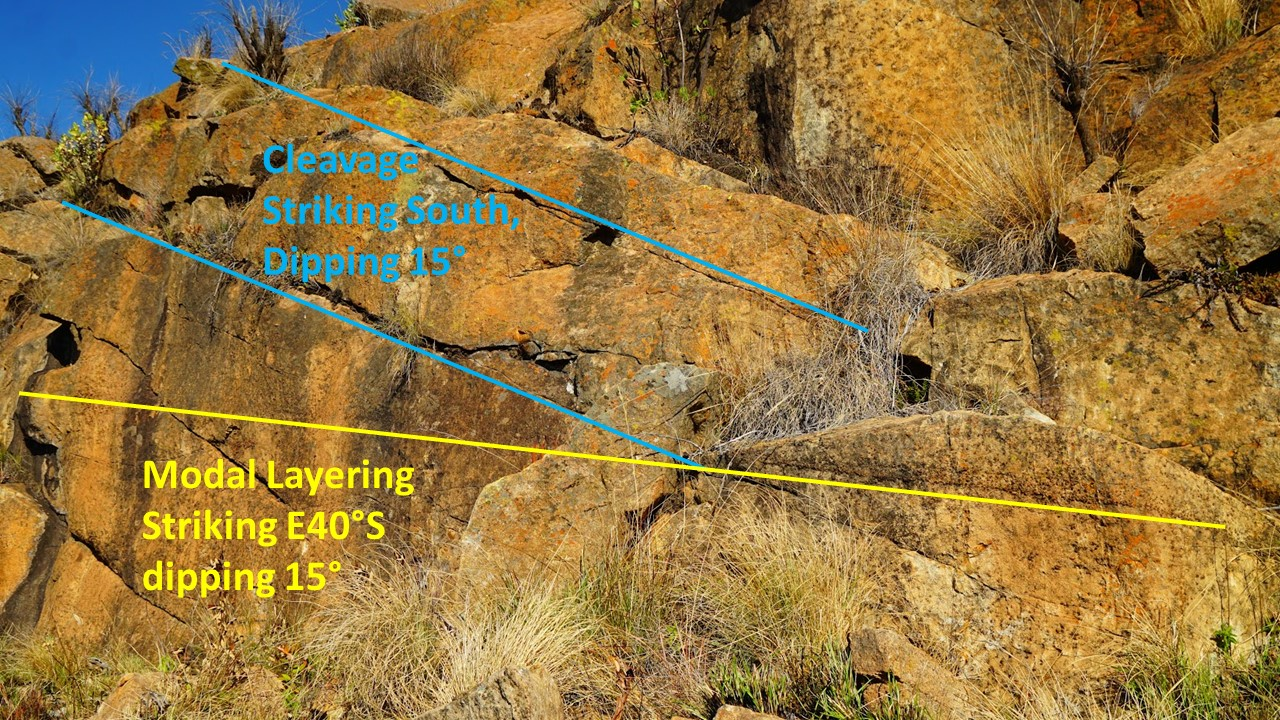
\includegraphics[width=\linewidth]{photo115_annotated_cleavage_modal_layering.jpg}
  \caption{Cleavage and modal layering forming distinct planes in a Mottled
    Anorthosite outcrop (annotated photo~\ChFivePhoto{115}).}
  \label{fig:ch5-ma-cleavage-photo}
\end{figure}

\subsection{Structural Observations}
\label{sec:ch5-structural-observations}

Structural measurements across the field area, together with the traced
lower Main Zone anorthosite marker beds, are mapped in
Figure~\ref{fig:ch5-structural-map}.

\afterpage{%
\begin{landscape}
\begin{figure}[p]
  \centering
  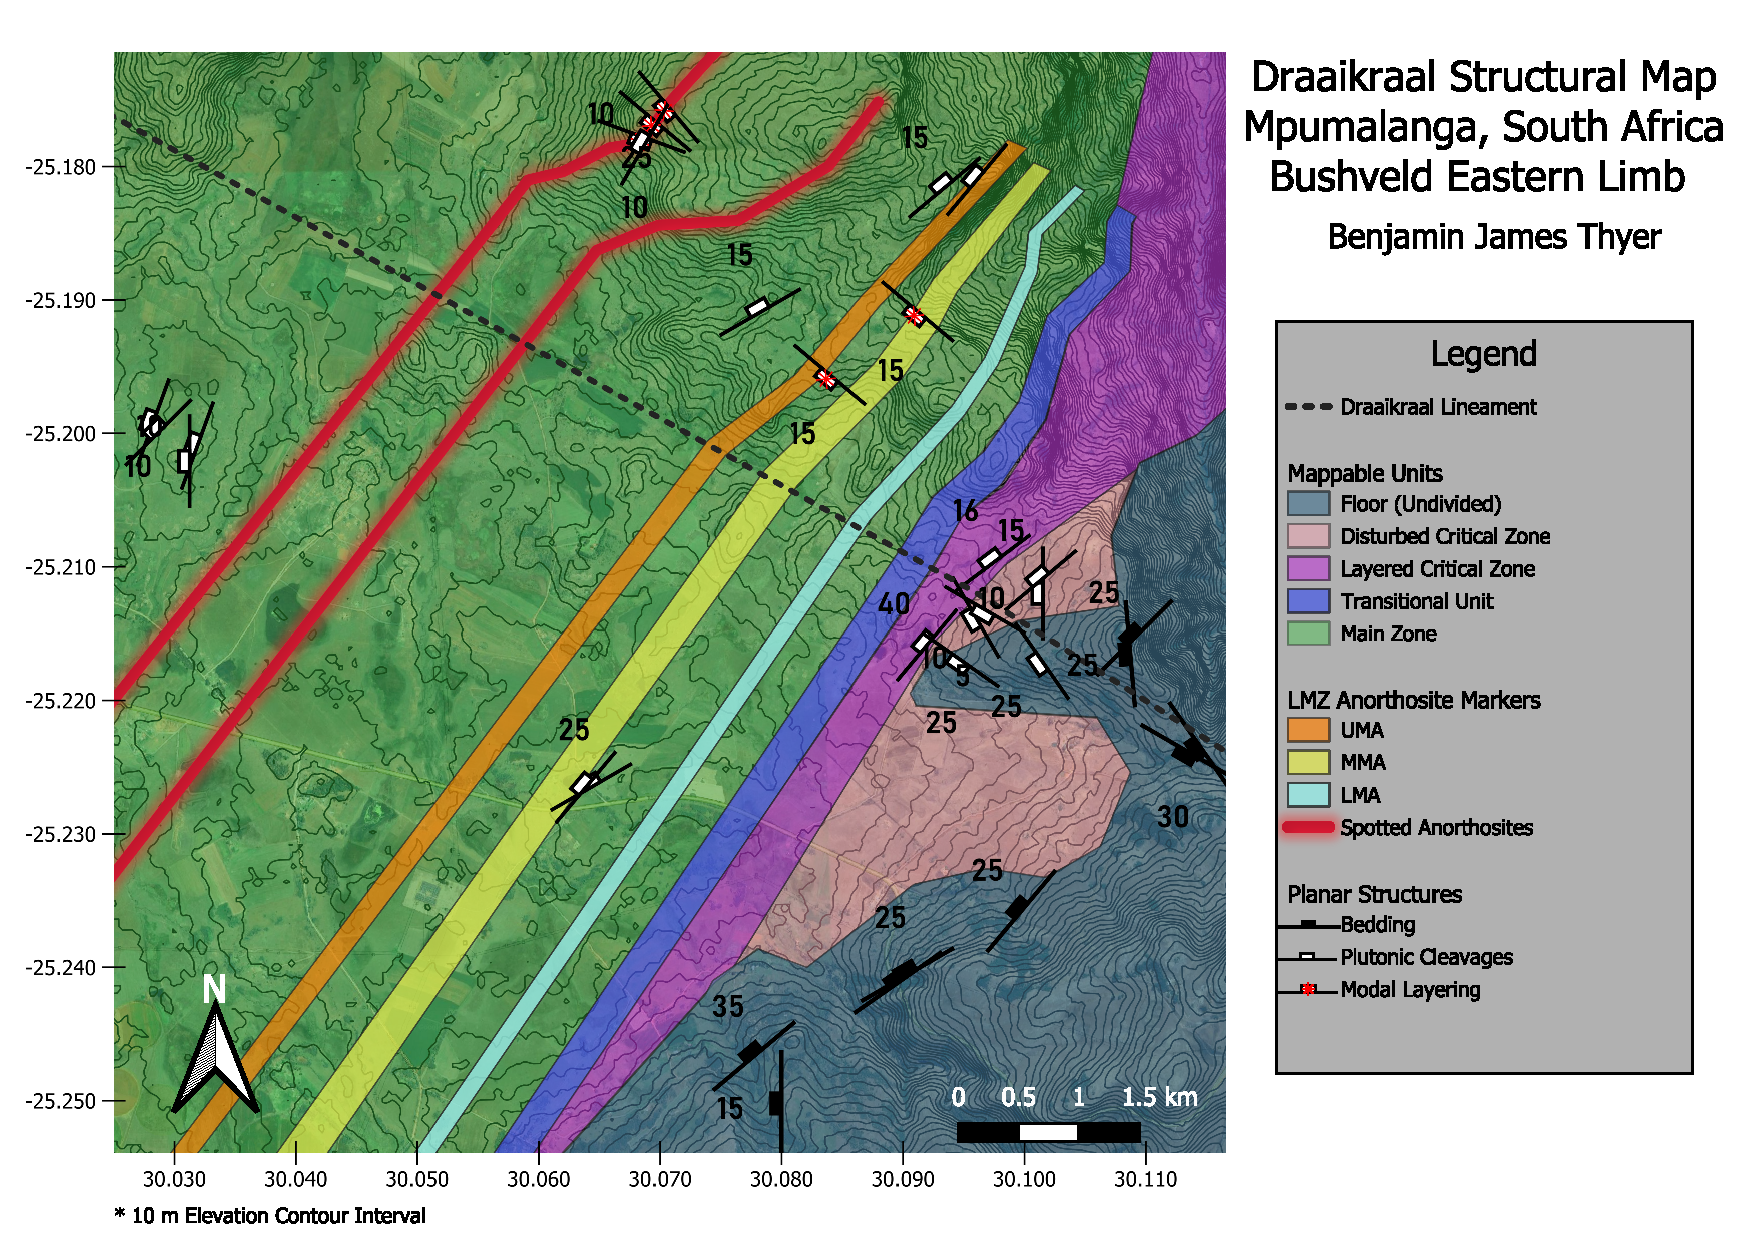
\includegraphics[width=\linewidth,height=0.8\textheight,keepaspectratio]{structural_map.pdf}
  \caption{Structural map of the Draaikraal field area: strike and dip of bedding,
    plutonic cleavage, and modal layering, over the mappable units (floor, Disturbed
    Critical Zone, Layered Critical Zone, Transitional Unit, Main Zone), with the lower
    Main Zone anorthosite marker beds (LMA, MMA, UMA, and the spotted anorthosites) and
    the Draaikraal Lineament (dashed). 10~m elevation contour interval. Measurements are
    listed in Table~\ref{tab:ch5-field-stations}.}
  \label{fig:ch5-structural-map}
\end{figure}
\end{landscape}}

\subsubsection{Kliprivier Synform}
\label{sec:ch5-kliprivier-synform}

\afterpage{%
\begin{landscape}
\begin{figure}[p]
  \centering
  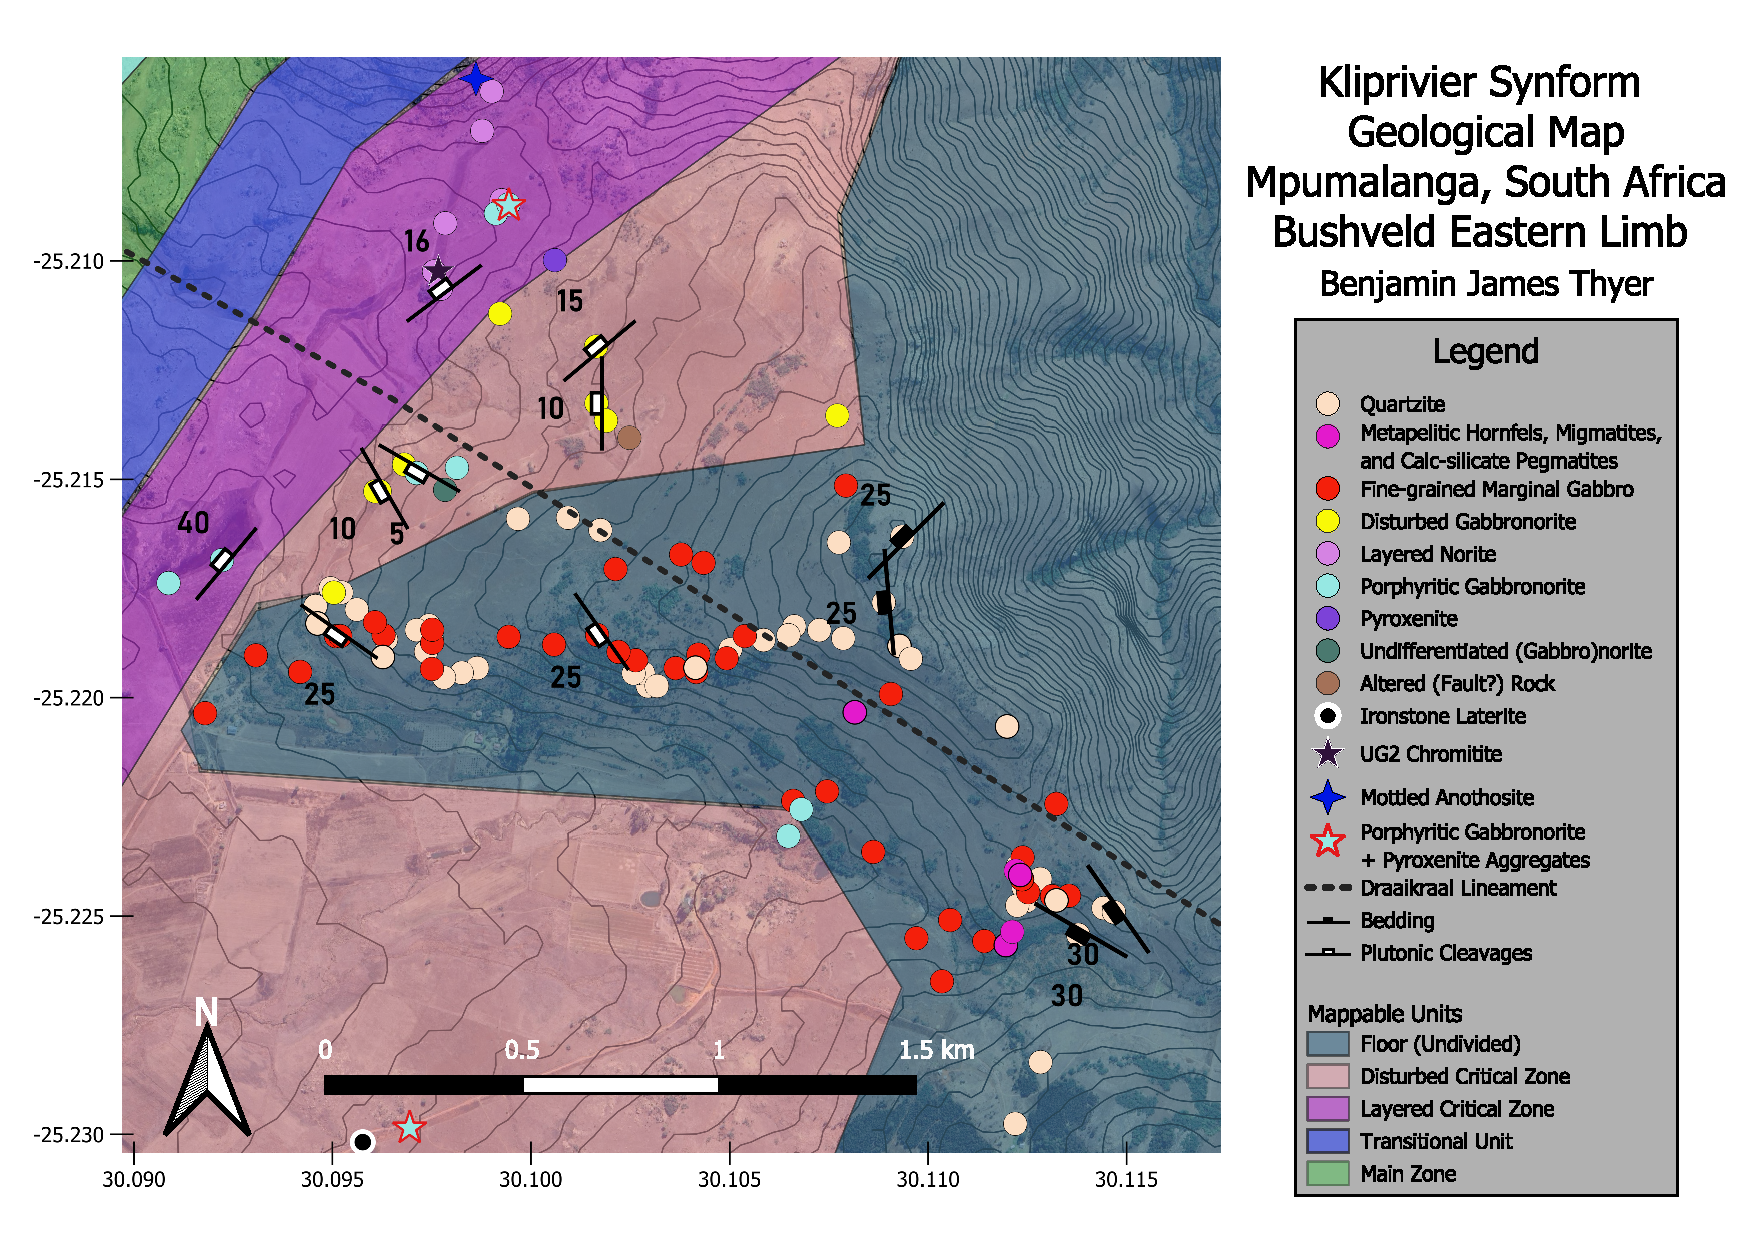
\includegraphics[width=\linewidth,height=0.8\textheight,keepaspectratio]{kliprivier_synform_map.pdf}
  \caption{Geological map of the Kliprivier Synform. Field observations are colored by
    lithology over the mappable units (floor, Disturbed Critical Zone, Layered Critical
    Zone, Transitional Unit, Main Zone), with bedding and plutonic-cleavage measurements
    and the Draaikraal Lineament (dashed).}
  \label{fig:ch5-kliprivier-map}
\end{figure}
\end{landscape}}

The most interesting large-scale structure in the mapping area
(Figure~\ref{fig:ch5-kliprivier-map}) is a
rotated package of disturbed, pegmatoidal upper Critical Zone
pyroxenites and gabbronorites {[}photos~\ChFivePhoto{61},\ChFivePhoto{62}, \ChFivePhoto{72}--\ChFivePhoto{78}{]}, well-cleaved
leuconorite layers {[}photo~\ChFivePhoto{63}{]}, quartzites {[}photos~\ChFivePhoto{28} and \ChFivePhoto{124}{]},
migmatized/hornfelsed argillites and calc-silicate layers {[}photos~\ChFivePhoto{29},
\ChFivePhoto{30}, and \ChFivePhoto{125}{]}, and marginal sills {[}photo~\ChFivePhoto{57}{]} in the northern
portion of Kliprivier Farm. The structure is remarkable because it
apparently displaces a marginal package of metasediments and
fine-grained sills over 1 km into the plutonic RLS. This
structure is described accurately but qualitatively by
\citet{vandermerwe2007}, who investigated the area to assess its platinum resource
potential. \citet{vandermerwe2007} refers to this feature the ``Kliprivier
Syncline'', though it is not clear if he is naming the structure or it
was named elsewhere. A displaced quartzite layer within the structure
was also observed during the field mapping of the Main Zone mottled
anorthosites by \citet{latypovetal2022} and is described in their
supplementary information as a ``Large Quartzite Xenolith?''.

The structure is referred to here instead as the ``Kliprivier Synform''
to recognize that it is not yet well understood. For instance, no
previous work to date has correlated marginal magmas and country rocks
from the two limbs of the putative syncline to demonstrate that they are
the same and that the structure is indeed a fold and not another
structure, such as a laccolithically deformed roof remnant of an RLS
subchamber or a package of floor rocks entrained in a rising magma. The
map presented here offers additional details that elucidate the nature
of this structure. Below, a series of observations of the Kliprivier
Synform is presented:

\begin{enumerate}
\def\labelenumi{\arabic{enumi}.}
\item
  To the north of the structure, there is a continuous, 90° gradual
  change in strike moving from finely-banded noritic Critical Zone,
  which strikes southwest and dips northwest like the majority of the
  mapped lithologies east of Draaikraal, to a southeastern strike
  dipping southwest. This gradual change in structure is accompanied by
  lithologic changes in the Critical Zone: Near and at the deformed
  areas, grain-size increases (photo~\ChFivePhoto{61}) and stratiform modal layering
  ceases and is replaced by a heterogeneous rock with abundant
  fine-grained Marginal Zone xenoliths, anorthosite autoliths (photo~\ChFivePhoto{62})
  and irregular clumps of pyroxene surrounded by anorthosite (photos~\ChFivePhoto{72}--\ChFivePhoto{77}). I have mapped these lithologies as ``Disturbed Gabbronorite''
  (Lithologic code: Dcg).
\item
  To the south, there is little exposure and no structural data could be
  gathered to pinpoint the reversal of the structure back to the common
  northwestern dip. However, outcrops constrain the contact between the
  Marginal Zone magmas and the porphyritic gabbronorite of the upper
  Critical Zone to occur within 10 meters. The ``disturbed'' lithologies
  of the Marginal/Critical zones present on the north side of the
  synform are not present on the south side. \citet{vandermerwe2007}
  interprets faulting with downthrows to the south at this contact;
  however, \citet{vandermerwe2007} does not map any vertical displacement of
  marker beds such as the UG2 chromitite at this fault.
\item
  Stratigraphically higher plutonic rocks are undeformed, suggesting
  that they were intruded and crystallized after the deformation forming
  the Kliprivier Synform. Interestingly, the western termination of the
  synform as mapped here occurs at or slightly below the level of the
  Merensky Reef, where a significant magma recharge event corresponding
  to the emplacement of the Main Zone is thought to have occurred
  \citep{seabrook2005,cameron1982}.
\item
  Displaced plutonic rocks to the north are stratigraphically below the
  quartzites and Marginal Zone sills, meaning that the section of sills
  and sediments serve as a roof to the RLS to the north.
\item
  Within this study, there is one strike and dip measurement immediately
  to the west of the structure, that is striking SW like the majority of
  the field area but is dipping more steeply than other rocks in the
  region. \citet{latypovetal2022} also report an unusually steeply dipping
  plutonic rock along strike.
\item
  To the east, the structure is attached to the floor of the RLS.
  Unfortunately, that area was not mapped in detail and the nature of
  the rotation from the synform's exotic dip to the common dip of the
  marginal series was not observed.
\end{enumerate}

   The calculated fold axis (Figure~\ref{fig:ch5-stereonets}b) trends roughly W5°N, plunging 15°, similarly to the
Draaikraal Lineament. The calculated obtuse bisector axial plane strikes W5°N and dips 85°.

The axial plane is similar in orientation to the WNW-ESE trending
Draaikraal Lineament that bounds the topographically high and low Main
Zone rocks. 

\begin{figure}[htbp]
  \centering
  \begin{subfigure}[t]{0.48\linewidth}
    \centering
    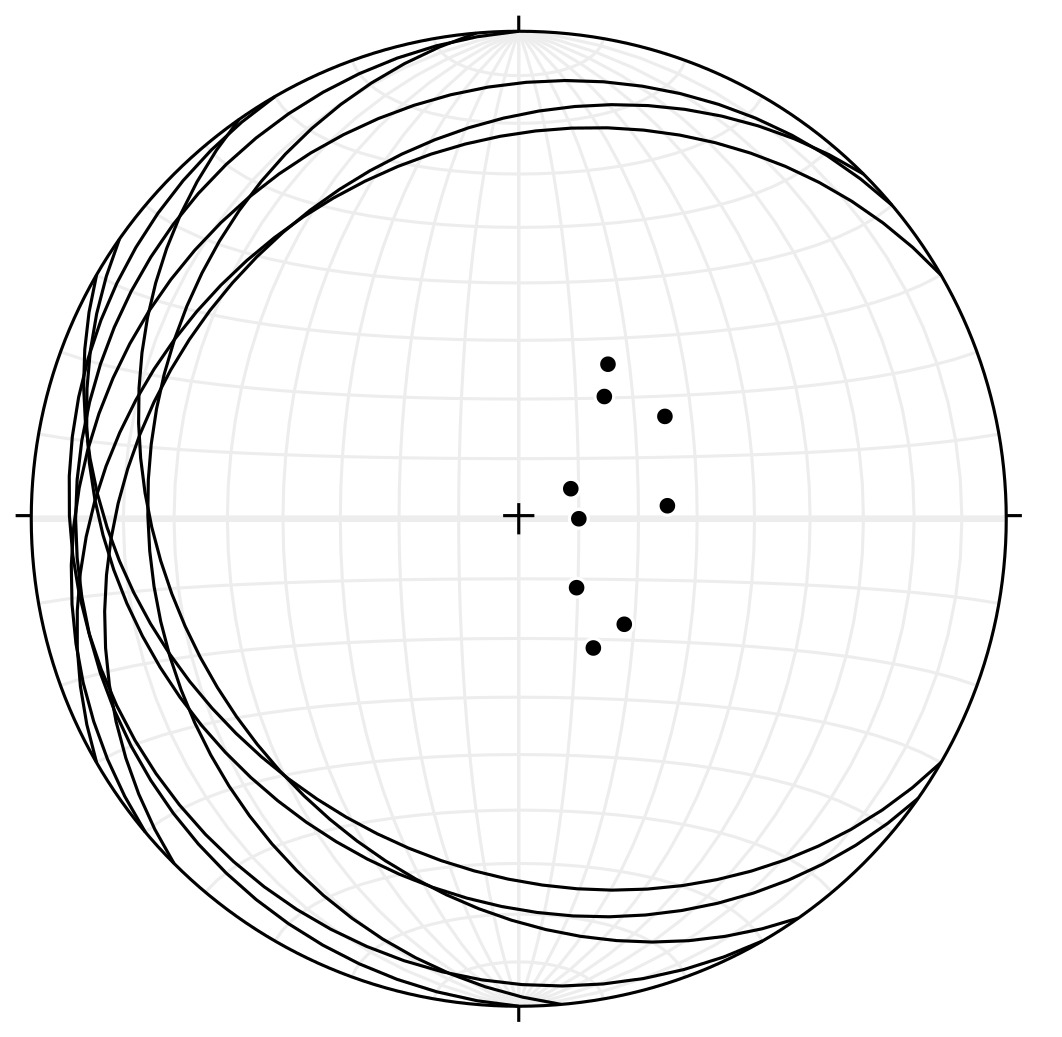
\includegraphics[width=\linewidth]{kliprivier_stereonet_bedding_poles.jpg}
    \caption{}
    \label{fig:ch5-stereonets-bedding}
  \end{subfigure}\hfill
  \begin{subfigure}[t]{0.48\linewidth}
    \centering
    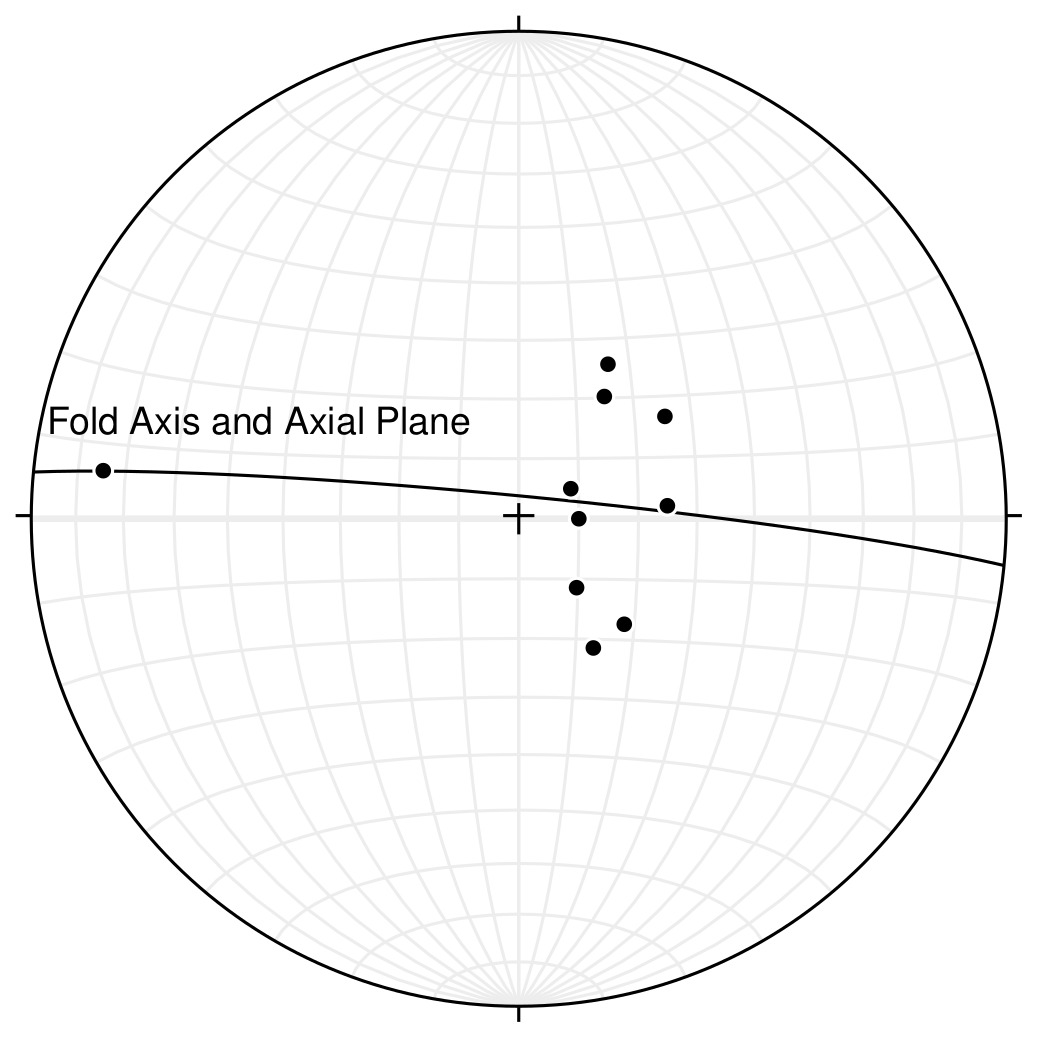
\includegraphics[width=\linewidth]{kliprivier_stereonet_fold_axis.jpg}
    \caption{}
    \label{fig:ch5-stereonets-fold-axis}
  \end{subfigure}
  \caption{Structural analysis of the Kliprivier Synform in stereographic projection
    (Stereonet 11; \citealp{allmendinger2012,cardozo2013}). (a) Bedding planes and poles
    to planes of rocks within the Kliprivier Synform. (b) Calculated fold axis and axial
    plane for the Kliprivier Synform.}
  \label{fig:ch5-stereonets}
\end{figure}

\section{Discussion}
\label{sec:ch5-discussion}

\subsection{Origin of the Kliprivier Synform and Draaikraal Lineament}
\label{sec:ch5-origin-of-the-kliprivier-monocline-and-draaikraal-lineament}

\citet{vandermerwe2007} described a ``synformal structure'' on Kliprivier
farm and referred to it as the ``Kliprivier Syncline'', but I identified
only a single, exotically-dipping limb within the structure with a
gradual southerly change in strike, therefore I interpret it here as a
monocline.

\citet{vandermerwe2007} brings attention to the PGE grade of such
structures along the eastern margin of the RLS, which often are rich in
sulfides and contain unusually high-grade Pt ores aside from the
traditional targets: the UG2 chromitite layer and the Merensky Reef 
(\S\ref{sec:ch5-the-origin-of-the-merensky-reef-and-pge-mineralization}, ``\nameref{sec:ch5-the-origin-of-the-merensky-reef-and-pge-mineralization}''). 
\citet{vandermerwe2007} believes that the Kliprivier structure and these other
sulfide traps predate Bushveld magmatism; however, I identified multiple
coarse-grained plutonic rocks of the upper Critical Zone that were rotated
within the structure. No Main Zone or Transition Zone rocks
exposed on the surface to the west of the Kliprivier are deformed within
the Kliprivier Synform, suggesting that deformation preceded the
crystallization of the Main Zone. This relative ordering requires that
the structure is synmagmatic. This interpretation is also supported by 
evidence for viscous deformation of gabbroic pegmatoids on the synform 
(Figure~\ref{fig:ch5-photo60-deformation}).

I interpret this
unit to be formed by synmagmatic deformation of nascent layered upper
Critical Zone mushes during the formation of the Kliprivier Synform,
effectively breaking up and redistributing the nascent layering into
many blobs.


% Photo 60 + digitized deformation-history sketches (2026-10-27). Schematic:
% Chapter5/Figures/fig_photo60_deformation.py -> generated/photo60_deformation_schematic.pdf
\begin{figure}[tbp]
  \centering
  \begin{subfigure}[t]{\linewidth}
    \centering
    \includegraphics[width=\linewidth]{Chapter5/Figures/generated/field_photos/DrBV60.jpg}
    \caption{}
    \label{fig:ch5-photo60-deformation-photo}
  \end{subfigure}\\[4pt]
  \begin{subfigure}[t]{\linewidth}
    \centering
    \includegraphics[width=\linewidth]{photo60_deformation_schematic.pdf}
    \caption{}
    \label{fig:ch5-photo60-deformation-schematic}
  \end{subfigure}
  \caption{(a) Sheared magnetite pegmatoid inclusion within non-magnetic marginal rocks,
    interpreted as reacted sediments, on
    the western side of the Kliprivier Synform (photo~\ChFivePhoto{60}). The
    pegmatoid is about 15~cm long. (b) Interpreted deformation history: 
    (1) mafic pegmatitic melt accumulates in lenses in
    migmatized sediment; (2) synmagmatic viscous deformation produces a sigmoid
    geometry; (3) post-magmatic brittle failure along an annealed fault truncates
    the lens and displaces its tip (lightly outlined). Black arrows show the sense
    of shear at each stage. The second stage of deformation may have occurred during isostatic flexure during cooling.
    The anneal of the fault suggests that it occurred at warm subsolidus conditions.}
  \label{fig:ch5-photo60-deformation}
\end{figure}

Structural analysis of the synform is consistent with gentle folding
along a fold axis plunging shallowly to the west with a subvertical
axial plane trending roughly E(SE)-W(NW) bisecting the limbs' obtuse
intersection angle (Figure~\ref{fig:ch5-stereonets}b). This deformation is subtle and would not
reverse the original ordering of the layered series and the marginal
series. A syncline alone cannot explain how the Marginal Zone of the
deformed, SW dipping limb came to be structurally higher than some of
the deformed plutonic rocks. It is, however, consistent with the idea
that much of the stratigraphically lower Critical Zone was intruded as
stacked sills from the north and terminated here, laccolithically deforming the overlying country rocks (\S\ref{sec:ch5-structure-and-relationship-to-country-rocks}). Within this paradigm, the
intruded Transvaal sediments ``displaced'' deeper within the RLS at the
Kliprivier Synform are actually roof rocks to the Critical Zone below
the level of the UG2. Given the intense melting and devolatilization of
the floor rocks in the area, it would not be surprising to find that the
thin strand of country rocks dividing the Critical Zone here beneath the
level of the UG2 would have been completely reacted to igneous minerals
and textures by reactive porous flow of magmas and hydrothermal fluids,
as has been argued for some Lower Zone and Marginal Zone rocks
\citep{yudovskaya2021}. Indeed, the ghosts of such transformed strands
may be expected at many locations throughout the complex and may have
separated sills of distinct composition or served as traps for
percolating melts or hydrothermal fluids. They may therefore be expected
especially at geochemical discontinuities within the stratigraphic
column, such as the Merensky Reef, Giant Mottled Anorthosite, Pyroxenite
Marker, Upper Mottled Anorthosite, etc.

\citet{sharpe1982} also reported that Critical Zone rocks but not
Main Zone rocks were deformed in the area, but attributed similar
small-scale folding on the margin to isostatic flexure. Isostatic
flexure has affected the modern expression of the Bushveld Complex
immensely, but a paleomagnetic study shows that isostatic flexure only
commenced within the Bushveld after cooling beneath the Curie
temperature of magnetite: 575°C \citep{hattingh1986}. This means that
flexure had to occur after termination of Bushveld magmatism and cannot explain synmagmatic
deformation. 

If the southwesterly dipping limb of the Kliprivier Synform is rotated
\textasciitilde20° about a level rotational axis trending
\textasciitilde45° NE to ``undo'' the local effects of postmagmatic
isostatic flexure that affected the RLS and its margin, the exotic limb
associated with the Kliprivier Synform would be dipping
\textasciitilde20° due south. This observation is consistent with the
hypothesis that an intrusion originating from the Thabazimbi-Murchison
Lineament to the north terminated in this area, producing a southerly
dipping monocline in its roof rocks.

The axial plane of the Kliprivier Synform is similar in orientation to the
Draaikraal Lineament (\S\ref{sec:ch5-kliprivier-synform}). Considering that the Kliprivier Synform also rests upon this
lineament, it is likely that the formation of the Kliprivier Synform is
related to the Draaikraal Lineament.

\subsection{Origin of Spheroidal Pyroxenite Aggregates (Tennis balls)}
\label{sec:ch5-origin-of-spheroidal-pyroxenite-aggregates-tennis-balls}

Spheroidal aggregates (SAs) of pyroxenite up to \textasciitilde5 cm are
known to occur as inclusions in the (gabbro)norites near the margin of
the RLS, and larger pyroxenite ``boulders'' within the Merensky Reef are
well-documented in the western limb of the RLS \citep{lee1979,smith2023,khoza2021}. The spherical agglomerates (also
called ``tennis balls'' due to their similar size) are richer in
pyroxenes, higher in An\# and pyroxene Mg\#, and richer in quartz and
sulfides than their (gabbro)noritic hosts \citep{lee1979,khoza2021}. Originally, dense groupings of these spherical aggregates were
thought to represent laterally continuous marker beds, but they cannot
be traced along strike of RLS layering for long distances relative to
the named reefs or mottled anorthosites-- instead they are most commonly
found \textless200m stratigraphically above the margin with the floor
rocks regardless of the stratigraphic position within the layered
series \citep{lee1979}. This author located isolated
pyroxenite tennisballs in porphyritic leuconorite in two places above
and below the Kliprivier Synform {[}photos~\ChFivePhoto{8}, \ChFivePhoto{79}{]}, on regions
previously mapped to contain tennisballs \citep{lee1979}. More
interestingly, this author located spheroidal aggregates of pyroxenite
in the fine-grained Marginal Zone {[}photos~\ChFivePhoto{2}, \ChFivePhoto{4}, \ChFivePhoto{96}{]}. Only very
recently have authors argued the marginal zone hosted spheroidal
aggregates at all. \citet{mitchell2023} used geochemical evidence
to claim the coarsely crystalline plutonic gabbronorites hosting the
Tennis Ball Marker (TBM), famously known on the Middelkraal farm, ought
to be considered as Marginal Zone and not as Main Zone as previously
mapped \citep{lee1979,molyneux2008,khoza2021}. Before
this work, no fine-grained marginal zone rocks had been reported to contain
pyroxenite tennis balls or spheroidal aggregates, although those
observed here in Draaikraal are much more lumpy and irregular than the
\emph{spheroidal} aggregates (SA) found in the Middelkraal TBM.

In photo~\ChFivePhoto{96}, the largest pyroxenite SA (\textasciitilde4 cm) resembles a
diapir: It has a long (\textasciitilde15 cm) and thin
(\textasciitilde\textless1 - 2 mm) pyroxenite tail developed behind it,
suggesting that it was migrating through a comparatively rigid,
stationary crystal-rich mush. The formation of a diapir suggests that
the SA was moving relative to the host rock and that the host rock was
more rigid than the pyroxenite. This requires explanation, as the
spheroidal aggregates contain more primitive pyroxenes and plagioclase
than the host matrix and are equilibrated at higher temperatures,
meaning that the pyroxenitic SAs would be more rigid than the host rocks
if one assumes the two are in thermal equilibrium.

There are three main hypotheses for formation of the spheroidal
pyroxenite aggregates in the RLS. The model of \citet{lee1979}
posits that pyroxenite aggregates are formed when a second, immiscible
fluid called the ``bridging'' liquid intrudes a magma body with
suspended pyroxene crystals. The bridging liquid preferentially ``wets''
the suspended pyroxene crystals, and entrains them as it coagulates with
other smaller, individual bubbles of the immiscible fluid entraining the
suspended pyroxenes of the host magma.

The second model of \citet{khoza2021} posits that a magma recharge event
introduces magma into a pyroxenite cumulus pile, breaking the pile into
pieces that are then subsequently entrained into the secondary magma.
This magma does not equilibrate with the pyroxenite; instead, it evenly
melts the rough edges of the pyroxenite aggregates, fashioning them into
spheres.

The third model posits that a pyroxenitic liquid or mush intrudes a
cooler crystal mush and is disaggregated into pyroxenite aggregates,
analogously to the formation of mafic enclaves in felsic plutons from
the disaggregation of intruded basalts \citep{mitchell2023,smith2023}. This is the model most compatible with the observation of
diapirism of spherical aggregates in the fine-grained marginal sill
phase, since it allows for the SAs to be formed by disaggregation of a
comparatively hot ultramafic magma intruded into comparatively cool (and
therefore rigid) mafic sills.

The diapiric movement of the pyroxenite spheroid in photo~\ChFivePhoto{96} serves as
good evidence against the second model of \citet{khoza2021}, as Khoza's model
requires the pyroxenite spheroids to be more rigid than the host magma,
so that they remain consolidated against the flowing host magma. If the
spheroidal aggregate was more rigid than the host magma, then it would
not have left a pyroxenitic tail behind it. Finally, if magma recharge
introduced into a pyroxenite cumulate pile forms SAs, then one would
expect them to be a ubiquitous feature throughout the Bushveld Complex
regardless of the distance from the margin, as the conventional and most
accepted model for the assembly of the Bushveld Complex evokes many
instances of magma recharge atop a preexisting cumulate pile \citep{holness2017,cawthorn2015}.

The model of \citet{lee1979} is interesting because secondary fluid
input both can explain the relative softness of the primitive SA
migrating through more evolved host rocks, and because it explains the
abundant quartz (\textgreater10\%: \citealp{lee1979}) in the
pyroxenite SA, which would not be expected for an ultramafic magma with
high Mg\# and An\#. Photos~\ChFivePhoto{97} and \ChFivePhoto{98} exhibit the migration of a distinct
secondary comagmatic silica-rich fluid through the marginal zone magmas.
However, \citet{mitchell2023} point out that multiple distinct
SA-rich horizons of the TBM exist but those that they report were over
100 meters from the alleged source of the fluids: the Dullstroom lavas
at floor of the magma chamber. Their model simply requires injection of
hot pyroxenite lavas into cooler mafic mushes. This author, however,
suggests that the secondary bridging liquids of Lee and Sharpe's model
could have percolated through homogeneous (gabbro)norites until
ultimately meeting a coarse, pyroxenitic horizon susceptible to
differential wetting.

The model of \citet{lee1979} offers a satisfactory explanation for
the SA's ties to the intrusion's margin. The secondary fluids that
circulated throughout the Bushveld chamber were predominantly sourced
from devolatilized and variably melted country rocks \citep[see also \S\ref{sec:ch5-stable-isotopes-of-the-rls}, ``\nameref{sec:ch5-stable-isotopes-of-the-rls}'']{schiffries1990,buick2000}, so Bushveld magmas near the margin would
be the most likely to encounter poorly mixed, newly-introduced
immiscible (or poorly miscible) fluids than magmas further from the
margin. The model of \citet{mitchell2023} also offers a plausible
explanation for the SAs' ties to the intrusion's margin, as the margin
would cool faster to create a larger temperature (and viscosity)
contrast between new pulses of pyroxenitic magmas and their host rocks.

\subsection{Correlation of the Mottled Anorthosites in the Lower Main Zone}
\label{sec:ch5-correlation-of-the-mottled-anorthosites-in-the-lower-main-zo}

Although there are three main named mottled anorthosite packages within
the lower Main Zone, there are also many other minor anorthosites
throughout the Main Zone \citep{sacs1980,vongruenewaldt1985}.
There is agreement between \citet{vandermerwe2007}, \citet{setera2018},
and \citet{latypovetal2022} about the location of the UMA on the
Roossenekal-Lydenburg road. I allow this agreement to calibrate the
naming of the area's mottled anorthosites. Additionally, \citet{vandermerwe2007}
and \citet{latypovetal2022} also mapped the MMA and LMA along the
Roossenekal-Lydenburg road at the same location as I have.

\citet{vandermerwe2007} maps the surface exposure of the UMA, MMA, and LMA
throughout the southern sector of the eastern limb of the RLS, and later
worked with \citet{latypovetal2022}, who undertook 6 stratigraphic
traverses throughout the southeast RLS to prove that these 3 marker beds
are laterally extensive throughout the entire Main Zone and do not abut
the country rocks, arguing that these continuous mottled anorthosite
packages were emplaced at the floor of an entirely molten 5 km thick
magma chamber. Three of these traverses overlapped with the field area
of this work. Within the field area, the UMA and MMA mapped by
\citet{vandermerwe2007} and \citet{latypovetal2022} are discordant; they do not
follow the regional dip to the northwest. I did locate anorthosites at
the coordinates provided in the SI by \citet{latypovetal2022}; however, I
conclude that the UMA and MMA that they have mapped in their traverse I,
north of the Draaikraal Lineament, are not the same anorthosites as
their mapped UMA and MMA south of the Draaikraal Lineament on the
Roossenekal-Lydenburg road in their traverse III. I further argue that
what they have mapped as UMA and MMA north of the Draaikraal Lineament
are actually spotted anorthosites and some lack mottles entirely.

Two claims should be distinguished here. The first, which I hold with
confidence, is that the anorthosites correlated with the UMA and MMA north
of the lineament by \citet{vandermerwe2007} and \citet{latypovetal2022} are
spotted anorthosites: they are thin, non-magnetic, and lack the coarse
oikocrystic mottles and associated pyroxenites that define the mottled
anorthosites of the lower Main Zone (Table~\ref{tab:ch5-ma-correlation}). The
second, which is tentative, is which of the northern mottled-anorthosite
packages corresponds to the UMA and which to the MMA.

Though this particular contested
correlation by \citet{latypovetal2022} is of minor significance to the
overall argument put forward in their work, it is essential evidence to
understand the origin and significance of the Draaikraal Lineament as
the surface expression of a synmagmatic monocline formed by laccolithic
deformation during the intrusion of much of the Critical Zone (see the end of this subsection).

The outcrops behind both correlations are compared in Table~\ref{tab:ch5-ma-correlation}; their photographs are in Appendix~\ref{app:draaikraal-field-data}.

% =============================================================
%  chapter5_ma_correlation.tex -- comparison of the lower Main Zone mottled
%  anorthosite correlations across the Draaikraal Lineament (Table). \input{} by Chapter5/Writing/chapter5_body.tex in the Discussion
%  (Correlation of the Mottled Anorthosites in the Lower Main Zone).
%
%  2026-10-29: the six-photo mosaic that followed the table was removed;
%  photos 49, 86, 87, 90 and 109 are back in the Appendix A album (with their
%  album captions), and photo 115 links to its annotated figure
%  (fig:ch5-ma-cleavage-photo).
% =============================================================

\begin{table}[tbp]
  \centering
  \footnotesize
  \setlength{\tabcolsep}{3pt}
  \caption{Lower Main Zone anorthosite outcrops compared across the Draaikraal
    Lineament. The roadcut of the UMA South of the lineament in particular is well documented and agreed to be a lower 
    Main Zone mottled anorthosite \citep{setera2018,latypovetal2022}. The
    outcrops north of the lineament as correlated by \citet{latypovetal2022} and \citet{vandermerwe2007} are compared with those in this work.
    Heights are stratigraphic heights above the Merensky Reef
    (\S\ref{sec:ch5-stratigraphic-column-methods}).}
  \label{tab:ch5-ma-correlation}
  \begin{tabular}{@{}>{\raggedright\arraybackslash}p{3.2cm}
                  >{\raggedright\arraybackslash}p{1.3cm}
                  >{\raggedright\arraybackslash}p{1.3cm}
                  >{\raggedright\arraybackslash}p{1.3cm}
                  >{\raggedright\arraybackslash}p{0.9cm}
                  >{\raggedright\arraybackslash}p{4.6cm}@{}}
    \toprule
    Outcrop & Photos & Height (m) & Thick. & Mag. & Texture and associated lithologies \\
    \midrule
    \multicolumn{6}{@{}l}{\textit{Upper Mottled Anorthosite (UMA)}}\\
    \addlinespace[2pt]
    Roadcut UMA, South
    \newline{\scriptsize $-$25.2274, 30.05494}
      & \ChFivePhoto{49}, \ChFivePhoto{53}, \ChFivePhoto{54}
      & 564 m & $\sim$0.5~m & yes
      & Anorthosite with $\sim$2cm oikocrystic pyroxene mottles overlying $\sim$0.5~m coarse feldspathic pyroxenite
        with anorthositic blocks, over fine-grained green gabbronorite with $\sim$ 1cm blebby bottle-green
        CPX; irregular, non-planar contacts \\
    \addlinespace[6pt]
    ``UMA'' of \citet{latypovetal2022}, North
    \newline{\scriptsize $-$25.1767, 30.07222}
      & \ChFivePhoto{86}
      & 1030 m & $\sim$10~cm & no
      & Anorthosite with $<$1~cm equant pyroxenes. No other unusual lithologies observed. Planar, concordant contacts \\
    \addlinespace[6pt]
    ``UMA'' of this work, ``LMA'' of \citet{latypovetal2022}, North
    \newline{\scriptsize $-$25.1821, 30.09749}
      & \ChFivePhoto{90}
      & 398 m & >10~cm & yes
      &  Anorthosite with coarse oikocrystic pyroxene mottles over coarse pyroxenite \\
    \midrule
    \multicolumn{6}{@{}l}{\textit{Middle Mottled Anorthosite (MMA)}}\\
    \addlinespace[2pt]
    Valley outcrop MMA, South
    \newline{\scriptsize $-$25.227, 30.06419}
      & \ChFivePhoto{103}--\ChFivePhoto{109}
      & 373 m & > 2 m & yes
      & Very thick; layers of oikocrystic mottled anorthosite and pyroxenite
        with both planar and wavy, discordant contacts \\
    \addlinespace[6pt]
    ``MMA'' of \citet{latypovetal2022}, North
    \newline{\scriptsize $-$25.1827, 30.08279}
      & \ChFivePhoto{87}
      & 708 m & not measured & no
      & Anorthosite with pyroxene spots and foliated (sheared) pyroxenes, no pyroxenites. \\
    \addlinespace[6pt]
    ``MMA'' of this work, North
    \newline{\scriptsize \todo{coordinates}}
      & \ChFivePhoto{115}
      & 333 m & > 4 m  & yes
      & Thick package of anorthosites with coarse oikocrystic pyroxene mottles and pyroxenites with sharp lower contacts
      that grade upward to anorthosite in $\sim$ 20 cm layers; cleavage discordant with modal layering \\
    \bottomrule
  \end{tabular}
\end{table}



The UMA outcrop on the Roossenekal-Lydenburg road (photos~\ChFivePhoto{53}, \ChFivePhoto{54})
contains a distinct package of a striking magnetic mottled anorthosite,
\textasciitilde0.5m thick underlain by a \textasciitilde0.5m
coarse-grained feldspathic pyroxenite with some reacted anorthositic
blocks and pure anorthosite bands. This pyroxenite is in turn underlain
by a unique rock interpreted to be a fine-grained gabbronorite
containing blebby anhedral bottle-green clinopyroxene phenocrysts. Fresh
faces of this rock are a uniquely vivid green color. I was able to
locate the vivid green fine grained gabbronorite with blebby anhedral
pyroxene phenocrysts (Fgog) above the Draaikraal Lineament near a cliff
with a view of the Booysendal PGE mine to the east (Fgog not pictured,
photos~\ChFivePhoto{88} and \ChFivePhoto{90}). I correlate this outcrop with the UMA south of the Draaikraal Lineament
because it preserves the same sequence of fine-grained green gabbronorite,
coarse feldspathic pyroxenite and magnetic mottled anorthosite. It sits
\textasciitilde170~m lower in the stratigraphic column (398~m versus 564~m
above the Merensky Reef; Table~\ref{tab:ch5-ma-correlation}). The match is not
perfect, but the column assumes a constant strike and dip
(\S\ref{sec:ch5-stratigraphic-column-methods}). Over the \textasciitilde6.5~km
separating the two outcrops along strike, small discrepancies between the
modeled and true strike and dip could produce significant variation in the
stratigraphic heights.

It is possible that this northern package is instead the MMA. That would
imply that the fine-grained green gabbronorite is not unique to the UMA but
also occurs beneath the MMA. It would not change the argument below: either
way, the northern correlatives are magnetic mottled anorthosites with
associated pyroxenites, and they lie at heights close to those of the
southern packages.

The anorthosite mapped by \citet{vandermerwe2007} and \citet{latypovetal2022}
as the UMA north of the Draaikraal Lineament (photo~\ChFivePhoto{86}) is very small
(\textasciitilde10 cm), non-magnetic, and lacks the associated
coarse pyroxenite and fine-green gabbronorite lithologies; it does not
resemble the UMA outcrop on the Roossenekal-Lydenburg road. Furthermore,
it is significantly stratigraphically higher: \textasciitilde1030~m above the Merensky Reef. \citet{vandermerwe2007} does not report
displacement of the UG2 over the Draaikraal Lineament, so it is
interesting that their UMA is given \textasciitilde470~m of stratigraphic displacement.

Similarly, the discordant MMA correlation they offer does not stand up.
The MMA is supposed to be a striking and very large marker in the lower
Main Zone (photos~\ChFivePhoto{103}--\ChFivePhoto{109}), and yet the outcrop they correlate (photo~\ChFivePhoto{87}) is a small exposure with subtle, non-magnetic pyroxene
spots/mottles, and no associated blebby or coarsely layered pyroxenites.
I instead find the concordant correlation of a very large package of
magnetic mottled anorthosites with coarsely layered pyroxenites at photo~\ChFivePhoto{115} much more plausible.

Neither correlation places the anorthosites at exactly the same height on
both sides of the lineament, and neither needs to. The thickness of the
anorthosite packages and of the layers between them may vary along strike,
shifting their relative positions coherently even without invoking a fault.
Nonetheless, I prefer the simplest explanation that explains the data. My
correlation follows petrography, and happens to require the smallest lateral
change to explain the observations: the mottled anorthosites can be followed
across the Draaikraal Lineament without invoking a fault.

Because there are essentially no detailed studies of the lower Main Zone
anorthosites \citep[similar to][for the GMA of the
transitional unit]{mitchell2002}, it is easy to fall prey to one's confirmation bias:
one can find an anorthosite in the lower Main Zone without too much
trouble. Detailed and careful petrography of these marker beds is
necessary to make correct correlations. The strategy of
\citet{latypovetal2022} to use these marker beds to understand the structure and
petrogenesis of the RLS is excellent; however, I would argue instead
that one should first focus on one particularly remarkable anorthosite
package (perhaps the MMA or UMA), and should follow it along strike. For
this field area, I would want to do a detailed characterization of the
Transitional unit, LMA, MMA, and UMA stratigraphy to the north of the
Draaikraal Lineament to get complete sections of the remarkable, but
incomplete, outcrops exposed along the Roossenekal-Lydenburg road. Then
I would follow the anorthosites up north to examine how their strike
might change, as their regionally concordant NW dip would quickly become
discordant to the north. I consider the following open questions to
remain:

1) Are the LMA, MMA, and UMA generally planar features, irregular
contacts aside?

2) For how long are they laterally continuous?

3) Where and why are they discordant to the regional layering, if ever?

4) Do they abut the floor?

5) How do the distances between them vary at different locations within
the intrusion?

\subsection{Origin of the Mottled Anorthosites in the Lower Main Zone}
\label{sec:ch5-origin-of-the-mottled-anorthosites-in-the-lower-main-zone}

Surprisingly little attention has been given to the spectacular
anorthositic sequences of the lower Main Zone. More often, anorthosites
from the Critical (or Transitional) Zone are studied \citep{mitchell2002,maier2016,mitchell2019,maier2020,barnes2021}, or at the top of the Main Zone at the
Pyroxenite Marker \citep{bourdeau2021,bourdeau2023}. The Upper Mottled
Anorthosite (UMA) and Pyroxenite Marker of the Main Zone are known to
demarcate significant geochemical and isotopic changes in the RLS
stratigraphy \citep{klemm1985,kruger1994,vantongeren2013}, most often ascribed to magma recharge (\S\ref{sec:ch5-radiogenic-isotope-stratigraphy-of-the-rls}, ``\nameref{sec:ch5-radiogenic-isotope-stratigraphy-of-the-rls}'').

In the East and West Limbs, the mottles of the lower Main Zone mottled
anorthosites (LMA, MMA, UMA) are surprisingly iron-rich-- the pyroxenes
have much lower Mg\# than the surrounding gabbronorites \citep{scoonmitchell1994,mitchelleales1998}. Though I was surprised to find
the mottles of these three units were magnetic at first, it had already
been known that they produce subtle but distinct magnetic anomalies
observable in aerial surveys, at least within the West Limb \citep{viljoen1985,cole2013}. \citet{viljoen1985} point out that
the stratigraphic magnetic anomalies of the mottled anorthosites of the
lower Main Zone are not present near structural weaknesses, like faults.

\citet{scoonmitchell1994} make the provocative argument that the
silicate iron-rich ultramafic pegmatites (IRUPs) of the upper Critical
and lower Main Zones are sourced from accumulated evolved fluids
interstitial to these mottled anorthosites of the lower Main Zone. These
putative residual melts are argued to flow laterally, eventually
exploiting structural weaknesses to percolate downward to replace
plagioclase-rich, magnesian cumulates with olivine-pyroxene Iron-Rich
Ultramafic Pegmatites (IRUP), a lithology where plagioclase is
conspicuously absent. This bold argument seems unnecessary. It is easy
to explain, as \citet{scoonmitchell1994} also do, that IRUPs likely
originated from downward-percolating immiscible Fe-oxide melts from the
Upper Zone. Strontium isotopes within IRUPs are uniform regardless of
stratigraphic height and are identical to the Upper Zone \citep{scoonmitchell1994}. IRUPs are known to occupy any location along the
stratigraphic column between the Upper Zone and their lowest occurrences
in the upper Critical Zone, and form a geochemical continuum that
records them becoming more magnesian and silica-rich with depth,
transitioning from Fe-Ti oxide pegmatites to Fe-rich silicate
pegmatites, telling a clear story of evolution/hybridization of
downward-percolating, dense Fe-rich liquids.

Still, the strontium isotopes of these mottled anorthosites and some
stratigraphically proximal gabbronorites are often discontinuous with
the otherwise homogeneous, isotopically evolved Main Zone immediately
surrounding them, and instead are, remarkably, identical to the Upper
Zone and IRUPs \citep{karykowski2017,kruger1994}. It may very well
be true that the IRUPs are related to the mottled anorthosites of the
lower Main Zone, though I would instead propose that these anorthosites
might have served as porous ``aquifers'' that trapped IRUP melts
originating from the Upper Zone, rather than pose the mottled
anorthosites as the source of these iron-rich melts.

Additionally, compelling geochemical arguments have been presented on
texturally similar mottled anorthosites in the Critical Zone that argue
for formation by reactive porous flow of a hydrothermal fluid including
the presence of evolved but Ni--rich olivine, hydrous phases and
sulfides, and extreme reverse zoning of plagioclase surrounding mottles \citep[see also \S\ref{sec:ch5-origin-of-enigmatic-monomineralic-igneous-rocks}, ``\nameref{sec:ch5-origin-of-enigmatic-monomineralic-igneous-rocks}'']{maier2020}. The presence of water is known to favor olivine
crystallization at the expense of pyroxenes, as well as favoring more
anorthitic plagioclase over albite \citep{baker2019}.

I envisage mottled, stratiform anorthosites to form where
low-permeability structural traps collect upward-percolating reactive
hydrothermal fluid that locally favors plagioclase crystallization and
pyroxene dissolution. EPMA work on the mottles of the LMA, MMA, and UMA
would bring clarity to the relative importance of evolved interstitial
fluids, potential IRUP contaminants, and hydrothermal fluids on the
formation of mottled anorthosites in the lower Main Zone and to
stratiform anorthosites in general.

\subsection{Rethinking the Marginal Zone: Arguments for Incremental Assembly}
\label{sec:ch5-marginal-zone-rethink}

The Marginal Zone has been traditionally understood to be the chilled
margin of the RLS \citep{harmer1985}. However, detailed work
reveals that the lowest stratigraphy of the RLS is complex. The Marginal
Zone is not always present at the floor of the RLS, especially to the
southeast \citep{molyneux2008,vandermerwe2007,latypov2020}.
Marginal Zone norites may locally intrude the Lower Zone \citep{wilson2017,yudovskaya2021}, and the Marginal Zone overlies an
additional Bushveld-related ultramafic sequence referred to as the
Apiesdooringdrai peridotite body or Basal Ultramafic Sequence (BUS) at
Burgersfort that is more likely to contain chilled components of the
earliest RLS-related intrusions \citep{wilson2012,wilson2017}. The
BUS, Marginal Zone, and Lower Zone all contain reacted sedimentary
``rafts'' or xenoliths with igneous mineralogy \citep{yudovskaya2021}.
Thinner ultramafic and mafic sills likely related to Bushveld
magmatism intrude the floor rocks kilometers below the mapped Marginal
Zone \citep{sharpehulbert1985}. In my field work, I observed that
Marginal Zone sills seemed to concordantly intrude the Transvaal
sediments below the RLS for many kilometers.

The lack of a cohesive igneous stratigraphy and the geochemical and
isotopic variability of the Marginal and Lower Zones led
\citet{mitchell2023} and \citet{scoon2023} to propose that the Marginal
and Lower Zones were assembled incrementally by magmas of different compositions (see also \S\ref{sec:ch5-magma-chamber-scales}, ``\nameref{sec:ch5-magma-chamber-scales}''). I would extend their arguments to the entire RLS. I posit
that a series of stacked peridotites, pyroxenites, norites,
gabbronorites, and gabbros were emplaced, somewhat self-sorted according
to density and the compositional control on stalling depth (more
primitive magmas will crystallize at higher temperatures) at the
location of the BUS, RLS and Marginal Zones presently. I suggest that
postcumulus modification by reactive porous flow of late stage magmas
and/or hydrothermal fluids allowed for dissolution and recrystallization
to produce phaneritic textures within the RLS, and that these fluids
interacted with the Marginal Zone to a far lesser extent than the
greater RLS. These fluids reequilibrated and reacted with the RLS within
a depth-controlled thermal gradient which produced the RLS-scale
cohesive geochemical trends that are mostly uncorrelated with isotopic
and lithological boundaries \citep[see][]{eales1986}. Subconcordant
intrusion of magmas as sills into the country rock results in the
inclusion of abundant but comparatively volumetrically small strands of
sedimentary rock in the Lower, Marginal, Critical, and Main Zones of the
RLS. These strands react to igneous mineralogy by reactive porous flow
along grain boundaries and develop planar modal layering due to lateral
transit of fluids and evolved magmas sourced from the
Thabazimbi-Murchison Lineament (TML) and they serve as traps for
hydrothermal fluids that locally supported the reaction, dissolution,
and crystallization of mafic lithologies into mottled anorthosites
below. The Merensky Reef represents a structural trap for a reduced
supercritical carbon-based fluid \citep[see also \S\ref{sec:ch5-unusual-volatile-phases-in-the-lower-rls}, ``\nameref{sec:ch5-unusual-volatile-phases-in-the-lower-rls}'']{ballhaus1985}. The
isotopic homogeneity of the Upper Zone (\S\ref{sec:ch5-open-or-closed-system}, ``\nameref{sec:ch5-open-or-closed-system}'') allows for a more orthomagmatic
interpretation: perhaps it represents a magma chamber where evolved
tholeiitic magmas and hydrothermal fluids collected, and
magnetite/anorthosite layers were crystallized by cycles of
depressurization, cooling, and perhaps magma recharge.

\subsection{Significance of Rock Cleavage and Modal Layering Orientation in the RLS}
\label{sec:ch5-cleavage-significance}

The discordance of rock cleavage and modal layering (\S\ref{sec:ch5-cleavage-layering}; Figure~\ref{fig:ch5-ma-cleavage-photo}) suggests that cleavage and modal
layering are formed by distinct processes that may have occurred at
different times, with modal layering likely predating the formation of
rock-cleavage.



There may have been multiple processes generating superimposed fabrics
in the plutonic RLS. For instance, rock fabrics may have been developed
in two phases, perhaps a primary fabric (modal layering) developed by
gravity and crystal settling (\S\ref{sec:ch5-layered-mafic-intrusions}), then a second by lateral flow of
hydrothermal fluids, or by differential contractions during cooling.
Care must be taken when interpreting planar measurements in plutonic
rocks of the RLS. The bimodal planes of the RLS in this field area may
be due to an initial development of south-dipping igneous fabric above
the Kliprivier Synform as magmas filled a local basin towards the
south before another generation of paleohorizontal fabric developed
perpendicular to thermal gradients due to differential contraction
during cooling.

\section{Conclusions}
\label{sec:ch5-conclusions}

\begin{enumerate}
\def\labelenumi{\arabic{enumi})}
\item
  The field data of this study support the interpretation that the
  Kliprivier Synform is a monocline synmagmatic with the Critical Zone
  below UG2, predating the UCZ at UG2 and up. There is no displacement
  of marker beds above UG2, including all mottled anorthosites. The
  country rocks and Marginal Zone sills of the Kliprivier Synform are
  roof rocks to the Critical Zone below UG2 and are the floor to
  undeformed Transitional and Main Zone.
\item
  The Draaikraal Lineament is best explained as the surface projection
  of the subvertical axial plane of the Kliprivier Synform. It is
  hypothesized that trapped fluids from the emplacement of the
  underlying Critical Zone may have exploited the deformed Kliprivier
  Synform, developing a vertical, planar fluid conduit at the
  Draaikraal Lineament where upwardly migrating fluids may have escaped,
  developing recessive lithologies. The regional recessive topography of
  the Main Zone south of the Draaikraal Lineament is proposed to
  originate from relatively high degrees of contamination from
  devolatilized/melted underlying sediments relative to the Main Zone
  lithologies at the same stratigraphic height to the north of the
  Draaikraal Lineament.
\item
  The discordant mottled anorthosite correlation above and below the
  Draaikraal Lineament by \citet{vandermerwe2007} and \citet{latypovetal2022}
  is locally incorrect. The field work presented here instead suggests
  that the mottled anorthosite marker beds of the lower Main Zone are
  concordant and undisplaced by the Draaikraal Lineament. More careful,
  detailed field work will be necessary to ensure correct correlation of
  the many understudied anorthosites of the lower Main Zone.
\item
  Pyroxenite aggregate tennisballs are found in fine-grained Marginal
  Zone Gabbros. This supports the interpretation that the coarse-grained
  porphyritic gabbronorite host of the TBM at Middelkraal is a member of
  the Marginal Zone after \citet{mitchell2023}. It is difficult to
  explain the development of a diapiric tail on the nascent pyroxene
  tennis balls in the fine-grained Marginal Zone with the model of
  \citet{khoza2021}, although this observation allows the models of
  \citet{mitchell2023}, \citet{smith2023}, and \citet{lee1979}.
\end{enumerate}

\section{Acknowledgment}
\label{sec:ch5-acknowledgments}

Profound thanks are due to Professor James Roberts for his charismatic
introduction to the plethora of all-consuming geological problems of
``The Beast'' (the Bushveld Complex). He is also owed thanks for warmly
hosting me as a visitor to the University of Pretoria in 2023, for
providing resources to explore the Draaikraal area, for accompanying me
for several days of field work in Draaikraal, and for teaching me
alongside UP undergraduates on a field course of the wondrous Bushveld.




% --- Conclusion (unnumbered) -------------------------------------------------
\extrachapter{Conclusion}
\markboth{Conclusion}{Conclusion}

\todo{Write short dissertation conclusion. No data, few or no figures.
Synthesize contributions. Allude to the Bushveld Complex fieldwork
(Appendix~\ref{app:bushveld}) as motivating nGibbs work and sulfide/goethite geochronology. Mention the laterite geomorphology
at Draaikraal as an unexpected and compelling target for goethite
geochronology.}

% ---- Back matter ------------------------------------------------------------
\backmatter

% --- References --------------------------------------------------------------
\printbibliography[heading=bibintoc, title={References}]

% --- Appendices --------------------------------------------------------------
% \begin{appendices}
%   % =============================================================
%  Appendix A -- Draaikraal field data
%
%  Field-station table and annotated field-photo album for the Chapter 5
%  field study. Until 2026-10-27 this material was Chapter 5's SI
%  (Chapter5/chapter5_SI.tex); it moved here so the field notes and photos
%  come first in the appendices and the literature review (Appendix B)
%  comes last. The content still lives in Chapter5/Writing/chapter5_SI_body.tex
%  (edit that file, or the two generator scripts it points to), so section
%  labels sec:ch5-SI-field-data / sec:ch5-SI-photo-album are unchanged.
%
%  Relies on \ChFiveFieldStationTable and \ChFivePhoto, both defined via
%  Chapter5/chapter5.tex (input before this file).
%  The previous placeholder outline is in chapterA.tex.pre_litreview_move_20261027.
%
%  NOTE: Do NOT include \documentclass or \begin{document} here.
%        This file is \input{} into dissertation.tex inside \begin{appendices}.
% =============================================================

\chapter{Draaikraal Field Observation Data and Annotated Photographs}
\label{app:bushveld}
\label{app:draaikraal-field-data}

% =============================================================
%  chapter5_SI_body.tex
%  Shared body of the Chapter 5 Supplementary Information (Draaikraal
%  field study): the field-station table and the annotated field-photo
%  album. Both are auto-generated --
%    Table: Chapter5/Figures/write_chapter5_data_table.py
%           (from Chapter5/Tables/Draaikraal 2023 BJT.xlsx)
%    Album: Chapter5/Figures/write_chapter5_photo_album.py
%           (from Chapter5/Workspace/Draaikraal Photo Captions.docx and
%            Chapter5/Figures/source/Draaikraal_Photos/)
%  -- so only the short framing prose below is written by hand.
% =============================================================

\section{Field Station Data}
\label{sec:ch5-SI-field-data}

Every geotagged field station of the July 2023 campaign is listed in
Table~\ref{tab:ch5-field-stations}, in order of stratigraphic height. The
table carries the location, the interpreted map unit and lithology, any
structural reading taken at the station, and the photographs taken there;
the field descriptions and notes are footnotes to the station names, at the
foot of the page that lists the station. Station locations are plotted on the lithological
and structural maps of the main text
(Figures~\ref{fig:ch5-lithological-map} and~\ref{fig:ch5-structural-map}).

\ChFiveFieldStationTable

\section{Annotated Field Photographs}
\label{sec:ch5-SI-photo-album}

The field photographs are reproduced below with their captions, numbered as
in the field (DrBV$n$). Each page is a plate of up to six photographs,
numbered beneath, followed by their captions. Photo numbers cited in the main
text and in Table~\ref{tab:ch5-field-stations} link to the corresponding
photograph. Where one caption describes several photographs, it is printed
with the first of them. Captions in italics accompany photographs taken for their own
sake, without geological content. Photos~\ChFivePhoto{118}--\ChFivePhoto{125}
were not geolocated.

% =============================================================
%  chapter5_photo_album.tex -- AUTO-GENERATED, DO NOT EDIT BY HAND.
%  Appendix A photo album: the photos in ch5_photo_refs.APPENDIX_PHOTOS,
%  two large photos per page, in numerical order, landscape photos first
%  and portrait photos after them. Written by
%  Chapter5/Figures/write_chapter5_photo_album.py from
%  Workspace/Draaikraal Photo Captions.docx; rerun it after editing the
%  captions or the selection. The other photos are in
%  chapter5_photo_supplement_album.tex (Chapter5/chapter5_photo_supplement.tex).
% =============================================================
\providecommand{\phantomsection}{}
\providecommand{\ChFivePhoto}[1]{#1}
% Two photos per page, photos at full size: landscape photos at the full text
% width (at most \ChFiveBigMax tall), portrait photos at 0.48 of it (at most
% \ChFiveTallMax tall). The captions (single-spaced) take the room that is left:
% TeX tries \small, \footnotesize, \scriptsize in turn and keeps the largest size
% at which both captions fit (the same size for both captions of a page). Only
% if even \scriptsize does not fit are the photos shrunk, just enough to make room.
% Each trial sets the whole page in a box and measures it.
\newsavebox\ChFiveImgA
\newsavebox\ChFivePageBox
\newsavebox\ChFiveImgB
\newsavebox\ChFiveCapA
\newsavebox\ChFiveCapB
\newlength\ChFiveImgH
\newlength\ChFiveImgW
\newlength\ChFiveCapW
\newif\ifChFiveFits
\newcommand{\ChFiveBigMax}{0.45\textheight}
\newcommand{\ChFiveTallMax}{0.62\textheight}
\newcommand{\ChFiveCapFont}{\small}
\newcommand{\ChFiveTotal}[1]{\dimexpr\ht#1+\dp#1\relax}
\newcommand{\ChFiveSetImg}[2]{%  {box}{image}
  \sbox#1{\includegraphics[width=\ChFiveImgW,height=\ChFiveImgH,keepaspectratio]{#2}}}
\newcommand{\ChFiveSetCaps}{%
  \sbox\ChFiveCapA{\parbox[t]{\ChFiveCapW}{\def\baselinestretch{1}\ChFiveCapFont\raggedright
    \setlength{\parskip}{2pt}\ChFiveCapTextA}}%
  \sbox\ChFiveCapB{\parbox[t]{\ChFiveCapW}{\def\baselinestretch{1}\ChFiveCapFont\raggedright
    \setlength{\parskip}{2pt}\ChFiveCapTextB}}}
\newcommand{\ChFiveCapsHeight}{% stacked (landscape) or side by side (portrait)
  \ifChFiveSideBySide
    \ifdim\ChFiveTotal\ChFiveCapA>\ChFiveTotal\ChFiveCapB \ChFiveTotal\ChFiveCapA
    \else\ChFiveTotal\ChFiveCapB\fi
  \else\dimexpr\ChFiveTotal\ChFiveCapA+\ChFiveTotal\ChFiveCapB\relax\fi}
\newif\ifChFiveSideBySide
\newcommand{\ChFiveTryFont}[1]{%  fits = the finished page (\ChFivePage) is no taller than the text block
  \ifChFiveFits\else
    \renewcommand{\ChFiveCapFont}{#1}\ChFiveSetCaps
    \setbox\ChFivePageBox\vbox{\ChFivePage}%
    \ifdim\dimexpr\ht\ChFivePageBox+\dp\ChFivePageBox+\topskip+2pt\relax<\textheight
      \ChFiveFitstrue\fi
  \fi}
\newcommand{\ChFiveFit}{%
  \ChFiveFitsfalse
  \ChFiveTryFont{\small}\ChFiveTryFont{\footnotesize}%
  \ChFiveTryFont{\scriptsize}}
\newcommand{\ChFiveBigOne}[4]{%  {width}{n}{image box}{caption box}
  \begin{minipage}[t]{#1}\centering
  \phantomsection\label{ch5-photo-#2}%
  \usebox#3\par
  \vspace{4pt}\raggedright\usebox#4\par
  \end{minipage}}
% Final check: the page is set in a trial box and, if it is still taller than
% the text block, both photos are shrunk by exactly the excess (a few passes).
\newcount\ChFiveIter
\newif\ifChFiveTooTall
\newlength\ChFiveExcess
\newcommand{\ChFiveSettle}[3]{%  {page content}{img1}{img2}
  \ChFiveIter=0
  \loop
    \setbox\ChFivePageBox\vbox{#1}%
    \setlength\ChFiveExcess{\dimexpr\ht\ChFivePageBox+\dp\ChFivePageBox-\textheight+\topskip+2pt\relax}%
    \ChFiveTooTallfalse
    \ifnum\ChFiveIter<6 \ifdim\ChFiveExcess>0pt \ChFiveTooTalltrue\fi\fi
  \ifChFiveTooTall
    \ifdim\ht\ChFiveImgA>\ht\ChFiveImgB
      \setlength\ChFiveImgH{\ht\ChFiveImgA}\else\setlength\ChFiveImgH{\ht\ChFiveImgB}\fi
    \ifChFiveSideBySide\else\setlength\ChFiveExcess{0.5\ChFiveExcess}\fi
    \setlength\ChFiveImgH{\dimexpr\ChFiveImgH-\ChFiveExcess-1pt\relax}%
    \ChFiveSetImg\ChFiveImgA{#2}\ChFiveSetImg\ChFiveImgB{#3}%
    \advance\ChFiveIter by 1
  \repeat}
\newcommand{\ChFiveReport}[2]{\typeout{ChFive album: photos #1 and #2, captions
  \expandafter\string\ChFiveCapFont\ifnum\ChFiveIter>0 \space (photos shrunk)\fi}}
% landscape-orientation photos: one above the other, full text width
\newcommand{\ChFiveWidePair}[6]{%  {n1}{img1}{cap1}{n2}{img2}{cap2}
  \ChFiveSideBySidefalse
  \setlength\ChFiveImgW{\linewidth}\setlength\ChFiveImgH{\ChFiveBigMax}%
  \setlength\ChFiveCapW{\linewidth}%
  \ChFiveSetImg\ChFiveImgA{#2}\ChFiveSetImg\ChFiveImgB{#5}%
  \def\ChFiveCapTextA{#3}\def\ChFiveCapTextB{#6}%
  \def\ChFivePage{\noindent\ChFiveBigOne{\linewidth}{#1}\ChFiveImgA\ChFiveCapA\par\vfill
    \noindent\ChFiveBigOne{\linewidth}{#4}\ChFiveImgB\ChFiveCapB\par}%
  \ChFiveFit
  \ChFiveSettle{\ChFivePage}{#2}{#5}\ChFiveReport{#1}{#4}%
  \ChFivePage\vfill\clearpage}
\newcommand{\ChFiveWideOne}[3]{%
  \setlength\ChFiveImgW{\linewidth}\setlength\ChFiveImgH{\ChFiveBigMax}%
  \setlength\ChFiveCapW{\linewidth}\renewcommand{\ChFiveCapFont}{\small}%
  \ChFiveSetImg\ChFiveImgA{#2}\def\ChFiveCapTextA{#3}\def\ChFiveCapTextB{}\ChFiveSetCaps
  \noindent\ChFiveBigOne{\linewidth}{#1}\ChFiveImgA\ChFiveCapA\par\clearpage}
% portrait-orientation photos: side by side, each 0.48 of the text width
\newcommand{\ChFiveTallPair}[6]{%
  \ChFiveSideBySidetrue
  \setlength\ChFiveImgW{0.48\linewidth}\setlength\ChFiveImgH{\ChFiveTallMax}%
  \setlength\ChFiveCapW{0.48\linewidth}%
  \ChFiveSetImg\ChFiveImgA{#2}\ChFiveSetImg\ChFiveImgB{#5}%
  \def\ChFiveCapTextA{#3}\def\ChFiveCapTextB{#6}%
  \def\ChFivePage{\noindent\ChFiveBigOne{0.48\linewidth}{#1}\ChFiveImgA\ChFiveCapA\hfill
    \ChFiveBigOne{0.48\linewidth}{#4}\ChFiveImgB\ChFiveCapB\par}%
  \ChFiveFit
  \ChFiveSettle{\ChFivePage}{#2}{#5}\ChFiveReport{#1}{#4}%
  \ChFivePage\clearpage}
\newcommand{\ChFiveTallOne}[3]{%
  \setlength\ChFiveImgW{0.48\linewidth}\setlength\ChFiveImgH{\ChFiveTallMax}%
  \setlength\ChFiveCapW{0.48\linewidth}\renewcommand{\ChFiveCapFont}{\small}%
  \ChFiveSetImg\ChFiveImgA{#2}\def\ChFiveCapTextA{#3}\def\ChFiveCapTextB{}\ChFiveSetCaps
  \noindent\ChFiveBigOne{0.48\linewidth}{#1}\ChFiveImgA\ChFiveCapA\par\clearpage}

\clearpage
\ChFiveWidePair{2}{Chapter5/Figures/generated/field_photos/DrBV2.jpg}{\textbf{Photo 2.} Decimeter scale lenticular inclusions of coarse-grained Anorthositic-Gabbro in magnetic, fine-grained Marginal Sill Phase. Clinopyroxene in inclusions is oikocrystic and up to 3 cm. Found alongside spheroidal pyroxenite aggregates of photo~\ChFivePhoto{4}.}{4}{Chapter5/Figures/generated/field_photos/DrBV4.jpg}{\textbf{Photo 4.} Pyroxenite Aggregates (colloquially referred to in the literature as “Tennis Balls”) 1-5 cm in diameter within fine-grained marginal zone gabbronorite. Pyroxenite aggregates have not been observed before this study outside of coarsely crystalline plutonic rocks, and only recently have authors argued that they could be hosted within the Marginal Sill Phase \citep{mitchell2023}. This study offers multiple unambiguous examples of pyroxenite aggregates hosted within fine-grained, magnetic, marginal sill phase.}
\ChFiveWidePair{49}{Chapter5/Figures/generated/field_photos/DrBV49.jpg}{\textbf{Photo 49.} A roadcut exposure of $\sim$30 cm’s of the UMA, the Upper Mottled Anorthosite, near the village at Draaikraal, south of the Draaikraal Lineament. The mottled anorthosite has an irregular, non-planar lower contact with a coarse-grained feldspathic pyroxenite. The UMA package has a characteristic assemblage of 3 distinct rocks types: Mottled anorthosite, a coarse-grained feldspathic pyroxenite, and a fine-grained green gabbronorite with blebby $<$2 cm clinopyroxene oikocrysts that weakly define modal layering (not pictured here). These distinct lithologies facilitate correlation with UMA to the north of the Draaikraal Lineament.}{59}{Chapter5/Figures/generated/field_photos/DrBV59.jpg}{\textbf{Photo 59.} A closeup of a laterite “ironstone” of unit IS. The ironstones are composed of 1-2 cm diameter goethite nodules often surrounding voids or porous-powdery limonite. The rock is cemented with a limonite-hematite matrix, and contains up to 20\% clasts of Steenkampsberg quartzite alluvium up to $\sim$ 1 cm in diameter. This rock type commonly hosted nests of ants.}
\ChFiveWidePair{61}{Chapter5/Figures/generated/field_photos/DrBV61.jpg}{\textbf{Photo 61.} A specimen containing interesting features commonly mapped as “Disturbed Gabbronorite” here, which generally refers to coarsely crystalline gabbronorites immediately stratigraphically above the deformed floor rocks of the Kliprivier Syncline. Large, Euhedral OPX grains are cemented with plagioclase and clinopyroxene oikocrysts, locally differentiated into bands and regions of pyroxenite or OPX phenocrysts in an anorthositic matrix, somewhat resembling the “porphyritic gabbronorite”. Such rocks may record the mechanical separation of pyroxenite and plagioclase to form pyroxenite spheroidal aggregates or “tennis balls”. The lens cap is 5.5 centimeters across.}{62}{Chapter5/Figures/generated/field_photos/DrBV62.jpg}{\textbf{Photo 62.} A freshly broken face of coarsely crystalline disturbed gabbronorite. Crystal size varies greatly throughout the hand sample, with some regions dominated by cm-scale crystals and some dominated by mm-scale crystals, suggesting perhaps that these rocks sustained channelized fluid flow in the finely crystalline regions after bulk crystallization. Even in a freshly broken face, the OPX faces appear to have a rusty discoloration. Several elongate feldspar inclusions are visible in the OPX phenocrysts.}
\ChFiveWidePair{65}{Chapter5/Figures/generated/field_photos/DrBV65.jpg}{\textbf{Photo 65.} Anastomosing cm-scale chromitite bands hosted within mottled anorthosite. The UG-1 layer consistently contains strings of chromitite hosted within mottled anorthosite just below the massive chromitite \citep{voordouw2009,mukherjee2017}. The most famous locality of UG-1 is at Dwars River. Here the oikocrystic pyroxenes are green when fresh, weathering to a rusty red color. A few isolated bands of chromite near the top are quite magnetic, clearly containing significant magnetite. While magnetite spinel is generally absent in the critical zone, including the chromitites, magnetite is common in the Platreef \citep{kinnaird2005}, the basement-contaminated PGE-rich north limb corollary of the critical zone’s Merensky Reef. Because the upper critical zone at Kliprivier Farm also formed at the chamber floor, it may be similar in character and PGE grade to the Platreef \citep{vandermerwe2007}.}{66}{Chapter5/Figures/generated/field_photos/DrBV66.jpg}{\textbf{Photo 66.} Massive ($\sim$20 cm) non-magnetic chromitite with deformed blocks of anorthosite, preferentially lying along the bedding planes of the area. The lens cap is 5.5 cm. Anorthosite blocks appear to have been ductilely deformed, perhaps by entrainment within a hot chromite slurry. Like the chromitites hosted within the anorthosites, there are oikocrystic pyroxenes which appear to have crystallized late. The groundmass is chromitite with an abundant feldspar matrix, perhaps only 50\% cumulus chromite, 30\% interstitial plagioclase, 20\% oikocrystic pyroxenes. Particularly in the top right corner, one can see a striking increase in modal chromitite approaching the boundary of the entrained anorthosite block. Despite the last photo resembling UG-1 stringers, it is structurally above this massive chromitite (UG-1 stringers are below: \citealp{voordouw2009,mukherjee2017}). The orange color on the surface is lichen.}
\ChFiveWidePair{72}{Chapter5/Figures/generated/field_photos/DrBV72.jpg}{\textbf{Photo 72.} Blobby aggregates of pyroxene of the coarsely crystalline Disturbed Gabbronorite (Dcg) of the Kliprivier Monocline. The orange magnet is the size of a typical pen, $\sim$13 cm long. Could these be precursors to spheroidal aggregates (SAs)? Photo~\ChFivePhoto{72} shows a corona of pyroxene depletion surrounding the pyroxene aggregate.}{76}{Chapter5/Figures/generated/field_photos/DrBV76.jpg}{\textbf{Photo 76.} Decimetric xenolith of fine grained marginal zone rock within Disturbed Gabbronorite. The orange magnet is the size of a typical pen, $\sim$13 cm long. The xenolith exhibits strong resistance banding that is subtle or absent in the coarse grained disturbed gabbronoritic host, and the contacts between the two are sharp. Interestingly, aggregates of pyroxenes have glommed to the rims of the xenolith.}
\ChFiveWidePair{77}{Chapter5/Figures/generated/field_photos/DrBV77.jpg}{\textbf{Photo 77.} Decimetric xenolith of fine grained marginal zone rock within Disturbed Gabbronorite. The orange magnet is the size of a typical pen, $\sim$13 cm long. This xenolith has a comparatively diffuse contact with the disturbed gabbronoritic host relative to that of photo~\ChFivePhoto{76}, perhaps suggesting that it had been incorporated within the magma for longer, or had been reheated more after entrainment.}{86}{Chapter5/Figures/generated/field_photos/DrBV86.jpg}{\textbf{Photo 86.} A thin ($<$15 cm) band of spotted anorthosite in the mid-lower Main Zone, exposed in weathered and clean faces. The hammer head is about $\sim$5 cm in width. The spotted anorthosites were much harder to spot in the field than the 3 dramatic packages of mottled anorthosites found in the valley and further downsection, both above and below the Draaikraal Lineament. \citet{latypovetal2022} correlated this layer to the Upper Mottled Anorthosite (UMA), and assumed it was laterally continuous with the rocks of photos~\ChFivePhoto{49}, \ChFivePhoto{53}, and \ChFivePhoto{54} south of the Draaikraal Lineament. While I agree that photos~\ChFivePhoto{49}, \ChFivePhoto{53}, and \ChFivePhoto{54} show the UMA, I instead correlate the UMA above the lineament much further to the east (photo~\ChFivePhoto{90}), where I identified the characteristic fine-grained, bright green gabbronorite with blebby, anhedral phenocrystic ($<$2 cm) CPX that I had seen nowhere else but as footwall to the UMA. I also interpret photos~\ChFivePhoto{114} and \ChFivePhoto{117} as belonging to the UMA.}
\ChFiveWidePair{87}{Chapter5/Figures/generated/field_photos/DrBV87.jpg}{\textbf{Photo 87.} Similarly to photo~\ChFivePhoto{86}, this rock was identified as a “mottled anorthosite” by \citet{latypovetal2022} and was correlated to the MMA marker bed. The pen used for scale is about 1 cm in diameter. I instead refer to this unit again as a “spotted anorthosite” since it bears none of the striking features of the MMA seen in photos~\ChFivePhoto{93} and \ChFivePhoto{103}--\ChFivePhoto{109} exposed to the south of the Draaikraal Lineament. I argue that the true corollary to the MMA north of the Draaikraal Lineament is much further east, (see the thick mottled anorthosite package in photo~\ChFivePhoto{115}).}{90}{Chapter5/Figures/generated/field_photos/DrBV90.jpg}{\textbf{Photo 90.} Coarse mottled anorthosite, with a $\sim$10 cm wallet for scale. Unfortunately, I did not have the foresight to photograph the unique footwall to these anorthosites in place: the fine-grained, bright green gabbronorite with blebby, anhedral phenocrystic ($<$2 cm) CPX that I found only here and at Draaikraal (at the outcrop in photos~\ChFivePhoto{49}, \ChFivePhoto{53}, and \ChFivePhoto{54}) and in the float traced along strike north of that outcrop. I did sample it, however (D3SG).}
\ChFiveWidePair{95}{Chapter5/Figures/generated/field_photos/DrBV95.jpg}{\textbf{Photo 95.} This a particularly striking example of resistance banding in fine-grained marginal zone sill phase float. The hammer head is $\sim$10 cm across. This feature was immediately noticeable in the fine-grained magnetic marginal zone rocks, but I didn’t photograph it until later, assuming at first that the banding was a secondary, unimportant textural feature. The ubiquitousness of these bands in fine-grained marginal zone rocks and in xenoliths within the plutonic RLS. These bands are most often subparallel and vertical planes. Similar resistance banding is argued to form in sedimentary rocks by localized cataclasis and recrystallization along fault planes during brittle deformation, decreasing the porosity of the affected plane to become more resistant to later chemical weathering \citep{hill1990}. While it is tempting to ascribe the formation of these bands to subsolidus (or near-subsolidus) deformation during isostatic flexure of the cooling RLS, these bands’ formation must predate the intrusion of the Main Zone of the RLS, which includes xenoliths of fine-grained Marginal Zone rocks containing these bands (photo~\ChFivePhoto{91}). An SEM/petrographic investigation of these bands would be helpful to understand their origins and implications.}{96}{Chapter5/Figures/generated/field_photos/DrBV96.jpg}{\textbf{Photo 96.} Two $\sim$2 cm spherical pyroxenite aggregates found in a leucocratic Marginal Sill Phase outcrop, and a single $\sim$5 cm pyroxenite aggregate with a long ($\sim$10 cm), thin pyroxenite tail. The hammer’s handle is $\sim$4 cm wide, for scale. This feature is interpreted similarly to a diapir, implying that the pyroxenite aggregate was ductily deformable and migrating through a comparatively rigid/viscous crystal mush. The requirement that the pyroxenite aggregate be ductily deformable is inconsistent with the model of \citet{khoza2021}, in which preexisting and relatively cool pyroxenite layers are brecciated by an intruding (gabbro)noritic magma, but is consistent with the models of \citet{lee1979}, in which pyroxenite is preferentially wetted by a secondary, immiscible bridging liquid; and \citet{mitchell2023}, who argue that pyroxenite SAs are formed similarly to mafic enclaves in granitoids, by disaggregation of an incoming pyroxenitic magma within a pre-existing, comparatively viscous/rigid (gabbro)noritic host.}
\ChFiveWidePair{98}{Chapter5/Figures/generated/field_photos/DrBV98.jpg}{\textbf{Photo 98.} Anastomosing, non-planar fine-grained anorthositic (?) veins in the fine-grained Marginal Zone. Similar to veins observed in photo~\ChFivePhoto{6}. The hammer head is $\sim$10 cm across. Anorthositic veins include blocks of host fine-grained Marginal Zone rocks with indistinct, irregular contacts. Such veins may represent incompletely formed anorthositic layers formed by reactive porous flow of a magma or hydrothermal fluid sourced from dehydrating/melting country rocks. Note the presence of modal layering within the anorthosite (?) of photo~\ChFivePhoto{98}.}{100}{Chapter5/Figures/generated/field_photos/DrBV100.jpg}{\textbf{Photo 100.} Highly migmatized Houtenbek shales in weathered and fresh faces. The hammer head is $\sim$10 cm across. Deformed, fractured, and melted metasedimentary rocks swim in abundant, pink, leucosomal crystalline granite. Partial melt of crustal rocks was generated in-situ within the sedimentary floor rocks of the Bushveld, and it is able to effectively separate from the source rocks. Some amount of melts like these likely migrated upward to contaminate the plutonic RLS and Marginal Zone rocks. This contamination effect would be strongest for magmas near the intrusion floor.}
\ChFiveWidePair{109}{Chapter5/Figures/generated/field_photos/DrBV109.jpg}{\textbf{Photo 109.} Mottled anorthosite (MMA) south of the Draaikraal Lineament. The hammer head is $\sim$10 cm across. The interior of a pyroxenite slab separating two layers of mottled anorthosite (as pictured in photo~\ChFivePhoto{108}) is well exposed by high-angle fracture. The interiors of these pyroxenite slabs are finer grained and more anorthosite rich than the exteriors. In general, I observe coarse grains where mineral phases are well-separated, such as in mottled anorthosites or at anorthosite-pyroxenite interfaces.}{111}{Chapter5/Figures/generated/field_photos/DrBV111.jpg}{\textbf{Photo 111.} $\sim$ 12 cm bed of Spotted anorthosite north of the Draaikraal Lineament, upsection of the UMA. The hammer head is $\sim$10 cm across. A blocky, melanocratic xenolith/autolith is included near the middle of the bed, and there is another blobby pyroxene-rich blob mantled by pure anorthosite at the bottom of the bed. The spotty Pyroxenes do not appear oikocrystic. They are larger near the middle of the spotted anorthosite and generally absent near the bottom. The contacts with the host gabbronorite are indistinct and irregular.}
\ChFiveTallPair{29}{Chapter5/Figures/generated/field_photos/DrBV29.jpg}{\textbf{Photo 29.} A Well-foliated hornfelsized inclusion of Houtenbek shale/dolomite within the Marginal Sill Phase on the Kliprivier Synform. The foliation shows clear plastic deformation, indicative of synmagmatic (hot) deformation. While previous authors have argued that the Kliprivier synform preceded Bushveld magmatism \citep{vandermerwe2007}, this work best supports the interpretation that deformation the RLS margin on Kliprivier Farm was synmagmatic.}{53}{Chapter5/Figures/generated/field_photos/DrBV53.jpg}{\textbf{Photo 53.} The same UMA outcrop as pictured in 49. The UMA package includes a striking mottled anorthosite above a coarse feldspathic pyroxenite with cumulus textures and decimeter-scale anorthosite inclusions with indistinct contacts with the host pyroxenite. Most of the anorthositic inclusions within the pyroxenite are roughly situated in a horizon $\sim$15 cm above the base of the feldspathic pyroxenite layer, but one (especially indistinct) inclusion is near the upper contact and is nearly continuous with overlying mottled anorthosite. The two holes in the outcrop were likely from explosives for clearing the outcrop from the road, but may also have been from sampling from previous paleomagnetic or geochemical studies: they are $\sim$ 4 cm across for scale.}



% \end{appendices}

% =============================================================
\end{document}
% =============================================================
